\documentclass[12pt,newcastle]{lukesmiththesis}  % use the Newcastle Uni shield
\usepackage{amssymb, caption, subcaption, array, booktabs, ragged2e, soul, rotating}
\usepackage[export]{adjustbox}
\usepackage{rotating, floatrow}
\usepackage[breakable, theorems, skins]{tcolorbox}
\usepackage{natbib}
\usepackage[author={Luke Smith}]{pdfcomment}

\title{Computational methods for and applications \\
    	   of high-performance computing in \\
          		flood simulation}

\author{Luke S. Smith}
\college{School of Engineering}

\renewcommand{\submittedtext}{A thesis submitted for the degree of}
\degree{Doctor of Philosophy (Ph.D)}
\degreedate{July 2018}         

\begin{document}

% 1.5x spacing(ish)
\baselineskip=18pt plus1pt

% Table of contents depth
\setcounter{secnumdepth}{3}
\setcounter{tocdepth}{3}

% Some overrides because I hate over-capping in titles
\renewcommand*\listfigurename{List of figures}

% Make the captions smaller and a bit different
\captionsetup[figure]{labelfont={small,bf},textfont=small,justification=raggedright,labelsep=space,singlelinecheck=false}
\captionsetup[table]{labelfont={small,bf},textfont=small,justification=raggedright,labelsep=space,singlelinecheck=false}

\maketitle                 
\begin{abstract}
In England alone, more than 5.2 million properties are at risk of flooding. Decisions regarding future investment in defences, and operational priorities during major incidents are made with the assistance of numerical modelling, relating observations or probabilities for rainfall intensities and durations, to the likely extent of flooding. These models typically solve the shallow water equations (SWEs), or simplifications thereof, which can reproduce flooding from pluvial, fluvial, tidal, or catastrophic failure of dams or defences, with appropriate numerical schemes.

Increased availability and ubiquity of data for use in flood models is an opportunity for improved accuracy, but computational power has long limited SWE models. This thesis presents novel computational methods to perform flood simulation using SWE models with graphics processing units (GPUs) and multi-core processors, thereby significantly reducing simulation runtime. Further improvements are made by domain decomposition, with an approach allowing numerous computer systems with multiple GPU processing devices to work together for a single simulation. Simulation accuracy is not inhibited by these methods, provided 64-bit floating-point arithmetic is used.

The methods are applied successfully to flooding which is fluvial in Carlisle, pluvial in Newcastle upon Tyne, defence failure in Thamesmead, and dam failure in Malpasset. First- and second-order numerical schemes are provided, with the latter found necessary in some tests. Sensitivity of model results to spatial resolution, and parameterisations, is thoroughly evaluated. Grid refinement improves simulation accuracy, but during high-velocity events also increases sensitivity; failure to capture topographic complexity with the spatial grid risks underestimating flood extent. No discernible improvement in results was found by refinement beyond 2m.

Reliable data is scarce for short-lived pluvial flood events. Social media is considered as a potential new data source, with a new framework providing fruitful results. Future application of these methods in real-time flood forecasting systems is recommended.
\end{abstract}
\begin{acknowledgements}
I cannot offer enough gratitude to my primary supervisor, Qiuhua Liang, for planting the seed which led to many of the ideas explored in this thesis, and for his unwavering help and support throughout the last five years. I must also acknowledge Paul Quinn, whose assistance, lateral thinking, and inquisitive mind undoubtedly improved this work.

This thesis was examined by Slobodan Djordjevic and Caspar Hewett, and I am extremely appreciative of their contributions in time, expertise, and indispensable scrutiny.

This thesis might never have been realised, were it not for Greg O'Donnell, a true friend and a pleasure to work with, whose feedback was invaluable, and breadth of knowledge and experience indispensable.

I am incredibly fortunate to have benefited from the company of colleagues and peers, including Samantha Mahaffey, Jennine Jonczyk, Gareth Owen, Alex Nicholson, Nick Barber, Matt Perks, David Pearson, Neil Harris, Phil James, Tom Komar, Michael Pollock, and Stephen Blenkinsop.

This work would not have been possible without the funding and equipment received from Advanced Micro Devices (AMD), the Engineering and Physical Sciences Research Council (EPSRC), and Newcastle University.

Finally, I wish to thank my partner Gavin Hope, for his patience, encouragement, and understanding, throughout an often stressful pursuit.
\end{acknowledgements}
\begin{publications}
This thesis contains both unpublished and refactored versions of published work. Whilst the published works were collaborative, the words herein are original, and below is a list of the publications which resulted from this work, and a brief statement of originality for those elements included.

\begin{itemize}
	\item\raggedright Liang, Q., \textbf{Smith, L.S.}, and Xilin, X. (2016) New prospects for computational hydraulics by leveraging high-performance heterogeneous computing techniques, \textit{Journal of Hydrodynamics}, Ser. B 28(6), 977-985. \\[1ex]
	This paper contains some of the figures found in Chapters \ref{chapter:Decomposition} and \ref{chapter:ScaleEffects}, and description of the modelling applied for pluvial flooding in Newcastle upon Tyne. The relevant sections, figures, and modelling undertaken for were written by the author of this thesis, and the other sections discussing the numerical methods do not appear herein.
	\\[2ex]
	
	\item\raggedright Liang, Q. and \textbf{Smith, L.S.} (2015) A high-performance integrated hydrodynamic modelling system for urban flood simulations, \textit{Journal of Hydroinformatics}, 17(4), 518-533. \\[1ex]
	The results in this paper for simulations of hypothetical events in Glasgow and Thamesmead appear in Chapters \ref{chapter:NumericalValidation} and \ref{chapter:Fluvial}. The modelling, description thereof, and discussion of results in this case are the work of the author of this thesis. Some of the detail and figures describing the software in the methodology, are the same as those originally published in 2013 by the author of the thesis.
	\\[2ex]
	
	\item\raggedright \textbf{Smith, L.S.}, Liang, Q., James, P., and Lin, W. (2015) Assessing the utility of social media as a data source for flood risk management using a real-time modelling framework, \textit{Journal of Flood Risk Management}, doi:\href{http://dx.doi.org/10.1111/jfr3.12154}{10.1111/jfr3.12154} \\[1ex]
	This majority of this work is reproduced in Chapter \ref{chapter:SoftData}. The words, simulation results, and discussion thereof are work by the author of this thesis, and were improved by consultation with the co-authors, who were co-investigators on the project.
	\\[2ex]
	
	\item\raggedright \textbf{Smith, L.S.}, Liang, Q., Quinn, P.F. (2015) Towards a hydrodynamic modelling framework appropriate for applications in urban flood assessment and mitigation using heterogeneous computing, \textit{Urban Water Journal}, 12(1), 67-78. \\[1ex]
	This paper is an improvement upon a conference paper authored and presented by the author of this thesis. It presents the software application to the Carlisle 2005 flooding, which appears in Chapter \ref{chapter:Fluvial}. The words in the paper are those of the first author, improved by consultation and review by the co-authors. Further advice and data provided by Jeffrey Neal of the University of Bristol is acknowledged.
	\\[2ex]
	
	\item\raggedright \textbf{Smith, L.S.} and Liang, Q. (2013) Towards a generalised GPU/CPU shallow-flow modelling tool, \textit{Computers \& Fluids}, 88, 334-343. \\[1ex]
	A portion of this publication is reproduced in Chapter \ref{chapter:NumericalMethods}, including figures, discussion and results for the Malpasset flood in Chapter \ref{chapter:NumericalValidation}. The software authorship, figures, and modelling applicable is the work of the author of this thesis.
	\\[2ex]
	
	\item\raggedright Rashid, A.A., Liang, Q., Dawson, R.J., and \textbf{Smith, L.S.} (2016) Calibrating a High-Performance Hydrodynamic Model for Broad-Scale Flood Simulation: Application to Thames Estuary, London, UK. \textit{Procedia Engineering}, 154, 967-974. \\[1ex]
	No work relating to this publication is used or discussed in this thesis, however the authors collaborated with the author of this thesis, and used the software resulting from this work, constituting one of the largest and most-detailed applications.
	\\[2ex]
\end{itemize}

The author of this thesis has contributed to other publications, which do not form any part of the work in this thesis.
\end{publications}
\begin{software}
The software described in this thesis is available under the \href{https://github.com/lukessmith/hipims-ocl/blob/master/LICENCE}{GNU General Public Licence 3.0} for reuse, including commercial applications. Pre-compiled binaries are available for Windows, and compilation instructions for Linux. The model builder tools are available from the same repository. \\[3ex]

\DeclareRobustCommand{\importantbox}[2][gray!20]{%
	\begin{tcolorbox}[   %% Adjust the following parameters at will.
		breakable,
		left=0pt,
		right=0pt,
		top=0pt,
		bottom=0pt,
		colback=#1,
		colframe=#1,
		width=\dimexpr0.9\textwidth\relax, 
		enlarge left by=0mm,
		boxsep=15pt,
		arc=0pt,outer arc=0pt,
		]
		#2
	\end{tcolorbox}
}

\importantbox{\centering
	\href{https://github.com/lukessmith/hipims-ocl}{\textbf{https://github.com/lukessmith/hipims-ocl}}\par
}
\end{software}

\begin{romanpages}
\tableofcontents
\listoftables
\listoffigures
\chapter*{List of notation}
\begin{tabular}{p{1.75cm}p{10cm}}
	$\eta$ 					& Level of water surface, above a specified reference datum \\
	$h$						& Depth of water above the bed elevation \\
	$u$, $v$				& Flow velocity, along the $x-$ and $y-$ axes \\
	$q_{x}$, $q_{y}$		& Volumetric discharge per unit width, along the $x-$ and $y-$ axes \\
	$z_{b}$					& Level of bed, above a specified reference datum \\
	$\mathbf{u}$			& Vector of cell states, most recent unless qualified \\
	$\mathbf{f}$, $\mathbf{g}$	& Vectors of fluxes in along the $x-$ and $y-$ axes \\
	$\mathbf{s}$			& Vector of source terms representing outside influences \\
	$\rho$					& Density of water \\
	$g$						& Acceleration due to gravity \\
	$t$						& Time elapsed since the start of a simulation \\
	$\Delta t$ 				& Timestep \\
	$\partial x, \partial y$ 	& Cell dimensions along each of the Cartesian axes \\
	$C$ 					& Courant number \\
\end{tabular}

\end{romanpages}

%now include the files of latex for each of the chapters etc
\chapter{Introduction}
\label{chapter:Introduction}

\section{Background}

The United Kingdom has suffered through numerous storms and severe floods throughout the last decade, most notably in 2007 and 2012, the wettest year for a century. These events resulted in lives lost and millions of pounds worth of damage. The UK was not alone, with similarly unusual weather events reported across the globe. As an example, in June 2013 an extreme flood event affected a substantial area of central Europe, resulting in 25 deaths and more than \euro{12bn} losses. This is not a new problem; the UK Environment Agency attributed two thirds of flooding during 2007, when a wet season caused widespread disruption, to surface water and inadequacies in drainage \citep{Pitt2007}. In England alone over 5.2 million properties are known to be at risk of flooding, and annual investment must increase to more than a billion pounds per year just to maintain current levels of protection under the threat of climate change \citep{EnvironmentAgency2009a}.

Decisions regarding future investment in defences, and operational priorities during major incidents are made with the assistance of software modelling. Retrospectively, data is collected on the flood extent and losses, which then has applications in determining the best location for defences, drainage upgrades, and ‘soft engineering’ strategies (i.e. warning systems, sandbags, insurance, planning constraints). When combined with meteorological and hydrological data, and statistical methods such as those found in the Flood Estimation Handbook \citep{Faulkner1999}, we can make informed decisions with respect to our accepted levels of risk. Hydrodynamic modelling serves to bridge the gap between hydrology and climatology, and the impacts on property, infrastructure, and people. The ever-increasing availability of data is also a factor to consider, whereby 72\% of England is covered by highly-detailed airborne altimetric LiDAR data, and social media and citizen science provide a real-time stream of data while events unfold.

Hydrodynamic models in the form of free-surface shallow-flow modelling, can be applied across a wide range of scenarios to simulate flooding resulting from fluvial, pluvial, and tidal sources, tsunami, or dam failure. Amongst the most advanced models are Godunov-type schemes, allowing accurate simulation even where complex flow dynamics exist (e.g. hydraulic jumps), and utilising high-resolution datasets. These are now readily available at minimal expense with airborne altimetric LiDAR capable of capturing swathes of data in a single flight, and an increasing movement towards licence-free open data. Auspicious engineering design and risk analysis increasingly demands these high levels of detail and accuracy \citep{French2003,Haile2005,Marks2000}. To capture highly transient complex hydrodynamic processes, e.g. those induced by dam breaks, a Godunov-type scheme is normally developed using an explicit scheme in time integration, which imposes a strict constraint on the timestep. However, these explicit time-marching schemes are computationally expensive, thus high-resolution simulations across large catchment or city scales are often unfeasible in practice without super-computers, despite recent substantial developments in CPU power.

To overcome computational constraints, numerous types of acceleration have been explored previously. Dynamic grid adaptation delivers limited benefits (2-3x faster) for complex flow characteristics, but introduces challenges for managing mass and momentum conservation during refinement \citep{Liang2004}. Many high-performance and high-throughput computing (HPC/HTC) techniques, such as distributed computing (e.g. Condor) are constrained by communication because of the interdependency of the solution between cells and their neighbours, making scalable implementations difficult to accomplish \citep{Pau2006,Delis2009}, although not impossible.

Elimination of terms from the shallow water equations (SWEs) gives rise to kinematic and diffusive wave approximations. These may allow faster computation at the expense of losing physical complexity, but compromise the predictive capabilities for flow velocity and by extension the time of inundation. Diffusive approximations are hindered at high resolutions by a strict timestep constraint, and kinematic approximations neglect potentially significant aspects of flow such as backwater effects \citep{Bates2000,Tsai2003,Hunter2005}. The topographic features of urban environments are characterised by narrow gaps between buildings and steep gradients; such conditions all have the potential to create transient flows, increase velocities, induce shocks, and cause backwater effects \citep{Testa2007,ElKadiAbderrezzak2011,Xia2011}. Comprehensive analysis of simplified approaches and the errors therein from numerical and pragmatic perspectives is given by \citet{Singh1996}, \citet{Hunter2007}, and \citet{Pender2010,Pender2013}. Simplified models are known to produce good results when calibrated against observed inundation data \citep[e.g.][]{Neal2009,Horritt2010} but parametric uncertainty and sensitivity is problematic for simulating flood scenarios for an uncertain future \citep{Horritt2002,Yu2006,Fewtrell2008a}.

Whilst transistor counts on central processing units (CPUs) continue to rise at rates comparable to Gordon Moore's observations, clock speed increases have stalled. Software developers must increasingly look to multi-core processing if they are to fully leverage the power of modern computers. Despite this, a large number of commercial hydraulic modelling packages still provide no such functionality, even though good weak and strong scaling can be accomplished \citep{Sanders2010,Kalyanapu2011,Saetra2012}, defined as the variation in solution time for a fixed problem size per processor, and fixed total size, respectively. Heterogeneous computing, in which processors of different specialised architectures coexist in a single machine, and the advent of new methods (i.e. CUDA, OpenCL, DirectCompute) of interfacing with graphics processing units (GPUs) are even more promising: these devices are well-suited to performing the same calculation across large datasets, and are ideal for computational fluid dynamics (CFD). Much of the literature focuses on CUDA implementations which are constrained to operating on NVIDIA hardware \citep[e.g.][]{Kuo2011,Saetra2012}. Commercial software options for hydraulic modelling on GPU architectures are now available; a comparison can be found in \citet{Pender2013}, albeit limited to small domains which cannot fully capitalise on the parallel processing benefits \citep{Saetra2012}. The majority have yet to be released to the public, and all those the authors are aware of utilise CUDA and are hence limited to operating on NVIDIA hardware.

Commercially viable software must also be resilient to hardware differences in capacities and architectures. The numerical methods employed must be applicable across a wide range of scenarios, and able to preserve depth positivity, capture shocks (flow discontinuities), appropriately manage wet-dry interfaces, and handle complex domain topography or exhibit the so-called well-balanced property \citep{Xing2010,Murillo2010}. Few generalised modelling tools with all these qualities currently exist, capable of leveraging the latest developments in computing hardware. 

Herein, computational methods are developed to satisfy these requirements, and applied, to provide a next-generation shallow-flow modelling tool that can readily be applied for different purposes (i.e. different flood simulations). By increasing the physical complexity and discretisation used in flood simulation, new questions are generated, such as how much complexity is necessary to reproduce behaviour encountered in the real-world. These are explored with analysis of a range of model complexities, grid resolutions, and parameterisations, to demonstrate capacity for detailed whole-city simulation, and real-time systems.

\section{Aim and objectives}

This thesis aims to develop and demonstrate computational methods to advance the potential accuracy and utility derived from flood simulation, by leveraging the latest computational developments and increased availability of data, such as LiDAR and social media.

This will be accomplished through the objectives:
\begin{enumerate}
	\item develop computational methods and techniques, and implement these, to leverage the most recent advances in computing power, for the purposes of expedited flood simulations, and assess the magnitude of performance benefits these techniques may provide;
	\item comprehensively demonstrate the software's ability to provide results comparable or improving upon existing software, for a wide range of flow conditions;
	\item evaluate the limitations of different data sources available for flood simulation through application and analysis, including data which is topographic, meteorological, hydrographic, post-event surveys, and social media;
	\item consider whether there is a point of diminishing returns, with regard to numerical and spatiotemporal accuracy in flood simulation, and thereby make recommendations for professional practice; and
	\item determine the feasibility and obstacles to delivering real-time high-resolution flood forecasting or nowcasting, with respect to the different flood mechanisms.
\end{enumerate}

\section{Thesis outline}

The remainder of this thesis is structured as follows.

\begin{itemize}
	\item \textbf{Chapter \ref{chapter:Background}} provides an initial review of the current state of practice in flood simulation, and the tools and data employed at present. Further background is introduced where appropriate in subsequent chapters, such as the numerical methods in Chapter \ref{chapter:NumericalMethods}, and the real-world events considered herein.
	\item \textbf{Chapter \ref{chapter:NumericalMethods}} describes the Godunov-type methods in full detail, and provides discussion on the methods for achieving higher-order solutions, and solving the Riemann problem. The chapter then goes on, to describe how these methods may be implemented to leverage the latest technological developments, and discusses methods for achieving the highest computational throughput.
	\item \textbf{Chapter \ref{chapter:NumericalValidation}} validates the numerical methods, as implemented with the new computational techniques, against a wide range of analytical, laboratory-scale, and hypothetical real-world test cases, with comparison against analytically-derived results and comparable research and software outputs.
	\item \textbf{Chapter \ref{chapter:Fluvial}} applies the methods to a full-scale real-world major flood event in Carlisle during 2005, and critically analyses results obtained with different spatial resolutions and parameterisations, then considers a hypothetical breach in the defences at Thamesmead to further test hypotheses with a high-velocity event.
	\item \textbf{Chapter \ref{chapter:Decomposition}} examines how the numerical methods may be safely decomposed to spatially disaggregate computation across multiple nodes, and provides results using these methods to demonstrate the numerical result is not compromised.
	\item \textbf{Chapter \ref{chapter:ScaleEffects}} considers how accurate the solution is required to be, and how much benefit can be derived from increasingly high resolutions of input data, by comparison of simulation results against real-world data from a variety of sources for a major pluvial flood event in Newcastle upon Tyne.
	\item \textbf{Chapter \ref{chapter:SoftData}} provides a reverse simulation using data sourced solely from social media, to correlate reputed flood consequences against simulations and determine rainfall intensity and duration.
	\item \textbf{Chapter \ref{chapter:Conclusions}} provides conclusions and recommendations.
\end{itemize}

\chapter{Literature review}
\label{chapter:Background}

This chapter will consider the history of flood simulation, with particular reference to the UK, and further elucidate the rationale behind this thesis. In particular, as a wide range of techniques and methods are employed for flood simulation, the merits of these, constraints, and potential for technological advances to alleviate those, is considered.

Further literature is reviewed within the specific context of numerical methods for the shallow water equations in Chapter \ref{chapter:NumericalMethods}, and for domain decomposition in Chapter \ref{chapter:Decomposition}.

\section{Flood simulation}

An essential component of engineering design and risk analysis, is to plan for events with magnitudes exceeding those previously observed. Statistical analysis is used with respect to historical climate data to derive intensity-duration-frequency (IDF) curves for rainfall events. The 1\% annual exceedance probability (AEP) is often used as a benchmark against which infrastructure should be defended in the United Kingdom, which is equivalent to (but by no means a limiting factor) a 1-in-100 year probability of occurrence. Establishment of these IDF estimates is the first step in the process outlined by the UK's industry standard Flood Estimation Handbook \citep{Faulkner1999}. Infrastructure which is critical or politically sensitive may be designed with defence to higher standards, such as nuclear power stations and parts of Central London. These statistical approaches only provide rainfall events; modelling is necessary to establish the effects of said events upon river levels, drainage networks, estuarine zones, and surface water, and the consequences of these changes, which may be economic and social.

A multitude of modelling approaches have been applied to relate a rainfall event to its hydrological outcomes, ranging from simple statistical approaches, to physically-based methods. Notable examples include transfer function models and extensions thereof \citep[e.g.][]{Moore2007}, physically-based distributed hydrological models representing the catchment in three-dimensions but with simplified representations of in-channel physics owing to data and computational constraints \citep[e.g.][]{Abbott1986}, neural network-based learning methods \citep[e.g.][]{Dawson2001}, and those focusing on event-based simulation, with varying levels of simplification to the physical processes within channels \citep[e.g.][]{Hunter2007}.

A consistent theme in the aforementioned works is the practicalities of achieving sufficiently accurate results within the constraints of computational power. \citet{Hunter2007} reports that three-dimensional modelling of flow dynamics is "not viable at the reach-scale (1km)," a situation which has changed little to-date.

Physical processes which are not explicitly considered by the numerical methods are often adjusted for through calibration of model parameters, such as the Manning coefficient, originally conceived to account for energy losses within a one-dimensional representation of a river reach, but frequently referred to as a friction coefficient \citep[e.g.][]{Hunter2005,Gallegos2009,Fewtrell2008a}. Calibration of these models is dependent upon a range of observations and statistical methods to evaluate the model performance; depending on the type of model employed, there is no guarantee the calibrated model will be transferable following changes in channel geometry, bed conditions, or floodplain topography, hence reduction in sensitivity is desirable.

Applications of these models fall into two broad categories: event-based short-term, and long-term water balance simulation. The latter is often of interest for water resource management, climatology, and to an extent meteorology \citep[e.g.][]{Gudmundsson2012}. The former is applied retrospectively in flood event analyses, for short model runs in a predictive capacity, and in scenario-based flood risk analyses, which are often based upon a hypothetical short duration derived from an exceedance probability. Physical simulation of the behaviour in water remains an extremely complex undertaking, however for the purposes of many engineering applications, many deemed that considering flow variance with depth is unnecessary \citep{Toro2001}. This depends upon the flow under consideration, with dam-breaks arguably the least appropriate for reduced-dimension modelling \citep{Liang2010}.

Considering current practice in event-based modelling, and the limitations thereof, the UK's surface water flood risk maps are derived from software based upon the shallow water equations, initially with no hydrological (e.g. saturation) considerations \citep{EnvironmentAgency2013}. Fluvial flood forecasts in England are based upon a mixture of conceptual and physically-based modelling approaches, because of constraints in data availability and the maximum run-time to be operationally useful. The National Flood Risk Assessment (NaFRA) is also derived from scenario-based modelling, with the techniques applied often improved with each iteration, although nonetheless the subject of much criticism \citep{PenningRowsell2014}. Historic details of the NaFRA methodology are no longer published on the web, however the methodology does not engage high-resolution physically-based models, owing to the data demands and computational requirements for doing so (Dawson, personal conversation).

This thesis focuses upon event-based simulation, for which it is feasible to use physically-based methods that solve the shallow water equations, for applications beyond the reach scale. These equations are obtained by depth-integration of the Navier-Stokes equation.

\section{Physically-based modelling of shallow flows}

The shallow water equations may be solved using a variety of methods. Finite-difference methods, where the derivative terms are substituted with a finite-difference approximation, remain commonplace and are employed by many of the commercial software \citep{Dyke2007,Hunter2008, BMTWBM2011a}. Unfortunately, whilst simple to implement, these methods are less reliable when discontinuities are encountered, in situations arising around high velocities, steep slopes, and hydraulic jumps \citep{Preiswerk1940}. For such situations, a total variation diminishing (TVD) scheme may be adopted, which will remain stable, and whilst not necessarily capable of representing the exact solution, will not produce unphysical results \citep{Harten1997,Laney1998}. Considering the integral form of the equations allows mass and momentum to be conserved, thereby allowing shocks to be captured, through classes of methods described as either finite-volume or finite-element, solved on the basis of fluxes across cell boundaries. A complication however, is these methods are constrained if they are to remain TVD; meeting these constraints can increase the amount of computation involved, insofar as limited timestep or additional calculations \citep{Courant1967}. Finite-volume methods are shown to provide more accurate results than finite-difference, for the complex situation of dam-break simulations \citep{Zoppou2003}. Similarly, they can also achieve these results with less computational expense than finite-element methods \citep[e.g.][]{Lukacova-Medvidova2006}.

By adopting an appropriate method, these finite-volume shallow flow models can be applied across a wide range of scenarios to simulate pluvial and fluvial events, and the consequences of dam collapse. Amongst the most advanced models are Godunov-type schemes, allowing both accurate and stable simulation even where complex flow dynamics exist (e.g. hydraulic jumps), and thereby facilitating the use of high-resolution datasets, now available at low expense with LiDAR data. Generally speaking, the higher the resolution of the data, the more likely steep slopes and complex terrain will be captured, and thus the likelihood of complex flow scenarios is increased. Auspicious engineering design and risk analysis increasingly demands these high levels of detail and accuracy \citep{Marks2000,French2003,Haile2005}. To capture highly transient complex hydrodynamic processes, i.e. those induced by dam breaks, a Godunov-type scheme is normally adopted, using an explicit scheme with time integration, which imposes a strict constraint on the timestep.

The considerable computational expense associated with solving the shallow water equations in two dimensions, has led to research directly focused on expedient computation of results, often at the expense of accuracy. A considerable body of literature focusses on simplification of the underlying equations to create kinematic- or diffusive-wave approximations. However, most of these simplified models are not appropriate to depict complex catchment responses arising in steep headwaters, or dense urban environments, whilst providing accurate depths and velocities. Their reduced physical complexity may cause increased sensitivity to and dependence on parameterisation \citep{Costabile2009,Costabile2012,Fewtrell2011a,Yeh2011}. Furthermore, there is evidence to suggest these simplified approaches will not achieve significant and consistent reductions in computation time, albeit case and resolution dependent \citep{Hunter2007,Pender2010,Wang2011a}.

To improve the computational efficiency of the diffusion-wave models for high-resolution simulations, \citet{Bates2010} presented a new formula for estimating inter-cell discharges for this type of models by partially restoring the inertial terms from the fully dynamic momentum equation. The numerical stability of the resulting partial inertial model was thus controlled by the much less restricted Courant\textendash Freidrichs\textendash Lewy (CFL) condition, in the same form as that applied to the explicit hydrodynamic models. Due to the use of simplified governing equations and a reduced complexity numerical scheme, the partial inertial model was shown to save 20\% - 30\% of the computational cost, when compared with a shock-capturing hydrodynamic model that solves the full two-dimensional shallow water equations in a similar code base \citep{Zhang2014}. However, for a city-scale high-resolution flood simulation, that covers millions of computational nodes, the partial inertial models are still computationally too demanding. Furthermore, \citet{Neal2012}, after comparing the performance of their diffusion-wave, partial inertial and shock-capturing dynamic wave models against a set of benchmark test cases, pointed out that while the simplified models may reproduce numerical results comparable to a full set of equations, they are unable to simulate supercritical flows accurately. Crucially, urban flash flood events as a result of intense rainfall or failure of flood defences are generally characterised as rapidly varying trans-critical and supercritical flows. Therefore, shock-capturing dynamic models, representing recent developments in the simulation of complex shallow flow hydrodynamics, appear to offer an appropriate compromise between capability, expediency, and accuracy, within the domain applications of urban flash flood modelling. It is acknowledged, that these approaches are nonetheless incapable of representing certain small-scale three-dimensional flow features, and this can cause inaccuracies \citep{Soares-Frazao2008,Guinot2012}. 

There are obvious limits to applying a high-resolution model across an entire region or country, to directly capture small-scale topographic or flow features. Different sub-grid parameterisation techniques have also been proposed to integrate high-resolution topographic features into flood models, to enable more accurate and efficient coarse-resolution simulations \citep[e.g.][]{Soares-Frazao2008,Guinot2012,Schubert2012,Chen2012}. Most of these models are essentially based on reformulation of full dynamic shallow water equations, to effectively reproduce complex urban topography. \citet{Soares-Frazao2008} introduced a new shallow flow model with porosity to account for the reduction in storage and conveyance due to sub-grid topographic features. The performance of the porosity model was compared with that of a refined mesh model explicitly reflecting sub-grid scale urban structures, and an often-employed approach of raising local bed roughness. While able to reproduce the mean characteristics of the urban flood waves at a much lower computational cost than the refined mesh simulations, the porosity model was unable to accurately predict the formation and propagation of certain localised wave features, e.g. reflected bores. In another study, \citet{Schubert2012} investigated various approaches of representing sub-grid topographic features in simulating a dam-break flood in an urban area and concluded that only those methods taking account of building geometries can capture building-scale variability in the velocity field. They also indicated the benefit of using high-resolution simulation to explicitly represent buildings and road structures, if run-time execution costs were not a major concern \citep[see also][]{Gallegos2009}.

These numerical methods are susceptible to numerical diffusion, hence there are limitations to the scope and application of first-order methods in solving the shallow water equations. These limitations are especially apparent when considering dam-break style scenarios, characterised by high velocities, supercritical flow conditions, and a necessity for accurate velocity predictions in applications of risk analysis and warning systems. A variety of methods exist for achieving higher-order solutions, and there exists a trade-off between the numerical accuracy of the solution, and the magnitude of error which cannot be mitigated, introduced by uncertainties in the environment and source data (e.g. inaccuracies in LiDAR data, or a failure to capture topographic complexity within the spatial discretisation).

Literature continues to consider different methods for achieving higher order solutions. \citet{Kesserwani2014} compared two methods, the Monotonic Upstream-Centred Scheme for Conservation Laws (MUSCL) approach, and Runge-Kutta Discontinuous Galerkin (RKDG), within the context of shallow flow modelling for flood simulations; they conclude that the increased complexity and accuracy of the RKDG method provides benefits with coarse resolution meshes, primarily for data-scarce applications. The focus herein is high-resolution modelling with expediency, hence MUSCL appears a robust choice.

\section{HPC- and GPU-based flow modelling}

If software developers are to keep pace with the increasing power of hardware, they must accept and respond to the stagnation of central processing unit (CPU) clock speeds, and look to parallel processing to fully harness the available computing power. Despite this, the majority of commercial hydraulic modelling software can only utilise a single CPU core. Conversely, parallel programming approaches are shown to exhibit good scaling when software is structured appropriately \citep[e.g.][]{Neal2010,Saetra2012}.

There is a far more interesting potential for looking beyond the CPU, and examining the role heterogeneous computing might play, in which more than one processor architecture is available for use within a single computer system, as is increasingly common. Graphics Processing Units (GPUs) are designed to process large volumes of data by performing the same calculation numerous times, typically on vectors and matrices. Such hardware architectures are well-suited to the field of computational fluid dynamics, which has mathematical similarities. New programming languages including CUDA and OpenCL have exposed this hardware for use in general-purpose applications, referred to as GPGPU \citep{Owens2007,Nickolls2010}, without the need to author code in languages intended and designed for graphical operations, although early pioneers of heterogeneous computing did just that.

A number of attempts have been made to explore the benefits of GPU computing for highly efficient large-scale flood simulations. Early pioneers of such methods include \citet{Crossley2009} who harnessed graphics APIs directly to implement a diffusion wave model (JFlow) for GPUs, \citet{Kalyanapu2011} with a finite-difference implementation of the full shallow water equations, and later \citet{Brodtkorb2012} with a finite-volume scheme. Such software is becoming increasingly mainstream; \citet{Pender2013} report results from several commercial GPU hydraulics implementations while \citet{Smith2013} demonstrate the potential for generalised approaches applicable to both CPU and GPU co-processors. The most recent research also explores how domain decomposition across multiple GPUs can provide further performance benefits \citep{Saetra2012}.

Successful GPU-computed models have already been applied in computational fluid dynamics (CFD) for astrophysics, magneto-hydrodynamics, haemodynamics and gas dynamics \citep[e.g.][]{Bisson2012}. A GPU designed for scientific use can be expected to boost performance by approximately 6.7 times compared to a typical quad-core CPU device with 64-bit floating-point computation, and assuming architecture-efficient implementations \citep{IntelCorporation2012,NVIDIACorporation2011}. Importantly however, performance benefits can scale with multiple devices \citep{Kuo2011,Saetra2012}. Advantages are evident across a wide range of different approaches, numerical schemes and spatial discretisations \citep[e.g.][]{Kuo2011,Horvath2010,Wang2010,Rossinelli2011,Schive2011,Crespo2011}. Suitability and successful application for the shallow-water equations is evidenced with both a Kurganov-Petrova scheme and split HLL method \citep{Brodtkorb2010,Brodtkorb2010a,Brodtkorb2011,Saetra2012,Kuo2011}, however current literature focusses on Riemann solver-free schemes, 32-bit floating-point, and vendor-specific implementations (primarily CUDA). Computationally intensive schemes of higher orders in time using more generalised Riemann solvers which consider contact and shear waves, are worthy of further research.

Another technique for expediting shallow-water simulations is domain decomposition, in which different physical machines or processing devices are responsible for smaller elements of a single domain. There is a long record of these techniques being employed, such as \citet{Rao2004}, \citet{Neal2010} and \citet{Asuncion2016}, however the magnitude of performance improvements tends to degrade as more devices are added. Many of the software to-date has focused on single applications \citep[e.g.][for tsunami]{Asuncion2016}, whereas the intention herein is to develop software as versatile as possible, and demonstrate its application across a range of flood mechanisms.

\section{High-resolution modelling in practice}

The constraints imposed by computational performance have prohibited the highest resolution data from broad-scale applications, with notable exceptions (e.g. the aforementioned JFLOW-GPU used for the national surface water flood risk assessment). Consequently, there is a limited body of research describing the advantages or limitations of applying flood models at these high resolutions, especially $<$5m.

The premise of a resolution which constitutes `high-resolution' modelling has also changed during the last twenty years, such as the 25m cell sizes used by \citet{Bates2003} versus 0.1m by \citet{Ozdemir2013}. A small number of grid sensitivity studies were conducted when high-resolution LiDAR became prevalent \citep[e.g.][]{Haile2005}, but these did not extend to consider sensitivity to parameterisation. \citet{Ozdemir2013} implemented simulations at resolutions as detailed as 0.1m, using data obtained from terrestrial LiDAR surveys, and demonstrate substantial benefits from these extremely high levels of detail. However, they also report the run-times of these simulations as prohibitively lengthy for broader-scale application. A prior study by \citet{Fewtrell2011} focused on the same area, with similar conclusions, but simplifications of the shallow water equations were used, and in both cases a domain was selected that was unlikely to give rise to shocks or discontinuities in the flow, limiting the scope of conclusions.

The \citet{EnvironmentAgency2013} describes the results of sensitivity testing conducted by JBA Consulting as part of their surface-water flood risk mapping, but unfortunately information on the methodology employed is not provided. Most recently, variable grid resolutions have been considered for catchment-scale modelling, with high resolution grids focusing upon the population centres \citep[e.g.][]{Hartnett2017}; this is an area likely to see further work in future years, potentially with different numerical schemes employed, as in \citet{Zhang2015}. \citet{Hartnett2017} reported substantial benefits from leveraging high-resolution LiDAR data, but stressed the importance of work to clean and prepare the data, particularly in forested areas.

\section{Conclusion}

Flood modelling takes many forms and has been employed throughout the last fifty years to inform strategic decisions and engineering practice. Throughout this period, the ability for computing technology to deliver results within acceptable timeframes has consistently been a limiting factor, and will remain to be until a major advance in technology. Nonetheless, a substantial body of research exists exploring methods for expediting simulations, how much complexity is necessary, and methods for removing complexity whilst minimising the effect on results.

During this time, the availability of data has vastly increased, with approximately 70\% of England and Wales now surveyed for openly-available airborne altimetric LiDAR data (\url{http://environment.data.gov.uk/ds/survey/}), and terrestrial LiDAR data now routinely collected for future autonomous vehicle use. There has been far less research focusing on how to consume and utilise all the data available, even if this requires substantial computing power. Work undertaken since \citet{Brodtkorb2010} has made it abundantly clear that as much effort should focus on how best to capitalise upon, and leverage the processing power available, as was previously dedicated to simplification for expediency.

Within this thesis, where the computational methods are later shown to reduce simulation times sufficiently to facilitate broader use of high-resolution datasets, it is necessary to build upon the literature by fully considering the sensitivity to grid resolutions and parameterisations which result from detailed high-resolution simulation.

\chapter{First- and second-order shallow flow modelling for flood simulation on heterogeneous computing devices}
\label{chapter:NumericalMethods}

The research presented herein leverages a first- and second-order finite-volume solution for the shallow water equations, as discussed and compared in the previous chapter. This chapter describes the mathematical background behind these numerical schemes, and a review of the background behind the methods selected. The numerical schemes can be considered a compromise between accuracy against analytical solutions, scope for efficient computation, and suitability for the hydrodynamics encountered in flooding from fluvial, pluvial, tidal, estuarine sources, and dam or defence failure scenarios. How these numerical methods lend themselves to high-performance computing architectures is then discussed, and the implementation details of the software framework provided.

\section{Numerical methods for shallow flows}

In the general case for a flood event, the water depth is much smaller than the horizontal dimensions of the water body. Therefore the hydrodynamics of the flood wave can be suitably described by the shallow water equations (SWEs) that are derived to take full account of mass and momentum conservation in a two-dimensional manner.

\subsection{Shallow water equations}

In matrix form, the SWEs may be written as

\begin{equation}
	\label{SWE_1stO}
	\frac{\partial\textbf{u}}{\partial t} +
	\frac{\partial\textbf{f}}{\partial x} +
	\frac{\partial\textbf{g}}{\partial y} =
	\textbf{s} ,
\end{equation}
where $t$ is the time, $x$ and $y$ the Cartesian coordinates, $\textbf{u}$ the vector representing the flow variables, $\textbf{f}$ and $\textbf{g}$ the fluxes in the two Cartesian directions, and $\textbf{s}$ is the source term vector. The vector terms are given by \citet{Liang2009b},

\renewcommand{\arraystretch}{1.5}
\begin{equation}
	\label{SWETerms_1stO}
	\begin{alignedat}{4}
		&\textbf u && = \left[ \begin{array}{c}
			\eta \\
			q_x \\
			q_y
		\end{array} \right] , \hspace{4ex} &
		&\textbf f &&  = \left[ \begin{array}{c}
			q_x \\
			uq_x + g(\eta^2 - 2\eta z_b)/2 \\
			uq_y
		\end{array} \right] ,\\
		&\textbf g && = \left[ \begin{array}{c}
			q_y \\
 			vq_x \\
			vq_y + g(\eta^2 - 2\eta z_b)/2 \\
		\end{array} \right] , \hspace{4ex} &
		&\textbf s && = \left[ \begin{array}{c}
			q_s \\
			-\frac{\tau_bx}{\rho} - g\eta \frac{\partial z_b}{\partial x} \\
			-\frac{\tau_by}{\rho} - g\eta \frac{\partial z_b}{\partial y} \\
		\end{array} \right] .
	\end{alignedat}
\end{equation}

Herein, $\eta$ and $z_b$ denote water level and bed elevation above datum and therefore $h = \eta - z_b$ calculates the water depth; $u$ and $v$ are the two depth-averaged velocity components; $q_x (= uh)$ and $q_y (= vh)$ are the $x-$ and $y-$directional unit-width discharges; $g$ is the gravitational acceleration; $q_s$ includes source and sink terms as a result of rainfall and loss through drainage systems, etc.;  $\rho$ is the water density; $-\delta z_b / \delta x$ and $-\delta z_b / \delta y$ define the two bed slopes; $\tau _{bx}$ and $\tau _{by}$ are bed friction stresses calculated by
\begin{equation}
	\label{SWE_1stO_BedFriction}
	\tau _{bx} = \rho C_f u\sqrt{u^2 + v^2} 
	\hspace{4ex} \textrm{and} \hspace{4ex}
	\tau _{by} = \rho C_f v\sqrt{u^2 + v^2} 
	,
\end{equation}
where $C_f = gn^2 / h^{1/3}$ is the bed roughness coefficient with $n$ known to be the Manning coefficient.

In order to better capture complex flow hydrodynamics including hydraulic jump-like flow discontinuities, the above SWEs are numerically solved using a finite-volume Godunov-type scheme, which updates flow variables to the next time step using the following time-marching formula,
\begin{equation}
	\label{SWE_1stO_Update}
	\textbf{u}_{i,j}^{k+1} 
	=
	\textbf{u}_{i,j}^{k}
	- \Delta t
	\left (
		\frac{\textbf{f}_{i+1/2, j} - \textbf{f}_{i-1/2, j}}{\Delta x}
		+
		\frac{\textbf{g}_{i, j+1/2} - \textbf{g}_{i, j-1/2}}{\Delta y}
		-
		\textbf{s}_{i,j}
	\right )
	,
\end{equation}
where $k$ represents the time level; $i$ and $j$ indicate the cell indices; $\Delta t$, $\Delta x$ and $\Delta y$ are the time step, cell size in the $x-$ and $y-$directions, respectively. In order to update the flow variables to a new time step, the four flux vectors $(f_{i+1/2, j}, f_{i-1/2, j}, g_{i, j+1/2}, g_{i, j-1/2})$ and the source term vector $(s_{i, j})$ must be properly calculated.

In the context of a Godunov-type scheme, the interface fluxes are evaluated by solving local Riemann problems, e.g. $\textbf{f}_E = \textbf{F}(\textbf{q}_E^L, \textbf{q}_E^R)$, that are defined by the left and right Riemann states $\textbf{q}_E^L$ and $\textbf{q}_E^R$. In order to obtain the Riemann states, the values of flow variables must first be reconstructed on both sides of the cell interface under consideration. A first-order accurate scheme assumes piecewise distribution of the flow information and therefore the face values are essentially the same as those at the cell centres. Taking the eastern cell interface of cell $(i, j)$ as an example, the left face values of the flow variables and bed elevation are simply
\begin{equation}
	\label{SWE_1stO_FaceValues}
	\textbf{q}_{E}^{L} = \textbf{q}_{ic}
	\hspace{4ex} \textrm{and} \hspace{4ex}
	\tilde{z}_{bE}^{L} = z_{b i,j}
	.
\end{equation}
Subsequently, the associated face values of water depth and velocity components are given by
\begin{equation}
	\label{SWE_1stO_FaceValues_huv}
	\tilde{h}_{E}^{L} = \tilde{\eta}_{E}^{L} - \tilde{z}_{bE}^{L}, \\
	\tilde{u}_{E}^{L} = (\tilde{q}x)_{E}^{L} / \tilde{h}_{E}^{L},
	\hspace{4ex} \textrm{and} \hspace{4ex}	\\
	\tilde{v}_{E}^{L} = (\tilde{q}y)_{E}^{L} / \tilde{h}_{E}^{L}
	.
\end{equation}

The face values on the right-hand-side of the cell interface can be obtained in a similar way, which is actually equal to those at the centre of cell $(i + 1, j)$. Based on these face values, the Riemann states are derived after defining a single value of bed elevation across the cell interface, i.e.
\begin{equation}
	\label{SWE_1stO_BedElev}
	z_{bE} = max \left ( \tilde{z}_{bE}^{L}, \tilde{z}_{bE}^{R} \right )
	.
\end{equation}

The corresponding Riemann states are therefore reconstructed as
\begin{equation}
	\label{SWE_1stO_Reconstruction}
	h_{E}^{L} = max \left ( 0, \tilde{\eta}_{E}^{L} - \tilde{z}_{bE}^{L} \right ), \\
	\eta_{E}^{L} = h_{E}^{L} + z_{bE}, \\
	(q_{x})_{E}^{L} = (\tilde{u})_{E}^{L} h_{E}^{L},
	\hspace{1ex} \textrm{and} \hspace{1ex}	\\
	(q_{y})_{E}^{L} = (\tilde{v})_{E}^{L} h_{E}^{L}
	.
\end{equation}
Similarly, the Riemann states can be obtained at the right hand side of the cell interface.

In the current formulation of SWEs as given in Equation \ref{SWE_1stO} and \ref{SWETerms_1stO}, the water level instead of water depth is used as a flow variable. In a dry cell, the reconstructed water level is actually the ground level. If the ground level (i.e. the reconstructed `water level') is higher than the actual water level, spurious fluxes will be calculated which in turn breaks the so-called well-balanced property of the governing equations. Therefore, the difference between the actual and fake water levels must be identified and subtracted from the reconstructed bed elevation and water level \citep{Liang2010a}. Again taking the eastern interface of cell $(i, j)$ as an example, the level difference can be easily calculated by
\begin{equation}
	\label{SWE_1stO_BedShift}
	\Delta z = max \left ( 0, z_{bE} - \tilde{\eta}_{E}^{L} \right )
	,
\end{equation}
which is then used to modified the reconstructed bed elevation and water level as follows

\begin{equation}
	\label{SWE_1stO_ShiftedStates}
	z_{bE} \leftarrow z_{bE} - \Delta z, \\
	\eta_{E}^{L} \leftarrow \eta_{E}^{L} - \Delta z,
	\hspace{4ex} \textrm{and} \hspace{4ex}	\\
	\eta_{E}^{R} \leftarrow \eta_{E}^{R} - \Delta z
	.
\end{equation}

\subsection{HLLC solution to the Riemann problem}

These reconstructed Riemann states are employed to define local Riemann problems, which are then solved by the HLLC approximate Riemann solver, i.e. the Harten, Lax and van Leer solver with the contact wave restored \citep{Toro1994}. This provides fluxes across each of the interfaces. Whilst an exact solution is obtainable for the Riemann problem, the iterative nature of the exact solution is not conducive to expedient computation. The HLLC method is widely recognised as providing enough accuracy for mainstream applications, although comparison and debate between a range of approximate solvers continues in the literature. The suitability of this method for applications with wetting and drying is acknowledged by \citet{Liu2013}, along with the improvements in accuracy it provides over the HLL method, while still relatively expedient to solve on modern computational hardware. Results provided by \citet{Erduran2002} show clear benefits in many cases of HLLC over HLL, whilst also acknowledging the performance benefits over some alternative but more accurate schemes; it is in effect presented as a middle-of-the-road solution, which is practical to implement, with considerable accuracy, and only marginally more expensive than HLL to compute, and broad suitability for "all kinds of applications".

The HLLC solution structure is illustrated in Figure \ref{RiemannProblem}, where the star region is indicated between two waves or shocks. The restored rarefaction wave is indicated by $S*$; more computationally intensive methods including HLLD \citep{Mignone2009} and Roe \citep{Roe1981} introduce further waves within the fan and consequently may be less diffusive.

\begin{figure*}[tpb]
\centering
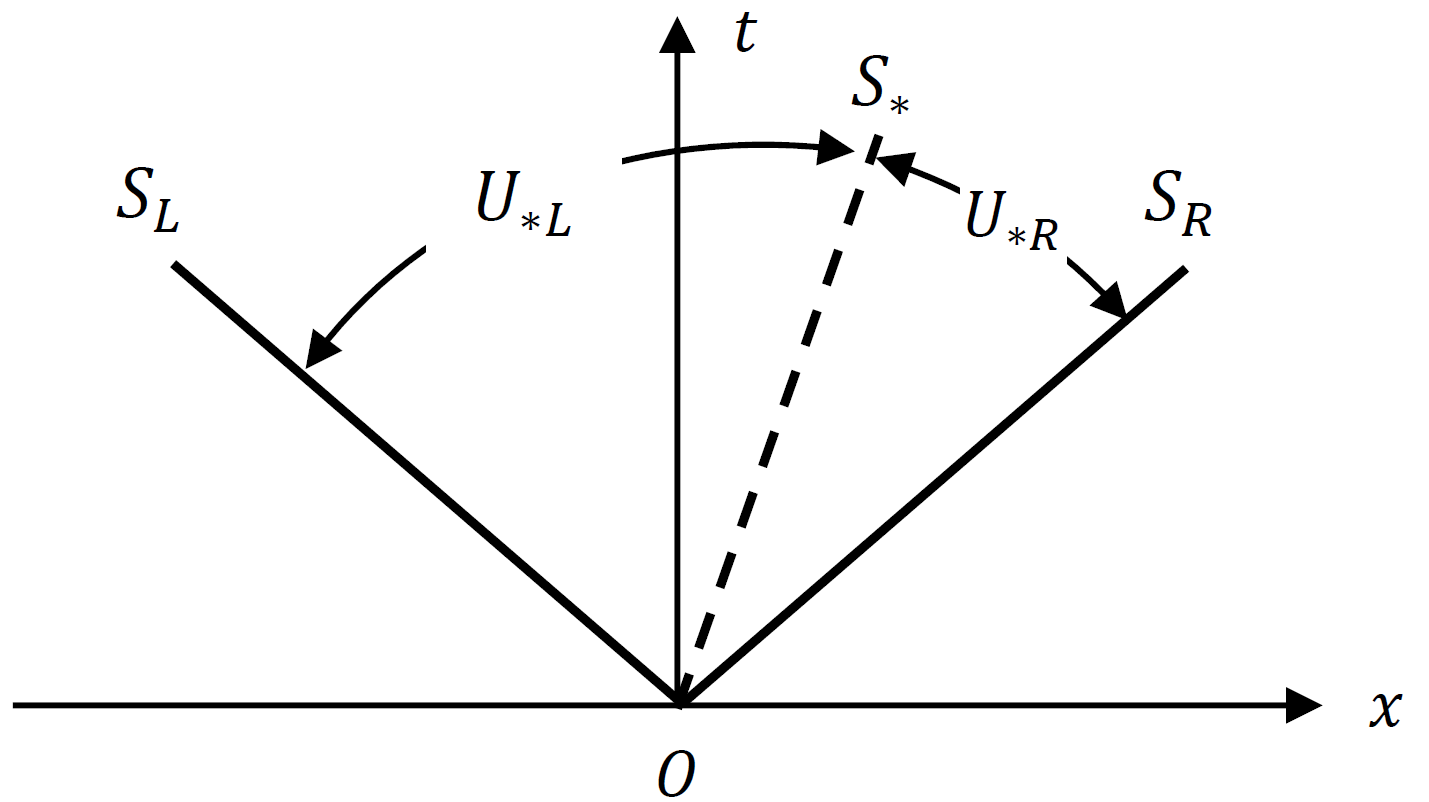
\includegraphics[width=0.75\textwidth]{numerical-scheme-figures/riemann-problem.png}
\caption{Diagrammatic representation of the approximate Riemann solution}
\label{RiemannProblem}
\end{figure*}

The full method is widely available, and is implemented exactly as described in \citet{Toro1994}, thus omitted here.

\subsection{Boundary conditions}

The extremities of the computational domain lack sufficient data to compute the numerical scheme, lacking neighbours on one or more faces. A variety of methods are available for the treatment of boundary conditions, it is far preferable numerically if the area of interest is sufficiently distant from the boundary, thereby reducing the influence of the method employed. The simplest approach is to prevent computation at the extremities and ensure these cells are dry; this is analogous to a waterfall in the real world, where flow is prohibited from returning. The Riemann solution across the interface is likely however to draw an excessive amount of water from upstream, which risks skewing nearby results.

For simulations where water must be contained within the domain, options are to reverse the flow direction and directly reflect flows, or create a wall using a high bed elevation which should also reflect flows albeit with some losses. The latter may prove more diffusive, but such an effect would also be expected in reality.

Boundary conditions describing river flows (i.e. a timeseries depth and discharge or velocity values) can either be introduced through the source term vector $\mathbf{s}$, or through careful manipulation of the cell states outside the numerical scheme. 

\subsection{Stability criterion}

The maximum permissible timestep for stability in the scheme is governed by the work of Courant-Friedrichs-Lewy \citep{Courant1967}, or the so-called CFL condition
\begin{equation}
	\label{CFL}
	\Delta t = C \cdot min \left[\frac{\Delta x}{\lvert u + \sqrt{gh} \rvert} , \frac{\Delta y}{\lvert v + \sqrt{gh} \rvert}\right] ,
\end{equation}
where \(C\) is the Courant number, with constraint \(0 < C \le 1\). The CFL condition is applied to all of effective computational cells, and the largest permissible time step is thereby used to advance the numerical scheme to the next time increment. It is worth noting the limitations of this approach, insofar as $\sqrt{gh}$ describes the phase velocity of shallow water waves, but the shallow water model presented herein will be applied across a range of scenarios. Shocks and discontinuities not fully addressed by Equation \ref{CFL} also become more likely at high grid resolutions, hence values of $C$ are typically kept below $0.7$ for the work herein, consistent with the findings of \citep{Erduran2002}. A halving in the grid size will result in a four-times increase in the number of cells, whilst also halving the CFL-constrained timestep, thus typically increasing simulation workload eight-fold.

\subsection{Source terms for energy loss and topographic slope}
\label{sec:source-terms}

The bed slope source terms are directly approximated by a central differencing approach. For example, in the $x$-direction,

\begin{equation}
	\label{SWE_1stO_BedSlope}
	-g \eta \frac{ \delta z_b }{ \delta x } = -g \tilde{\eta} \left ( \frac{ z_{bE} - z_{bW} }{ \Delta x } \right )
	,
\end{equation}

where $ \tilde{\eta} = ( \eta_{E}^{L} + \eta_{E}^{R} )^2 $. 

For the friction source terms, a splitting-limited-implicit scheme adopted by \citet{Liang2010a} is implemented to ensure better numerical stability. This gives a robust finite-volume Godunov-type solver for simulating shallow flows over complex domain topography with wetting and drying. The point-implicit scheme is given through Taylor expansion of an ordinary differential equation accounting for friction effects. This approach allows for a solution which is independent of the Godunov-type scheme. Neglecting higher-order terms in the expansion, unit-width discharges after accounting for friction become
\begin{equation}
	\label{Friction}
	\begin{alignedat}{3}
		&q_{x}^{t+\Delta t} && = q_{x}^{t} + \Delta tF_x && ,\\
		&q_{y}^{t+\Delta t} && = q_{y}^{t} + \Delta tF_y && ,\\
	\end{alignedat}
\end{equation}
where for axis \(x\) and perpendicular axis \(y\),
\begin{equation}
	\label{FrictionPrereq}
	\begin{alignedat}{2}
		&F_x      && = \frac{S_{fx}}{D_{dx}} ,\\
		&S_{fx}   && = -q_x\frac{C_f}{h^2}\sqrt{q_{x}^{2} + q_{y}^{2}} ,\\
		&D_{dx}   && = 1 + \Delta t \times \frac{C_f}{h^2} \times \frac{2q_x + q_y}{\sqrt{q_{x}^{2} + q_{y}^{2}}} ,\\
		&C_f      && = \frac{gn^2}{h^{\frac{1}{3}}} .
	\end{alignedat}
\end{equation}

\section{Extension to second-order solution}

A MUSCL-Hancock approach \citep{VanLeer1984} is adopted to achieve second-order accuracy in both space and time. Specifically, cell face-extrapolated values are obtained using a MUSCL linear reconstruction method implemented with a MINMOD slope limiter \citep{Roe1986} for flow variables \(\begin{matrix}[\eta & uh & vh]\end{matrix}^T\) to prevent spurious oscillations that might otherwise be introduced \citep{Toro2001}. This ensures the scheme is total variation diminishing (TVD). The MINMOD limiter is selected herein because its properties provide better numerical stability for a wide range of conditions \citep{Suresh2000,Yee2006}, and while it is also diffusive by way of comparison to alternative methods, the advantages in terms of stability were considered superior.

These choices were guided by \citet{Erduran2002}, where the authors conclude second-order accuracy is sufficient for almost all cases, including large discontinuities, and acknowledge that in practical applications stability may be compromised with Courant numbers exceeding $0.7$.

A half-timestep evolution of the cell states is introduced for each iteration, using slope-limited values extrapolated towards each of the cell interfaces. Considering each of the primitive variables composing $\textbf{u}$ in Equation \ref{SWE_1stO} piece-wise as $u$, along an axis, the slope ratio for a cell is computed as 
\begin{equation}
	\label{SWE_SlopeRatio}
	r_i = \frac{u_i - u_{i-1}}{u_{i+1} - u_i}
	.
\end{equation}
Each slope ratio is limited using the MINMOD function given by \citet{Toro2001}, which can be simplified for this application to give,
\begin{equation}
	\label{SlopeLimiter_MINMOD}
	\phi_{mm}(r) = max(0, min( 1, r_i ))
	.
\end{equation}
Piece-wise application of the slope functions, $\phi_{mm}(r)$, to the vector \(\begin{matrix}[\eta & h & uh & vh]\end{matrix}^T\) provides a slope vector $\mathbf{\bar{\Delta}}$, which is applied along each axis, giving two face-extrapolated vectors, $\mathbf{u}_i^L$ and $\mathbf{u}_i^R$ for each,
\begin{equation}
	\label{MUSCL_FaceExtrapolation}
	\mathbf{u}_i^L = \textbf{u}_i - \frac{1}{2}\mathbf{\bar{\Delta}}\hspace{4ex}, \\
	\mathbf{u}_i^R = \textbf{u}_i + \frac{1}{2}\mathbf{\bar{\Delta}}\hspace{4ex}
	.
\end{equation}

Application of the slope limiter along each axis provides a face-extrapolated vector for each Cartesian direction, \(\begin{matrix}u^N & u^E & u^S & u^W\end{matrix}\). These are used to advance the cell states by a half-timestep,
\begin{equation}
	\label{SWE_MUSCL_HalfTimestep}
	\begin{alignedat}{2}
	\mathbf{u}_{i,j}^{t+\Delta\frac{1}{2}} 
	=
	\mathbf{u}_{i,j}^{t}
	& - \frac{1}{2} \frac{\Delta t}{\Delta x} (\mathbf{f}(\mathbf{u}^E) - \mathbf{f}(\mathbf{u}^W)) \\
	& - \frac{1}{2} \frac{\Delta t}{\Delta y} (\mathbf{g}(\mathbf{u}^N) - \mathbf{g}(\mathbf{u}^S)) \\
	& + \frac{1}{2} \Delta t \mathbf{s} 
	\hspace{4ex},
	\end{alignedat}
\end{equation}
using modified functions to evaluate the flux, where the bed elevation is derived from the face-extrapolated vectors, as for $\mathbf{f}$ and $\mathbf{g}$ in Equation \ref{SWETerms_1stO}.

Friction terms can be omitted from the source terms at this point, and later applied using the point-implicit scheme in Section \ref{sec:source-terms}. The half-timestep advanced cell states are extrapolated using the same piece-wise application of slopes in Equation \ref{MUSCL_FaceExtrapolation} and carried forward for use evaluating the full-timestep with Riemann solutions.

The methods employed herein provide a second-order accurate solution under normal circumstances, but will fall back to a first-order solution at the wet-dry interface. The limiter function is constrained so as to ensure the solution remains within the TVD region. Research remains ongoing with regard to the treatment of wet-dry interfaces, avoidance of spurious velocity measurements, and maintaining numerical stability with high-order methods, such as in the work of \citet{Hou2013}.

\section{Solution using heterogeneous architectures}

The equations and methods described in this chapter thus far, given their iterative, time-marching and piece-wise nature, require the assistance of computers to be applied. The approximately eight-fold increase in computational expense for each halving of the grid resolution is problematic for application at high resolutions, in dense urban environments, and so prudence and considered software design is required to make these simulations feasible. As previously discussed, many computers offer either hybrid processor architectures, or more than one form of processor with different intended applications, most notably general computational and graphic rendering. The remainder of this chapter focuses on the software design approach required to map the numerical scheme to these processors, in an efficient manner.

\begin{figure*}[bp]
	\centering
	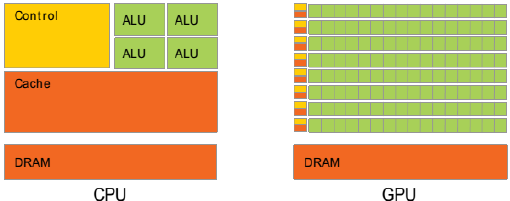
\includegraphics[width=0.7\textwidth]{numerical-scheme-figures/cpu-gpu-architecture.png}
	\caption{A simplified comparison of the differences between CPU and GPU architectures.}
	\label{CPUGPUArchitecture}
\end{figure*}

The GPU is so-named because its design and purpose is to accelerate graphics calculations, primarily 3D rendering such as in computer games. The calculations are performed within `shaders', small program designed to perform a specialised set of matrix calculations with uniform values (e.g. the position of the sun to calculate shadows) and vectors. A vertex shader is executed over all the vertices that form the 3D model, to compute a 2D on-screen position from the 3D world, and a fragment shader subsequently over each of the pixels, to compute lighting effects and sample textures. A smooth experience requires a throughput of up to 90 frames per second, hence these processors are highly specialised; shader programs typically do not change during execution, and may be executed simultaneously on enormous volumes of data, such as for the $\gtrapprox 1.3M$ pixels on a typical computer screen.

A simplified comparison of the two processor architectures is shown in Figure \ref{CPUGPUArchitecture}, where the far higher ratio of arithmetic logic units to control units is seen; this is because a single controller can instruct many logic units to perform the same calculation. This architecture is known as single-instruction multiple-data (SIMD). Their performance is typically measured in terms of floating point operations per second (FLOPS), although the difference between theoretical maximum and the rate achievable in practice (where data must be read and written) is usually substantial.

\begin{table*}[pb]
	\newcolumntype{R}[1]{>{\RaggedLeft\arraybackslash}p{#1}}
	\small
	\centering
	\caption{Comparison of some of the CPU and GPU devices employed in this thesis, with prices correct in 2013.}
	\label{CPUGPUCosts}
	\begin{tabular}{p{0.3\textwidth}R{0.2\textwidth}R{0.2\textwidth}R{0.2\textwidth}}
		\hline
										& \textbf{CPU} Intel i7 950 3GHz & \textbf{GPU} AMD FirePro V7800 ($\times$2) & \textbf{GPU} NVIDIA Tesla M2075 ($\times$4) \\
		\hline
		Cost							& £260						& £1,200						& £10,000			\\
		64-bit FLOPS $\times10^{9}$		& 49						& 806							& 2,064				\\
		Device memory (GB)				& N/A						& 4.0 (2.0 $\times$ 2)			& 24.0 (6.0 $\times$ 4) \\
		Cost per FLOP $\times10^{9}$		& £5.20						& £1.49							& £4.84				\\
		\hline
	\end{tabular}
\end{table*}

The advantages of leveraging GPU devices become more apparent when the costs are examined. Table \ref{CPUGPUCosts} outlines the cost per unit of computing power for some of the devices used herein, which for these cases are all capable of residing within a single computer (division of work across devices in more than one computer is discussed later). The GPU devices, whilst less versatile, provide more power per pound expended, although it is worth noting a GPU device cannot operate without a counterpart CPU, and most likely at least the same memory available to the CPU as GPU. The M2075 GPU represents a professional-grade device targeted at general-purpose computation rather than graphics, hence the greater cost.

\subsection{Control flow and software structure}

The Open Computing Language (OpenCL) is a consortium-led project involving multiple hardware vendors that allows developers to produce low-level code compatible with a variety of modern CPUs, GPUs and APUs (a hybrid-style processor allowing some of both benefits on a single chip) available from NVIDIA, AMD and Intel \citep{KhronosOpenCLWorkingGroup2012,NVIDIACorporation2010,AdvancedMicroDevicesInc2011}. The software developed herein uses OpenCL to provide the greatest compatibility between different device and hardware configurations, whilst the performance levels achievable are comparable to popular alternatives such as CUDA \citep{Fang2011}. Non-parallelised parts of the software were developed in C++. Differences in architecture, quantity of, and structure of compute units (which may be a core for a CPU, or a streaming multiprocessor for a GPU, depending on the manufacturer and architecture), and memories available thereon make it difficult to design code which can be considered optimised across a large number of devices. A new model structure is presented in this work to cope with these difficulties, and variations in memory management are assessed to determine their effect.

Successful and efficient implementation for GPUs requires careful consideration of the six elements shown in Figure \ref{ModelComponents}, where a kernel refers to a discrete function within the program that can be executed in parallel across a range of data, and a reduction entails identifying a single value (e.g. minimum, maximum, or sum) from a large number of elements. To address hardware differences properly, the software developed allows end-user configuration of floating-point precision, workload balance in data reductions, and caching from global to local memory where applicable. Unlike existing software, a suitable and optimised configuration should therefore be achievable for any device conformant to the OpenCL specification.

A regular Cartesian grid of \(M \times N\) cells is used. This reduces the total data requirement and computational burden as no structure is necessary relating cells, and trigonometric functions are not required to update cells. Static cell data and initial conditions for transient variables are read from raster files using the Geospatial Data Abstraction Library (GDAL), thereby providing support for most common GIS file formats. Device-specific binaries are compiled before each simulation with the system's OpenCL drivers, allowing pre-processor macros to define many constants including the domain dimensions. 

Code responsible for applying the finite-volume scheme is generated at least in part dynamically, then compiled by the underlying operating system drivers using an appropriate instruction set and optimisations for the hardware available, a process which typically takes $<1$ second. This is accomplished through the Application Programming Interface (API) functionality made available through the OpenCL standard. Relevant constants such as the cell dimensions of the domain are hence embedded in the assembly instructions themselves, and functionality which is not required or disabled (e.g. friction, atmospheric boundary conditions) can be removed altogether. Dynamic type definitions also allow the same codebase to be used with single- (32-bit) or double-precision (64-bit) floating-point arithmetic, which refers to the memory allocated to storing the significand and exponent to represent decimal numbers, in the manner employed by almost all modern computers, per IEEE 754 \citep{InternationalOrganizationforStandardization2011}.

A small overhead is associated with executing kernels and receiving notification of completion with blocking commands or callbacks. This is alleviated by adding multiple iterations of the numerical scheme to the execution queue and only displaying progress feedback periodically. Consequently, kernels are occasionally queued unnecessarily, as the simulation cannot progress further until output files are written; in such cases the timestep reduces to zero and kernels will exit early. The main loops operating on the compute device and host computer to coordinate this are shown in Figure \ref{HiPIMS_Structure_NoVis}, where there will be numerous iterations of the OpenCL loop before returning to the host computer loop.

\begin{figure*}[tpb]
	\centering
	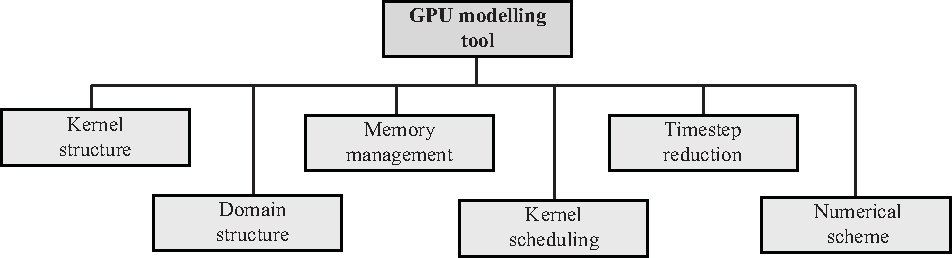
\includegraphics[width=0.95\textwidth]{heterogeneous-dev-figures/Figure_1_Greyscale.pdf}
	\caption{Main considerations for designing the shallow-flow modelling tool.}
	\label{ModelComponents}
\end{figure*}
\begin{figure*}[pb]
	\centering
	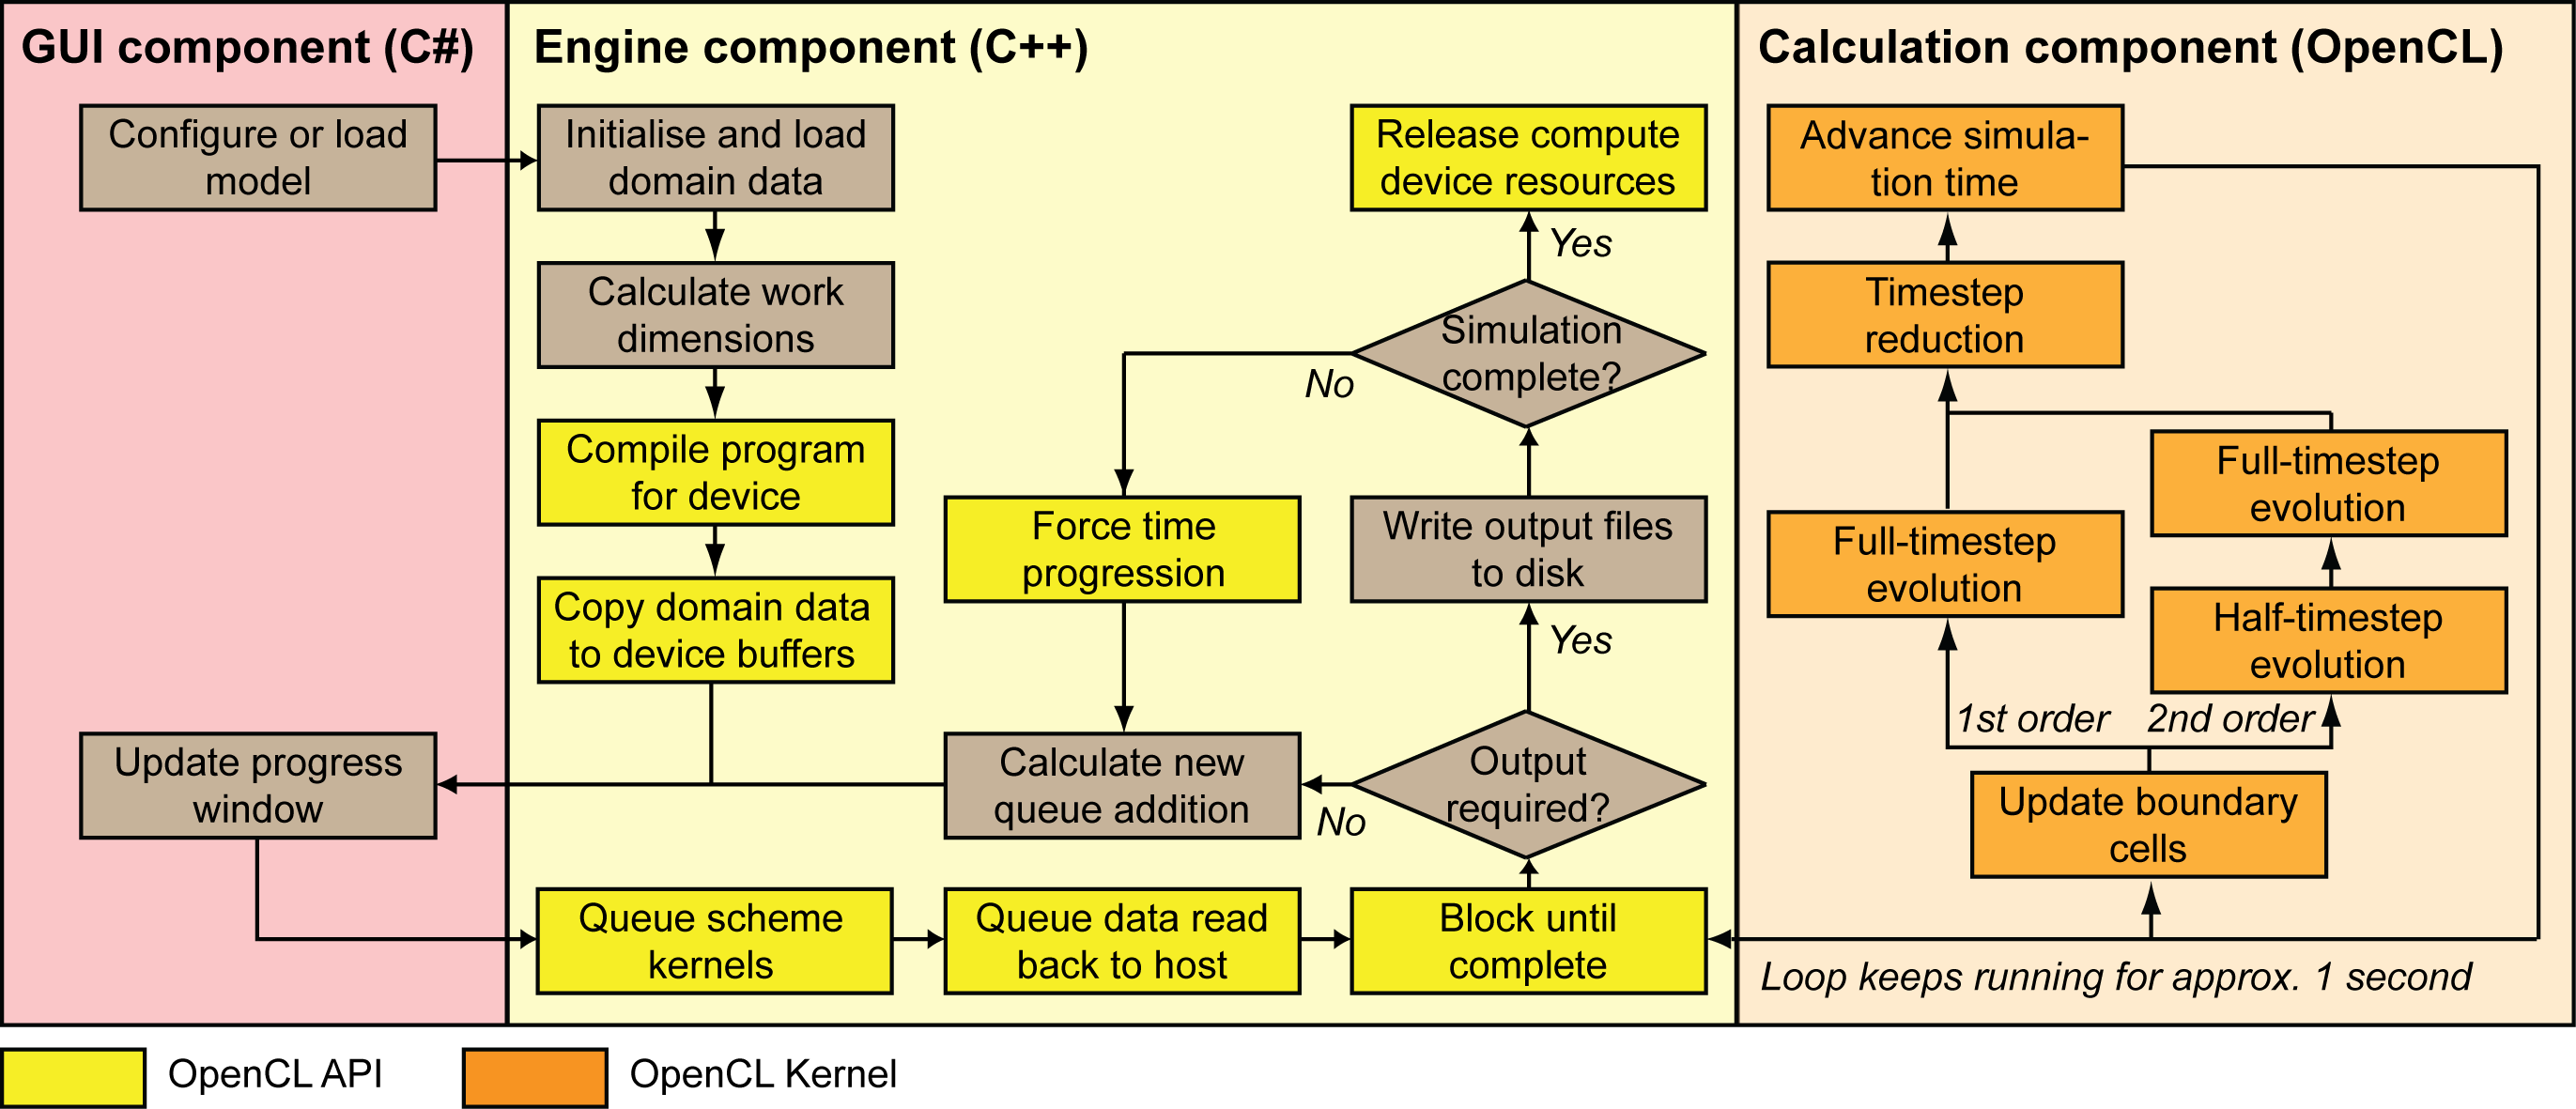
\includegraphics[width=1.0\textwidth]{heterogeneous-dev-figures/HiPIMS_Structure_NoVis.png}
	\caption{Flowchart of the software processes indicating which components are OpenCL kernels or API calls.}
	\label{HiPIMS_Structure_NoVis}
\end{figure*}

Moving data from the main system memory (RAM) to a GPU device is an expensive operation \citep[see recommendations in][]{AdvancedMicroDevicesInc2011,NVIDIACorporation2010a}. Cell data is only moved periodically for output files, and the numerical scheme is otherwise permitted to run in a loop for approximately one second before a small amount of data is transferred to update the user on the progress of the simulation. This process is represented in Figure \ref{HiPIMS_Structure_NoVis}. No vendor-specific optimisations were made, as the author's intention was to create a system appropriate for use with any of the mainstream vendors' hardware, most notably NVIDIA, AMD and Intel, but any conformant implementation of the OpenCL 1.2 standard should be capable of running the code. The compiler is instructed to adhere to all of the appropriate IEEE standards for floating-point arithmetic (i.e. accurate square root operations, treatment of denormals, etc.).

A regular Cartesian grid is used to represent the domain, whereby transient state variables are stored in a four-element vector and constant values (bed elevation and friction coefficients) require two further elements. This means 48 bytes or less are required per cell. Considering further constraints imposed on the size of a single memory allocation, the software is presently limited to $\approx$130 million cells for current hardware offering up to 16GB of memory.

A variety of raster formats are supported for importing and exporting domain data, initial conditions, and periodic output. 

\subsection{Identification of CFL-constrained timestep}

A two-stage reduction process is used to identify the largest permissible timestep within the domain: cells are sampled with a regular stride through the array of cells, followed by recursive binary comparisons used to provide a single value which is carried forward to a much smaller array, as shown in Figure \ref{HiPIMS_Reduction}. This is examined in the second stage when incrementing the overall simulation time. The reduction process ensures processors perform sufficient work to mask the considerable latency introduced by transferring data from a GPU's globally-accessible memory to compute unit-specific registers.

\begin{figure*}[tpb]
	\centering
	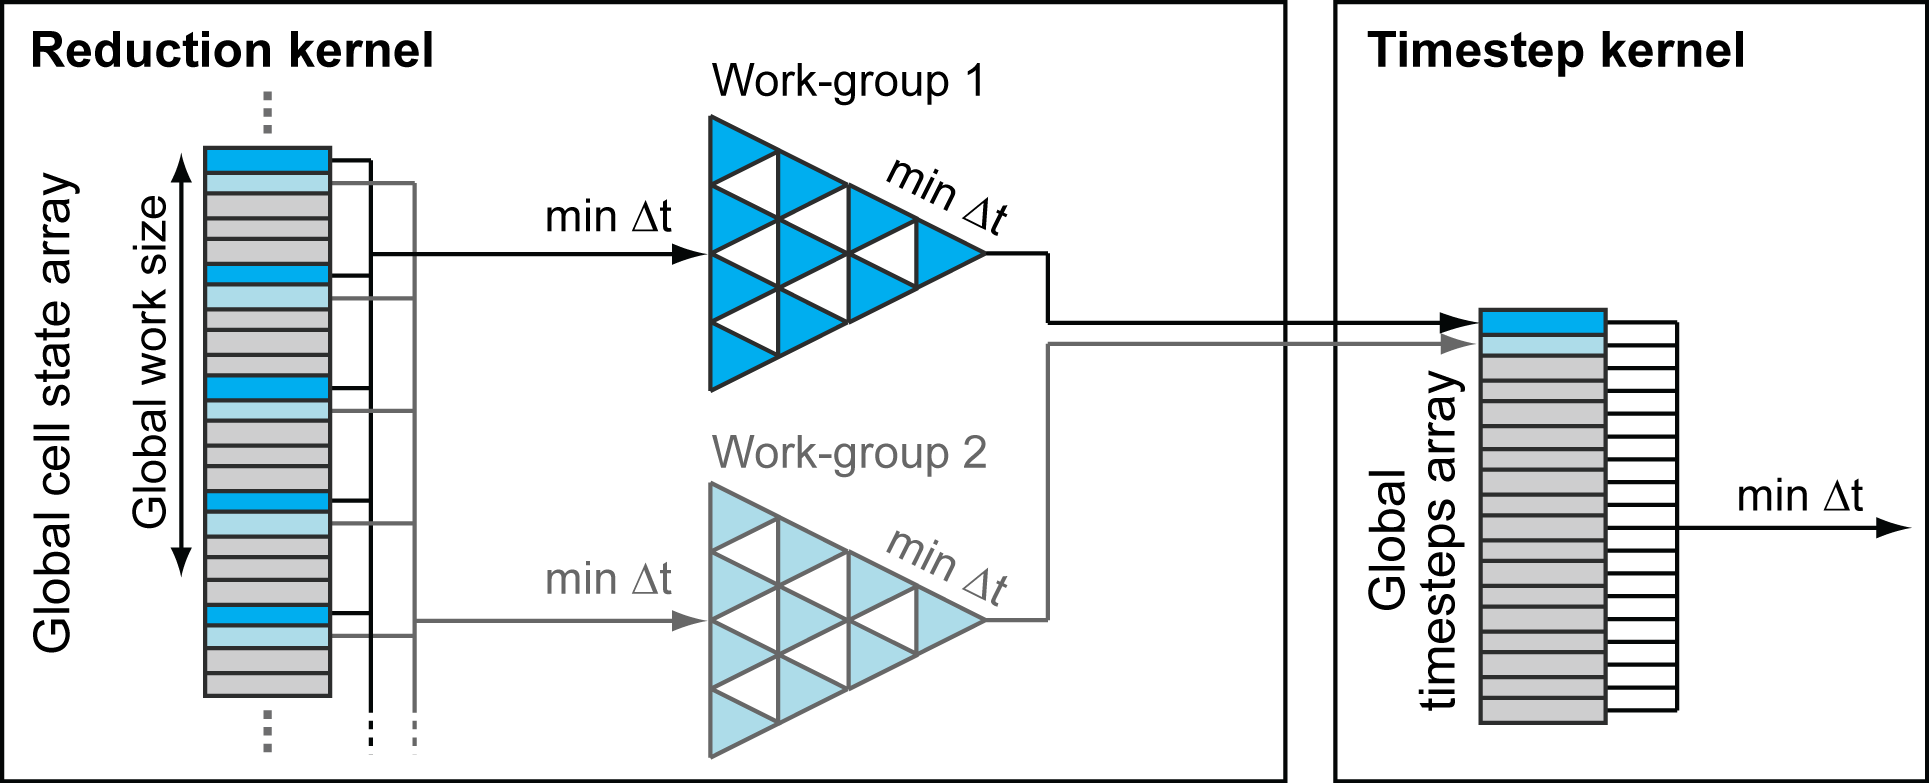
\includegraphics[width=0.8\textwidth]{heterogeneous-dev-figures/HiPIMS_Reduction_Colour.png}
	\caption{Representation of a two-stage reduction process with a global stride of six (stride in reality would be much larger) performing a series of binary comparisons to create a smaller array of potential values.}
	\label{HiPIMS_Reduction}
\end{figure*}

\subsection{Storage and memory access patterns in a heterogeneous environment}
\label{Subsection:StorageMemoryHeterogeneous}

The memory model adopted in OpenCL is composed of private (i.e. registers), local (or LDS), and global (including constant) memory; Figure \ref{OpenCLStructure} is a simplified representation of these memories. Global memory is the largest resource in which all data that persists throughout the simulation must reside. Scientific GPUs presently offer up to 16GB of global memory.

\begin{figure*}[tpb]
	\centering
	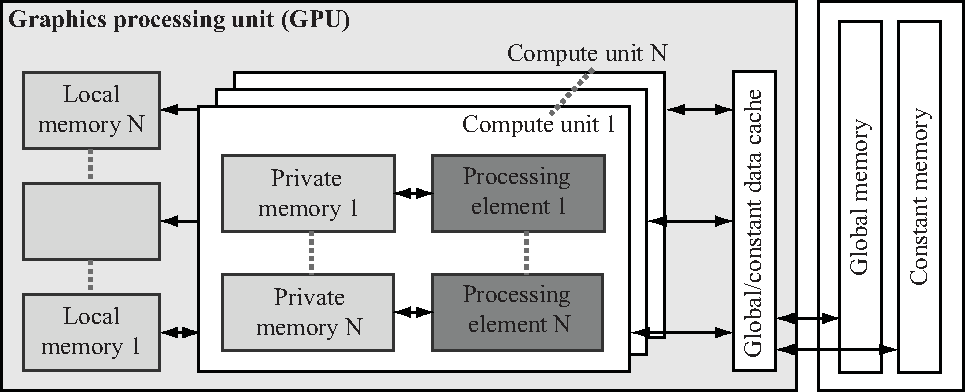
\includegraphics[width=0.8\textwidth]{heterogeneous-dev-figures/Figure_2_Greyscale.pdf}
	\caption{Memory model adopted in OpenCL, representing the structure of a GPU device and its global, local, private, and constant memory.}
	\label{OpenCLStructure}
\end{figure*}

The scheme used herein is directionally unsplit, thus both axes are considered simultaneously by kernels. A first-order solution is therefore dependent on data from four neighbouring cells, but a second-order solution is dependent on data from twelve cells, which as demonstrated in Figure \ref{RequisiteCellData} requires accessing global arrays using irregular strides. An alternative solution that reduces global accesses per cell is to commit cell data to local memory, synchronise the work-group, and subsequently access only that resource for neighbour data. 

\begin{figure*}[tpb]
	\centering
	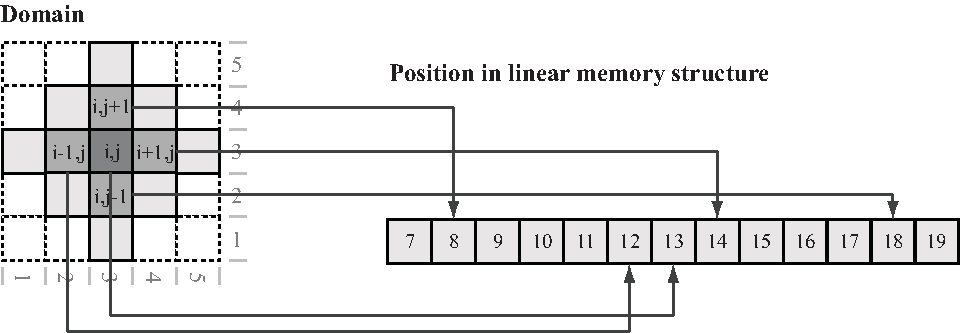
\includegraphics[width=1.0\textwidth]{heterogeneous-dev-figures/Figure_3_Greyscale.pdf}
	\caption{Requisite neighbour cell data to advance cell (i,j) demonstrating irregular strides when accessing global arrays, for a second-order solution.}
	\label{RequisiteCellData}
\end{figure*}

The minimum amount of local memory available for devices conformant to the OpenCL specification is 32kB, but maintaining activity on at least four work-groups requires each kernel to consume 8kB or less of local memory. Committing cell data for the whole work-group to local memory using a typical GPU work-group size of 256 hence allows for only 32 bytes of data per cell (i.e. four double-precision values).  This is insufficient to store four sets of cell face-extrapolated half-timestep advanced values. Moreover, cells towards the extremity of a work-group cannot be solved using the data in the local cache because neighbours are absent, so work-groups are required to overlap and the global work size is increased accordingly. Without caching, the whole work-group can be considered productive and no overlap is required. Caching for a prediction kernel requires a single layer overlap and increases the global work size by 30\% for a work-group size of 256, whereas caching for the whole computation in a single kernel is both arithmetically intensive and requires a double layer overlap, drastically increasing the global work size by 78\%. To address these constraints in this work, face-extrapolated data are held only in global or private memory depending on the configuration. Similarly, conserved variables may be configured as cached to local memory or read directly from global memory.

Finally, local memory on GPUs is divided into banks (typically 16 or 32); serialisation is required for accesses to addresses in the same bank (i.e. conflicts). These can be avoided by manipulating the dimensions of the cache array to introduce padding, but the increased memory consumption may reduce the number of schedulable units running simultaneously.

\subsection{Decomposition to stencil operations}

GPU architectures were designed and intended for graphical applications, especially rendering 3D objects in a 2D plane, as discussed earlier in this chapter. These operations are referred to as stencil operations, where the element under consideration is dependent only on constants (e.g. the position of the camera in 3D, or the timestep for fluids) and its neighbouring elements.

\begin{figure*}[tpb]
	\centering
	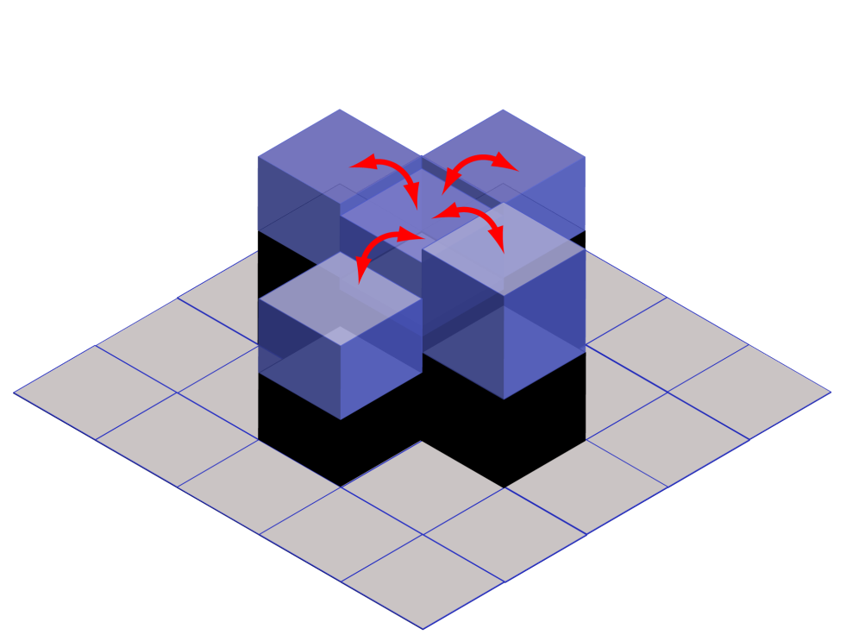
\includegraphics[width=0.95\textwidth]{heterogeneous-dev-figures/Stencil_Operation.png}
	\caption{Representation of the stencil operation with one cell dependent on its neighbours and fluxes between.}
	\label{StencilOperation}
\end{figure*}

Considering the first-order solution to the SWEs from earlier in the chapter, this can be expressed per Figure \ref{StencilOperation} as a series of stencil operations:
\begin{itemize}
	\item calculate fluxes between the cell of interest and each of its four neighbours;
	\item calculate the effect of those fluxes on discharge and free-surface level for the cell of interest, and apply the change.
\end{itemize}

The first-order solution with the HLLC method is dependent on four neighbouring cells; the data requirements are significant, and will affect computational performance.

The above method can be extended for the second-order solution, in which each neighbouring cell is also dependent on its neighbours. The overall data requirements increase accordingly to twelve neighbouring cells, but if the whole process is considered as two steps, the half- and full-timestep, then each step remains dependent on only four neighbouring cells with an additional requirement to store data between the two steps.

A kernel in OpenCL is executed over the global work (i.e. whole domain), within which there are work-groups of work-items, as shown in Figure \ref{OpenCLExecStructure}. A different work-item therefore handles each cell in the domain with reference to data held for neighbouring cells. For a GPU, work-groups are decomposed to schedulable units of wavefronts (so-termed by AMD, not to be confused with actual waves) or warps (NVIDIA) for execution; specifics and vendor differences can be found in \citet{KhronosOpenCLWorkingGroup2012,NVIDIACorporation2010,AdvancedMicroDevicesInc2011}. Each processing unit should be constantly engaged in productive computation to achieve the best performance with GPU architectures, known as the level of occupancy. It requires that each processing unit is assigned multiple schedulable units, allowing high-latency operations (e.g. global memory accesses, which are equivalent to hundreds of clock cycles \citep{NVIDIACorporation2010}) to be masked by the device's scheduling. Occupancy generally benefits from a high ratio of arithmetic operations to global data accesses but scheduling further units delivers no further benefit once a high occupancy is already achieved \citep{AdvancedMicroDevicesInc2011}. Consequently there is no panacea for optimisation on every device when transposing the numerical scheme to kernels.

\begin{figure*}[tpb]
	\centering
	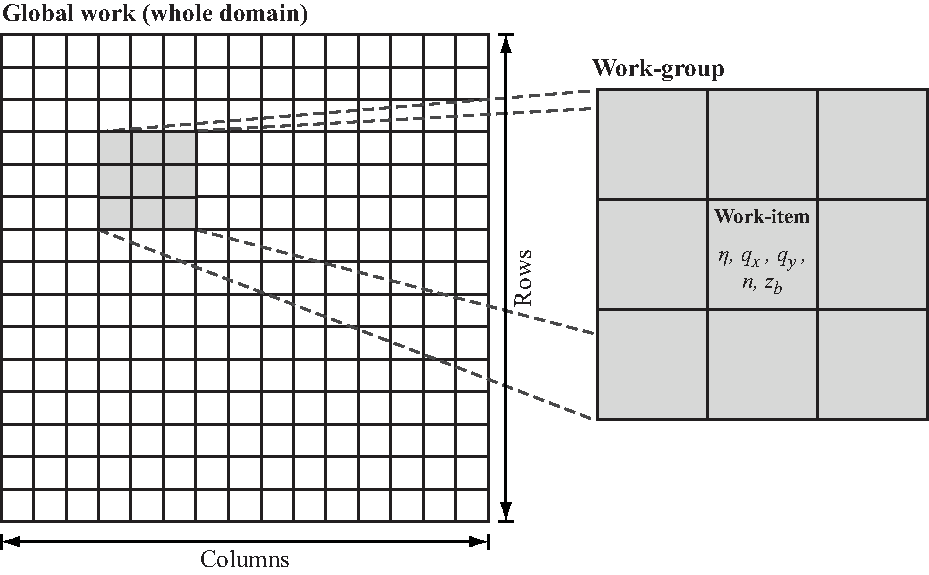
\includegraphics[width=1.0\textwidth]{heterogeneous-dev-figures/Figure_4_Greyscale.pdf}
	\caption{Structure of the OpenCL execution model as applied to the numerical scheme and domain structure herein.}
	\label{OpenCLExecStructure}
\end{figure*}
\begin{figure*}[tpb]
	\centering
	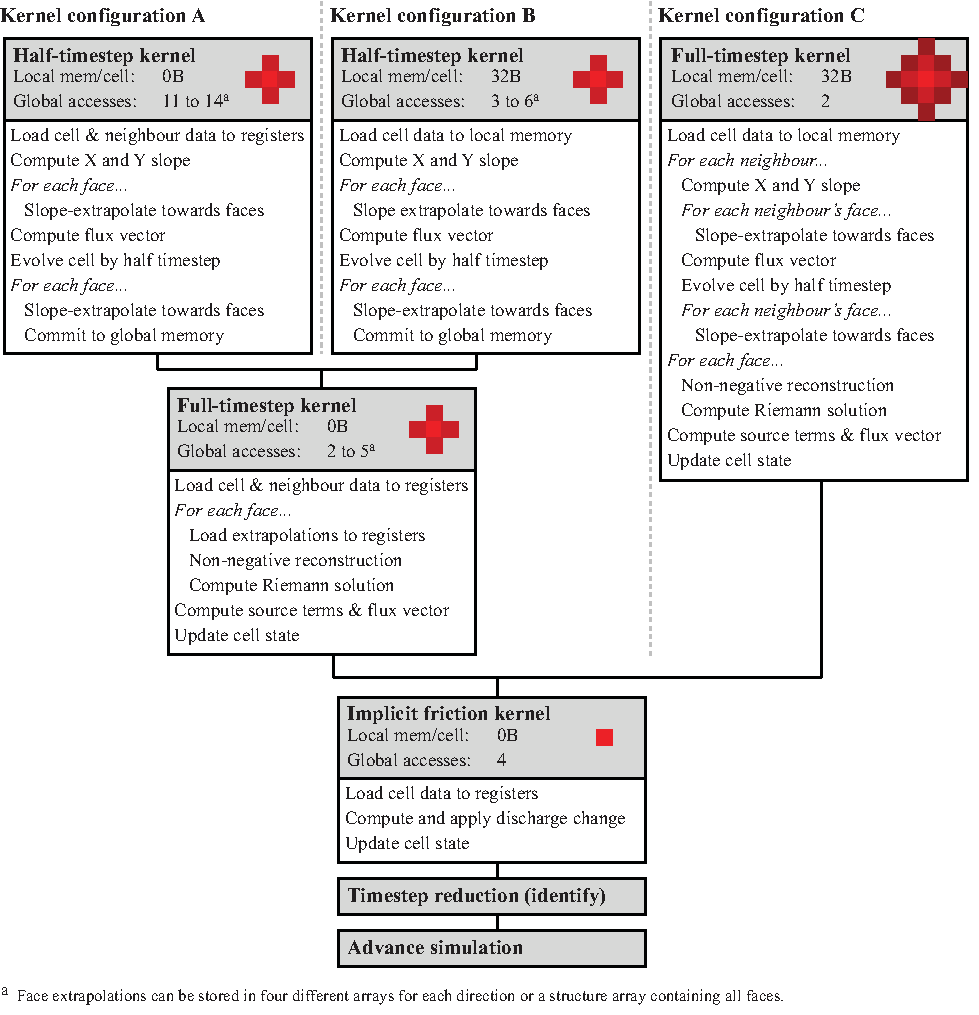
\includegraphics[width=1.0\textwidth]{heterogeneous-dev-figures/Figure_5_Colour.pdf}
	\caption{Implementation of the second-order MUSCL-Hancock scheme with three different kernel configurations intended to suit a majority of modern processing devices, and the data stencils for cell data required by each.}
	\label{Kernels}
\end{figure*}

To achieve high efficiency regardless of vendor differences, user-selectable kernel configurations are implemented to explore the effects of memory access patterns, illustrated in Figure \ref{Kernels} alongside the data stencils for each kernel. Configuration A is expected to perform well for devices with a high occupancy and sufficient resources to maintain enough warps/wavefronts to mask global memory latency, thus makes no use of local caching; configuration B introduces some caching to configuration A where possible in the half-timestep kernel, reducing the number of global accesses with irregular strides; and configuration C uses the maximum amount of caching and the least amount of global accesses, but the consequence is a greater computational burden because the half-timestep calculation must be repeated many times given that local memory is insufficiently sized to cache face extrapolated data. All high-end devices are expected to have enough resources (mainly registers) to perform best with configuration A. 

\section{User interface and platform availability}

\begin{figure*}[tpb]
	\centering
	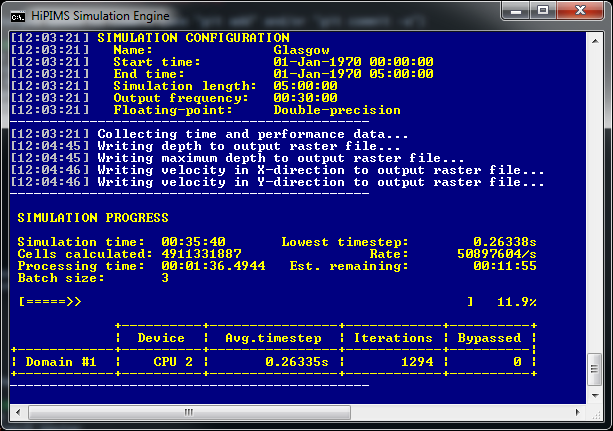
\includegraphics[width=0.9\textwidth]{software-figures/console-screenshot.png}
	\caption{Console-based version of the software, showing cell throughput on a CPU and the overall progress.}
	\label{Software_UI_Console}
\end{figure*}
\begin{figure*}[tpb]
	\centering
	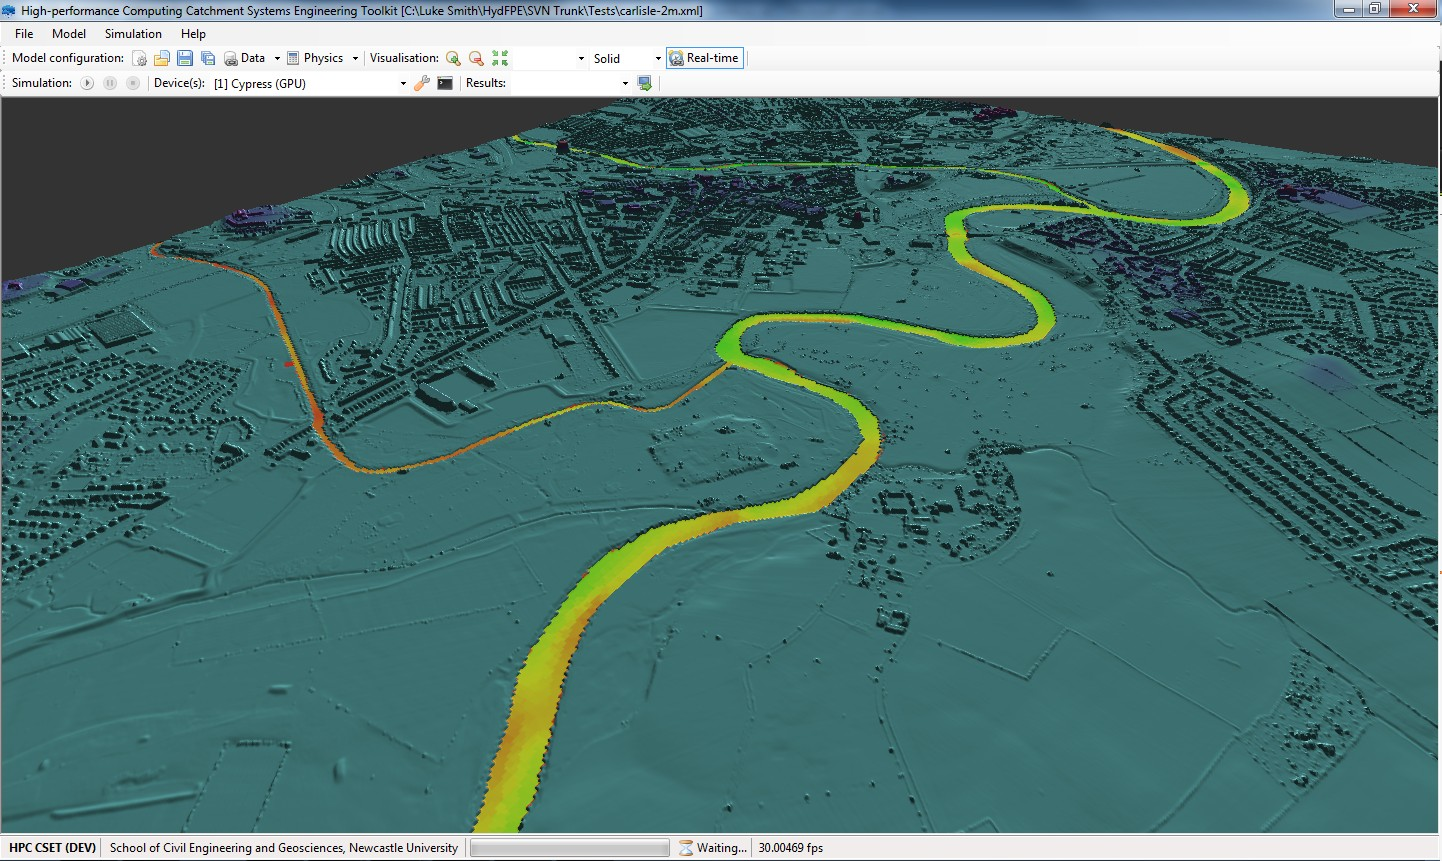
\includegraphics[width=1.0\textwidth]{software-figures/interface-screenshot.jpg}
	\caption{Windows-based version of the software, with real-time 3D visualisation of results, showing the initial state for a simulation of the Carlisle 2005 flood.}
	\label{Software_UI_3D}
\end{figure*}

Whilst non-contributory with respect to the fundamental research this thesis intends to provide, two user interfaces exist for the software. It is anticipated that the vast majority of applications for the software will be applied using high-performance computing servers, which are likely to only be accessible by console. A colour-enabled status console is provided, to report log messages, remaining time estimates, and overall simulation progress, as shown in Figure \ref{Software_UI_Console}. The software may be compiled for both Windows and Linux, for deployment to 32-bit and 64-bit architectures.

A more user-friendly interface already exists, capable of showing real-time simulation results in 3D, as in Figure \ref{Software_UI_3D}. A hue-based colour ramp is used to illustrate increasing depth. This interface uses a library-based version of the simulation engine, embedded within a C\# interface for consistency with other Windows applications, and OpenGL for 3D visualisation. Methods for improving the communication of simulation results are worthy of further research and discussion, but fall outside the scope of this thesis.

\section{Conclusions}

This chapter presented the numerical basis for a finite-volume solution to the shallow water equations, obtained using the HLLC method for approximately solving the Riemann problem, and thus creating a Godunov-type scheme. This is then extended to provide a second-order solution, by employing the MUSCL method. This computationally-intensive but versatile method is decomposed to stencil operations, such that each cell within the Cartesian domain is dependent only on a small number of neighbouring cells, and identification of the timestep from all cells in the domain is performed using a two-stage process which allows the processing to be shared across computing resources available. A number of different implementation patterns for the second-order solution allow caching to be leveraged, depending on the processing device employed.

The software described is capable of operating on CPU, GPU, and hybrid-style APU processing devices. The numerical and computational approach described is intended to make the software as versatile as possible, although there are nonetheless limitations to its applicability. The next chapter considers a wide range of flow scenarios and flood mechanisms, and evaluates the software's performance against each.
\chapter{Validation and performance assessment for single-domain simulations}
\label{chapter:NumericalValidation}

The aforementioned numerical schemes (first- and second-order) and the computational techniques employed to facilitate them require testing against a suite of recognised results, encompassing numerical and laboratory solutions, and those used in the industry as comparators. This chapter provides brief results for a range of test cases, chosen to represent some of the most challenging problems relevant to urban environments, and discussion with particular regard to accuracy. Where appropriate, the computational performance implications are also discussed.

The results were obtained using an AMD FirePro V7800 GPU with 2GB of memory, an Intel Xeon E5-2609 2.40GHz quad-core CPU with access to 24GB of memory, and an NVIDIA Tesla M2075 GPU with 6GB of memory. The value of \(g\) is taken to be 9.81ms\(^{-2}\). Comparisons are drawn between three different hardware devices from each of the mainstream manufacturers for the same numerical scheme and codebase. Timestep reduction is carried out using 200 work-groups of the maximum size each device will support.

The examples presented were selected because of their suitability for use in an automated test suite, whereby the simulation and expected results can easily be compared with code (e.g. well-balanced property, moving wet-dry fronts, dam-break against emerging bed), and to allow comparison with results published for implementations of comparable numerical schemes, and software widely used in industry (e.g. pluvial flooding in Glasgow, Malpasset dam collapse).

\section{Ensuring the well-balanced property}

In a situation where calm water is not expected to move, fluxes should cancel, regardless of the depth of water, and no change in free-surface level is expected. This is the well-balanced property.

A complex topography is used, in the form of a parabolic hill in the centre of the domain, representing an island within a sea. The external boundary of the domain is closed so no water may leave the domain. An initial free-surface level is set at $\eta = 0m$, with a sea depth of $s = 50m$ and the centre of the centrally-positioned island, at elevation $i = 100m$. The island itself is thus initially dry, and this situation is expected to persist, calculated on the basis,

\begin{equation}
\label{Test_WellBalanced_Conditions}
z_b = max \left( i - \left( b \times \frac{x^2 + y^2}{a^2} \right), \eta - s \right)
,
\end{equation}
and using the shape and scaling constants $a = 2000$, $b = 5000$.

The results after a 10 minute period are shown in Figure \ref{TestResult_WellBalanced}. This test focuses on the wetting and drying capability, for which fluxes will be calculated but should effectively cancel to provide no change in water level or velocity. The resultant depths remain unchanged, velocities are zero, and fluxes are balanced.

\begin{figure*}[tpb]
	\centering
	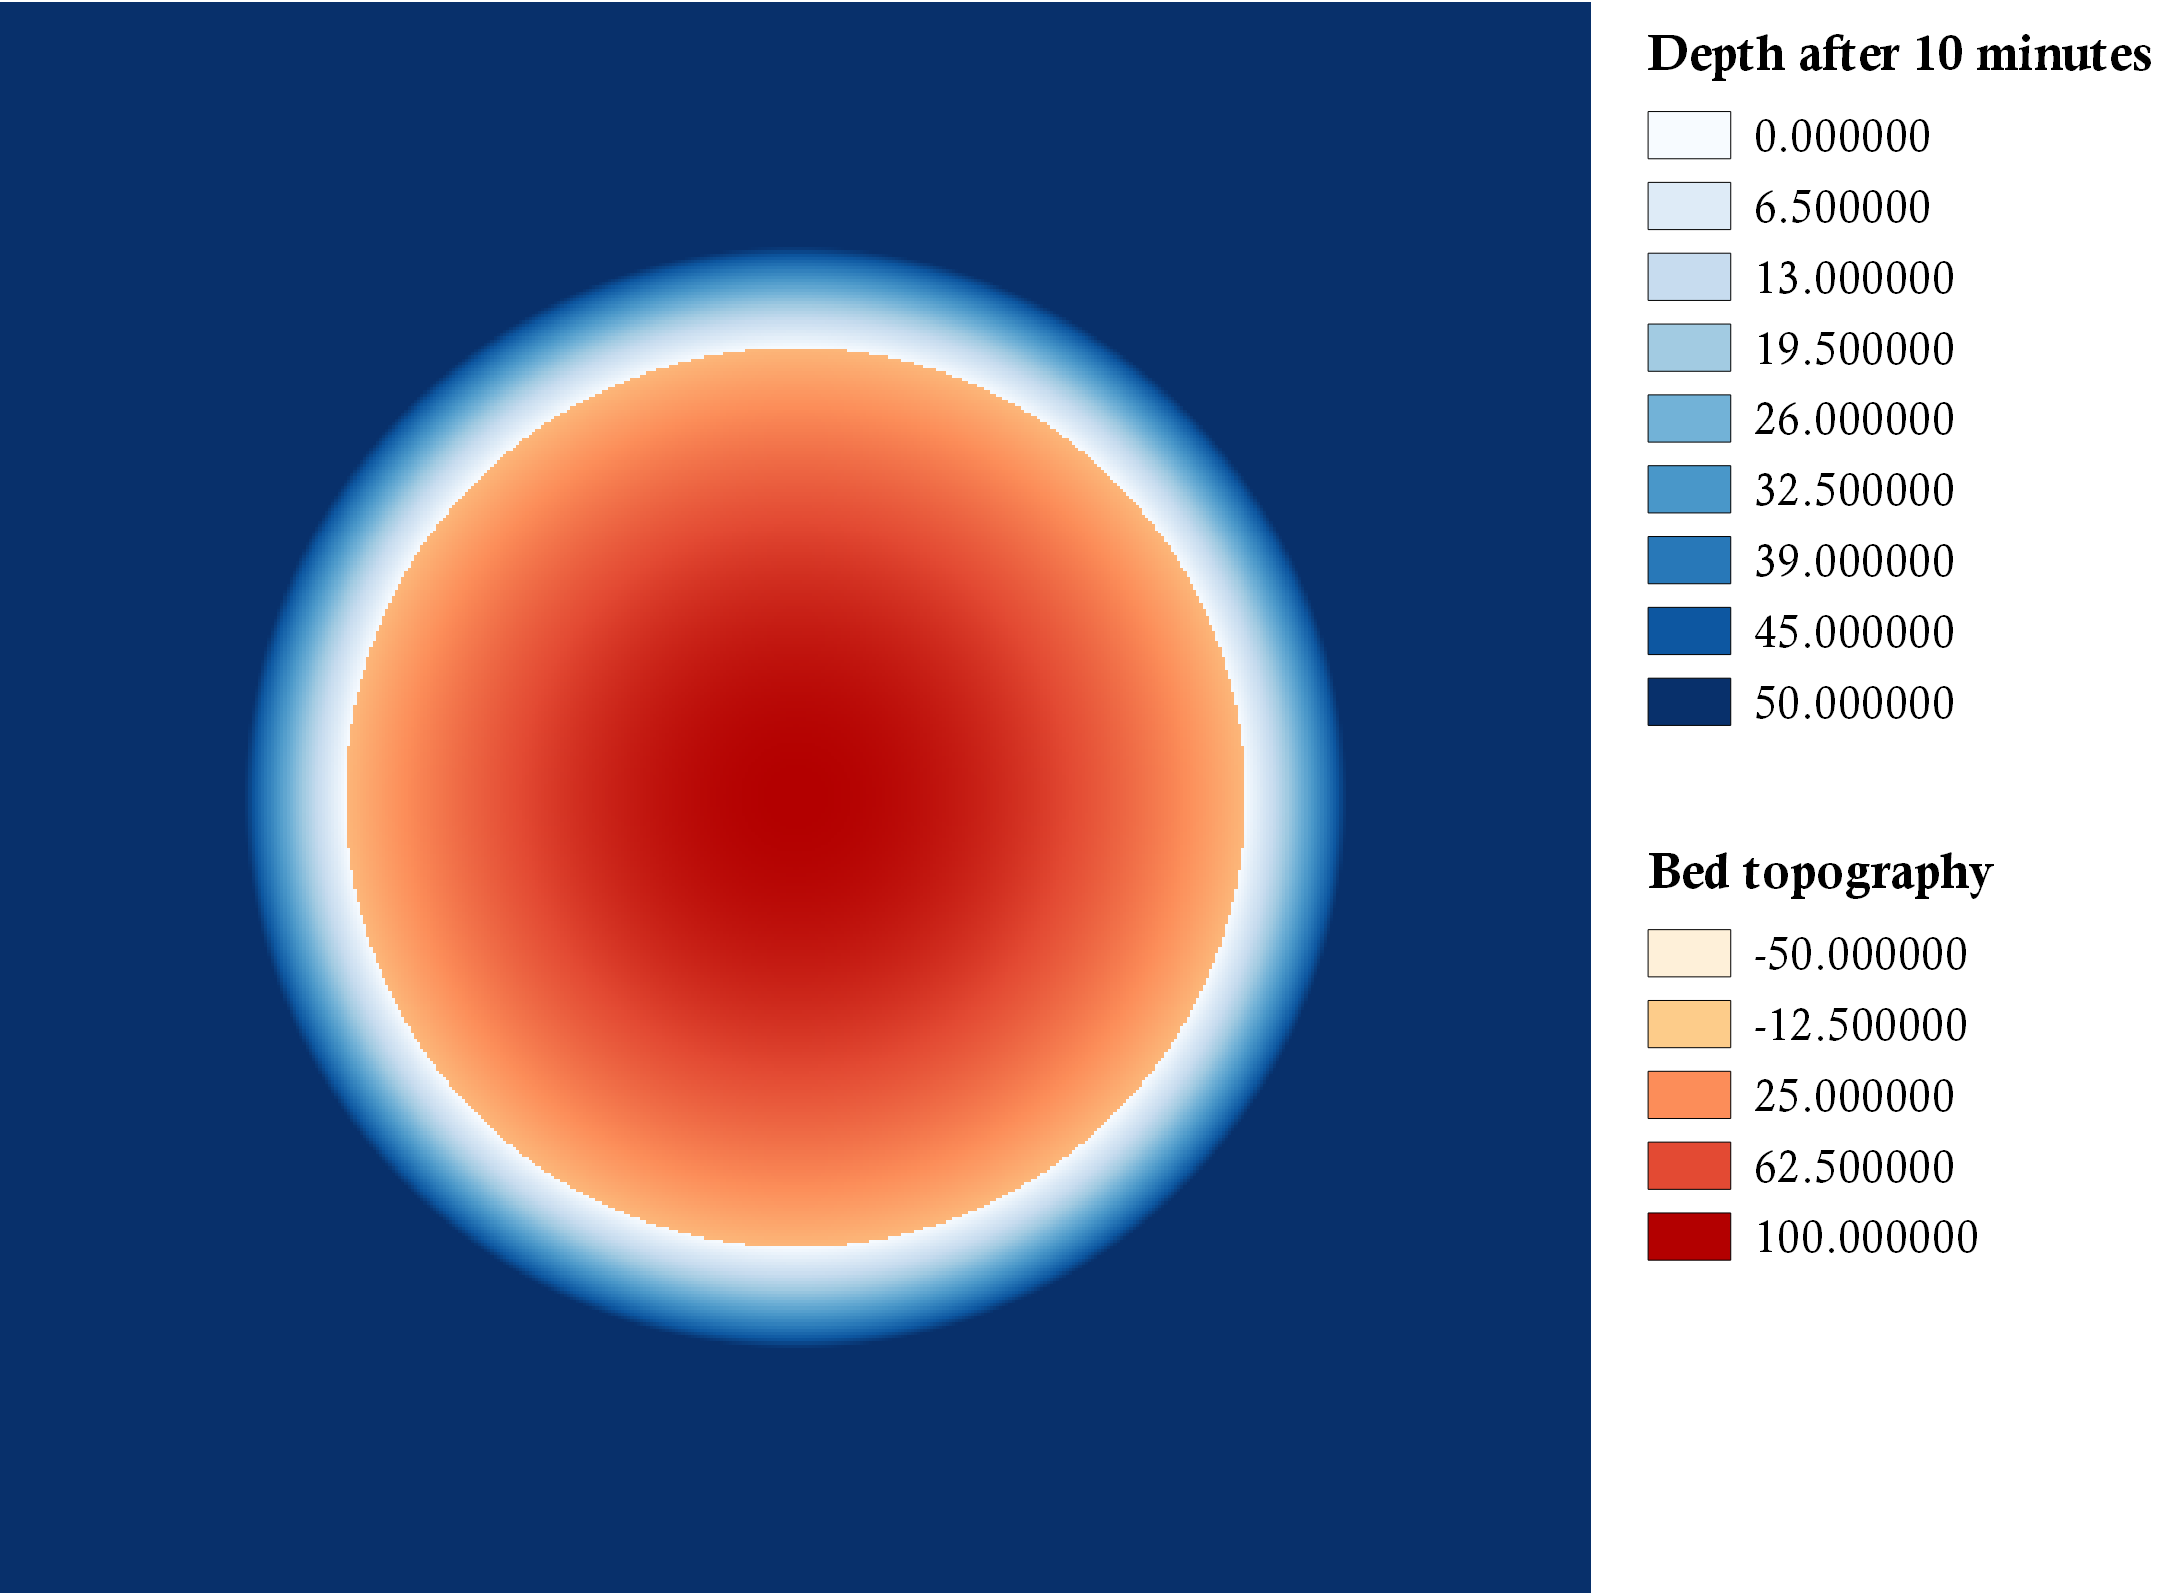
\includegraphics[width=0.9\textwidth]{numerical-test-figures/well-balanced-10mins.png}
	\caption{Depth within the domain after a 10 minute period, with the high points of the topography seen dry in the centre.}
	\label{TestResult_WellBalanced}
\end{figure*}

\section{Moving wet-dry fronts}

\begin{figure*}[tpb]
	\centering
	\begin{tabular}{cc}
		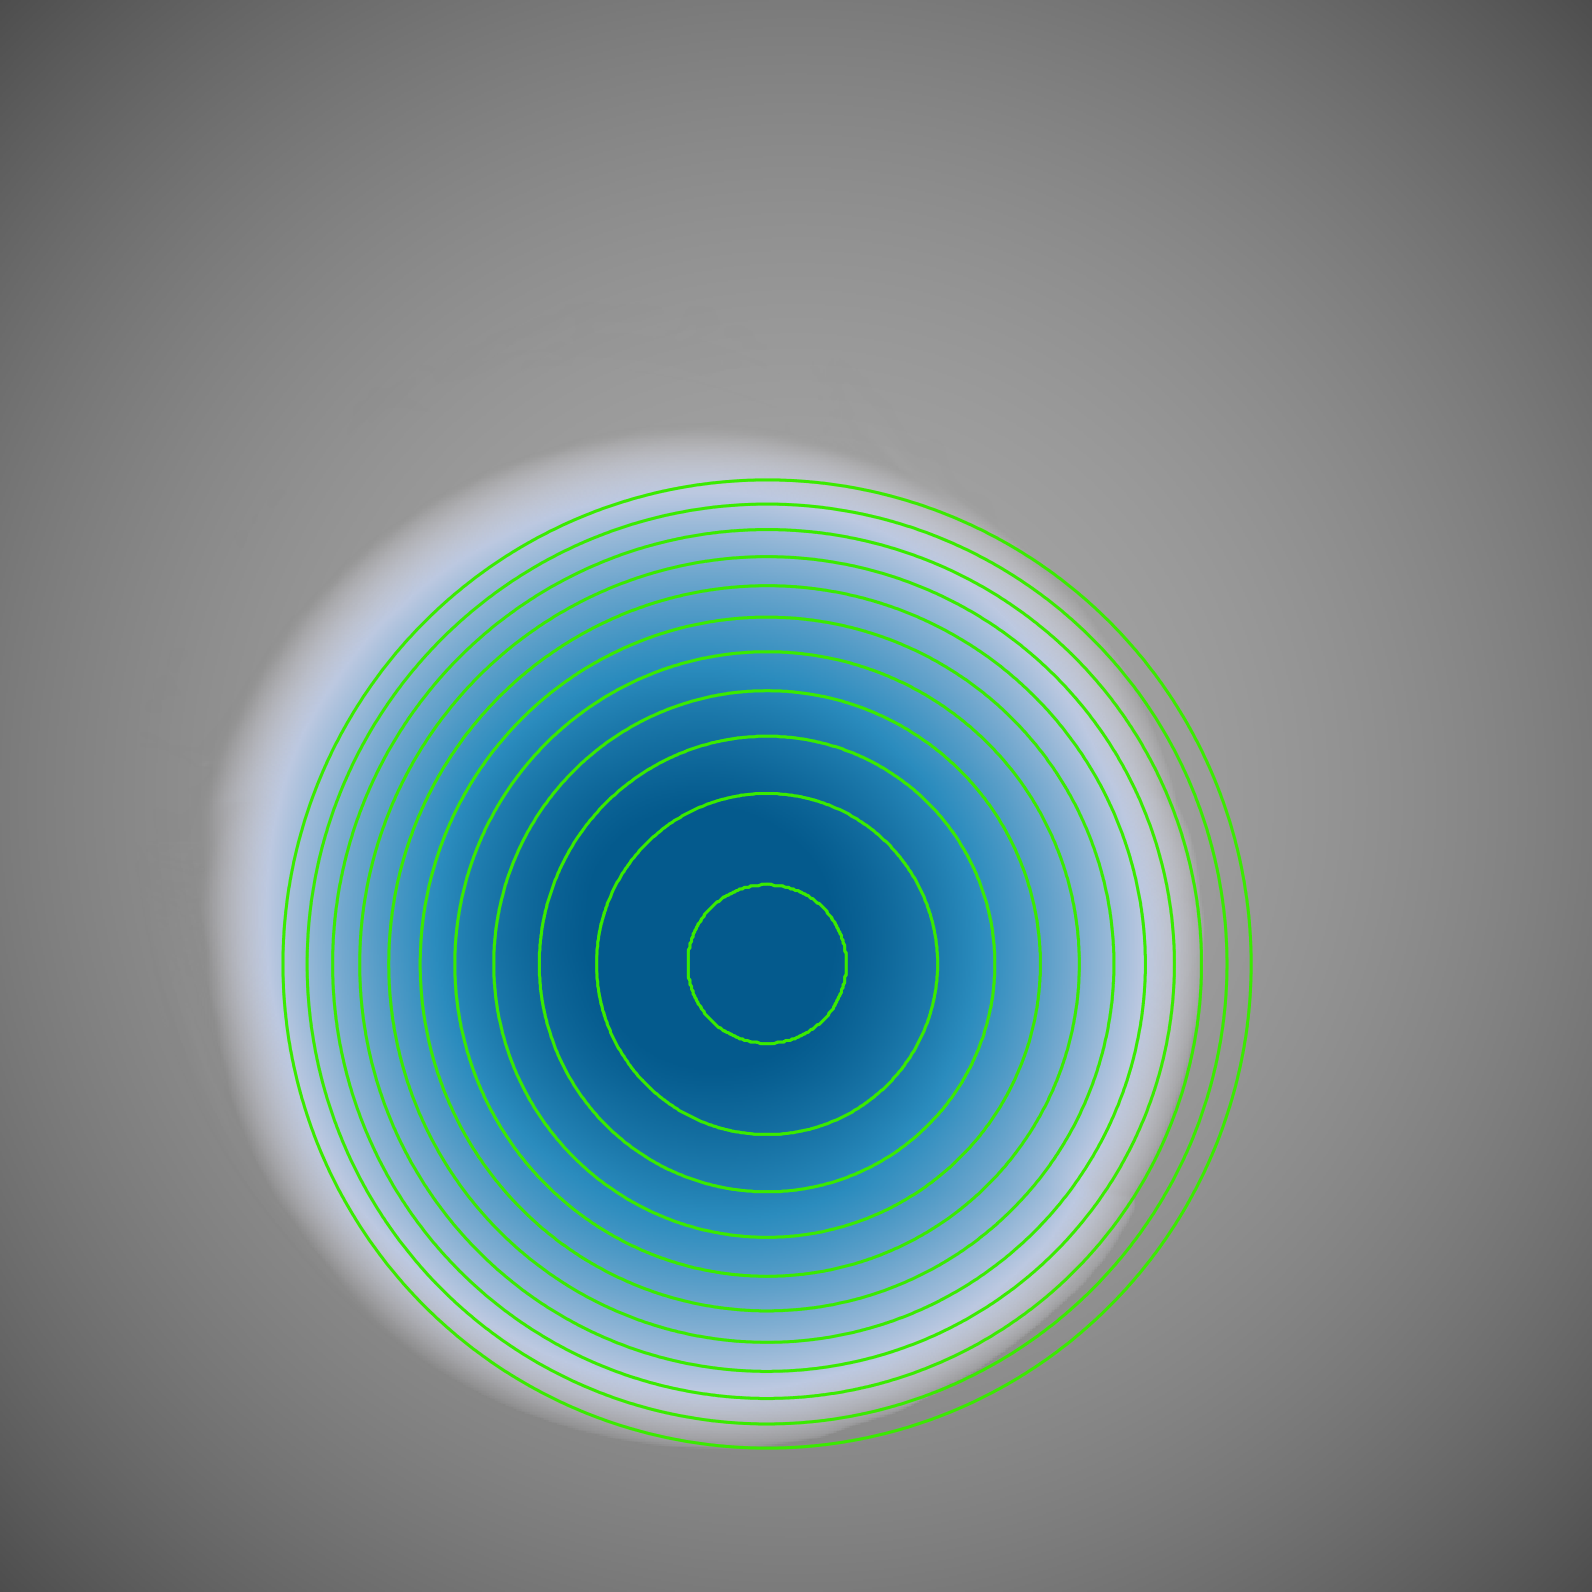
\includegraphics[width=0.4\textwidth]{numerical-test-figures/parabolic-bowl-1O-depth-300s.png} &
		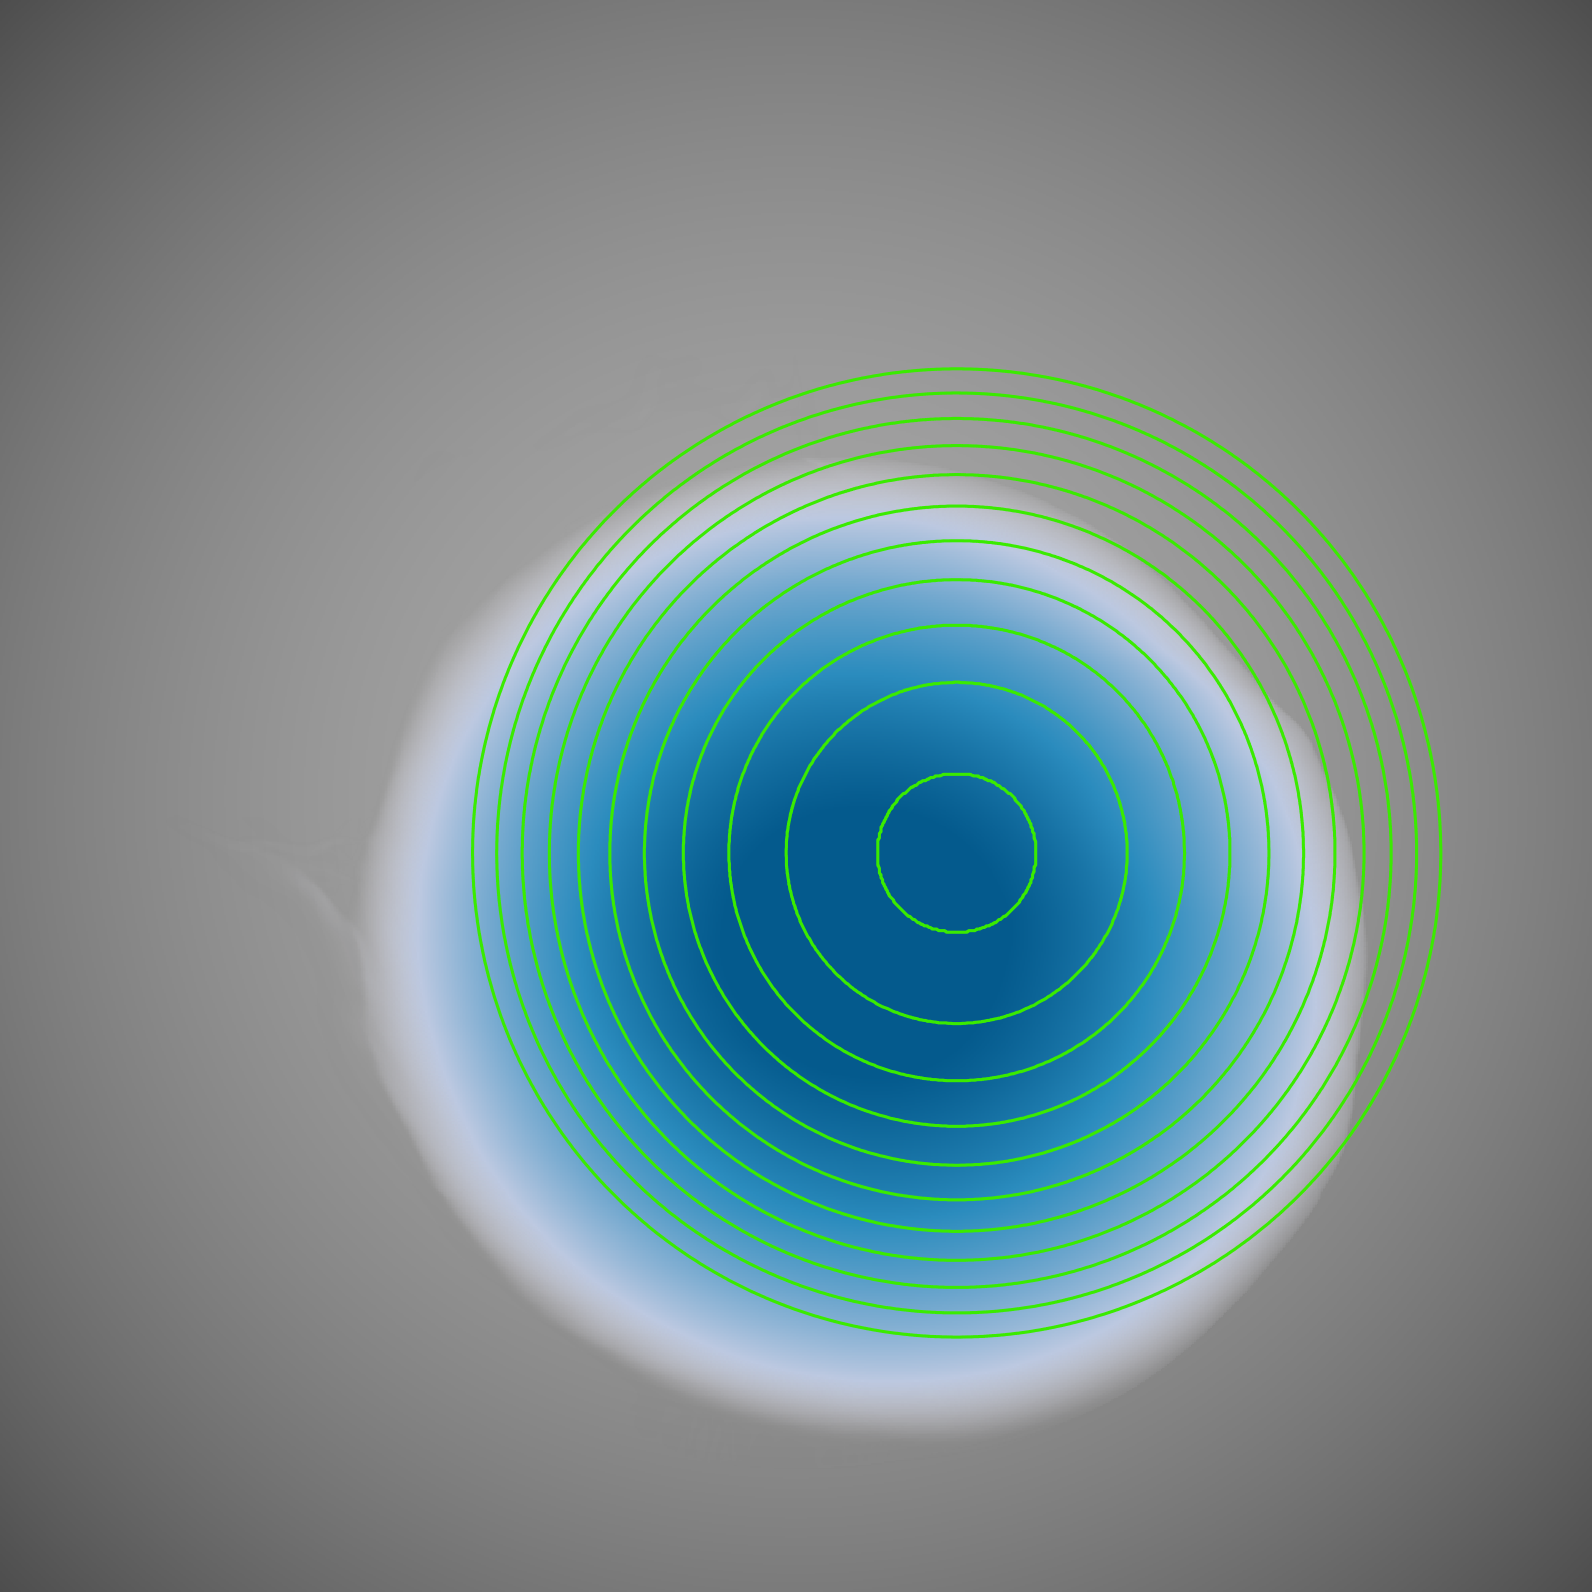
\includegraphics[width=0.4\textwidth]{numerical-test-figures/parabolic-bowl-1O-depth-600s.png} \\
		(a) 300s &
		(b) 600s \\[6pt]
		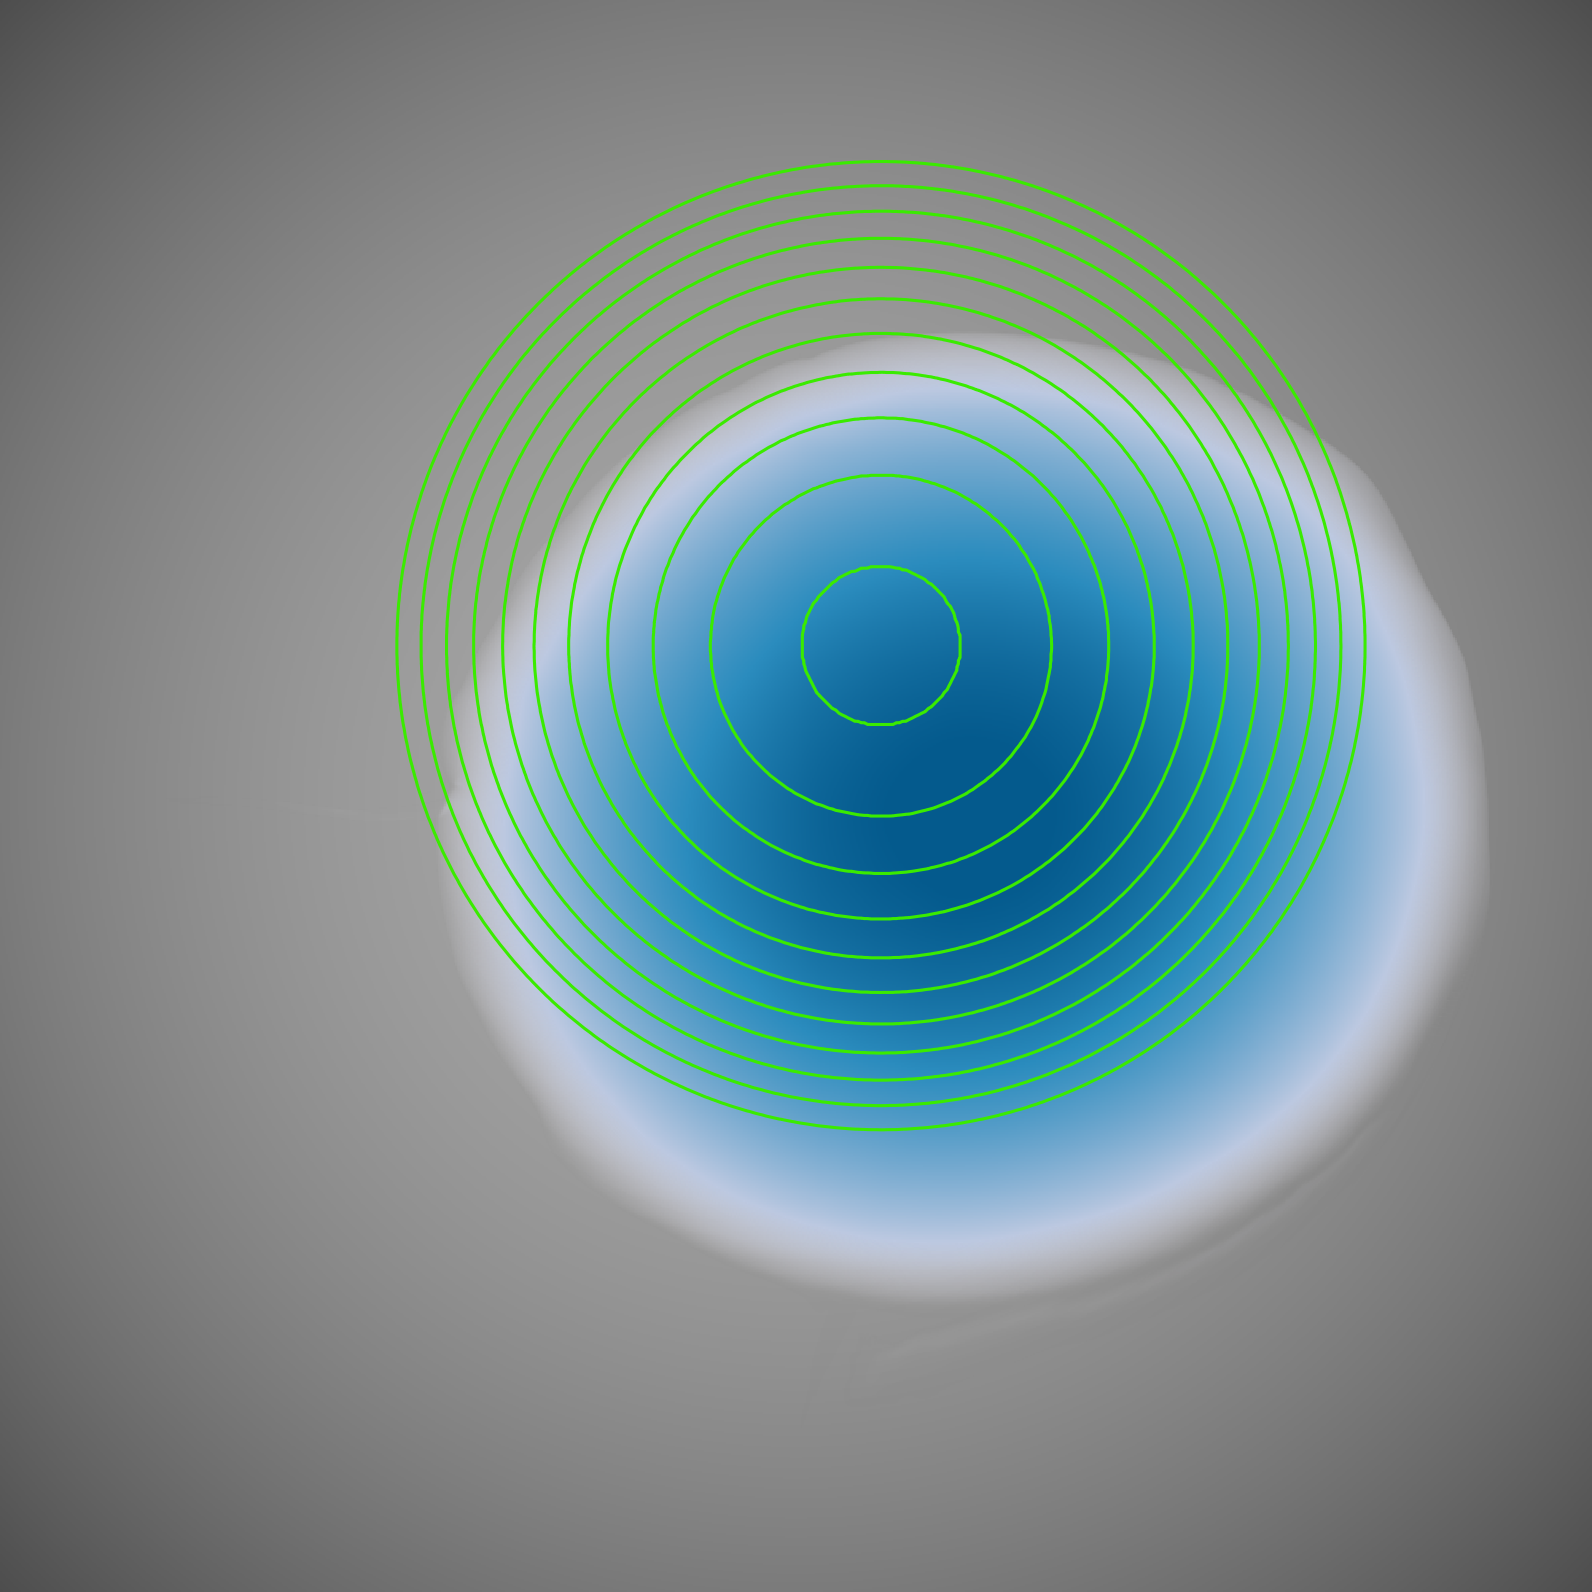
\includegraphics[width=0.4\textwidth]{numerical-test-figures/parabolic-bowl-1O-depth-900s.png} &
		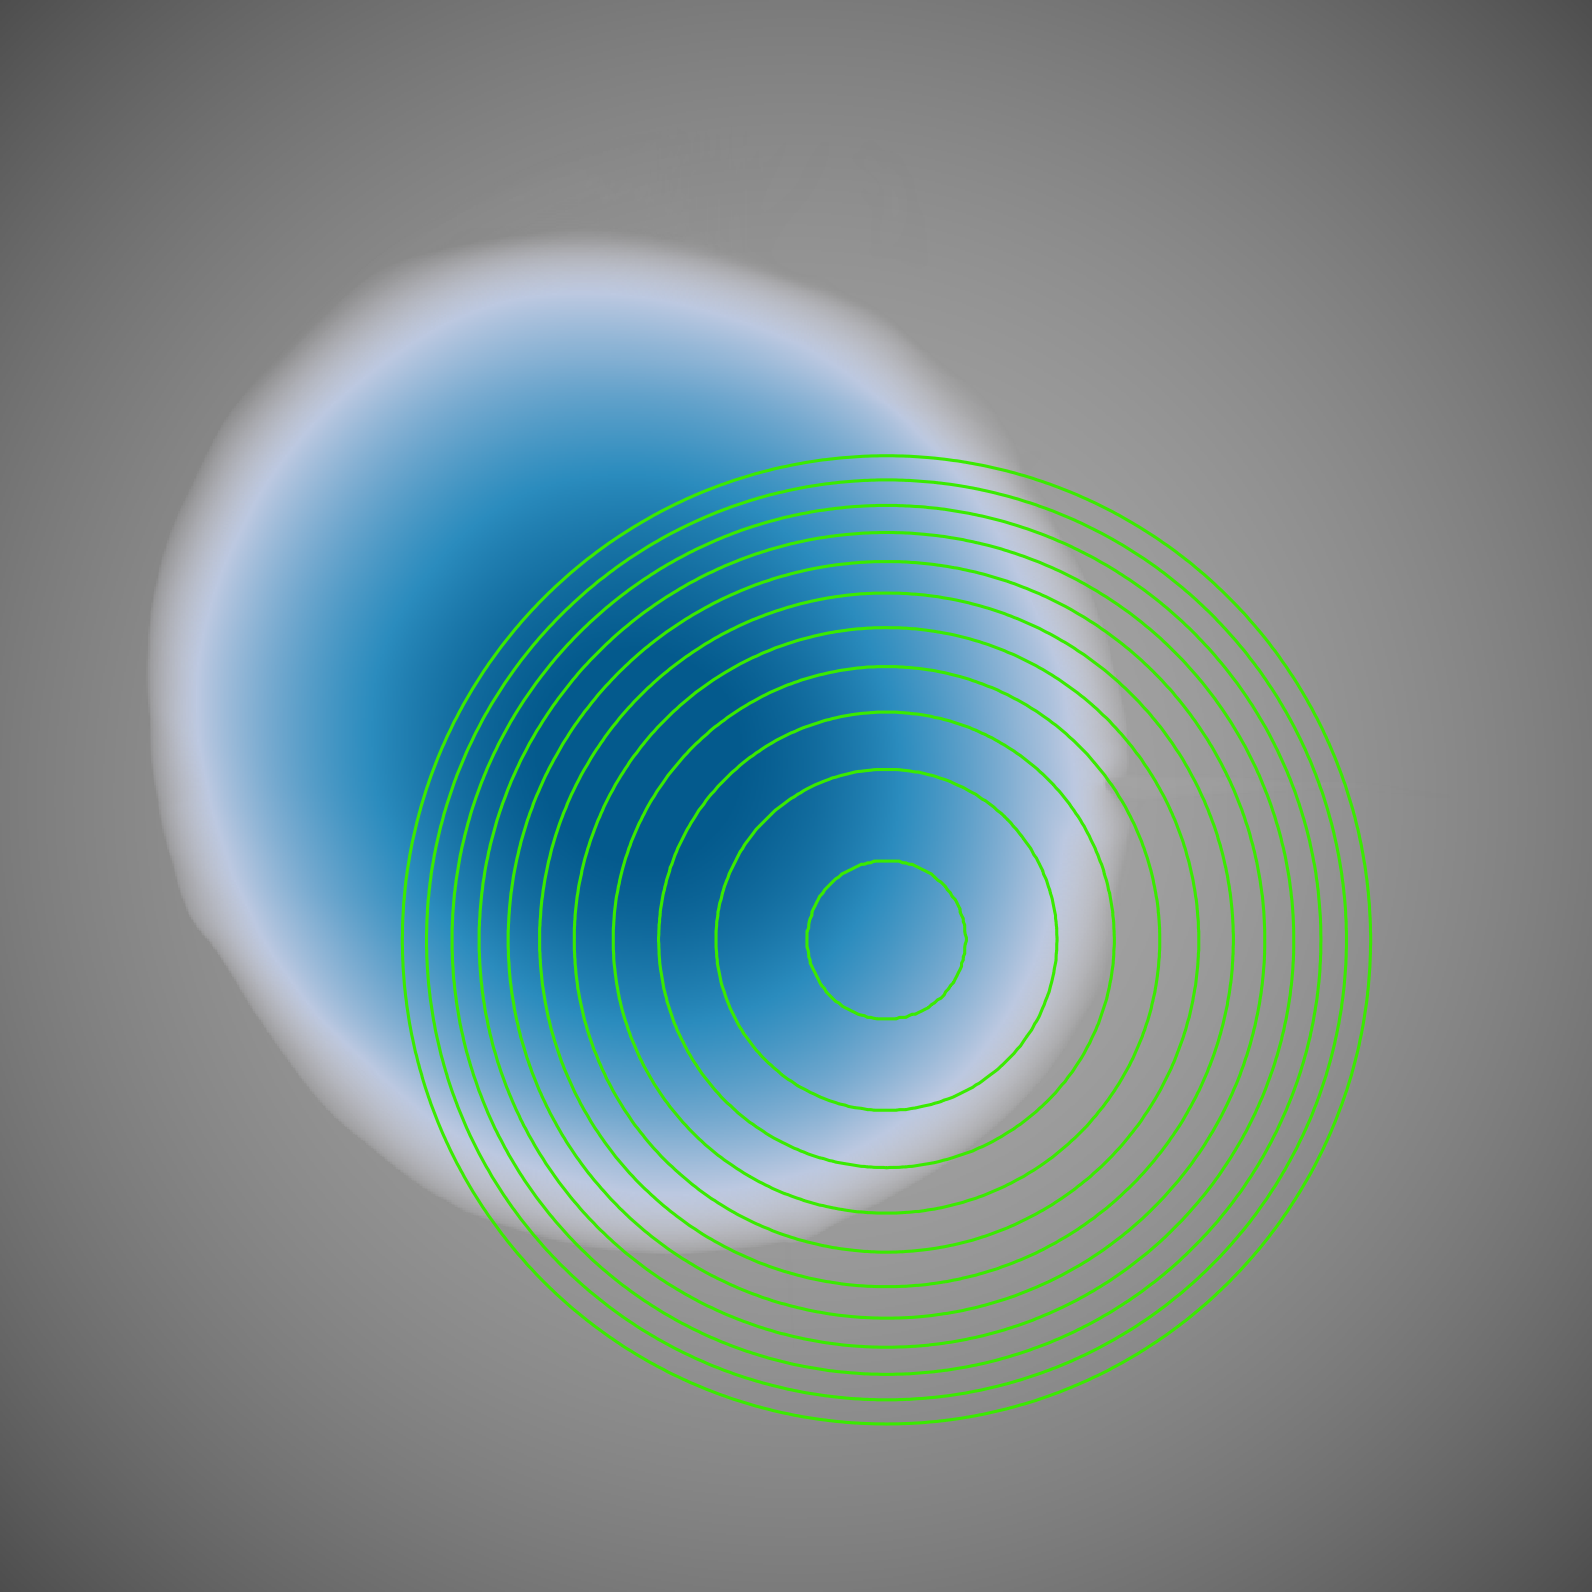
\includegraphics[width=0.4\textwidth]{numerical-test-figures/parabolic-bowl-1O-depth-1800s.png} \\
		(c) 900s &
		(d) 1800s \\[6pt]
		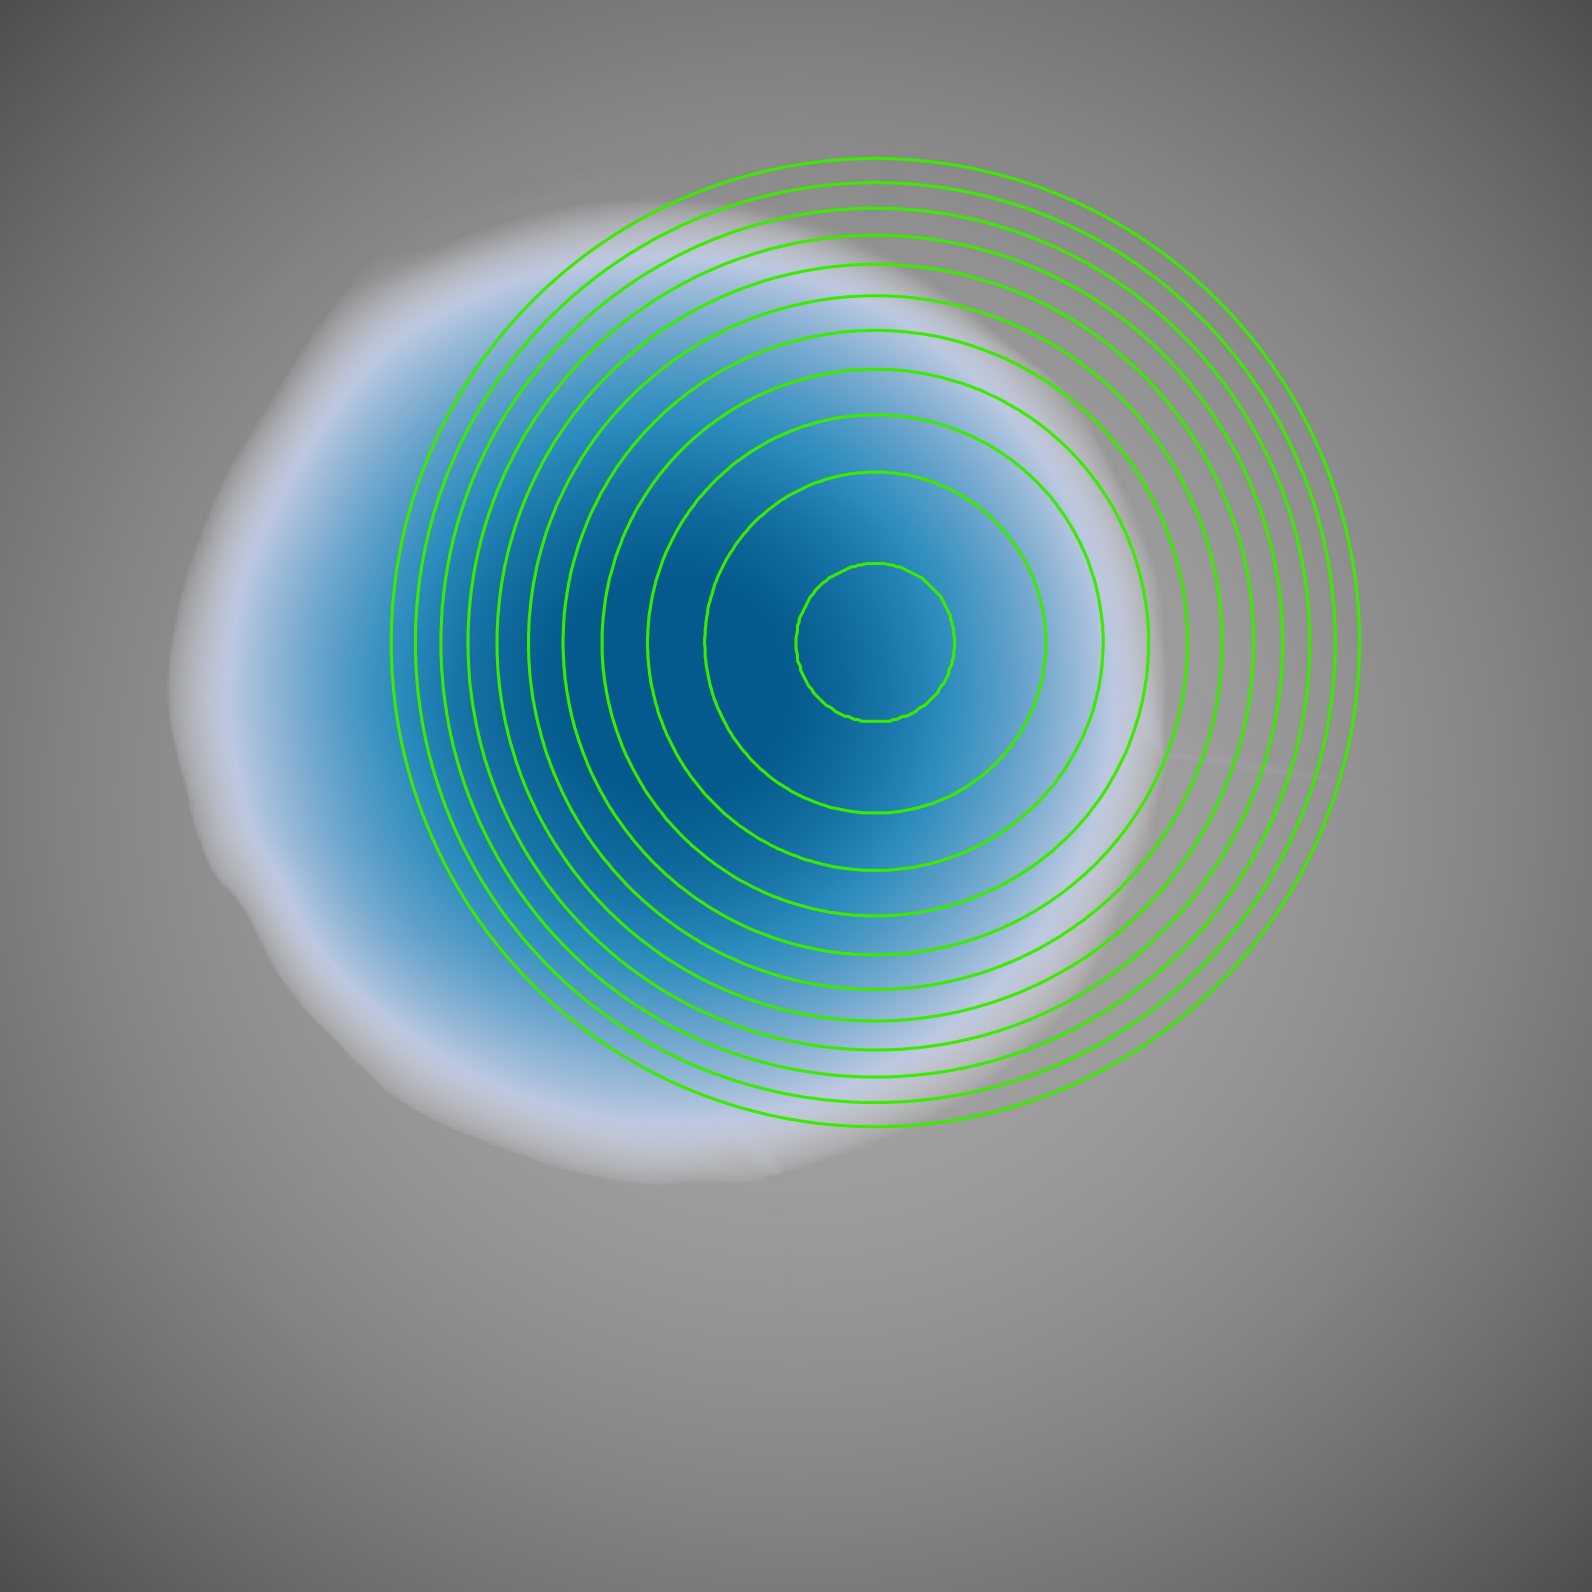
\includegraphics[width=0.4\textwidth]{numerical-test-figures/parabolic-bowl-1O-depth-3600s.png} &
		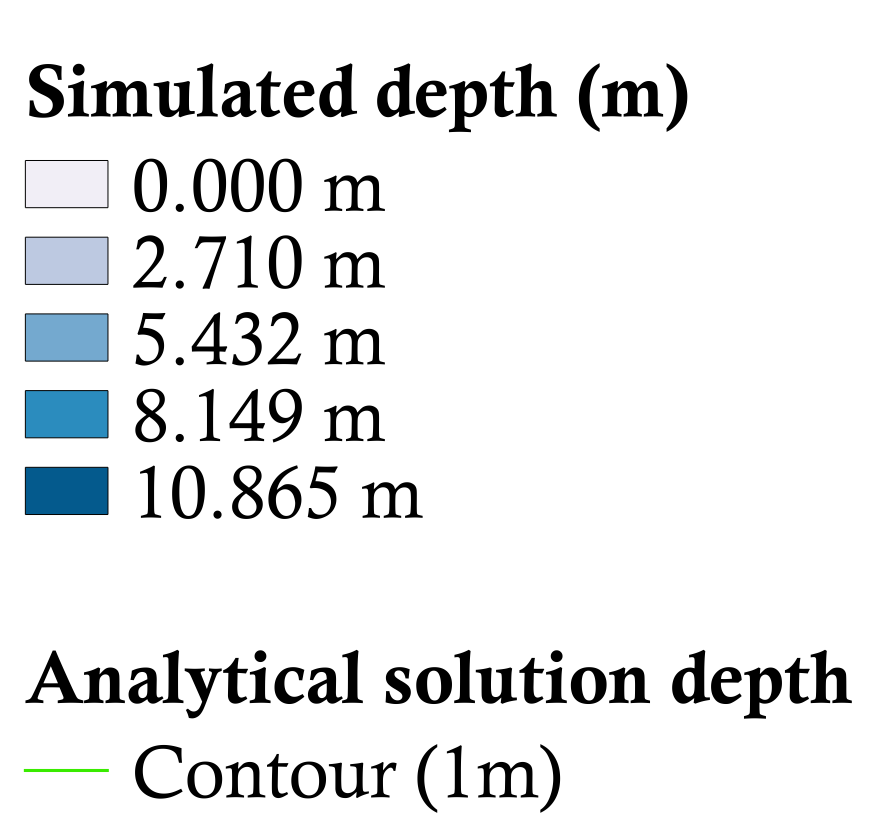
\includegraphics[width=0.26\textwidth]{numerical-test-figures/parabolic-bowl-depth-legend.png} \\
		(e) 3600s &
	\end{tabular}
	\caption{Comparison between analytical solution depth (contours) and simulation results, for first-order solutions.}
	\label{TestResult_ParabolicBowl_1O}
\end{figure*}
\begin{figure*}[tpb]
	\centering
	\begin{tabular}{cc}
		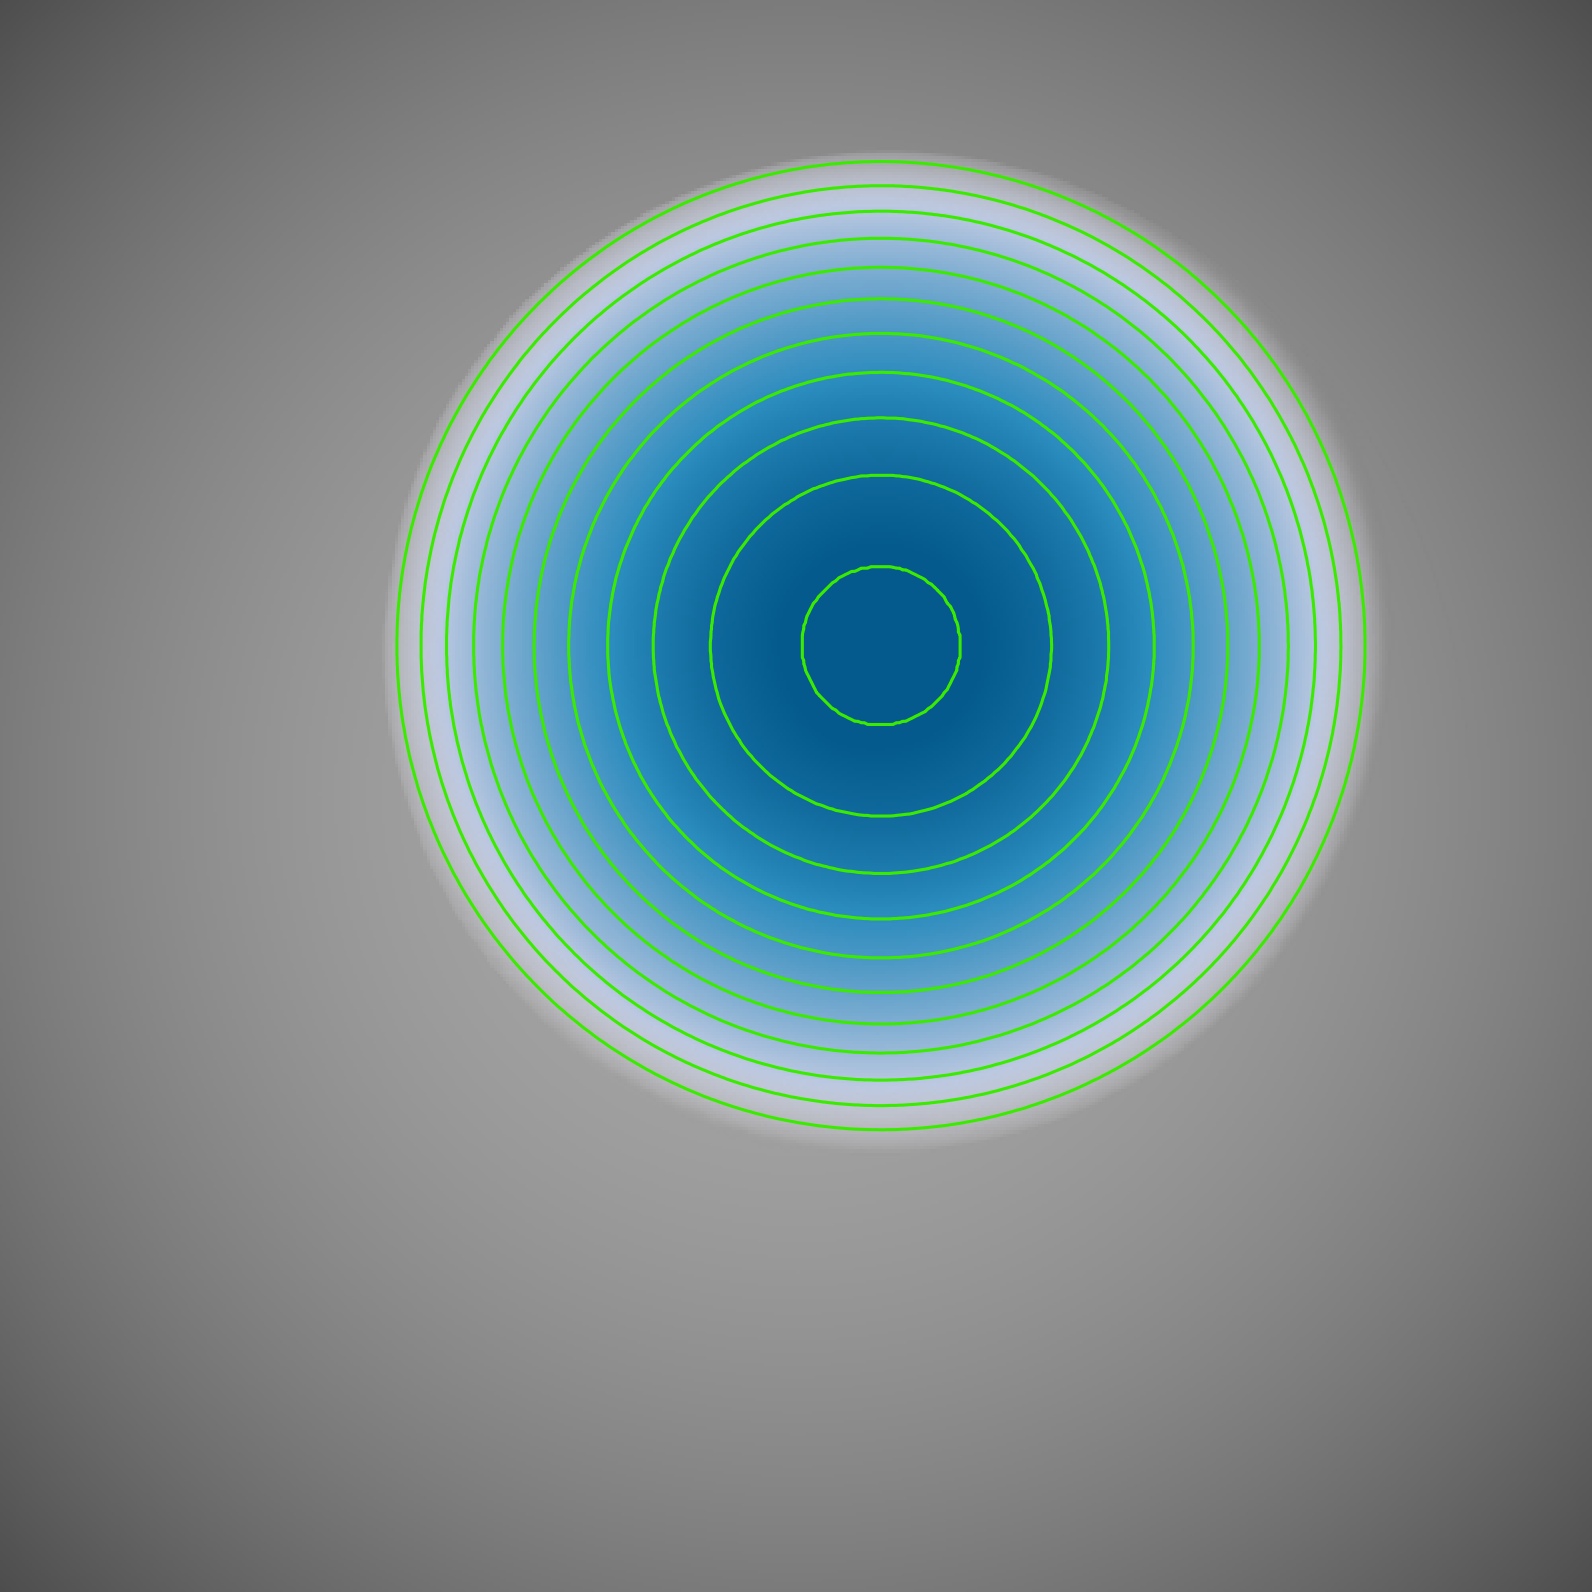
\includegraphics[width=0.4\textwidth]{numerical-test-figures/parabolic-bowl-2O-depth-900s.png} &
		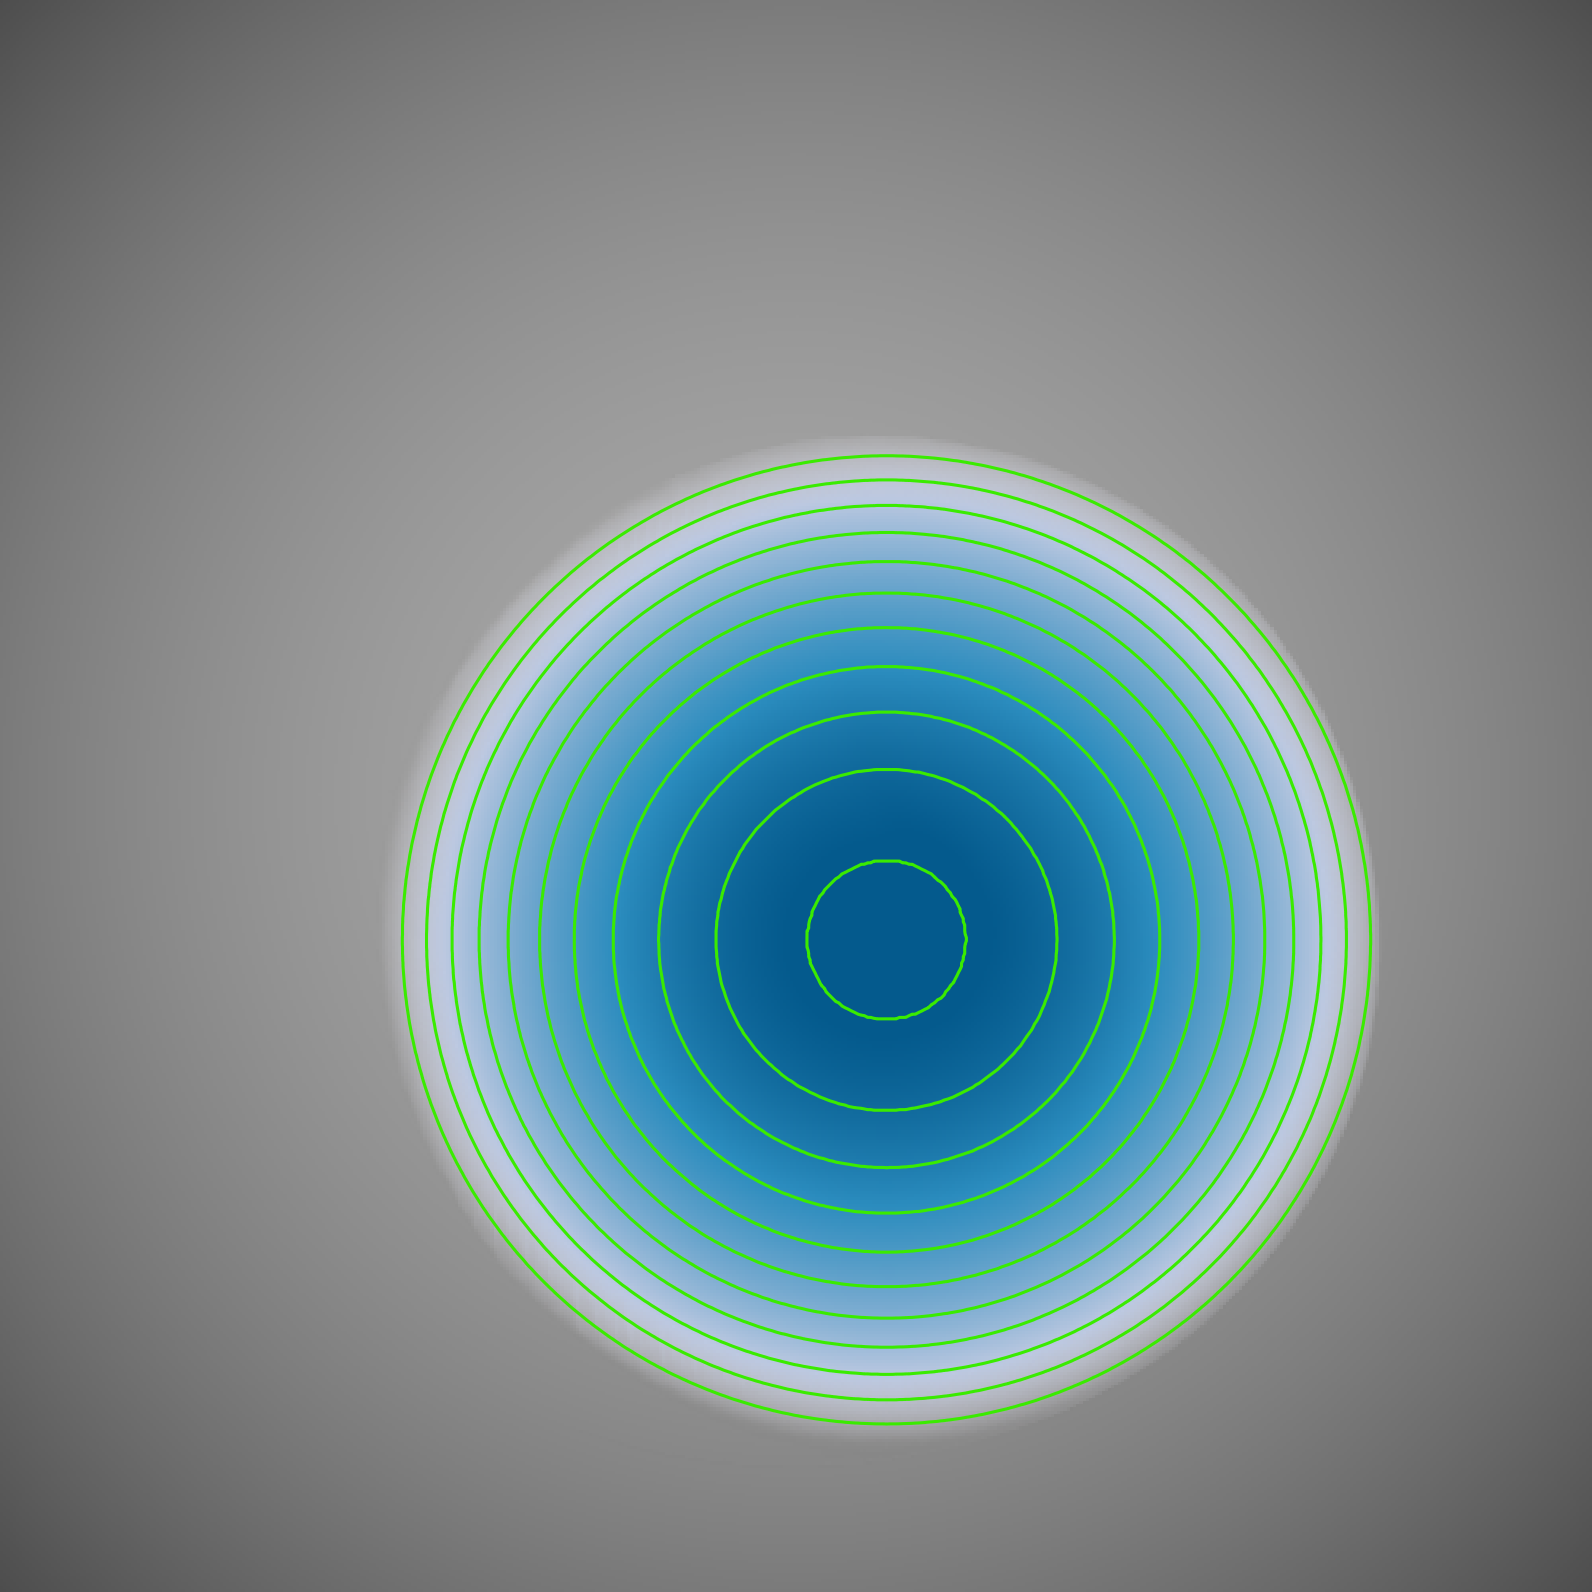
\includegraphics[width=0.4\textwidth]{numerical-test-figures/parabolic-bowl-2O-depth-1800s.png} \\
		(a) 900s &
		(b) 1800s \\[6pt]
		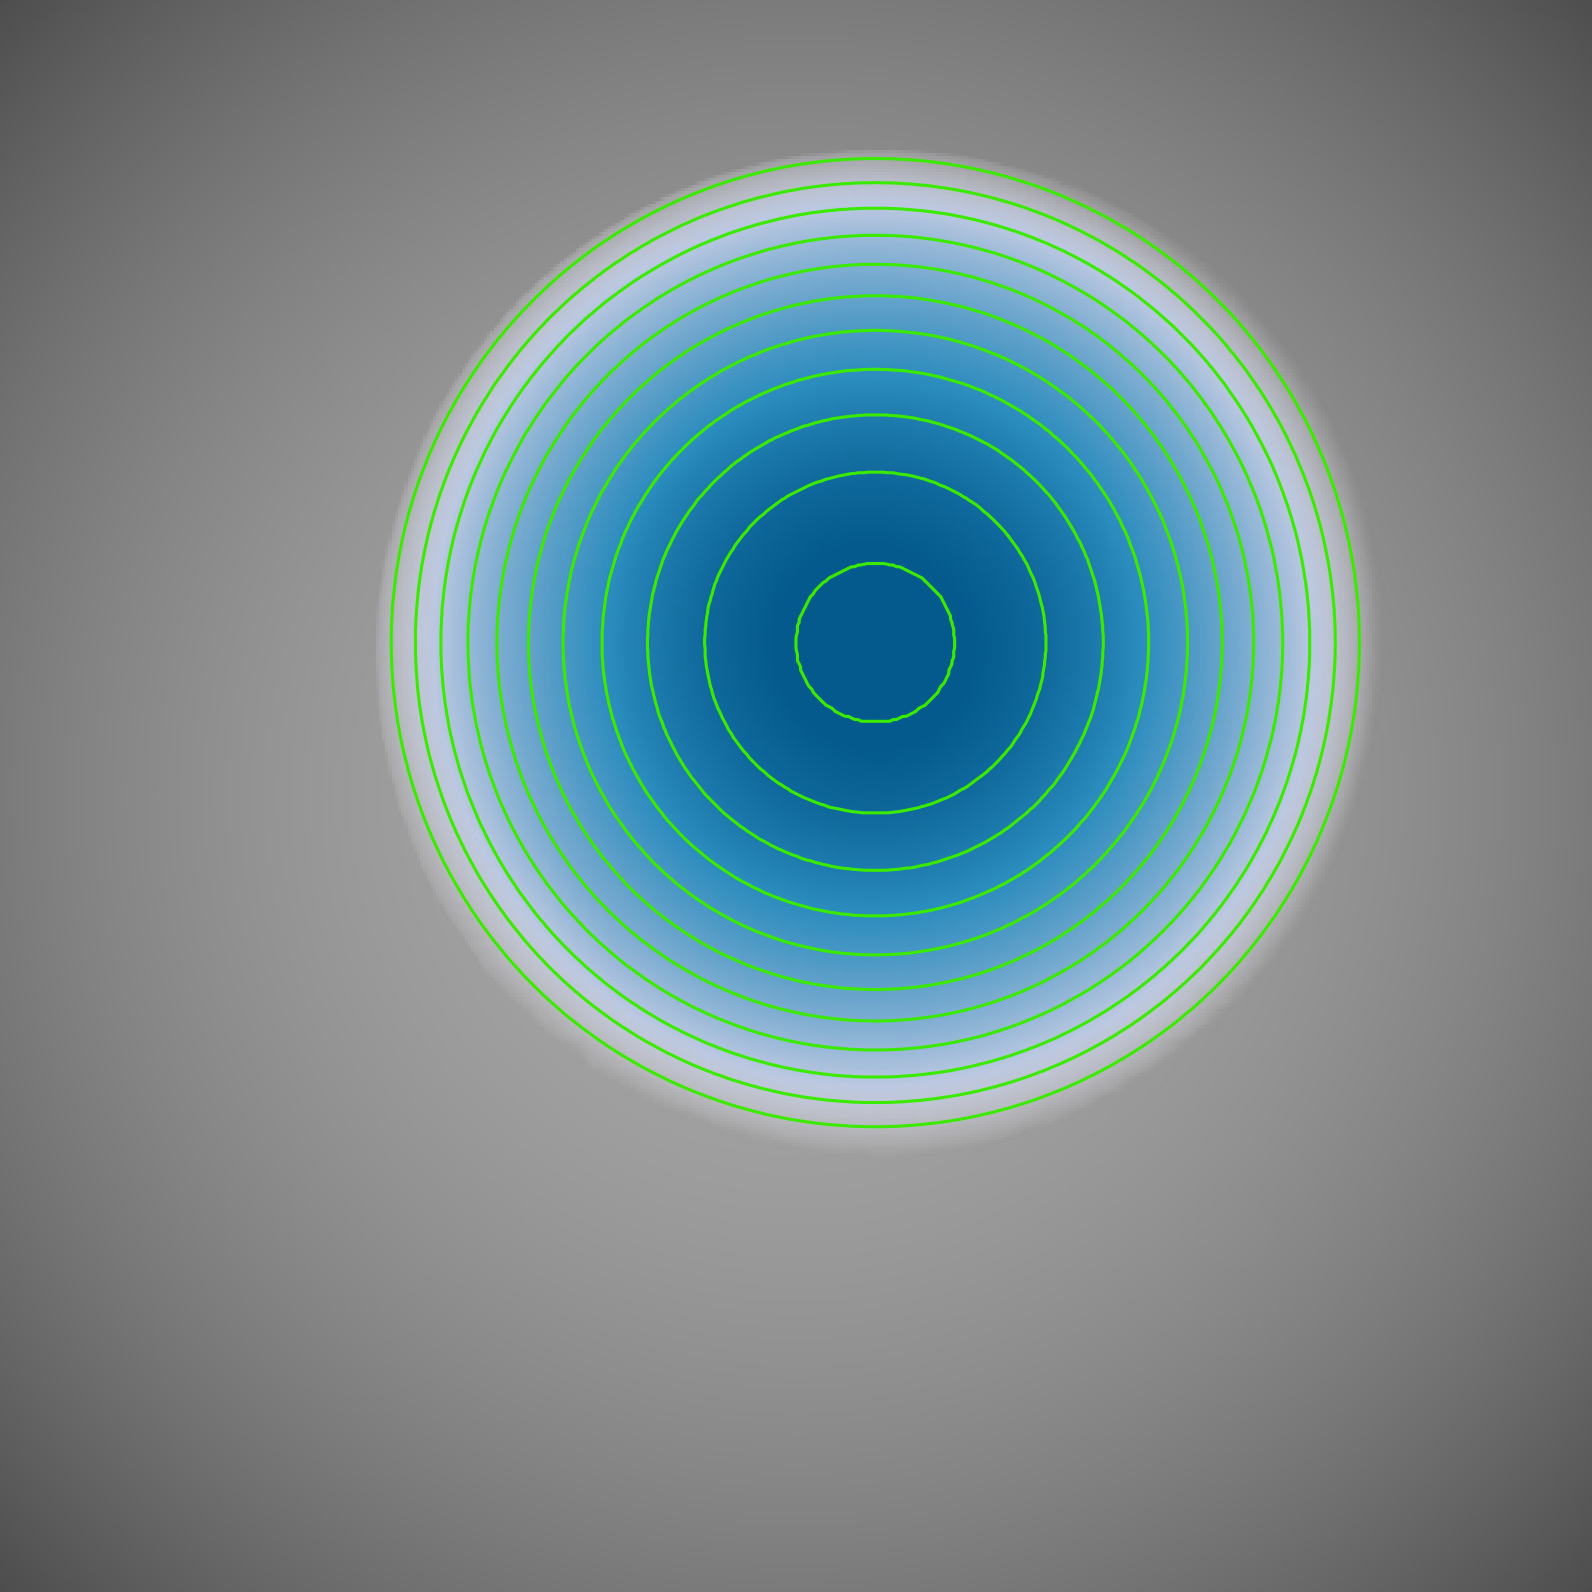
\includegraphics[width=0.4\textwidth]{numerical-test-figures/parabolic-bowl-2O-depth-3600s.png} &
		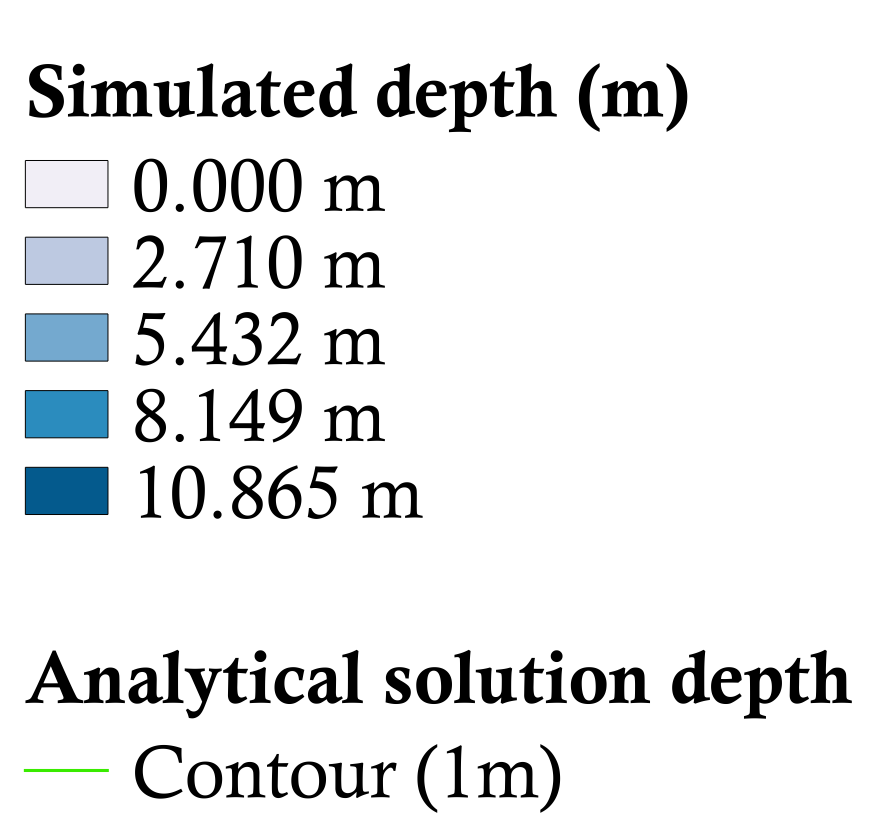
\includegraphics[width=0.26\textwidth]{numerical-test-figures/parabolic-bowl-depth-legend.png} \\
		(c) 3600s &
	\end{tabular}
	\caption{Comparison between analytical solution depth (contours) and simulation results, for second-order solutions.}
	\label{TestResult_ParabolicBowl_2O}
\end{figure*}

Constantly changing wet and dry fronts provide a more challenging situation for the numerical scheme, but are representative of situations arising during pluvial, fluvial, and tidal flooding situations. An analytical solution is known for the case of a parabolic bowl, with water travelling at a velocity around the bowl, and friction neglected such that there is no reduction in velocity with time. A correct solution should theoretically forecast the position of the wet-dry fronts at any point in time, while numerical diffusion is expected to manifest as a gradually increasing deformity in the shape of the flow. Derivation and more comprehensive details for the test case are provided in \citet{Wang2011}.

A scaling factor $h_0 = 10.0$, sloping factor $\alpha = 3000.0$, initial velocity $\beta = 5.0$ and friction parameter of $\tau = 0.0$ are used herein, with the derivative constants,
\begin{equation}
\label{Test_ParabolicBowl_Derivatives}
a = \sqrt{8 g \frac{h_0}{\alpha^2}}, \\
S = \frac{\sqrt{a^2 - \tau^2}}{2}
.
\end{equation}

The initial conditions and analytical results are thus described,
\begin{equation}
\label{Test_ParabolicBowl_Conditions}
\begin{alignedat}{2}
z_b & = h_0 \frac{x^2 + y^2}{\alpha^2}, \\
\eta & = h_0 - \frac{1}{g} \beta e^{\displaystyle-\frac{\tau t}{2}} \times \left( \frac{\tau}{2} sin(St) + S cos(St) \right) x \\
& - \frac{1}{g} \beta e^{\displaystyle-\frac{\tau t}{2}} \times \left( \frac{\tau}{2} cos(St) + S sin(St) \right) y, \\
u & = \beta e^{\displaystyle-\frac{\tau t}{2}} sin(St), \\
v & = -\beta e^{\displaystyle-\frac{\tau t}{2}} cos(St),
\end{alignedat}
\end{equation}
where $t = 0.0$ for initial conditions.

Results for the first-order case at different time periods are presented in Figure \ref{TestResult_ParabolicBowl_1O}. A correct solution has the analytical result overlapping the simulation, whereas it is clearly visible that the error grows as time passes. This is a consequence of numerical dispersion. The overall behaviour however is nonetheless represented correctly. 

A similar figure is provided for the results of a second-order MUSCL-Hancock simulation in Figure \ref{TestResult_ParabolicBowl_2O}, where despite the numerical scheme's requirement to fall back to first-order solutions along wet-dry fronts, to the advantage of numerical stability, the overall simulation result matches almost exactly with the analytical solution.

\section{Dam-break simulation over an emerging bed}

The results provided so far in this chapter, have not sufficiently tested the numerical scheme's capability for capturing the behaviour of shocks, encompassing hydraulic jump phenomena, and other such complexities encountered in the real world. The failure of a dam, in which water rapidly leaves a body of water with considerable depth, creates high velocities and may result in a hydraulic jump. A theoretical dam break over an emerging bed is therefore considered, whereby the inclined bed removes energy from the oncoming wave. A wall is provided around the extremity of the domain, such as to contain the flow, and with a thickness of two cells thereby ensuring all cells which will become inundated are included in the computational domain, with respect to the earlier discussions on cell data requirements in first- and second-order solutions. This is an adaptation of the example employed by \citet{Xing2010}.

Only the MUSCL-Hancock scheme is employed, as the most appropriate scheme for the flow under consideration. No friction effects are considered.

The initial conditions and domain are described as,
\begin{equation}
\label{Test_EmergingBed_Conditions}
\begin{alignedat}{4}
z_b & = x \cdot tan(\theta) &&, \\
u & = 0.0, && \\
v & = 0.0, && \\
d & = \eta && where \hspace{1cm} x < p,
\end{alignedat}
\end{equation}
where constants are $\displaystyle\theta = \frac{\pi}{60}, \eta = 1.0, p = 0.0$. The domain is considered to be 30.00m in length, 0.35m in width, and represented by 4,200 cells of resolution 0.05m, with the grid origin in the centre of the domain. This provides sufficient room for the shock and rarefaction waves to propagate without encountering the extremity of the domain for the first few seconds.

\begin{sidewaysfigure}
	\centering
	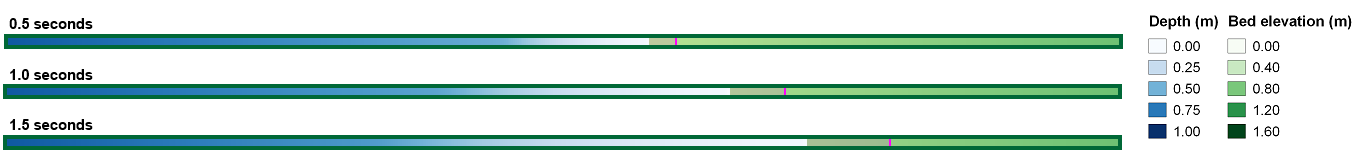
\includegraphics[width=1.05\textheight]{numerical-test-figures/dam-break-emerging-bed-example.png}
	\caption{Comparison between the inundated area in simulation results, and the analytical solution for the position of the front (shown as a line), for the dam-break against an emerging bed test.}
	\label{TestResult_EmergingBed}
\end{sidewaysfigure}

The position of the front is determined by,
\begin{equation}
\label{Test_EmergingBed_FrontPosition}
x_{front} = 2t \sqrt{g h_0 cos(\theta)} - \frac{gt^2 \cdot tan(\theta)}{2},
\end{equation} and shown against the simulation results in Figure \ref{TestResult_EmergingBed}.

The limitations of the numerical methods and modelling employed are clear in the results, with the simulated front progressively further from the analytically-derived front. In this case, especially against the adverse gradient of the domain, it is possible that the second-order method falling back to first-order at the wet-dry front is not sufficiently alleviating the numerical diffusion effects. Moreover, it is also worth considering, that the scheme employed is two-dimensional and relies upon depth-averaged velocities and shallow water assumptions, as discussed in the comparative study of \citet{Liang2010}. The author does not believe these results to be of particular concern, especially considering that the correct behaviour is exhibited by the simulation, and the likelihood that  limitations observed would likely require extension to three dimensions, and considerably more complex and expensive numerical methods, to achieve any significant improvement in the results. 

\section{Dam-break against a fixed obstacle}

\begin{sidewaysfigure}
	\centering
	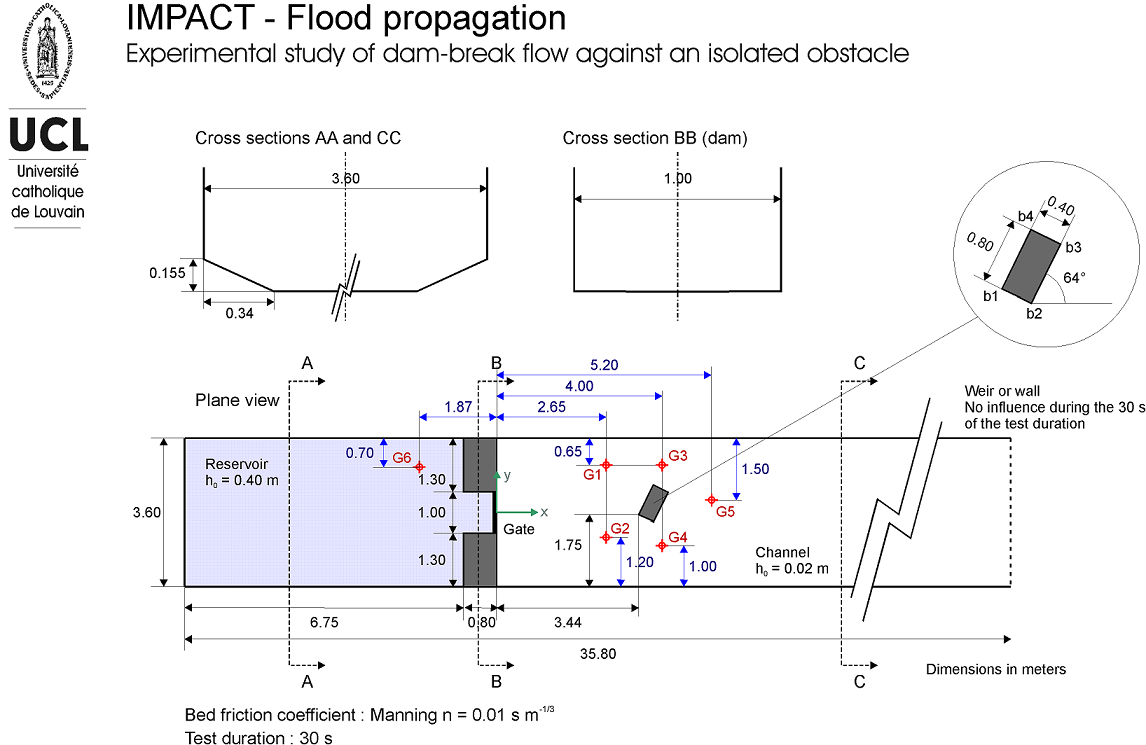
\includegraphics[width=1.0\textwidth]{numerical-test-figures/dam-break-obstacle-layout.png}
	\caption{Layout for the dam-break against an obstacle, showing the position of the gauges, position of the grid origin, and location of the obstacle.}
	\label{TestResult_DamObstacle_Domain}
\end{sidewaysfigure}

A dam-break against an obstacle presents a more complex situation again, for which there is no analytical solution. In practice, any dam failure would undoubtedly result in flow against obstacles, hence this is a useful test. A laboratory study conducted as part of the IMPACT project provides measurements and sufficient data to reproduce the situation in a simulation \citep{SoaresFrazao2007}. The dimensions of the domain and locations of gauges are shown in Figure \ref{TestResult_DamObstacle_Domain}, which is represented by a 0.02m grid, hence 322,200 cells in total.

The complex interaction between the shock and rarefaction waves, and those reflected from the obstacle are shown in the simulation results after three seconds (Figure \ref{TestResult_DamObstacle_Depth}), in a pattern and manner consistent with those described by \citet{SoaresFrazao2007}, clearly showing areas of supercritical flow.

A comparison between gauge measurements and simulation results is given in Figure \ref{TestResult_DamObstacle_Gauges}, where the simulation clearly exhibits the correct behaviour, even if the exact measurements show discrepancies. The arrival of wave-fronts appears delayed in comparison to the observations, and is often followed by exaggerated levels upon arrival. This is likely to be a consequence of the limitations of the shallow water equations during the initial dam-break, which may be underestimating the initial velocity of the wave-front.

\begin{sidewaysfigure}
	\centering
	\begin{subfigure}{1.0\textheight}
	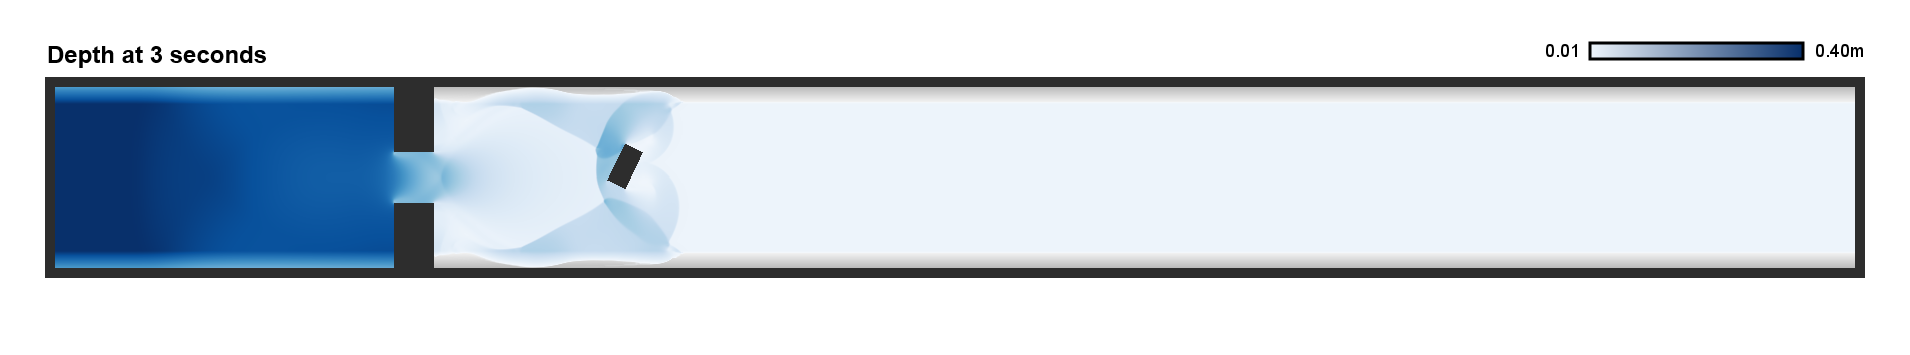
\includegraphics[width=1.0\textheight]{numerical-test-figures/dam-break-obstacle-depth-example.png}
	\caption{Depth, where darker colours are deeper, after a three second period.}
	\label{TestResult_DamObstacle_Depth}
	\end{subfigure}
	\begin{subfigure}{1.0\textheight}
	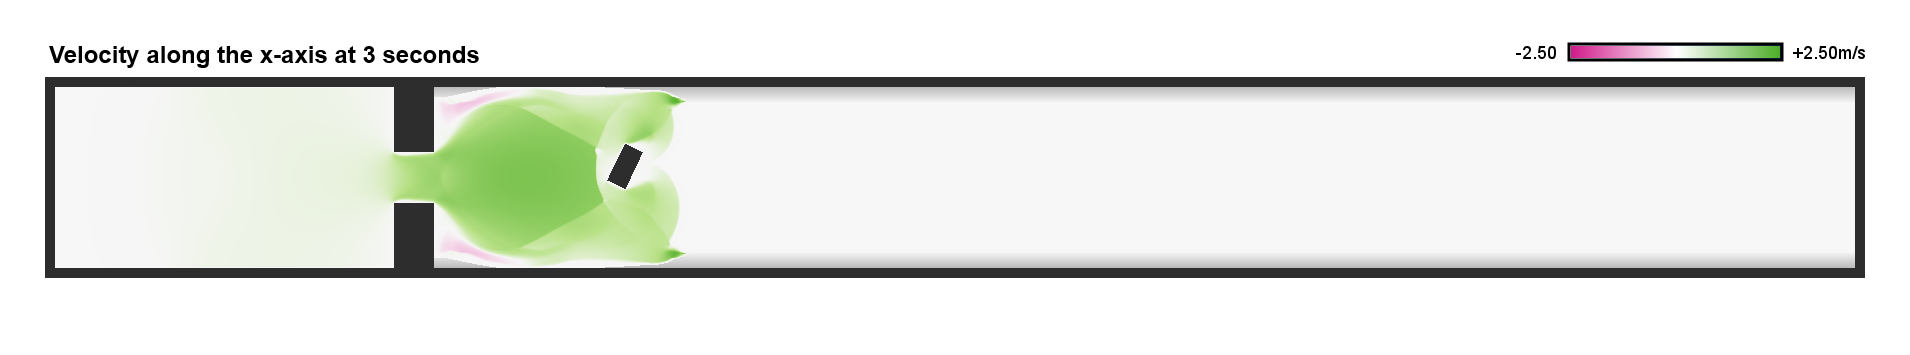
\includegraphics[width=1.0\textheight]{numerical-test-figures/dam-break-obstacle-velocity-example.png}
	\caption{Velocity, along $x$-axis where darker colours are higher, after a three second period.}
	\label{TestResult_DamObstacle_Velocity}
	\end{subfigure}
	\caption{Representation of depth and velocity in the dam break against an obstacle.}
\end{sidewaysfigure}
\begin{figure*}[tpb]
	\centering
	\begin{tabular}{cc}
		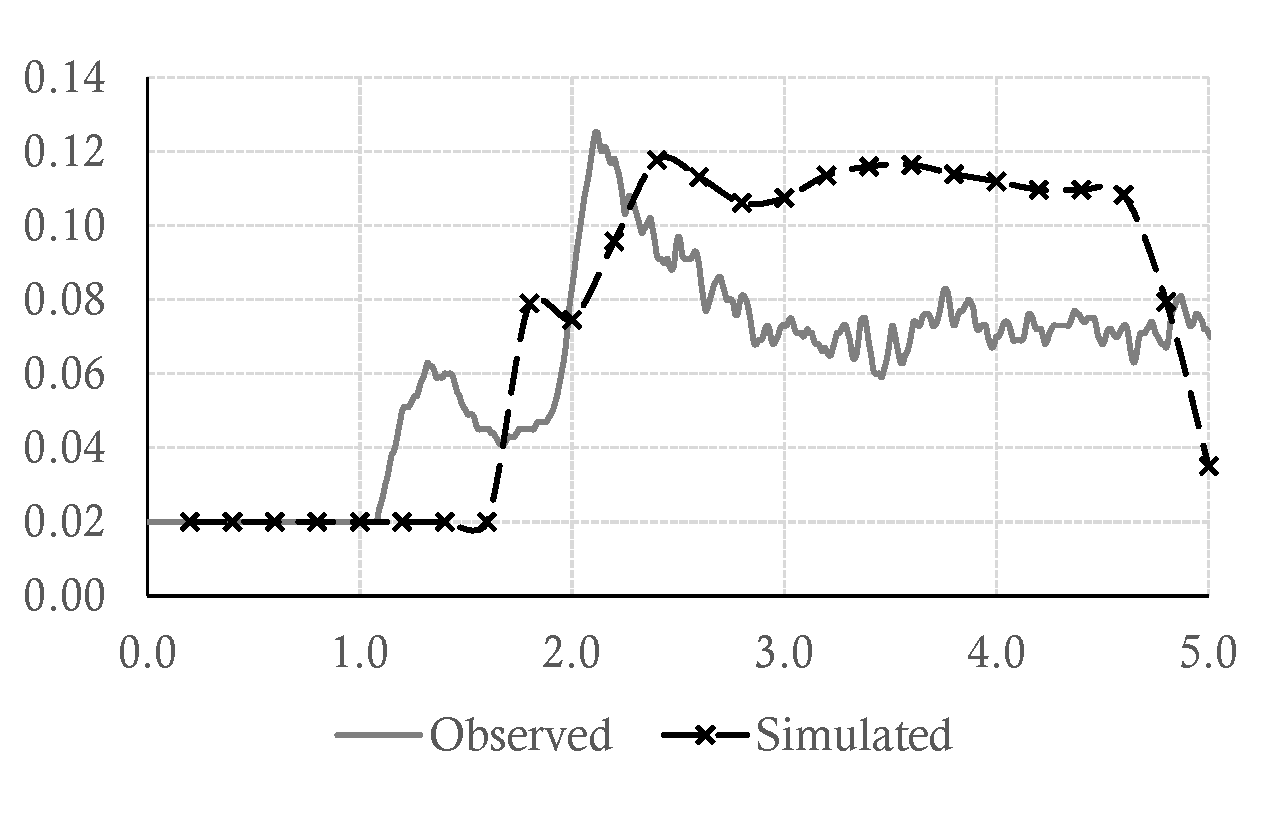
\includegraphics[width=0.5\textwidth]{numerical-test-figures/dam-break-obstacle-results-g1.pdf} &
		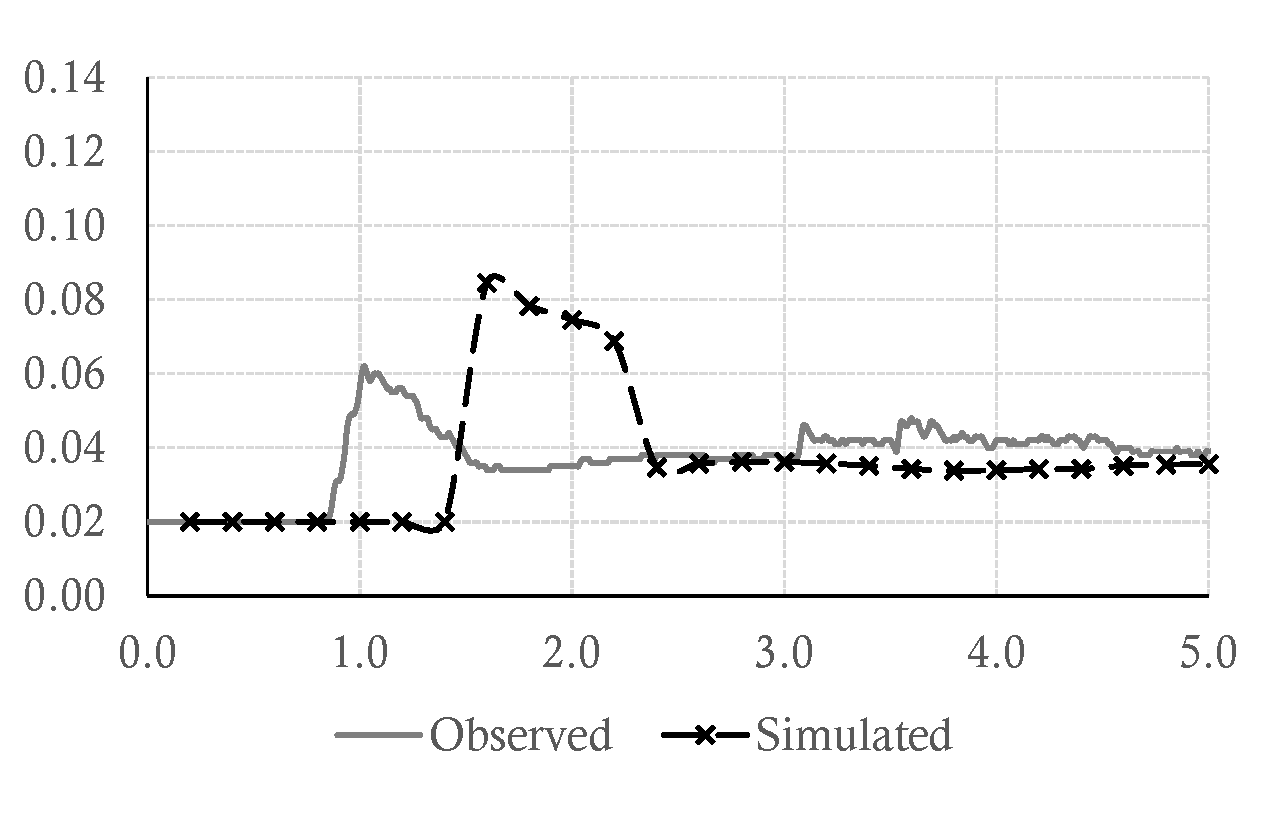
\includegraphics[width=0.5\textwidth]{numerical-test-figures/dam-break-obstacle-results-g2.pdf} \\
		(a) G1 &
		(b) G2 \\[6pt]
		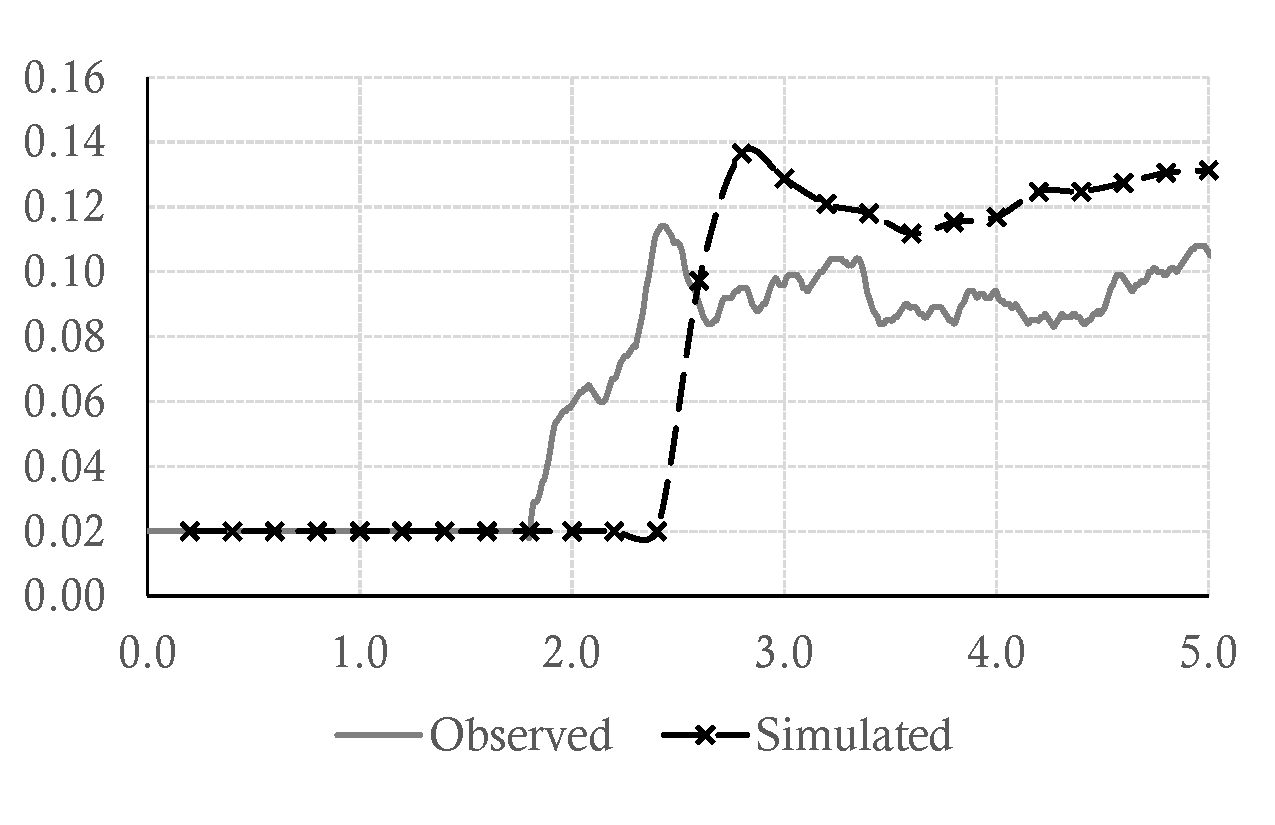
\includegraphics[width=0.5\textwidth]{numerical-test-figures/dam-break-obstacle-results-g3.pdf} &
		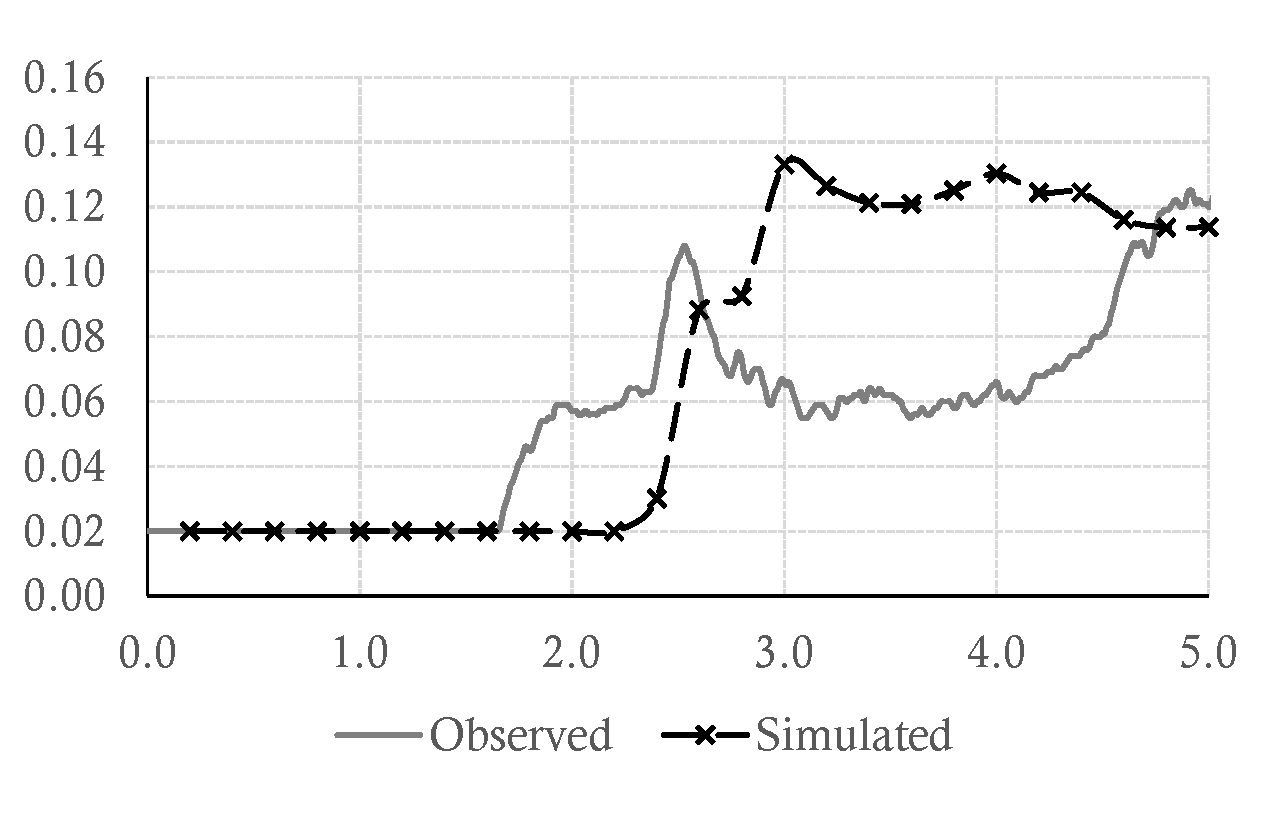
\includegraphics[width=0.5\textwidth]{numerical-test-figures/dam-break-obstacle-results-g4.pdf} \\
		(c) G3 &
		(d) G4 \\[6pt]
		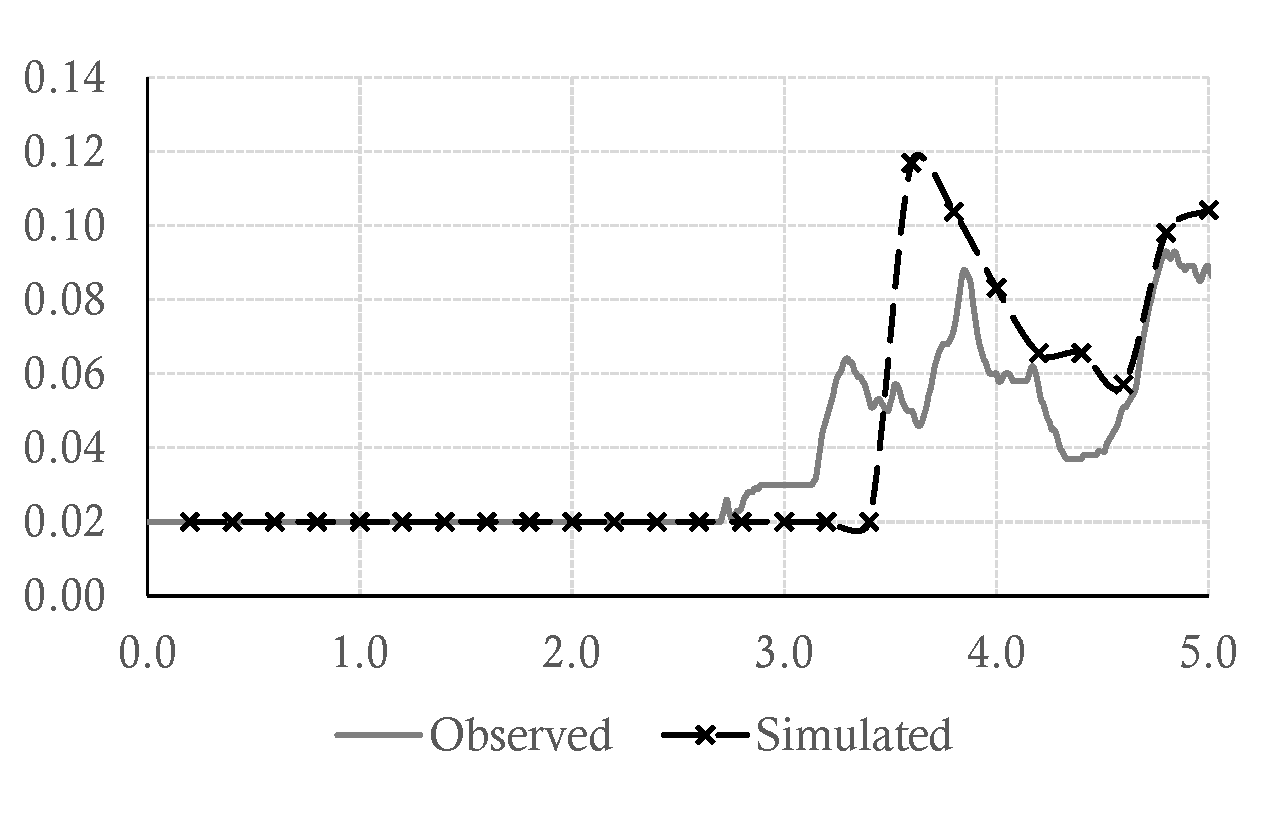
\includegraphics[width=0.5\textwidth]{numerical-test-figures/dam-break-obstacle-results-g5.pdf} &
		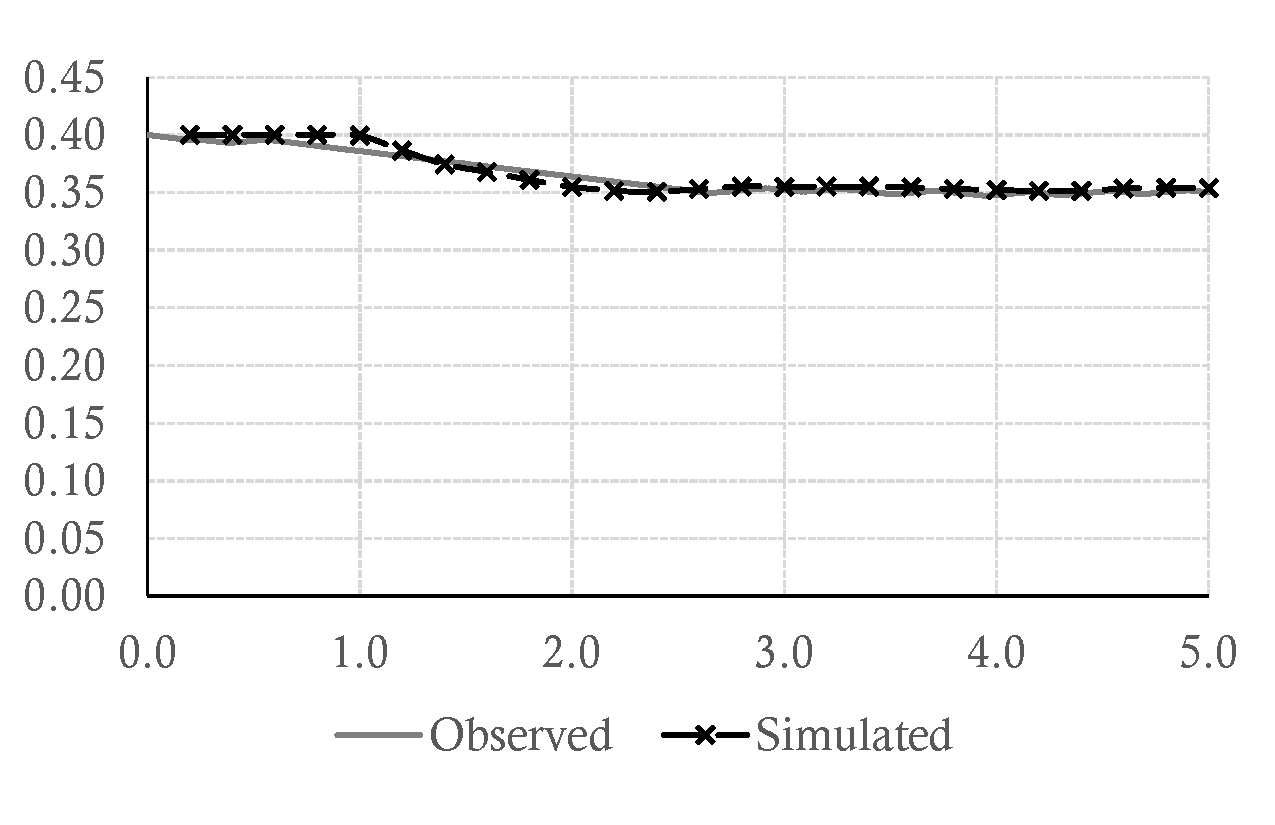
\includegraphics[width=0.5\textwidth]{numerical-test-figures/dam-break-obstacle-results-g6.pdf} \\
		(e) G5 &
		(f) G6 \\
	\end{tabular}
	\caption{Depth comparison between laboratory gauges and simulated results during the first five seconds.}
	\label{TestResult_DamObstacle_Gauges}
\end{figure*}

\section{Hypothetical pluvial flood event}

The previous results provided suggest second-order solutions are required in a wide variety of cases, to avoid significant deviations from the correct result as a consequence of numerical diffusion. Herein, a realistic scenario is considered, of a hypothetical pluvial flood event caused by intense rainfall, within a real-world domain.

The UK Environment Agency commissions a report periodically examining the differences in results, suitability and performance of different 2D hydraulic modelling packages. One of the more complex test-cases therein is a short hypothetical flood event occurring as a combination of both a point inflow and uniform precipitation in the area surrounding Cockenzie Street, Glasgow. The test was performed in accordance with \citet{Pender2010} and \citet{Pender2013}, simulating a 5-hour period.

The inflow hydrograph and hyetograph are given in Figure \ref{Glasgow_Inflows}. The digital terrain model (DTM) is shown in Figure \ref{Glasgow_DTM} alongside the location of the point inflow at (264896, 664747). Data was supplied at 0.5m resolution but has been resampled to 2m to allow comparison with published results for other software. The computational domain contains 97,083 cells. A uniform Manning coefficient of 0.05 is used everywhere except for roads and pavements where a value of 0.02 is assigned, to allow direct comparison with the results in \citet{Pender2010}, although it should be recognised each software will implement the treatment of Manning's $n$ in slightly different manners, hence this is a source of uncertainty. Closed boundary conditions are applied around the extremity of the domain. The surcharging sewer hydrograph is implemented by direct addition of volume to the cell, hence with no initial velocity.

\begin{figure*}[tpb]
\centering
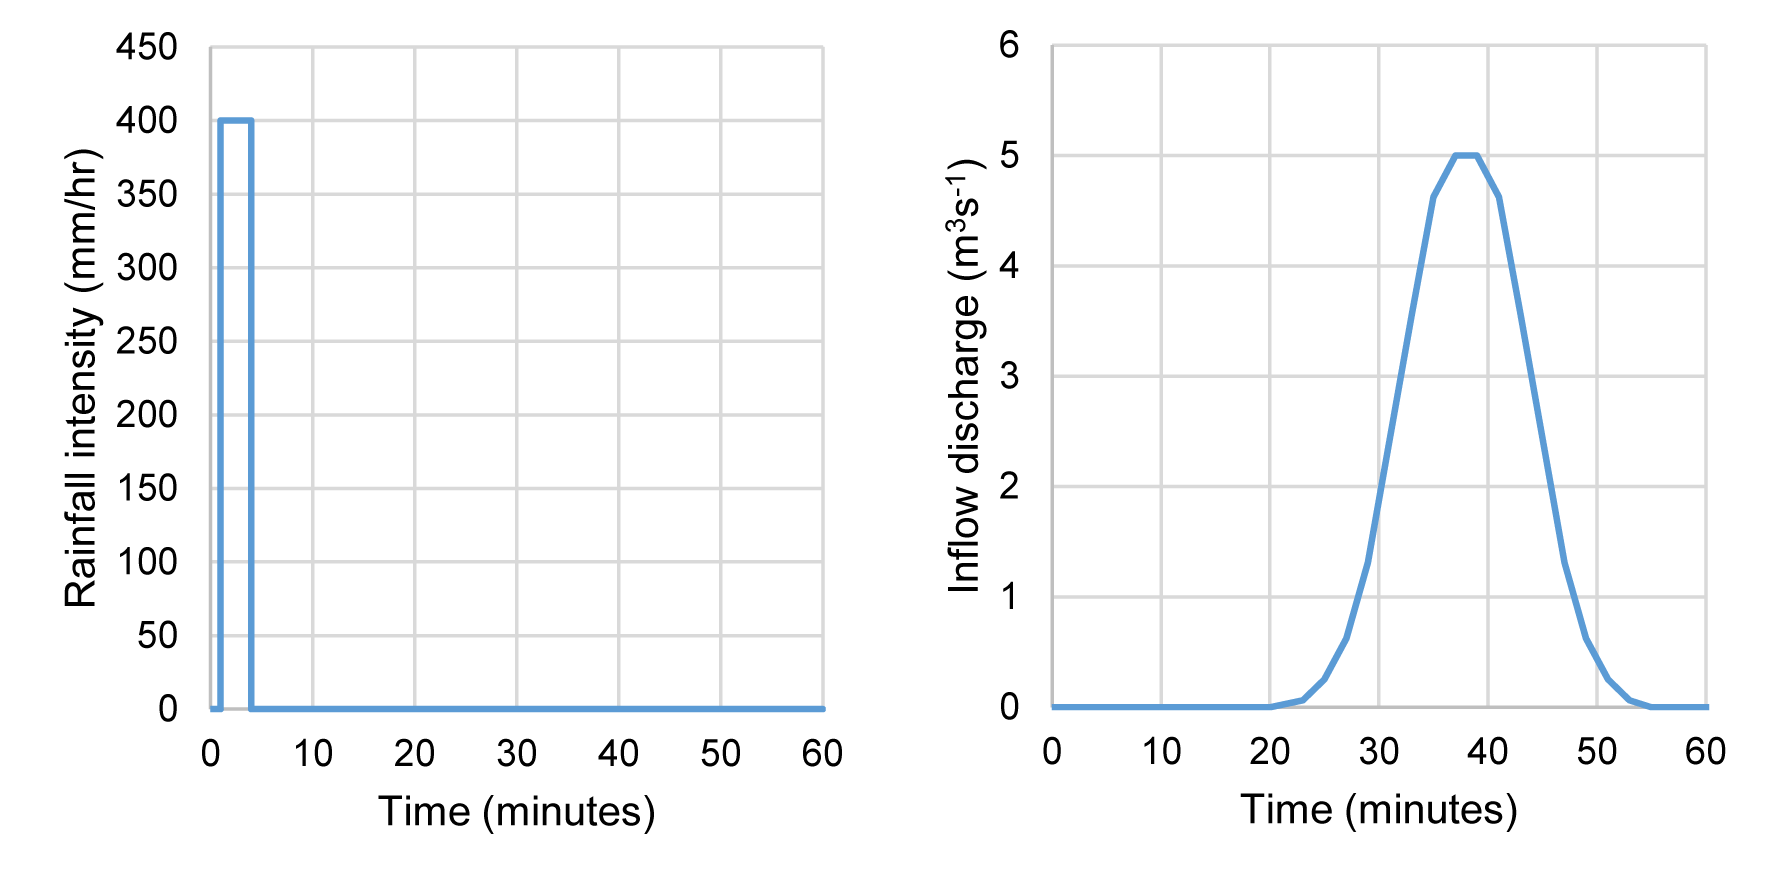
\includegraphics[width=0.75\textwidth]{heterogeneous-dev-figures/Glasgow_Inflow.png}
\caption{Boundary conditions for Glasgow test: (a) Uniformly distributed rainfall hyetograph; (b) volumetric discharge at the inflow point.}
\label{Glasgow_Inflows}
\end{figure*}
\begin{figure*}[tpb]
\centering
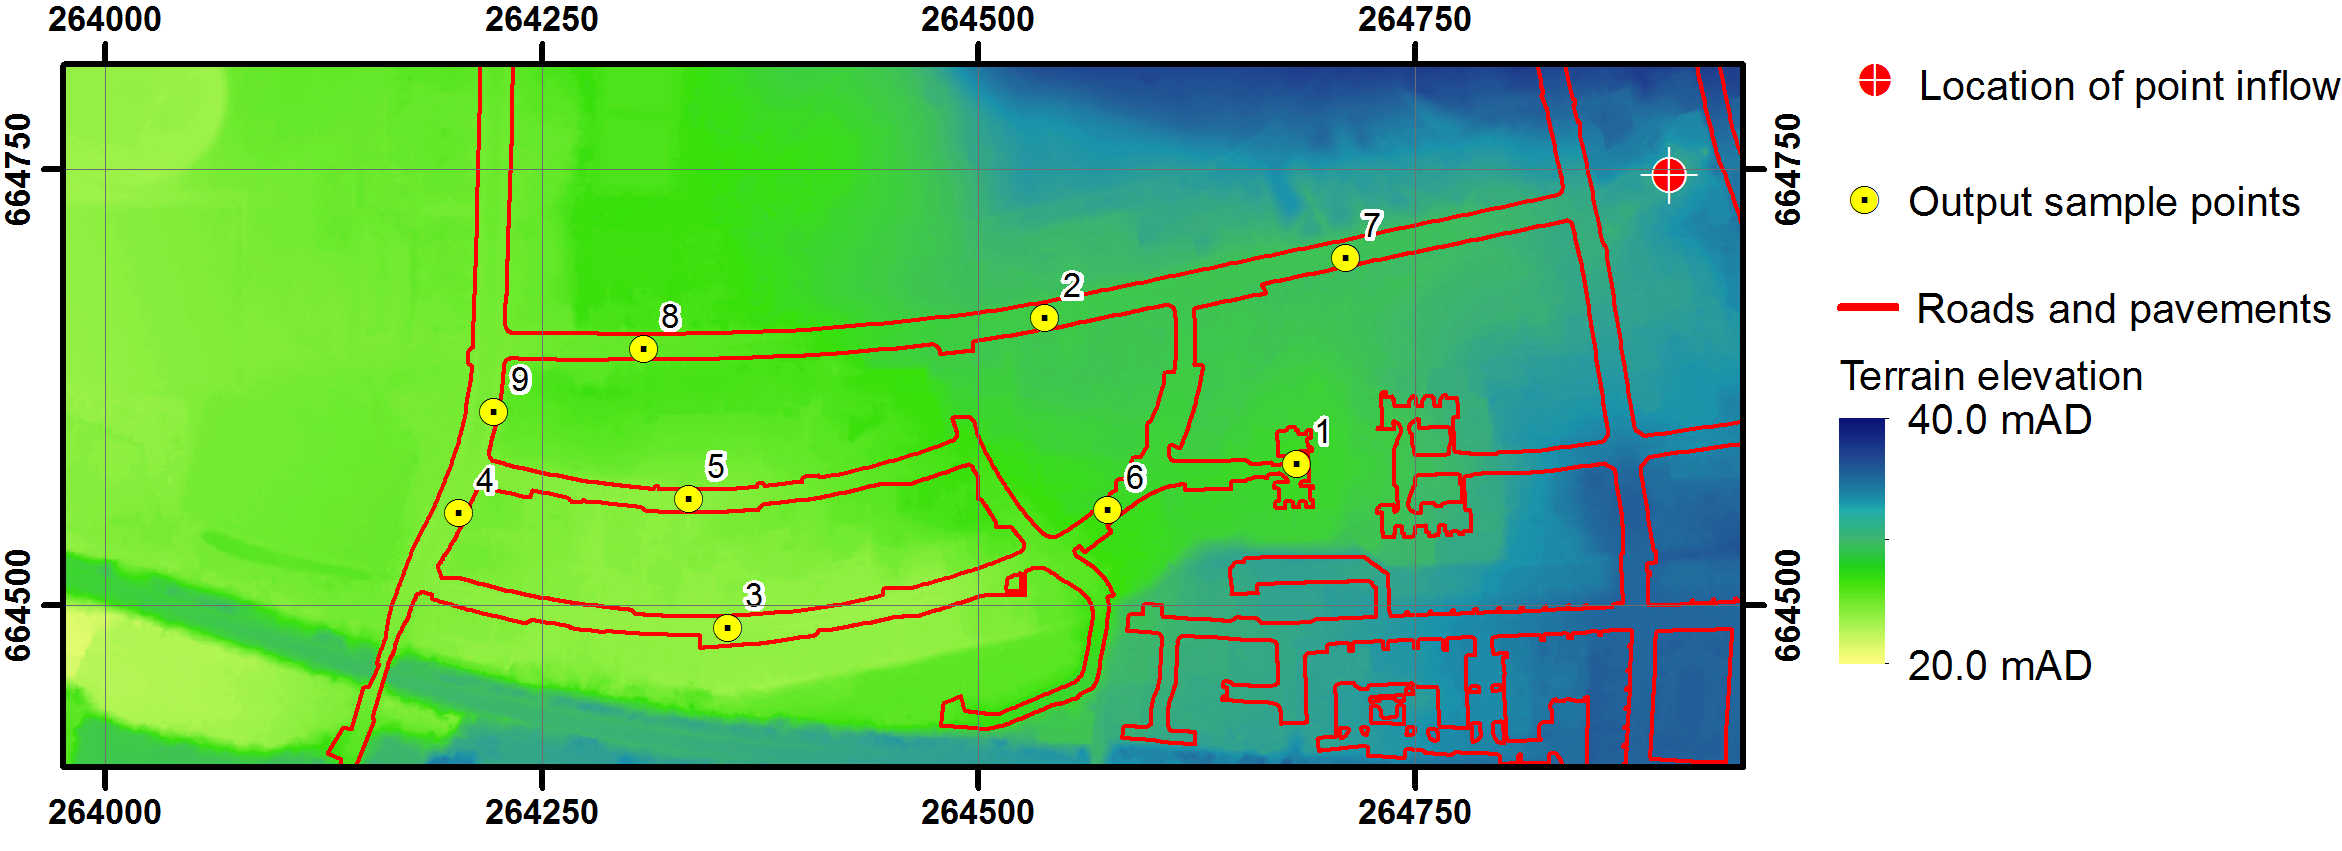
\includegraphics[width=1.0\textwidth]{heterogeneous-dev-figures/Glasgow_DTM.png}
\caption{The surface elevation for a 0.39 km$^{2}$ area of Glasgow with the inflow location indicated and the position of 9 output sample points.}
\label{Glasgow_DTM}
\end{figure*}

Simulations were carried out using 32- and 64-bit floating-point arithmetic (i.e. single- and double-precision). 32-bit arithmetic introduced significant errors (in mass conservation and thus the overall result) for the given numerical scheme, and resulted in timesteps of approximately 0.1s. This is believed to be caused by the lack of numerical resolution for the small depths by which unit-width discharge is divided to give velocities. The typical timestep with 64-bit arithmetic is approximately 0.3s. This difference largely negates the performance benefits that are normally achievable with reduced precision arithmetic for both GPUs and CPUs, and furthermore has implications for any other simulations in which extremely shallow flows might be expected. Results presented hereafter are for 64-bit simulations except where indicated.

The maximum depths recorded per cell at the end of the simulation are displayed in Figure \ref{Glasgow_MaxDepths} at 0.2m intervals. In addition water levels and velocities were output at 9 different points; levels are shown in Figure \ref{Glasgow_PointGraphs} while velocities are omitted for brevity. The maximum depths and timeseries data are consistent with results produced by other software, and close to those of other finite-volume software packages in particular. Small differences are discernible but all fall within the ranges of results presented in \citet{Pender2010}.

\begin{figure*}[tpb]
\centering
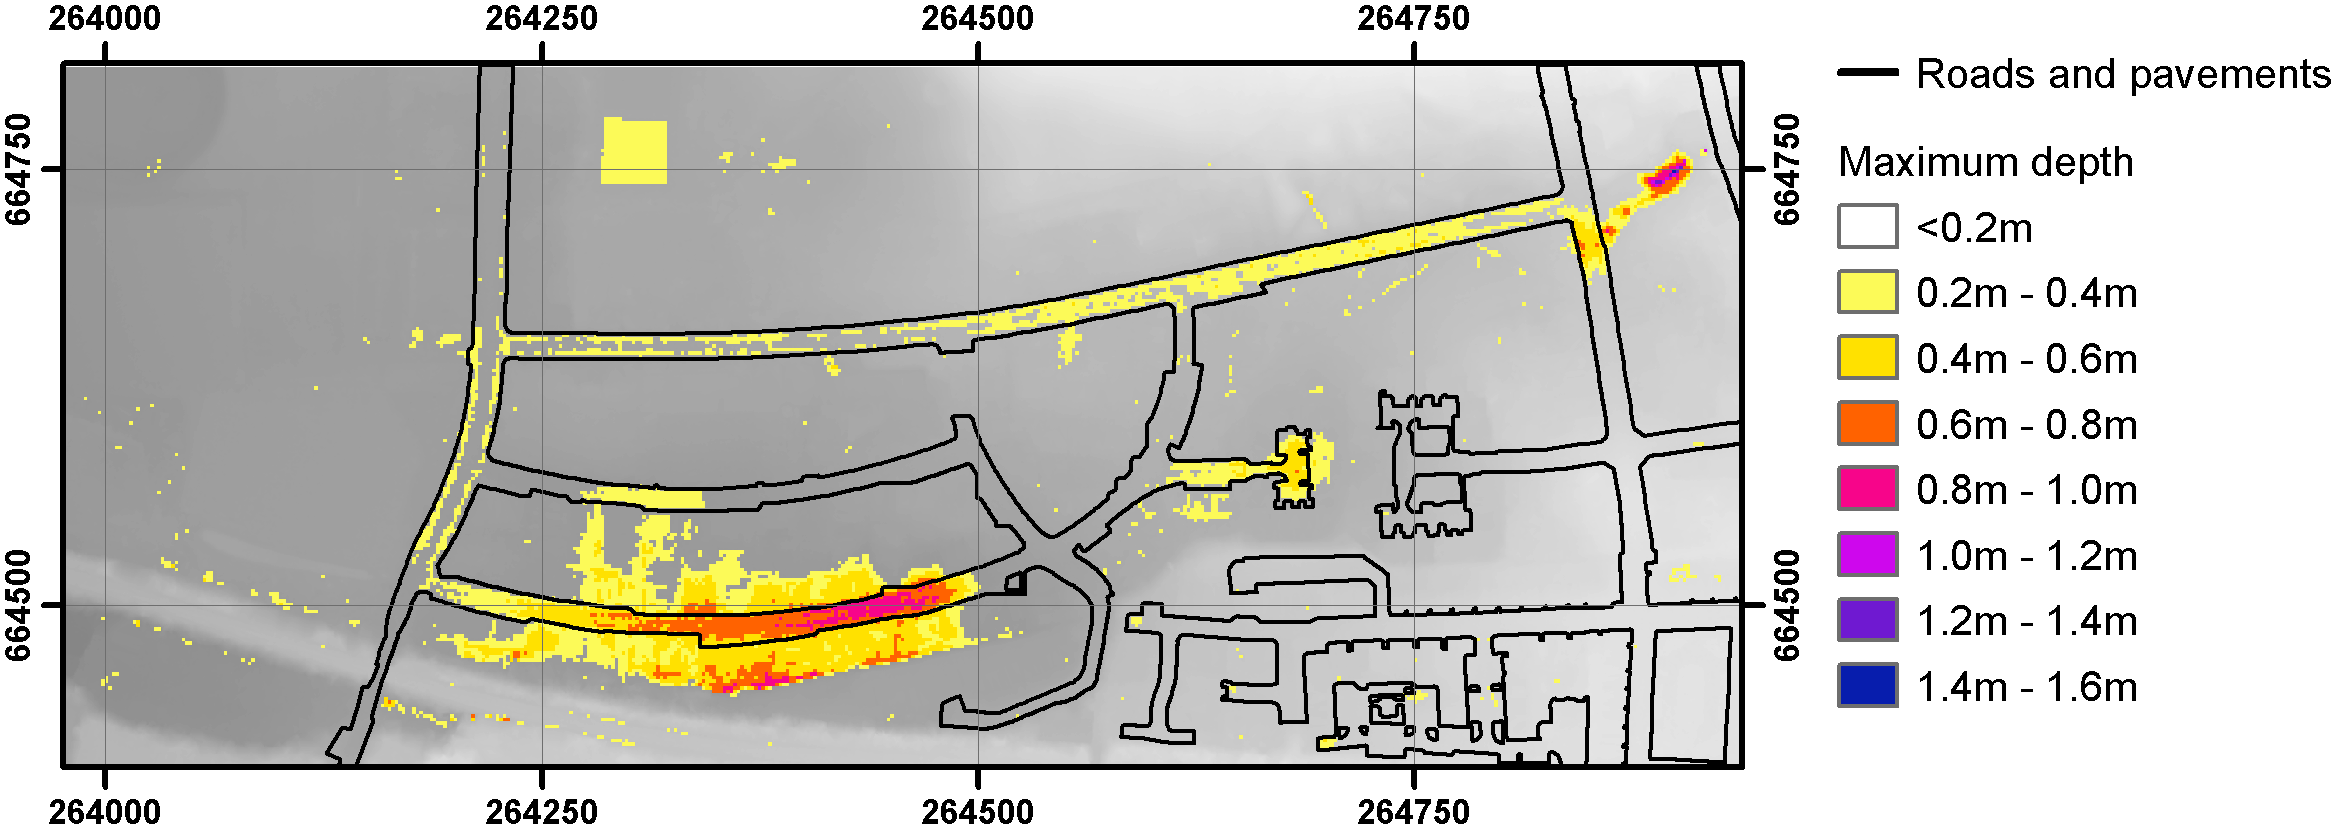
\includegraphics[width=1.0\textwidth]{heterogeneous-dev-figures/Glasgow_MaxDepths.png}
\caption{Maximum water levels observed for the Glasgow test, per cell after 5 hours, shown at 0.2m intervals.}
\label{Glasgow_MaxDepths}
\end{figure*}
\begin{figure*}[tpb]
\centering
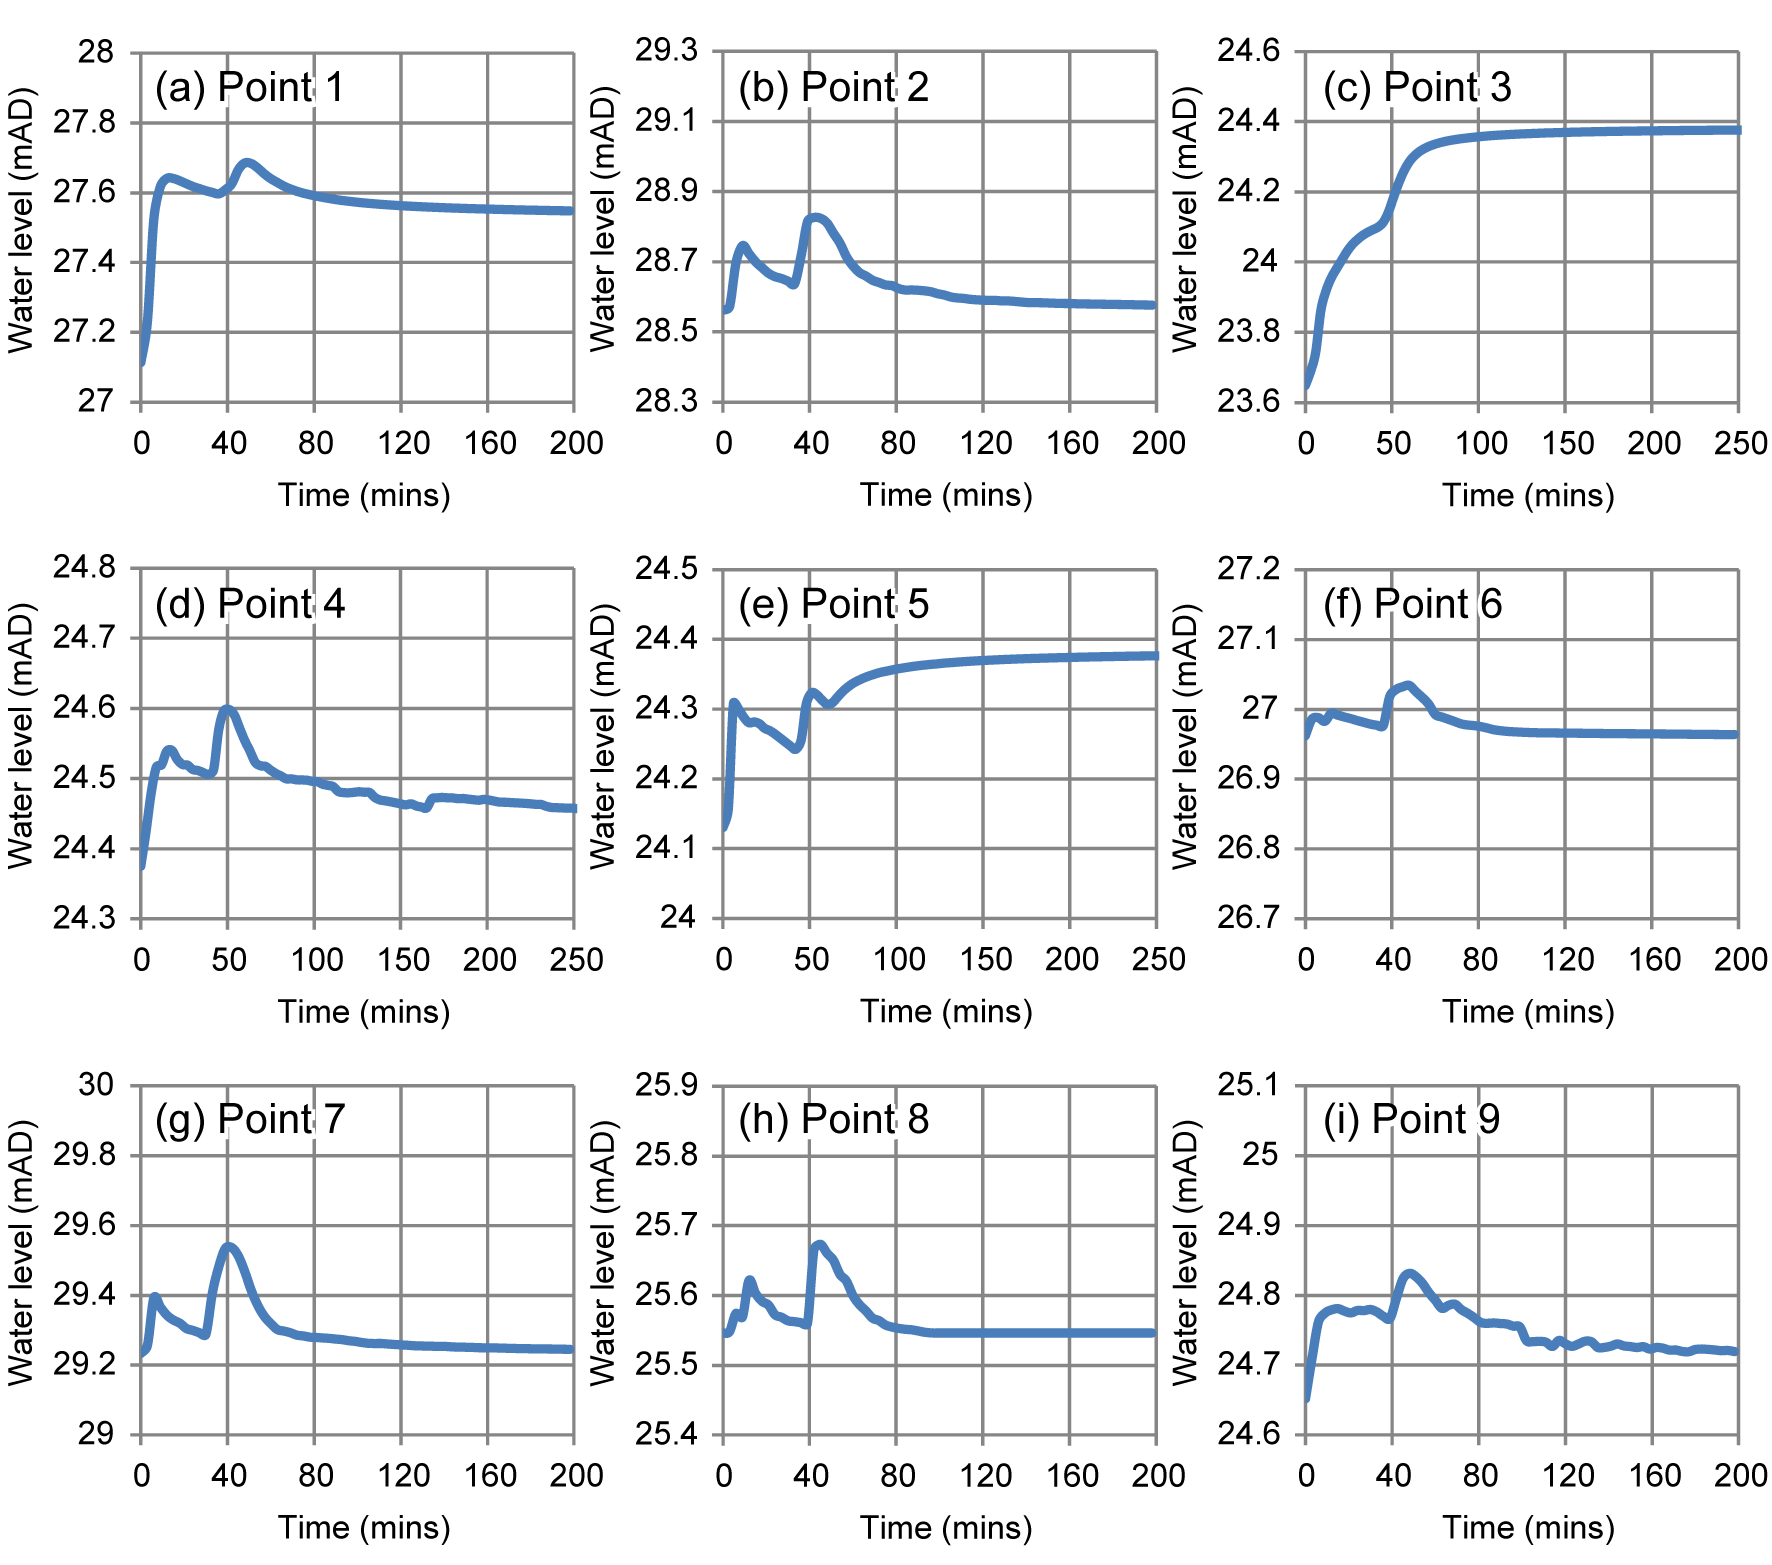
\includegraphics[width=0.8\textwidth]{heterogeneous-dev-figures/Glasgow_PointGraphs.png}
\caption{Changes in recorded water levels for Glasgow, above datum recorded at 9 different sample points in the domain. The location of the sample points is given in Figure \ref{Glasgow_DTM}.}
\label{Glasgow_PointGraphs}
\end{figure*}

The simulation correctly represents the double-peaked nature of the event from intense rainfall and subsequent surcharging of a sewer, with the second peak at point 7 shortly after the surcharging peaked at 38 minutes. The results are generally free of oscillations, except for some small oscillations at point 9 which may be unphysical. At point 2 there is some discrepancy among models as to when the water levels settle after both peaks have passed; the results presented herein suggest this occurs after approximately 120 minutes, which is consistent with the results for the comparable numerical scheme employed in TUFLOW FV. At point 3 the second peak begins at approximately 50 minutes, which is consistent with almost all of the software in \citet{Pender2013}. At point 6 the second peak is predicted to have an elevation around 27.05 mAD, which is higher than many of the other software but there is significant variation across software at this point, ranging from 26.95 to 27.08 mAD. The final flood depths correspond to the areas which were predicted by the majority of software tested in \citet{Pender2013}; clearly a shock-capturing scheme is not necessary to accurately predict the final extent, but can have a marked effect on the progression of the flood wave, localised flow dynamics and arrival timing, all of which could be significant factors in assessing flood risk and crucial in issuing flood warnings. It cannot be asserted as to which software is most accurate as the event and inflow data is hypothetical, however the software herein captures the same behaviour as comparable finite-volume codes solving the full shallow water equations. Small differences in the methods for solving the equations and implementation of boundary conditions can result in significant differences: treatment of wet-dry fronts, frequency of mass addition for precipitation, rounding or smoothing in the consideration of topography, and mechanism for considering the Manning coefficient are believed to be most significant in this instance.

\section{Real-life dam failure at Malpasset (1959)}

The Malpasset dam-break is frequently used as a validation test-case for shock-capturing hydraulic models \citep{Goutal1999}. The double-curvature arch-dam at Malpasset in the south of France failed catastrophically on the 2nd December 1959 at 9:14PM as it approached full capacity during a period of prolonged and intense rainfall. Almost 55,106m\(^{3}\) of water was released downstream towards Fr{\'e}jus, resulting in over 400 deaths. Data is available from a post-event police survey of the extent and a scale model constructed by EDF. The positions of transformers and high-water marks in the valley, plus gauges in the scale model, are indicated in Figure \ref{MalpassetIntro}. A regular Cartesian grid of 10m resolution is used to represent the 18km \(\times\) 10km domain (1.8M cells). The initial free-surface level behind the dam is 100mAD (estimated ±0.5m error), and sea level 0mAD. Comparison of results on the left- and right-hand sides of the valley are presented in Figure \ref{MalpassetValidation} for \(n=0.033\) (\(M=30\)), the value suggested by CADAM project participants.  The first 4000 seconds following the collapse are simulated.

Figure \ref{MalpassetProgression} shows the inundation extent in the valley at \(t=1000\), \(t=2000\), \(t=3000\), and \(t=4000\) seconds. The final extent and agreement with the police survey are consistent with other studies such as \citet{Brodtkorb2011}, with a larger range of parametric sensitivity nearest the dam site. The suggest Manning value is not guaranteed to be transferable between different numerical models and spatial discretisations, but in all instances the police survey falls within the range of parameterisations tested.

\begin{figure*}[tpb]
\centering
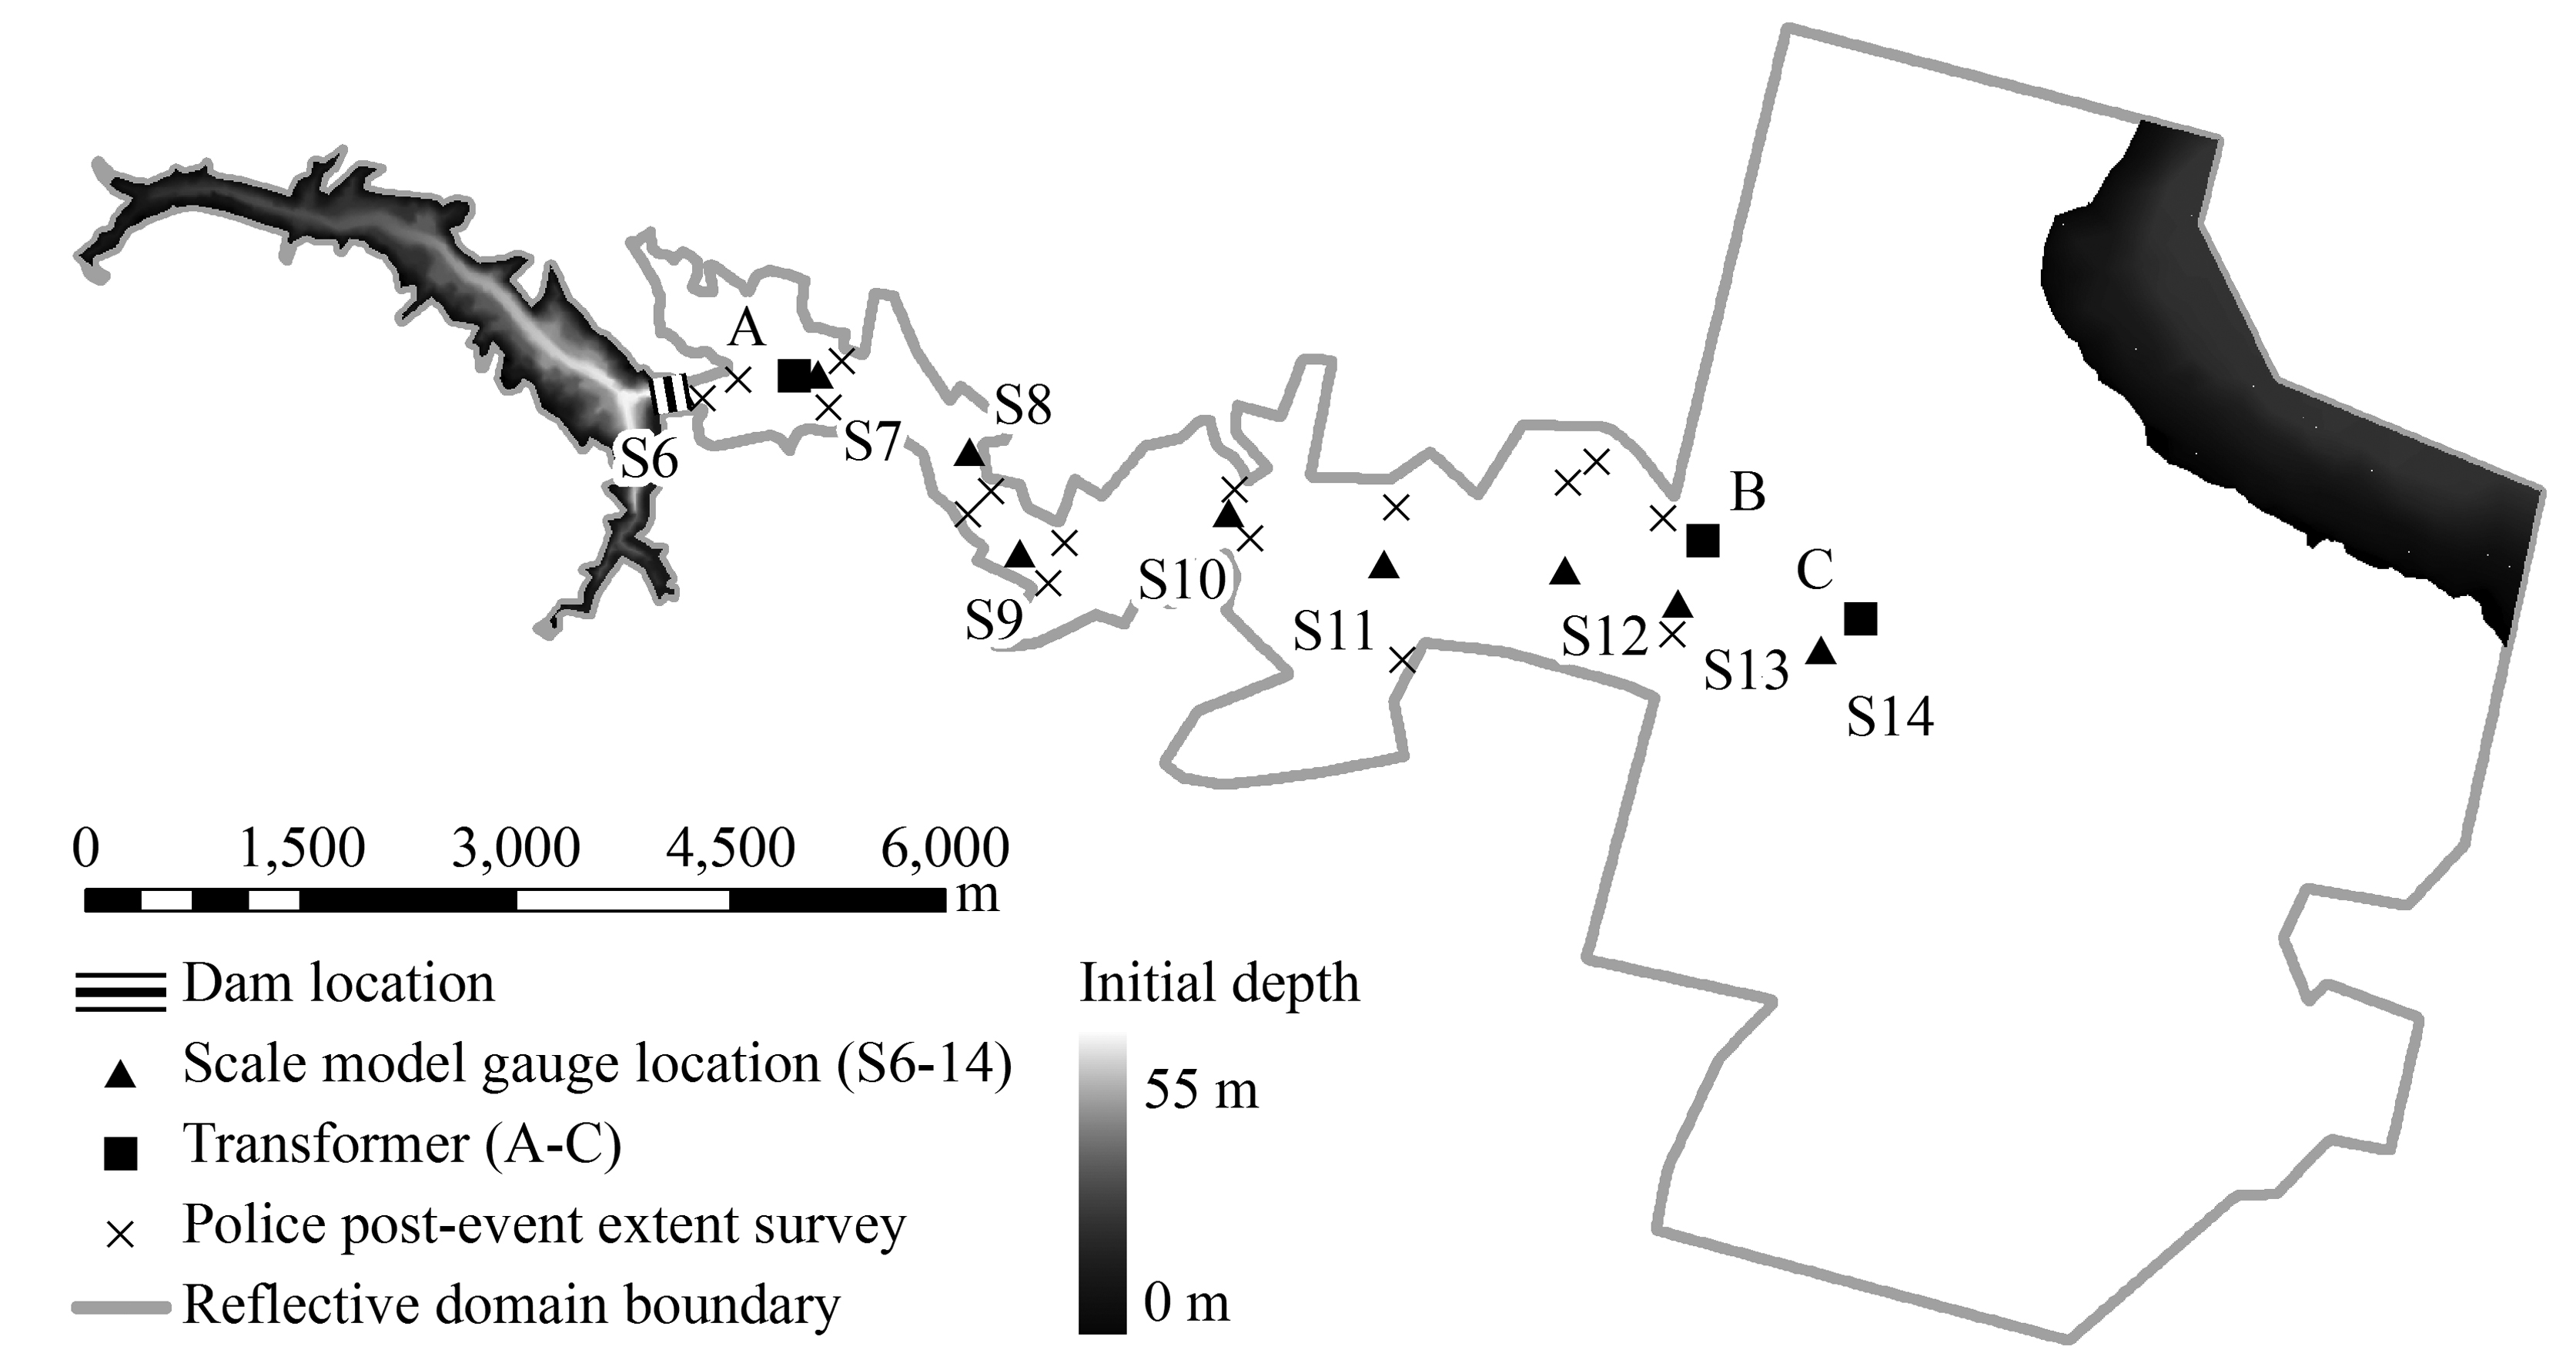
\includegraphics[width=1.0\textwidth]{heterogeneous-dev-figures/Figure_8_Greyscale.jpg}
\caption{Malpasset dam-break domain, initial conditions and locations of validation points.}
\label{MalpassetIntro}
\end{figure*}
\begin{figure*}[tpb]
\centering
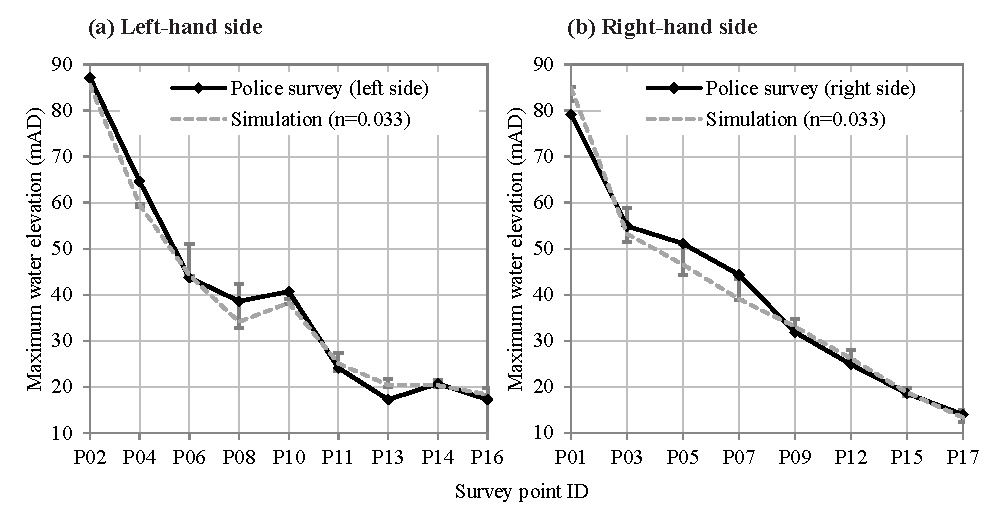
\includegraphics[width=1.0\textwidth]{heterogeneous-dev-figures/Figure_10_Greyscale.pdf}
\caption{Comparison of maximum simulated free-surface levels in Malpasset, on the left- and right-hand sides of the valley (looking downstream) against post-event police survey. Error bars indicate results for $0.022 \le n \le 0.100$ }
\label{MalpassetValidation}
\end{figure*}
\begin{figure*}[tpb]
\centering
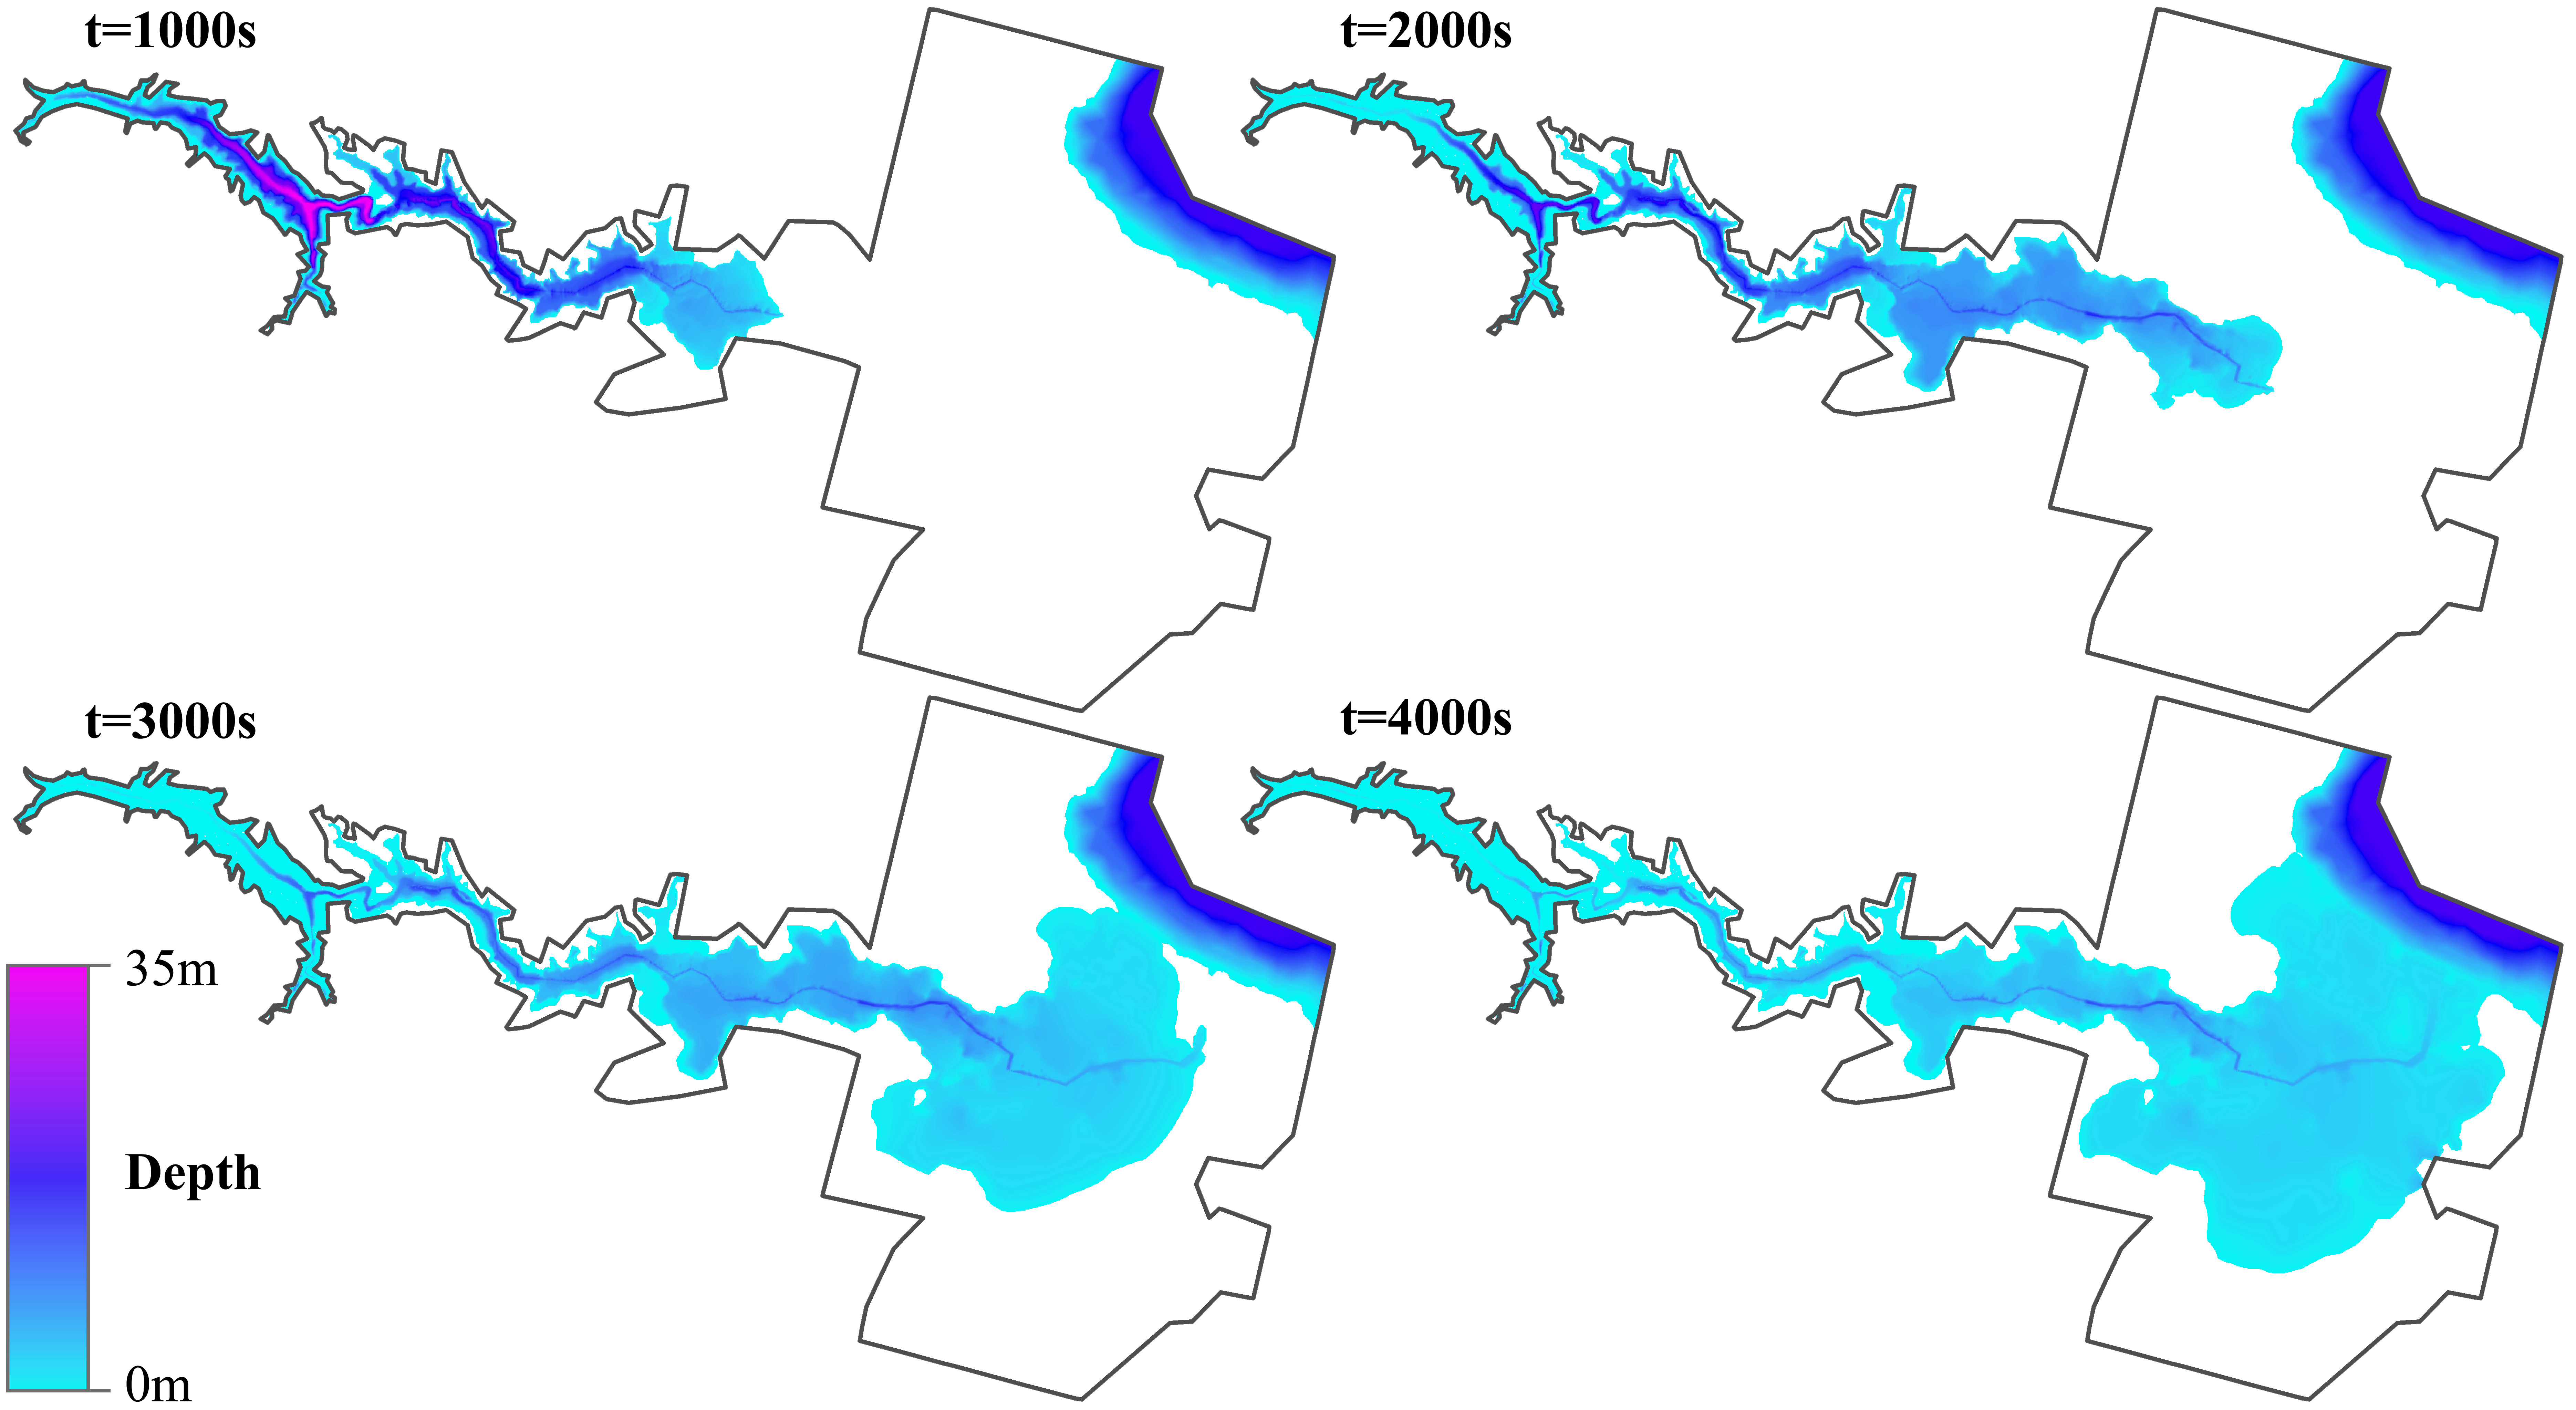
\includegraphics[width=1.0\textwidth]{heterogeneous-dev-figures/Figure_9_Colour.jpg}
\caption{Evolving inundation map for the Malpasset valley every 1000 seconds.}
\label{MalpassetProgression}
\end{figure*}

\section{Computational performance}

The tests at the beginning of this chapter were intended and designed to establish the accuracy of the simulation results, and the suitability for different flow scenarios. The later tests are more suited to performance comparison, as they represent real-world of similar situations. The second-order scheme requires more intensive computation, and it naturally follows that run-times will be longer. Whether the accuracy benefits are justified in the context of longer simulation run-times, is likely to be case dependent and no simple matter. Further performance gains can be achieved by reducing the precision of the calculations, using 32-bit floating-point arithmetic in place of 64 bits. The compound effect of this reduced precision is also discussed here.

\subsection{First-order Godunov-type scheme}

\begin{table*}[pb]
\newcolumntype{R}[1]{>{\RaggedLeft\arraybackslash}p{#1}}
\small
\centering
\caption{Simulation run-times for Glasgow in minutes using three different processing devices.}
\label{GlasgowPerformance}
\begin{tabular}{p{0.15\textwidth}R{0.15\textwidth}R{0.15\textwidth}R{0.15\textwidth}}
\hline
\raggedright{Floating-point arithmetic resolution}	& CPU Intel Xeon E5-2609 & GPU AMD FirePro V7800 		& GPU NVIDIA Tesla M2075 \\
\hline
32-bit 							& 9.05					& 2.47					& 1.98				\\
64-bit 							& 9.45					& 2.67					& 2.88				\\
\hline
\end{tabular}
\end{table*}

The run-times for the Glasgow simulation described earlier in this chapter, using three different processing devices are presented in Table \ref{GlasgowPerformance}. It is important to note however that the domain for this test-case is too small to fully exploit the weak scaling in GPUs. Nonetheless the times represent a significant reduction on those in \citet{Pender2010} and \citet{Hunter2007}, with both CPU and GPU computation, despite the use of an explicit numerical scheme and Godunov-type scheme.

The CPU results are broadly as expected. GPUs however, are designed with 32-bit computation as their primary purpose. The AMD GPU should exhibit inferior performance to the NVIDIA Tesla, according to the device specifications. The disparity can likely be attributed to the overheads, and not providing a suitably large domain to fully leverage these devices.

Compared to figures reported for the same test in \citet{Pender2013}, the software presented herein is slightly slower than some comparable GPU software (e.g. 1.40 minutes for TUFLOW GPU), which may in part be a result of using OpenCL parallelisation, where there is some evidence to suggest memory transfers and dispatch overheads could be slightly higher than CUDA \citep[e.g.][]{Karimi2010}. The performance results cannot be directly compared however as different hardware was used for each software. Moreover, the CUDA and OpenCL APIs have subtle but important differences between implementations, such as the non-standard blocking behaviour of \texttt{clEnqueueNDRangeKernel} in NVIDIA's implementation of OpenCL, where a call scheduling work on the GPU will not return until the work is complete, making it impossible to queue many iterations of the numerical scheme to reduce the launch overhead. Comparison is also difficult as diffusion approximation codes \citep[e.g.][]{Bates2000} can be expected to exhibit poor computational efficiency at 2m resolution because of a more severe timestep constraint.

\subsection{Second-order MUSCL-Hancock scheme}

\begin{table*}[tb]
	\small
	\centering
	\caption{Total simulation time and cell calculation rate using three different devices, cache configurations and floating-point precisions, for the Malpasset dam failure second-order simulation. The kernel and cache configurations are described in Chapter \ref{chapter:NumericalMethods} and Figure \ref{Kernels}.}
	\label{Malpasset_PerformanceResults}
	\begin{tabular}{llrrrrrr}
		\hline
		& 			& \multicolumn{2}{c}{AMD FirePro V7800}			& \multicolumn{2}{c}{NVIDIA Tesla M2075}			& \multicolumn{2}{c}{Intel Xeon E5-2609} 	\\
		Kernels/cache 		& Precision 	& \begin{tabular}[t]{@{}c@{}}Time \\ (s)\end{tabular} 	& \begin{tabular}[t]{@{}c@{}}Rate \\ (x10\textsuperscript{6}/s)\end{tabular} 	& \begin{tabular}[t]{@{}c@{}}Time \\ (s)\end{tabular} 	& \begin{tabular}[t]{@{}c@{}}Rate \\ (x10\textsuperscript{6}/s)\end{tabular}	& \begin{tabular}[t]{@{}c@{}}Time \\ (s)\end{tabular} 	& \begin{tabular}[t]{@{}c@{}}Rate \\ (x10\textsuperscript{6}/s)\end{tabular} 	\\
		\hline
		A: None 				& 32-bit 		& 84 			& 435	 		& 66 			& 556	 		& 821 		& 45	 \\
		& 64-bit 		& 363 		& 106	 		& 243 		& 159	 		& 1534 		& 25	 \\
		B: Normal				& 32-bit 		& 142 		& 258	 		& 125 		& 294	 		& 956 		& 38	 \\
		& 64-bit 		& 446 		& 86		 		& 381 		& 101	 		& 1730 		& 22	 \\
		B: Oversized			& 32-bit 		& 122 		& 300	 		& 88 			& 417	 		& 951 		& 39	 \\
		& 64-bit 		& 442 		& 87		 		& 366 		& 105	 		& 1739 		& 22	 \\
		C: Normal				& 32-bit 		& 122 		& 298	 		& 117 		& 314	 		& 1136 		& 32	 \\
		& 64-bit 		& 844 		& 45		 		& 576 		& 67		 		& 2818 		& 14	 \\
		C: Oversized			& 32-bit 		& 110 		& 335	 		& 88 			& 417	 		& 1144 		& 32	 \\
		& 64-bit 		& 820 		& 47		 		& 554 		& 69		 		& 2881 		& 13	 \\
		\hline
	\end{tabular}
\end{table*}

The run-times with multiple configurations of the software developed herein are presented in Table \ref{Malpasset_PerformanceResults} for the different hardware used to simulate the Malpasset event. The results indicate that for 64-bit computation the NVIDIA GPU model can simulate the Malpasset collapse 6.3$\times$ faster than the Intel CPU, while the manufacturer-quoted peak performances suggest a 6.7$\times$ difference \citep{NVIDIACorporation2011,IntelCorporation2012}; the actual and and quoted performance differences for the AMD device are 4.2 and 5.2 respectively \citep{AMD2012}. This is not altogether surprising; further analysis suggests the AMD device with 64-bit floating-point does not achieve full occupancy because the number of registers constrains the number of AMD wavefronts. Nonetheless the AMD simulation time represents a significant improvement over the CPU, for a fraction of the cost of an NVIDIA Tesla GPU (per Table \ref{CPUGPUCosts}). Vendor-quoted peak performance levels are rarely achievable in practical applications and are compared only to give an indication of device processing power. For users without a suitable GPU the software will nevertheless provide a significant performance boost, given that the new software fully harnesses all four cores of the CPU at all stages of the numerical scheme, unlike most existing commercial software.

Caching data to local memory provides no performance benefit with 32- or 64-bit floating-point computation for any of the devices tested herein. Where local memory is used however, oversizing the array is often shown to improve performance by alleviating bank conflicts, for the reasons previously outlined in Section \ref{Subsection:StorageMemoryHeterogeneous}.

\section{Effects of floating-point precision}

\begin{figure*}[p]
	\centering
	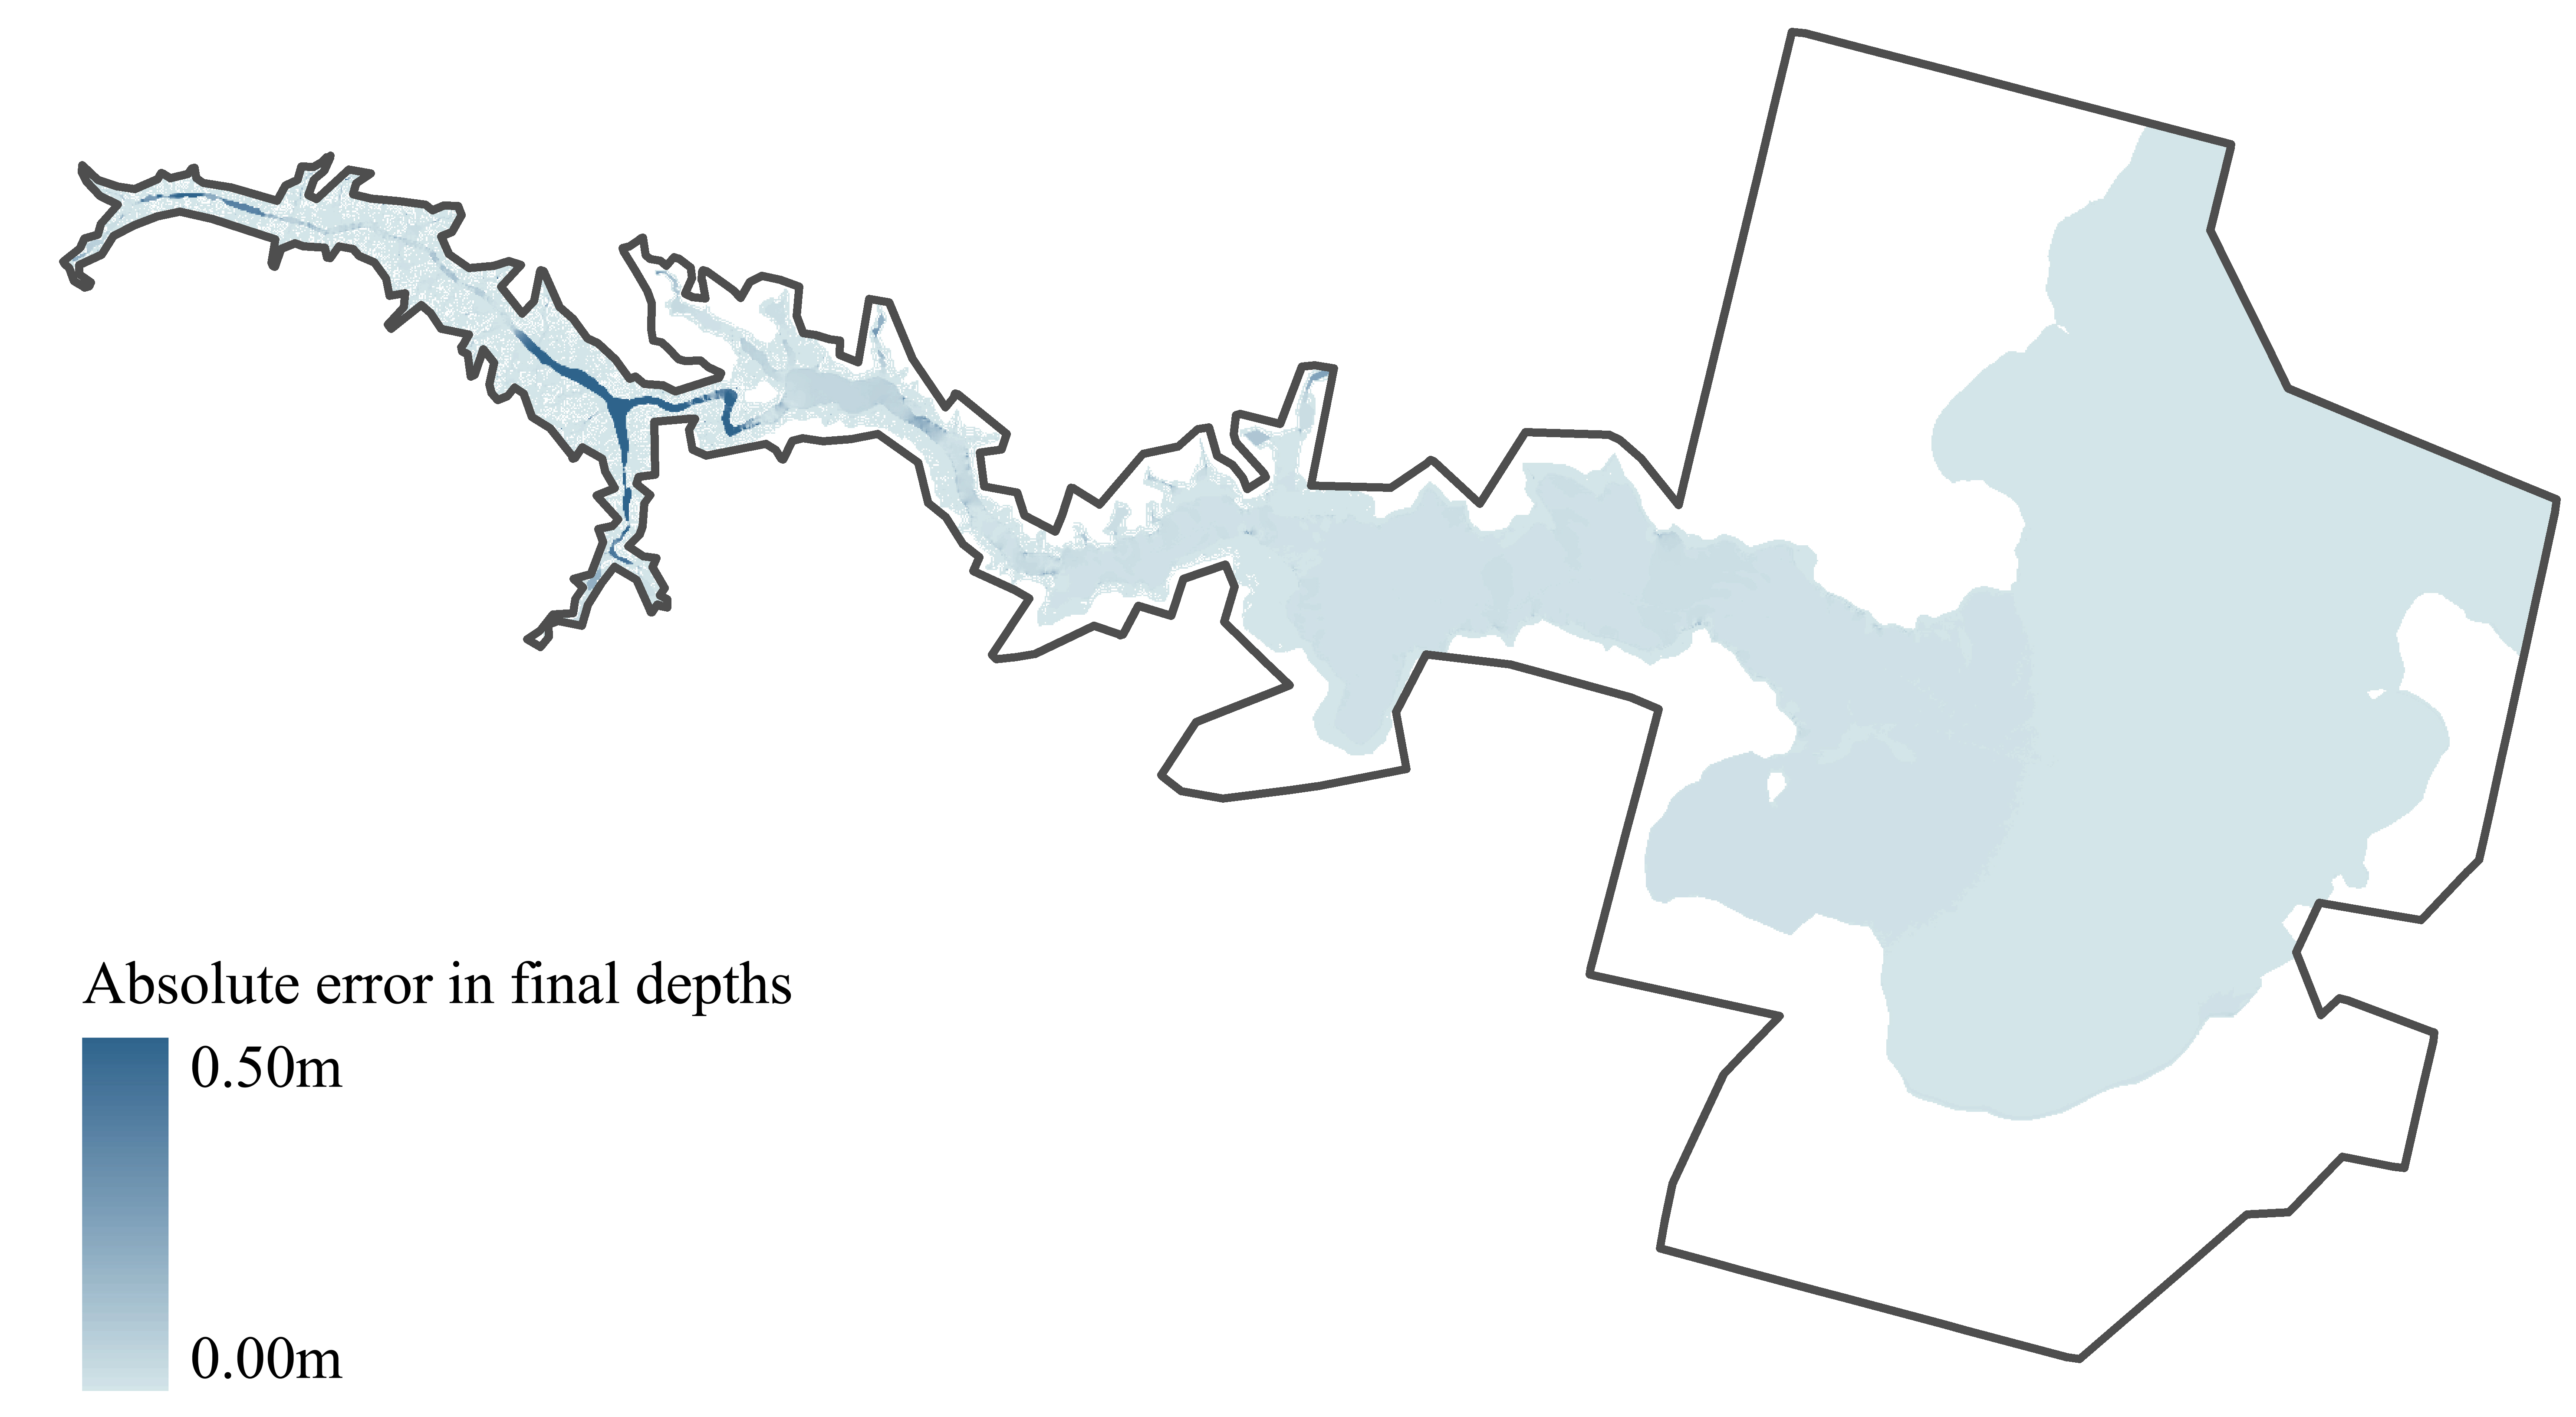
\includegraphics[width=1.0\textwidth]{heterogeneous-dev-figures/Figure_11_Colour.jpg}
	\caption{Spatial distribution of absolute errors in Malpasset, introduced in the final depths (4000s) by using 32-bit floating-point after the Malpasset collapse, when compared to 64-bit results.}
	\label{FPErrorFinal}
\end{figure*}
\begin{figure*}[p]
	\centering
	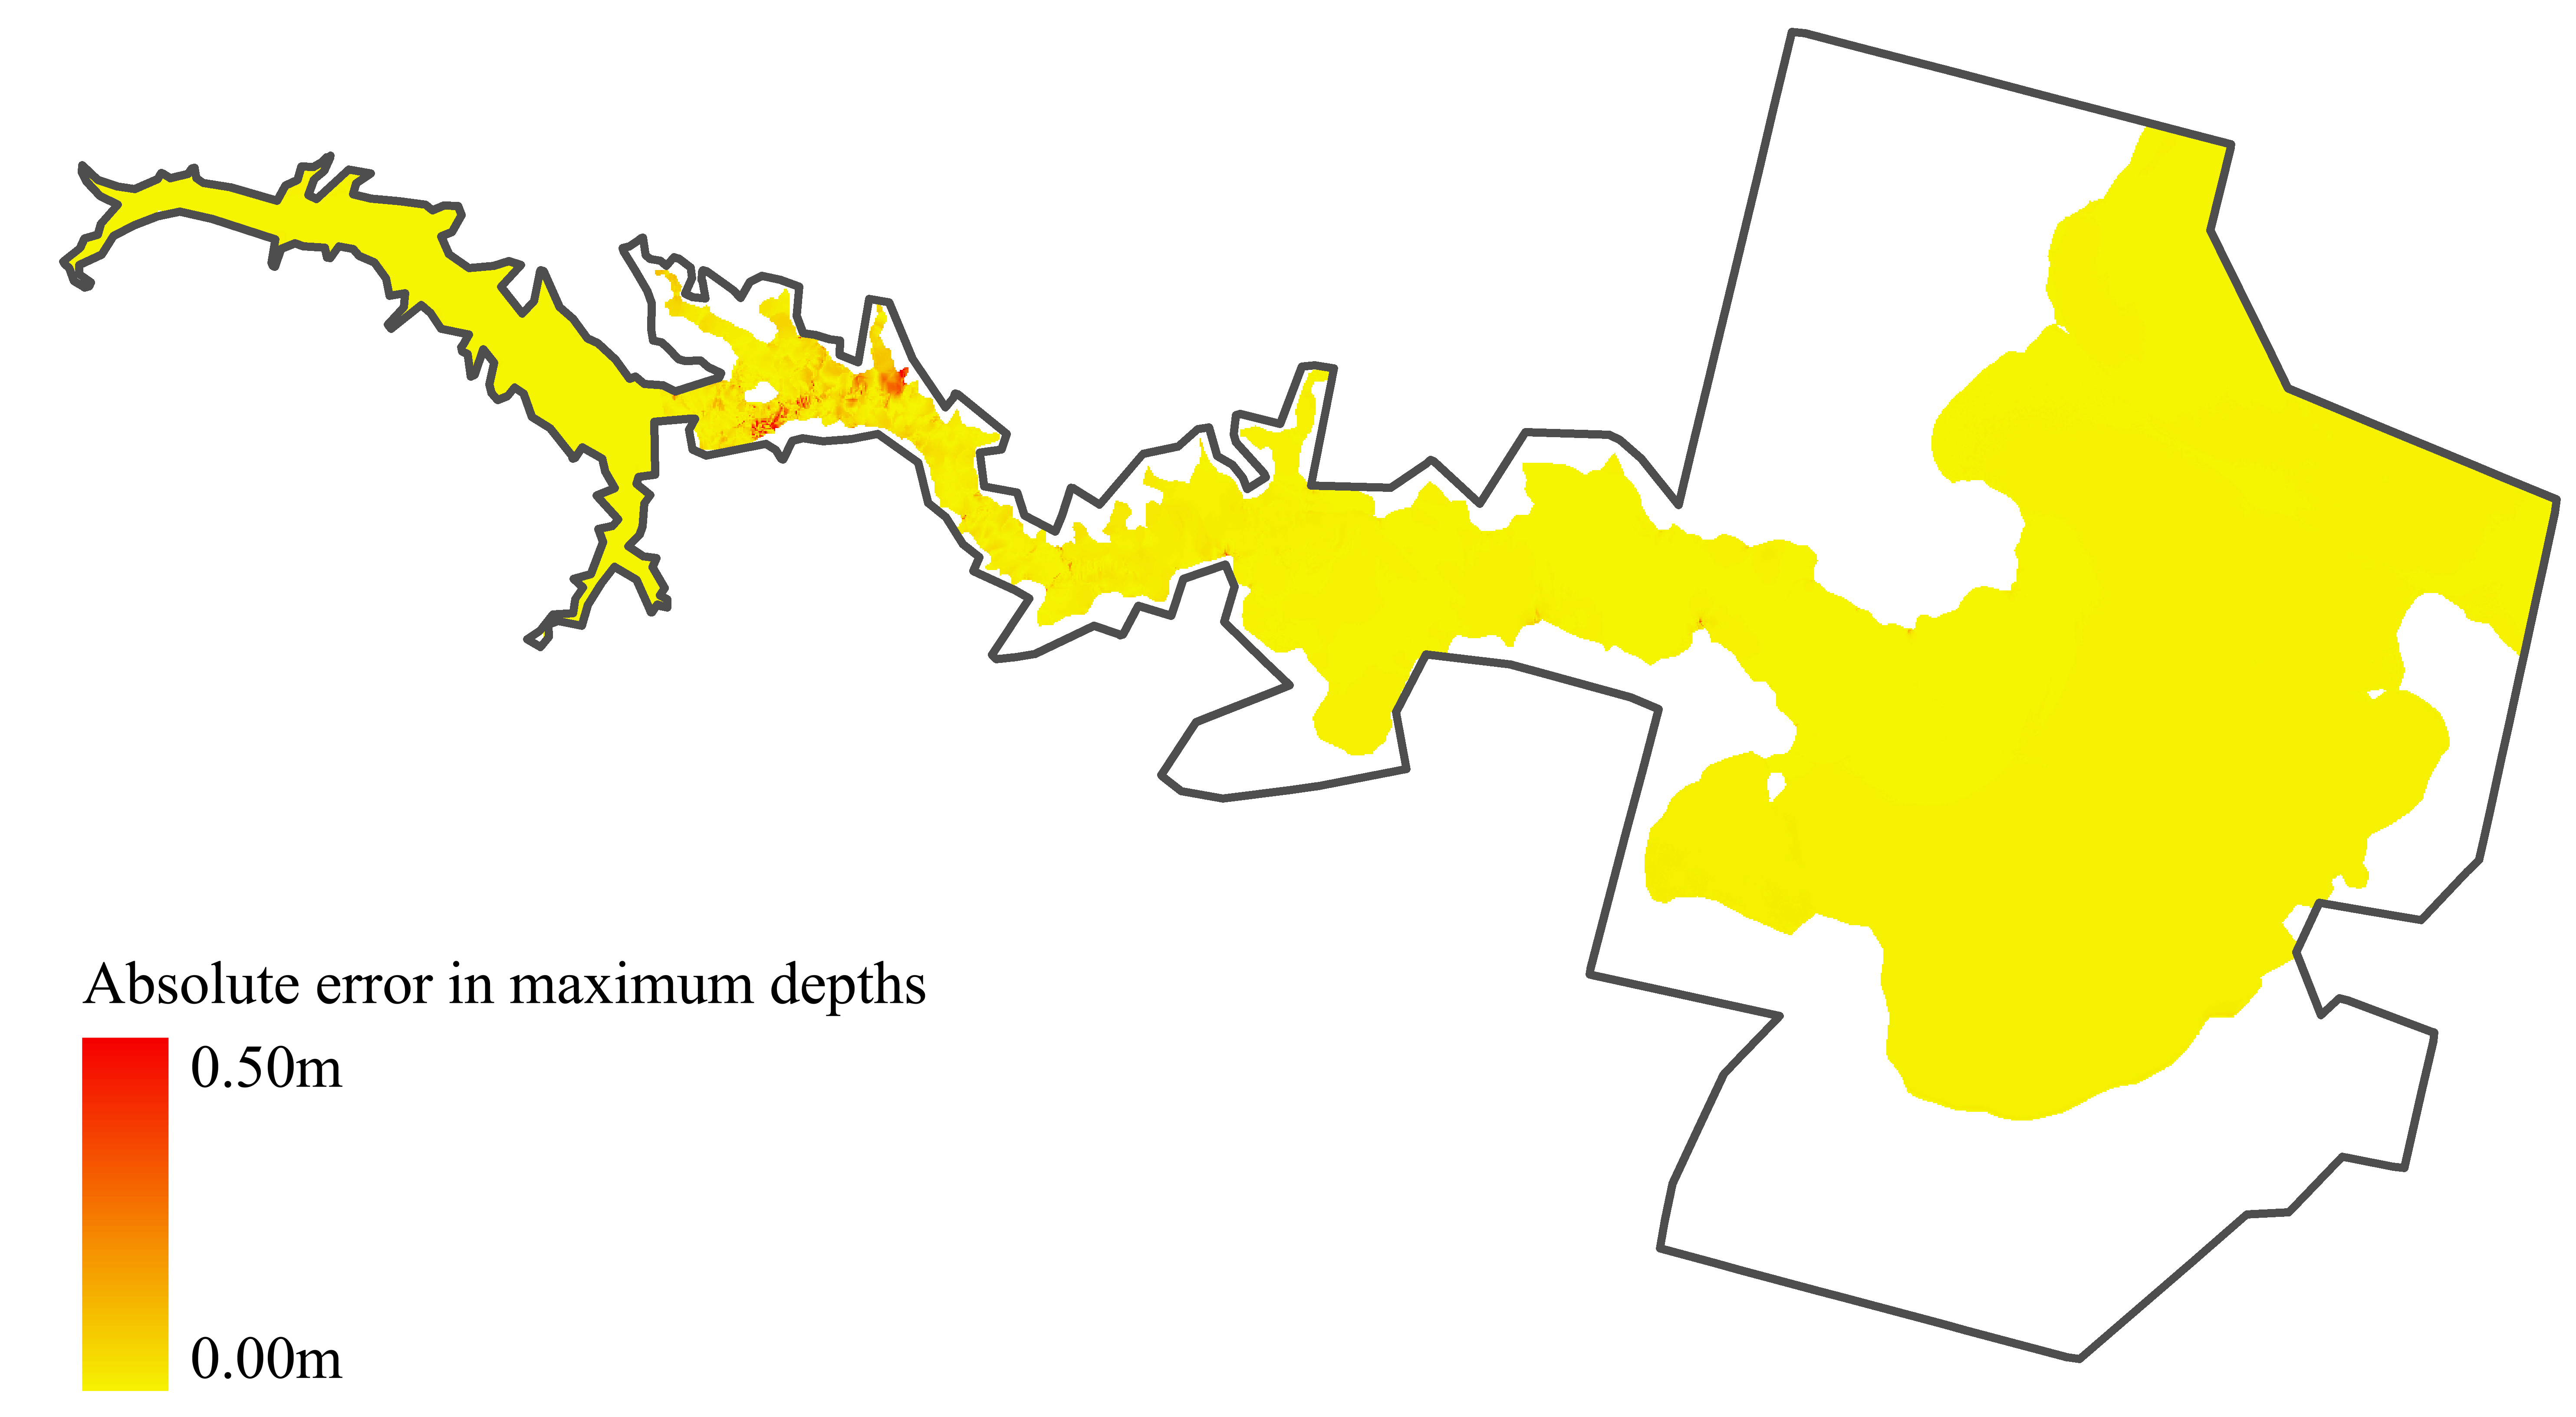
\includegraphics[width=1.0\textwidth]{heterogeneous-dev-figures/Figure_12_Colour.jpg}
	\caption{Spatial distribution of absolute errors in Malpasset, introduced in the maximum depths by using 32-bit floating-point after the Malpasset collapse, when compared to 64-bit results.}
	\label{FPErrorMax}
\end{figure*}

In all simulations carried out 32-bit computation was faster than 64-bit. There are substantial and significant differences in the results obtained however, which demonstrate that 32-bit introduces unacceptably large errors. The spatial distribution of errors in the final and maximum simulated depths are shown in Figure \ref{FPErrorFinal} and Figure \ref{FPErrorMax} respectively.  Errors in maximum depth are concentrated in areas with the greatest flow velocities and where shocks are observed immediately downstream of the dam, whereas the final depth errors mainly lie in the shoal zones of the catchment where water should drain. While the mean error in final depths with 32-bit is \(<0.05\)m, the greatest error was \(+1.89\)m, and for the maximum depths the greatest error was \(+0.85\)m. The technique adopted herein uses free-surface level as a conserved variable instead of depth, which reduces the numerical resolution of shallow depths in particular. Whilst the localised errors may be a by-product of the specific numerical scheme employed herein, the author urges caution and encourages further research before 64-bit precision is dispensed with for performance over accuracy.

Other authors have previously reported the differences between 32- and 64-bit floating-point in terms of a mass balance error introduced by successive rounding \citep[e.g.][]{Brodtkorb2010a}, which potentially overlooks the significant magnitude of localised errors. Unlike this study they conclude that 32-bit floating-point provides an acceptable degree of accuracy. This difference stems from the different numerical scheme employed herein. Mixing different levels of precision remains a possibility. 

\section{Conclusions}

In this chapter, the numerical and computational performance of the software was tested using different processing devices and levels of floating-point precision. The numerical performance appears consistent with other software and published results, whilst the numerical scheme employed is shown to influence results significantly in some cases, suggesting second-order accuracy is important especially in dam-break scenarios or those with frequently-changing wet-and-dry fronts. 

In respect of the tests considered in this chapter, it can be determined that:

\begin{itemize}
	\item the numerical schemes employed are both capable of representing the well-balanced property, exhibiting a static condition over a complex and varying bed topography, without problem;
	\item there are limitations to the applicability of the first-order solution, when dealing with continually changing wet-dry fronts over a long time period with a high grid resolution, and thus for tidal applications (which have much in common with the dam-break over an emerging bed), a second-order solution may be required, whilst for most progressive flood cases (fluvial and pluvial) the zone of inundation generally only expands;
	\item even when a second-order solution is employed, the speed of the wave front may be underestimated for dam break situations, caused by a combination of the limitations and assumptions of the shallow water equations, and the numerical scheme's approach to maintaining stability;
	\item with adequate spatial discretisation, complex phenomena such as the interaction between shock and rarefaction waves can be simulated correctly, as evidenced by the dam-break against a fixed obstacle, but accepting there are nonetheless discrepancies when compared against laboratory measurements;
	\item flows of a very shallow depth can be correctly simulated, such as in the case of intense rainfall during the Glasgow benchmark case, where the results are consistent with commercial software;
	\item use of single-precision (32-bit) arithmetic introduced considerable errors in the mass conservation for Glasgow, and depths at a critical point for Malpasset, and hence cannot be recommended for general use, without thorough sensitivity testing;
	\item performance tuning parameters and options, such as caching interim values during a second-order simulation, and alignment of variables in memory, made very little difference to the overall computational performance in many cases;
	\item satisfactory results were achieved for tests in which flooding was caused by pluvial, dam failure, and defence failure mechanisms;
	\item the processing device used made no discernible difference in the results (typically fractions of a millimetre in depth); and
	\item whether the additional computational overhead associated with the second-order solution is worthwhile in real-world cases requires professional judgement, with respect to the other uncertainty inherent in topographic and observational data.
\end{itemize}

Clear performance benefits are evident from GPU computation when compared to multi-core CPU use, however most of the the simulations presented herein have not been sufficiently large to fully capitalise on the GPU benefits. Later chapters include simulations for entire cities, and present an opportunity to further explore the performance benefits in practical applications.

\chapter{Application to fluvial flooding and analysis of the impacts of grid resolution and parameterisation}
\label{chapter:Fluvial}

The previous chapter considered a wide range of cases to evaluate the software's numerical and computational performance. It is necessary to simulate flooding at the scale of entire cities, to reproduce recent events such as the flooding in Carlisle (2005), New Orleans (2005), Hull (2007), Morpeth (2008), Leeds (2015), and Whitby (2016). Simulation of these complex urban environments requires advances in software, as described previously, to deliver results in a timely manner. This becomes even more pertinent for applications in real-time flood simulation, for incident management and forecasting. In doing so, new problems are also presented, such as the transferability of parameterisations between different grid resolutions, and the resolution beyond which diminishing returns are expected.

This chapter considers these practical matters of parameterisation and transferability, starting by applying the high-performance computing methods to simulate a real-world fluvial flood event, caused by defence overtopping, and comparing the results with a range of grid resolutions and parameters, to one of the most comprehensive post-event survey datasets available. A defence failure event is then considered, which in the absence of a suitable real-world dataset, is simulated as a hypothetical event near London used elsewhere in literature, with relative comparisons.

\section{Flooding in Carlisle, January 2005}

The new software has been applied to simulate flooding in Carlisle, North West England, in January 2005. Over 200mm of rain fell in a few hours over the Cumbrian mountains, believed to be equivalent to a \(1\%\) annual exceedance probability (AEP) event. Rivers quickly responded, with a volumetric discharge exceeding 1,500 m\textsuperscript{3}s\textsuperscript{-1} recorded within Carlisle itself on the River Eden, downstream of its major tributaries, the Rivers Petteril and Caldew. Severe flooding ensued, in an event that played out over more than 48 hours, affecting over 6,000 residents and directly flooding over 1,900 properties \citep{GONW2005,EnvironmentAgency2006a}.

In the week that followed both the Environment Agency (EA) and Bristol University conducted differential global positioning system (DGPS) surveys of water and wrack marks, their combined efforts creating one of the most comprehensive validation datasets for modelling urban flood inundation with 263 individual points. Different software codes and modelling techniques have since been applied to reproduce the event, most notably \citet{Neal2009}, \citet{Horritt2010}, \citet{Fewtrell2011a} and \citet{Liu2013}.

\begin{figure*}[tpb]
\centering
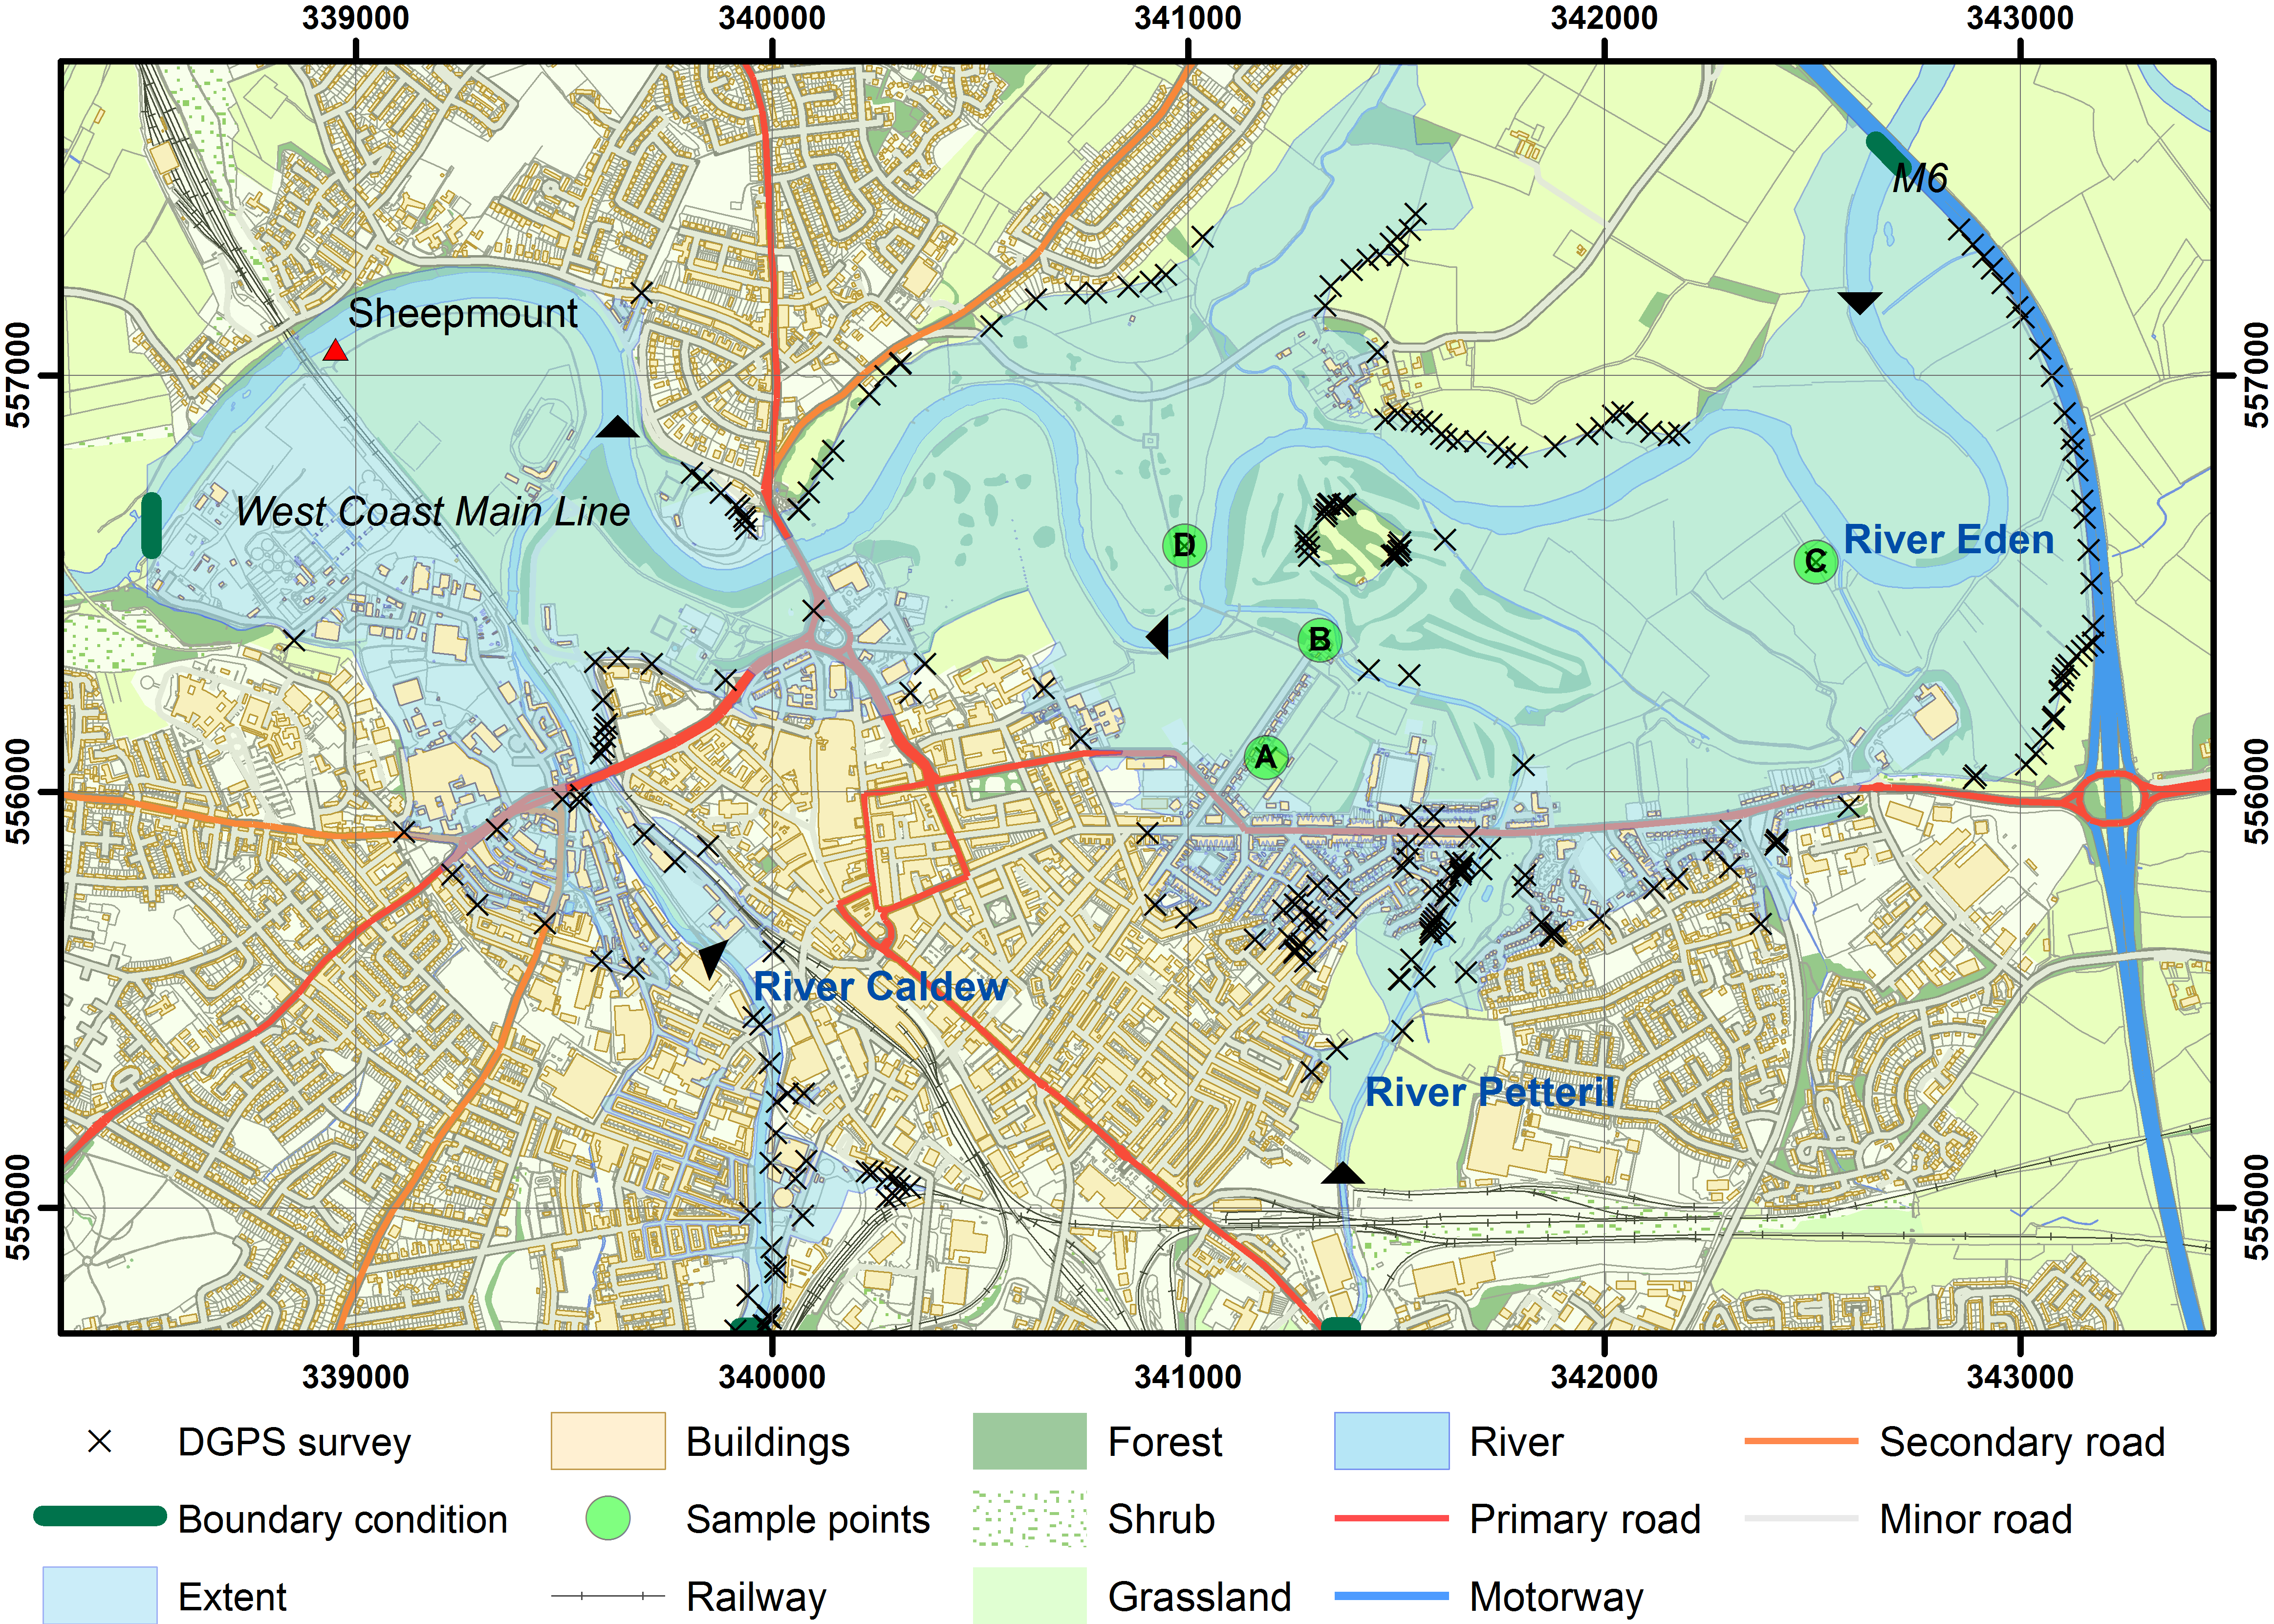
\includegraphics[width=1.0\textwidth]{carlisle-figures/Figure3.png}
\caption{Extent and topographic features for Carlisle with the three rivers and flow directions indicated.}
\floatfoot{Topographic data used in figure is \copyright{} Crown Copyright/database right 2013. An Ordnance Survey/EDINA supplied service.}
\label{CarlisleMap}
\end{figure*}
\begin{figure*}[tpb]
\centering
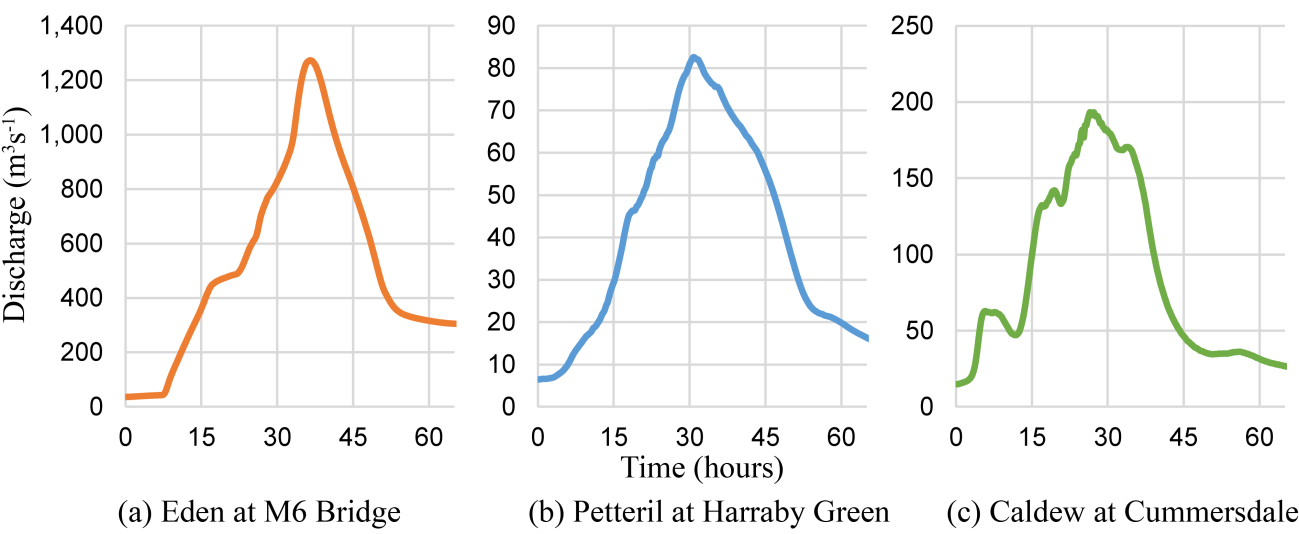
\includegraphics[width=0.9\textwidth]{carlisle-figures/Figure4.png}
\caption{Volumetric discharge inflow for the three rivers during the event.}
\label{BoundaryDischarges}
\end{figure*}

The topographic features, three rivers concerned, location of validation points, and approximate extent of the flood are shown in Figure \ref{CarlisleMap}. The root mean square error (RMSE) of the DGPS measurements is believed to be approximately 0.5m. The extent is deduced from a combination of EA records and the survey points, hence has buildings removed to create an appropriate mask for use with a high-resolution digital elevation model (DEM); for clarity this is different to the extent used by \citet{Horritt2010}. Inflow hydrographs for the three rivers are shown in Figure \ref{BoundaryDischarges}. The effects of rainfall within the city are neglected herein, to allow comparison with other published studies reproducing the event, and also because data is lacking for the sewer network and there is only anecdotal evidence detailing the sewer surcharging. 

\subsection{Model generation}

Fluvial flooding, in which defences are over-topped typically results in both slow velocities and a gradual evolution of the flood extent, except in cases where the defences are substantially overwhelmed, or fail completely. The nature of a gradual flood inundation event is such that minimal shocks would be expected, thus a first-order solution is considered to be an appropriate choice.

The topography for the model is produced from 2m DTM data provided by the Environment Agency Geomatics Group (EAGG). This product represents the lowest return value from the altimetric LiDAR surveys conducted, with interpolation (typically on a TIN basis) used to address any gaps. This generally provides a high quality representation of the ground level except in densely forested areas, in the author's experience. The highest return values represent the DEM product (referred to as DSM by EAGG), and include buildings but also street furniture, trees and shrubs. These latter items all create a partial barrier to flow, but not an absolute barrier. To ensure only buildings are included from the DEM, an extract is clipped using building outlines from Ordnance Survey's MasterMap product, and superimposed on the DTM data. No consideration is given herein to the partial obstructions created by street furniture, trees and shrubs, but it is recognised that some authors use sub-grid parameterisation or increase the roughness coefficient to address this \citep[e.g.][]{Bates2003,Yu2006,Casas2010,Chen2012}.

The LiDAR data obtained by EAGG cannot penetrate water to a substantial depth, thus is inadequate for representing the main channel of rivers. Data from a cross-sectional survey was interpolated along a spline of the river centreline to create a gradually-transitioning representation of the river bed, referenced against the same datum as the LiDAR data. This was superimposed atop the aforementioned DEM/DTM blend data, thereby excluding buildings which cantilever over the river, and with bridge supports manually added back to the data afterwards, perchance they should create a noteworthy flow constriction and backwater effect.

Once calibrated, simulations were executed with three different processing devices from each of the mainstream vendors to compare run-times. CPU simulations at high resolutions even using all four cores of the Intel Xeon E5-2609 would have taken several days to complete, hence were not run to completion. The vendor-quoted computational power of the two devices is 77 GFLOPS for the Intel Xeon E5-2609 \citep{IntelCorporation2012}, and 515 for the NVIDIA Tesla M2075 \citep{NVIDIACorporation2011}, representing a theoretical improvement of 6.7 times for the scientific GPU. The calibration procedure is described in the next section.

\subsection{Effect of grid resolution and parameterisation}

\begin{figure*}[tpb]
	\centering
	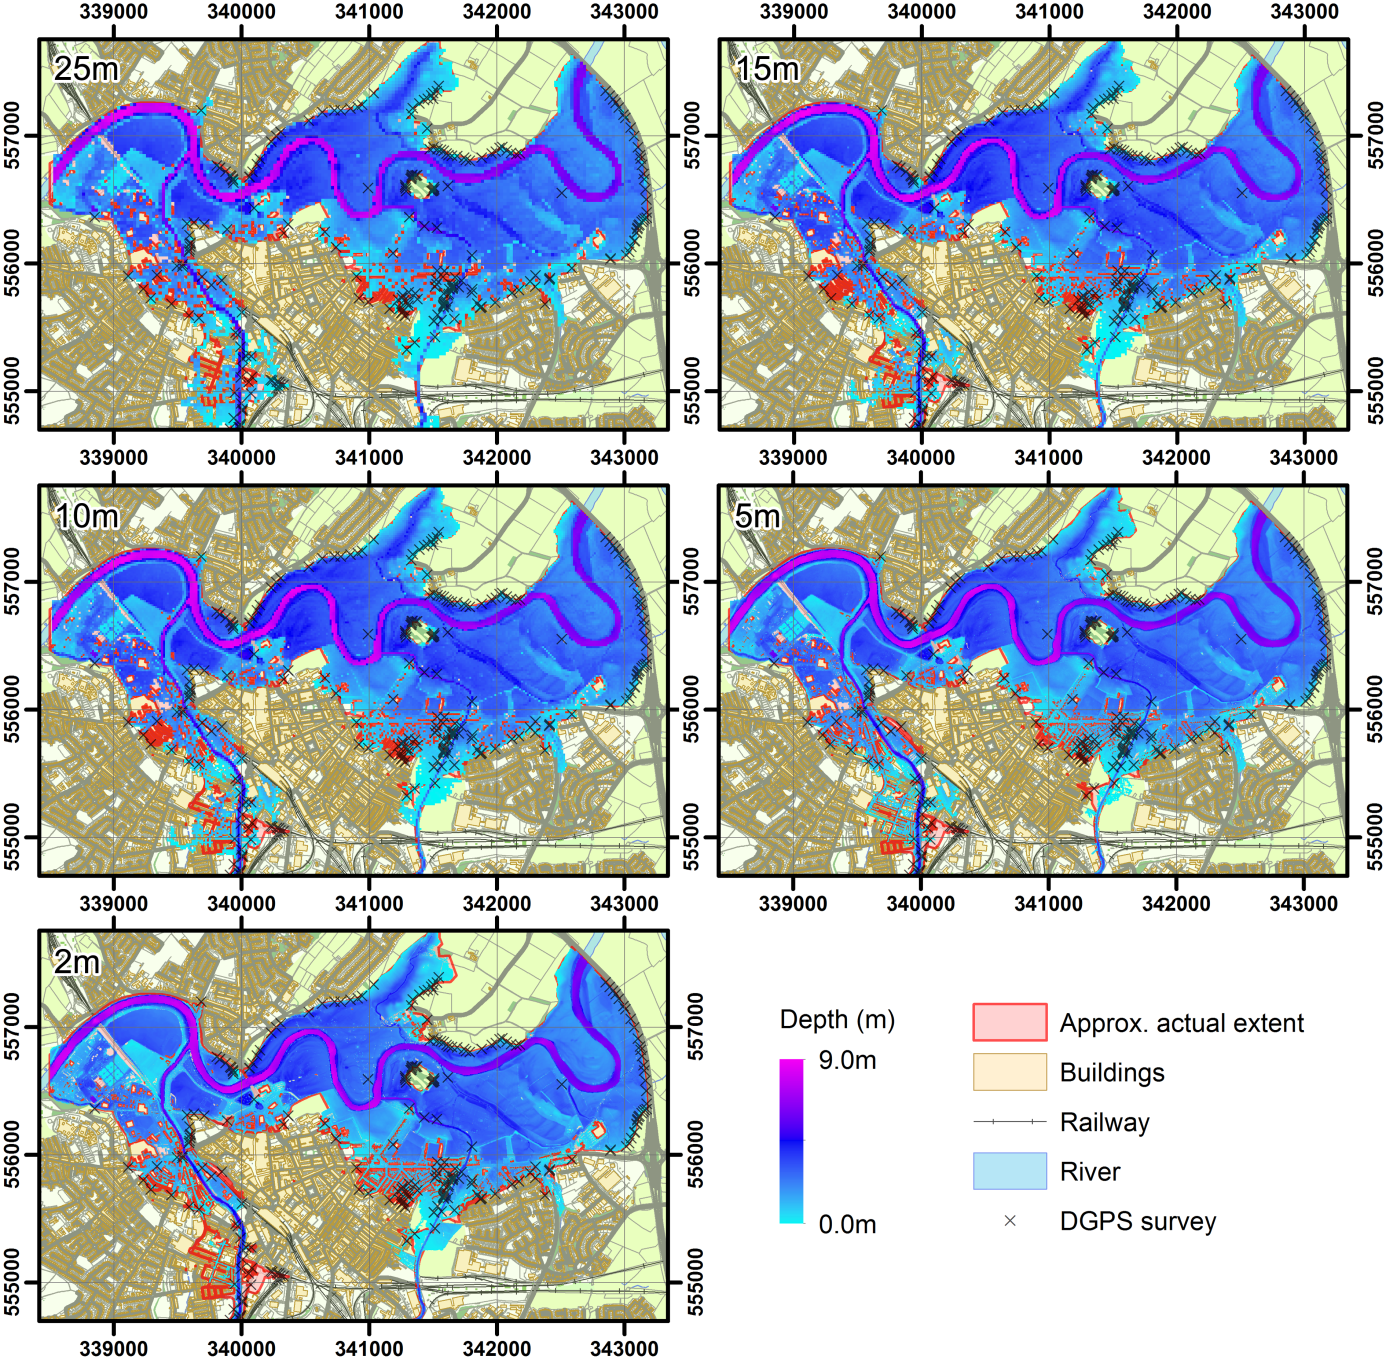
\includegraphics[width=1.0\textwidth]{carlisle-figures/Figure5.png}
	\caption{Maximum depths for calibrated simulations at different spatial resolutions.}
	\label{MaxDepths}
\end{figure*}
\begin{figure*}[tpb]
	\centering
	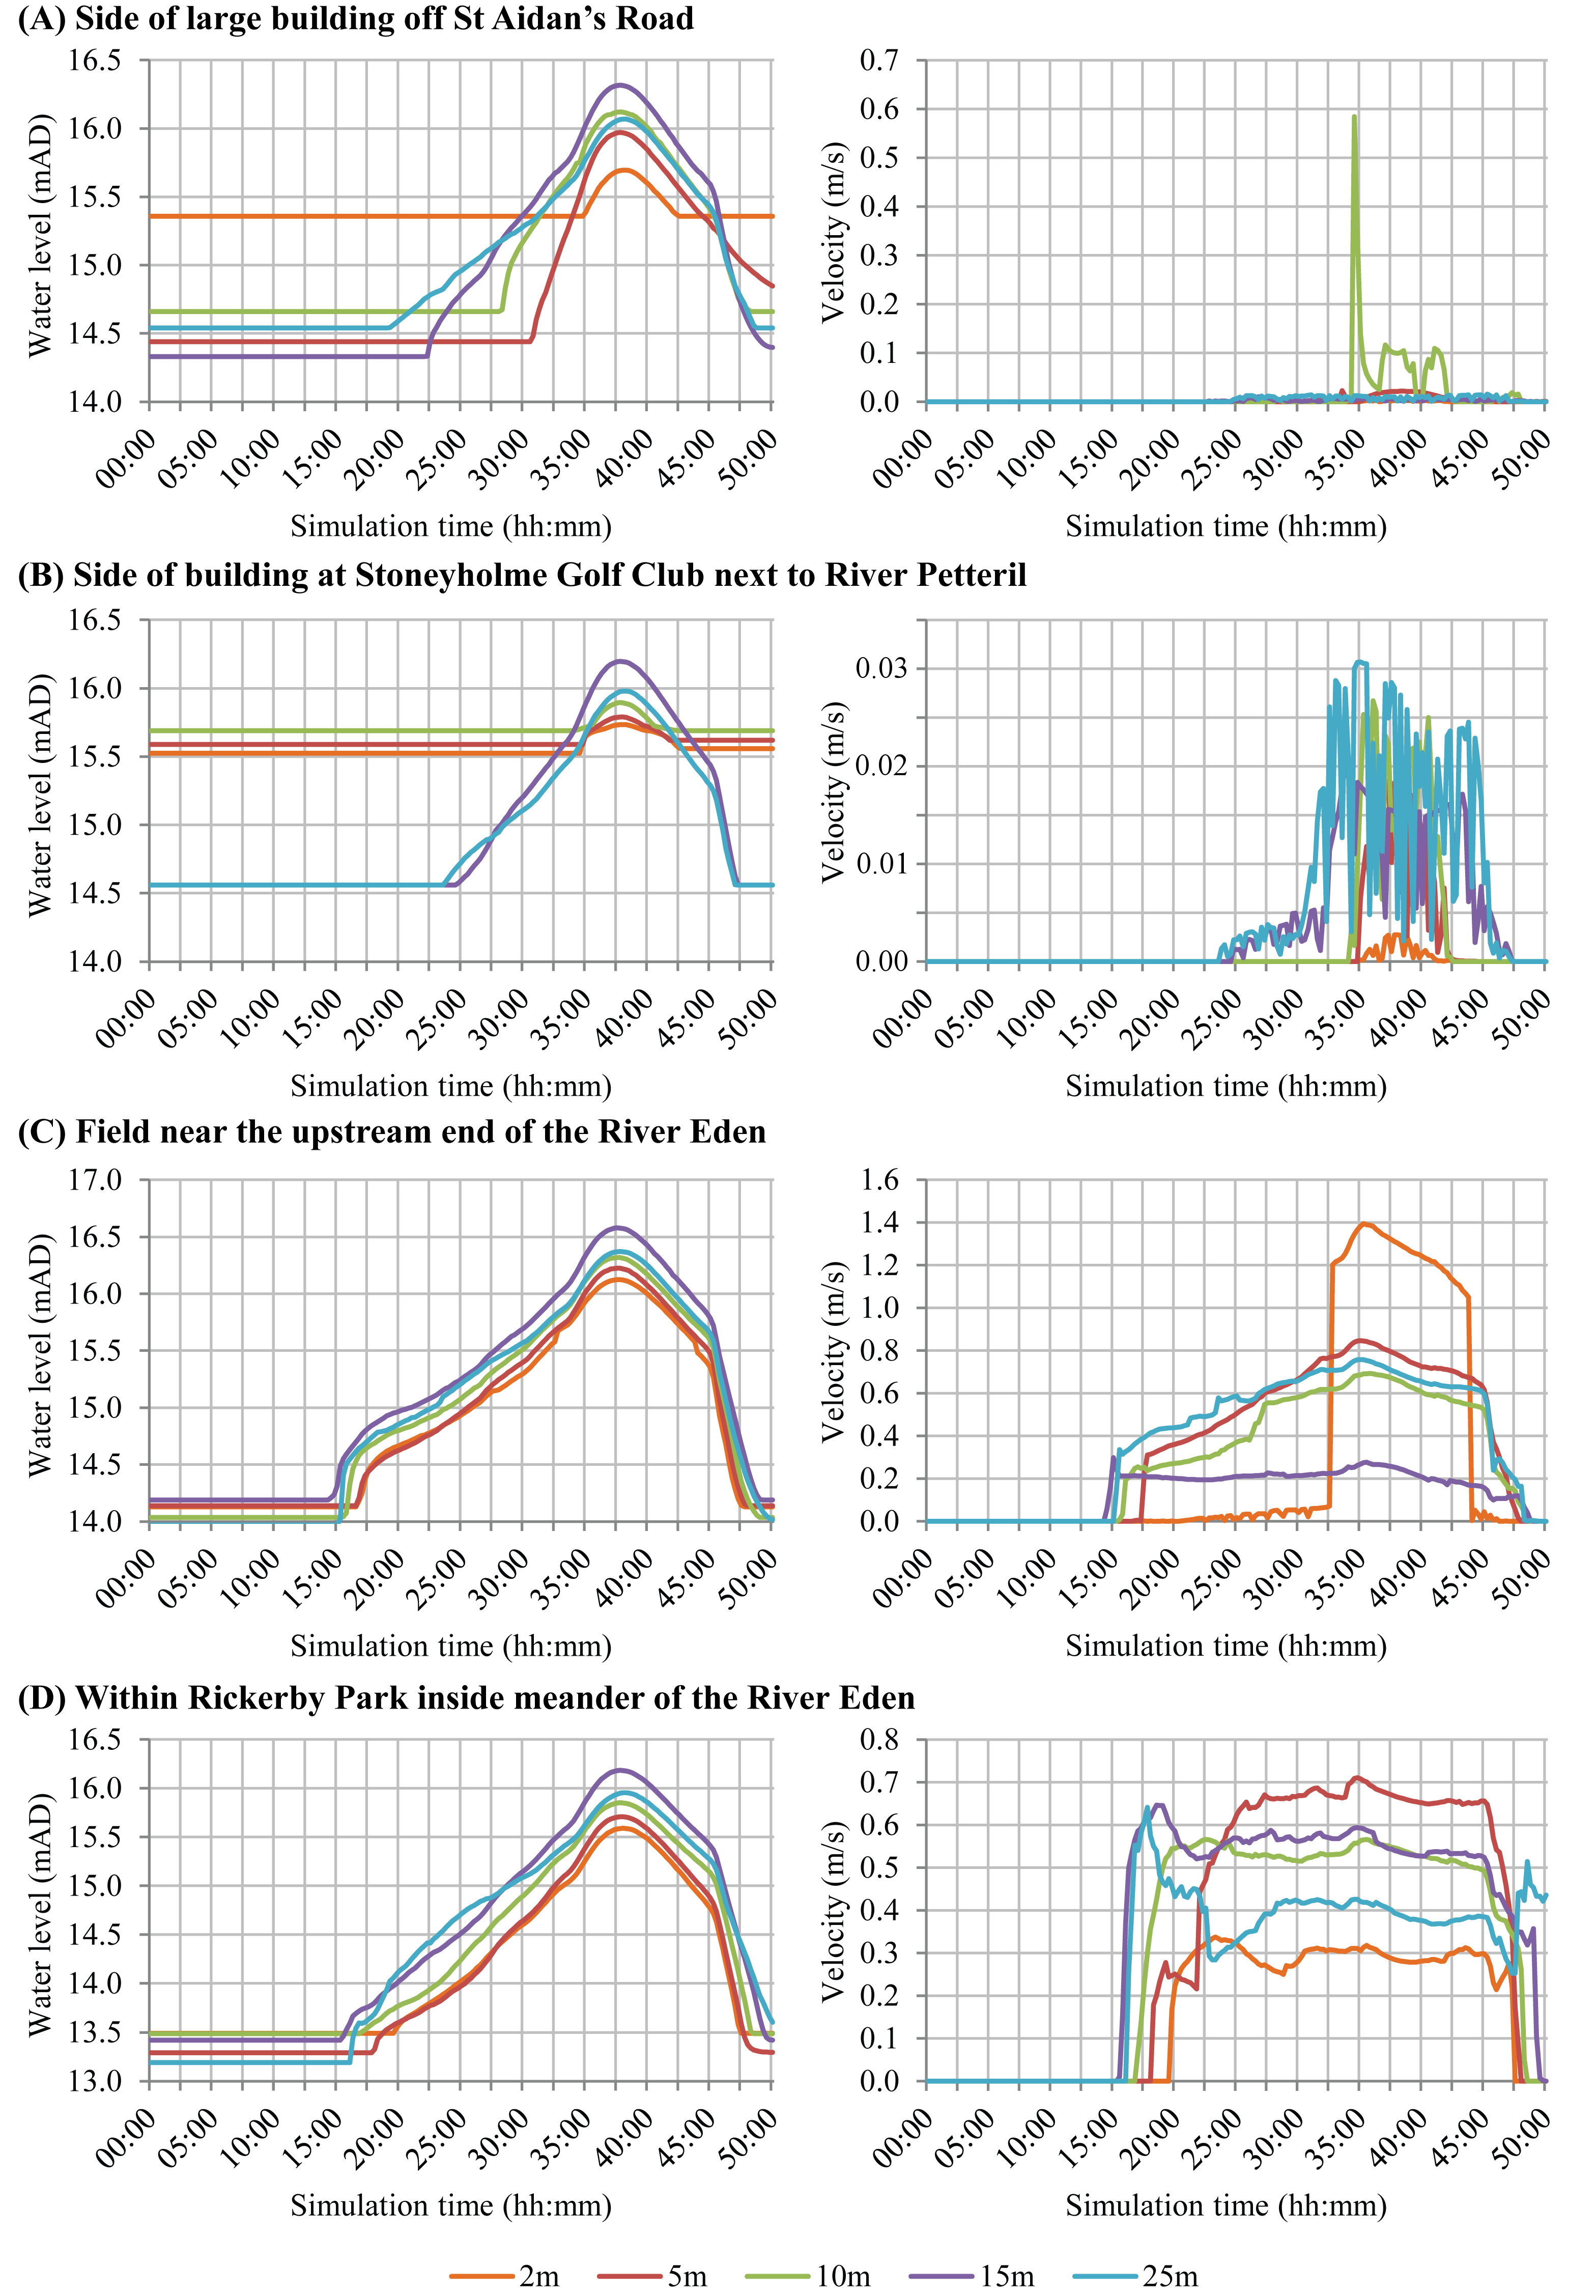
\includegraphics[width=0.93\textwidth]{carlisle-figures/Figure6.png}
	\caption{Water level and velocity plots with respect to simulation time for the four sample points identified in Figure \ref{CarlisleMap}, with fixed Manning's n of 0.04.}
	\label{TimeseriesPlots}
\end{figure*}

The value of \(C\) in equation \eqref{CFL} is taken to be 0.5 for all simulations of Carlisle, to be consistent, and accepting that some numerical diffusion may occur, but the errors present in the input datasets are likely far more significant. It is emphasised that model stability should be ensured for values up to 1.0 in idealised linear cases (as used for stability analysis), and the value selected is purely based on prior experience and analytical test cases with shocks and discontinuities \citep{Liang2009c}. Simulations were run at 5 different spatial resolutions: 2m, 5m, 10m, 15m and 25m. A downstream depth condition is imposed on the River Eden at the western edge of the domain, extrapolated from the nearby Sheepmount gauging station and thus negating its value as a further validation control. The performance of each simulation is evaluated with respect to the RMSE for the DGPS survey points, which are compared against the simulated water level for the nearest inundated cell by straight-line distance. A fit statistic \(F\) is assessed against the extent, 

\begin{equation}
	\label{FitStatistic}
	F (\%) = \frac{A - B}{A + B + C} \times 100,
\end{equation}

where \(A\) is the number of correctly predicted as inundated cells, \(B\) the erroneously predicted as inundated cells, and \(C\) the erroneously predicted as dry cells \citep[as in][]{Horritt2010}. It should be noted that this metric, although well-established, exhibits a slight preference among erroneous cells for under- rather than over-estimation, which could penalise coarse resolution simulations where terrain averaging has removed obstructions from the floodplain.

Floodplain and channel Manning's \(n\) were independently varied between the ranges of 0.02 -- 0.06 and 0.02-- 0.08 respectively at 0.01 intervals, requiring 35 simulations per resolution and 175 in total. Observations during and after the flood suggest that levels on the River Caldew upstream of a disused railway bridge were increased at least in part by debris trapped under a bridge, and that the gas works area initially flooded as a result of wall collapse \citep{EnvironmentAgency2006a,Fewtrell2011a}, which is not considered within the model. Accordingly the bias is not considered a good measure of model performance; RMSE and F are the two metrics considered to be most appropriate. A non-stationary response to calibration is found for different resolutions. Calibration of Manning's \(n\) is based on selecting the parameter pair giving the lowest RMSE against the DGPS points. This is the only uncertainty considered herein, however the hydrograph inputs used are the result of retrospective analysis of the event commissioned by the Environment Agency; a reasonable level of accuracy is hence assumed for the timeseries inputs. Selected river channel Manning's \(n\) were 0.060, 0.045, 0.020, 0.020, and 0.075 for resolutions 2m, 5m, 10m, 15m and 25m respectively. Floodplain values were 0.040, 0.050, 0.050, 0.020, and 0.020 in the same order. Maximum depths for the calibrated simulations are shown in Figure \ref{MaxDepths}, where it can clearly be seen that similar extents are attainable for all of the spatial resolutions considered herein. 

Timeseries plots of water levels and velocities at each resolution for the sample points shown on the map in Figure \ref{CarlisleMap} are displayed in Figure \ref{TimeseriesPlots}, for a uniform Manning coefficient of 0.04 for the domain including the channel. Where the water level is flat at the start of a simulation, this indicates the bed elevation of the cell which is hence dry. Velocity results vary significantly between different resolutions, however no data exist to validate velocities. Low velocities would typically be expected at point A, which is far from the watercourses and within a residential area with obstructions. Close to the River Petteril at point B, there is clear evidence that velocities vary greatly at coarse resolutions, not unexpected given that the river is less than 5m wide at this point; crucially however the time of inundation at this point is incorrectly predicted at 15m and 25m resolutions.  At point C the levels are in broad agreement across all resolutions, however a clear jump in velocities is observed at 2m resolution, which is a result of flow eventually overtopping a wall in this location only represented in high-resolution data. Levels are also in agreement at point D, however velocities vary across a range with no clear trend against grid resolutions. The 2m grid resolution consistently produces the lowest floodplain velocities, except in the case of point C as described.

\begin{figure*}[tpb]
	\centering
	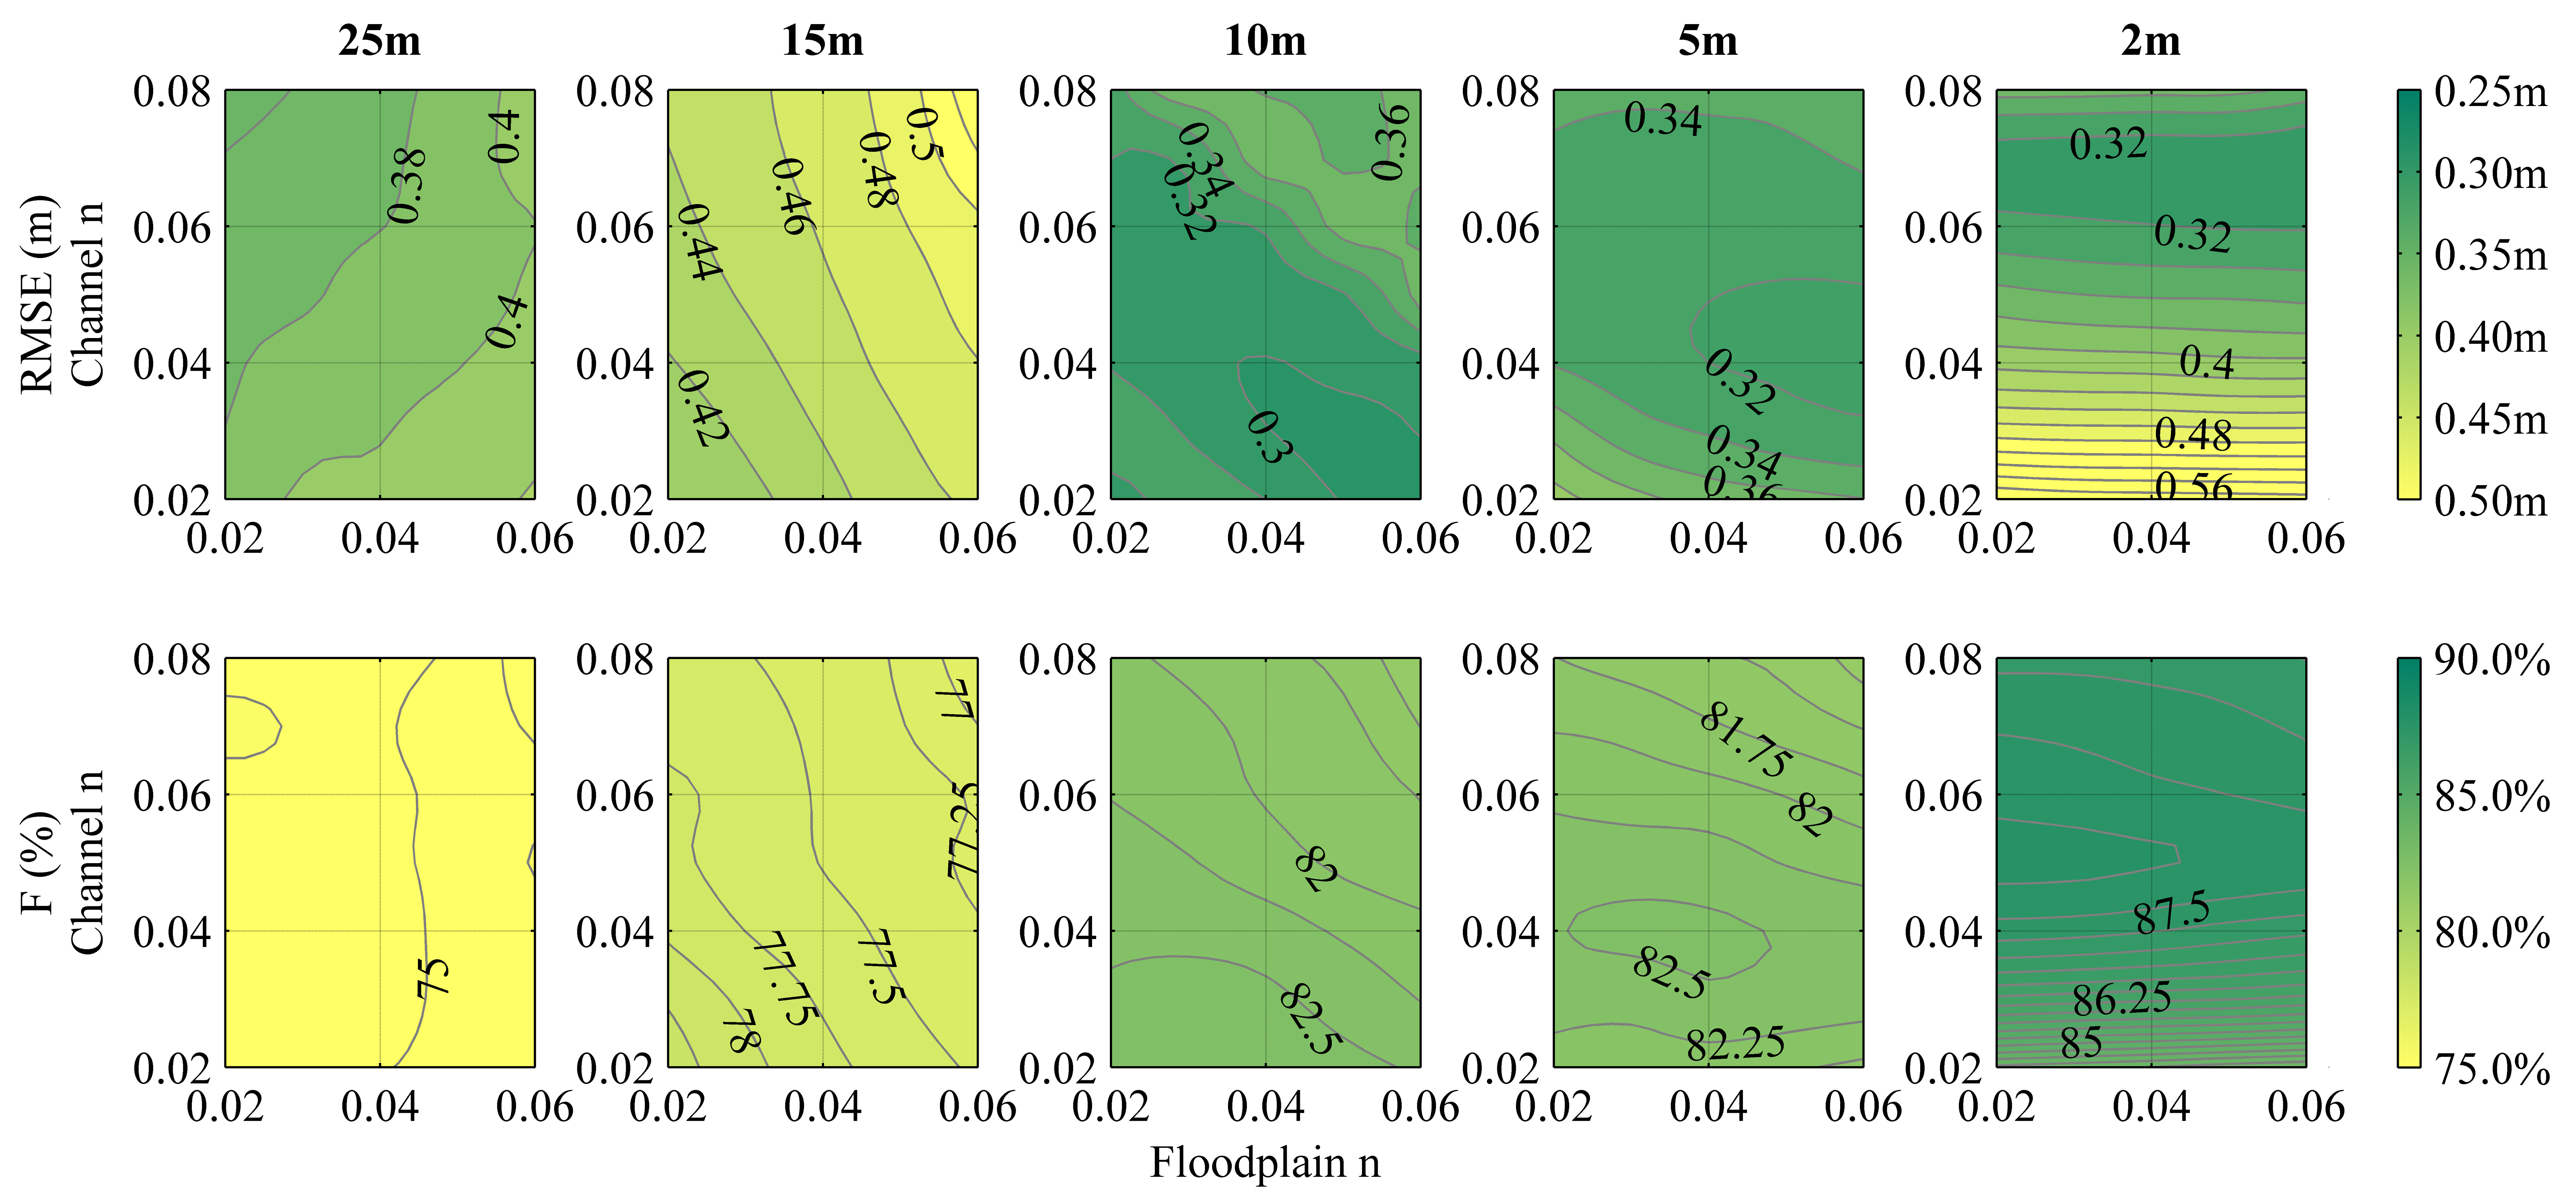
\includegraphics[width=1.0\textwidth]{carlisle-figures/Figure7.png}
	\caption{Parametric calibration for variations of Manning's n within the channel and floodplain.}
	\label{Calibration}
\end{figure*}

Further exploration of sensitivity to Manning coefficients yields interesting results. Contour plots for the biparametric calibration with the key performance metrics are shown in Figure \ref{Calibration}. Almost all of the simulations give an RMSE less than the estimated error in the DGPS measurements. At coarse resolutions optimum performance with respect to RMSE and F are not coincident. There is no consistent trend in the pattern of the optimal zones, as the resulting topography after interpolation can vary greatly at coarse resolutions owing to the size and positioning of buildings. For an increasingly fine grid, clear optimal zones emerge at 10m and 5m resolution, and by 2m only an optimal channel coefficient can justifiably be identified. For clarity at coarse resolutions no optimal zones could be found outside the calibration limits. Moreover the sensitivity changes in nature; higher resolutions show a decreasing sensitivity to the floodplain Manning's \(n\) and increased sensitivity for the channel. At 2m resolution sensitivity for the floodplain is so low that floodplain calibration barely influences the results and channel flows become the dominant factor, as confirmed by the lower velocities on the floodplain shown in Figure \ref{TimeseriesPlots} except at point C where a wall is eventually over-topped. This is not unexpected, velocities should be low for a fluvial inundation of this type, and given the meandering channel a high spatial resolution allows variations in flow characteristics within cross-sections to be properly considered.

\begin{figure*}[bp]
	\centering
	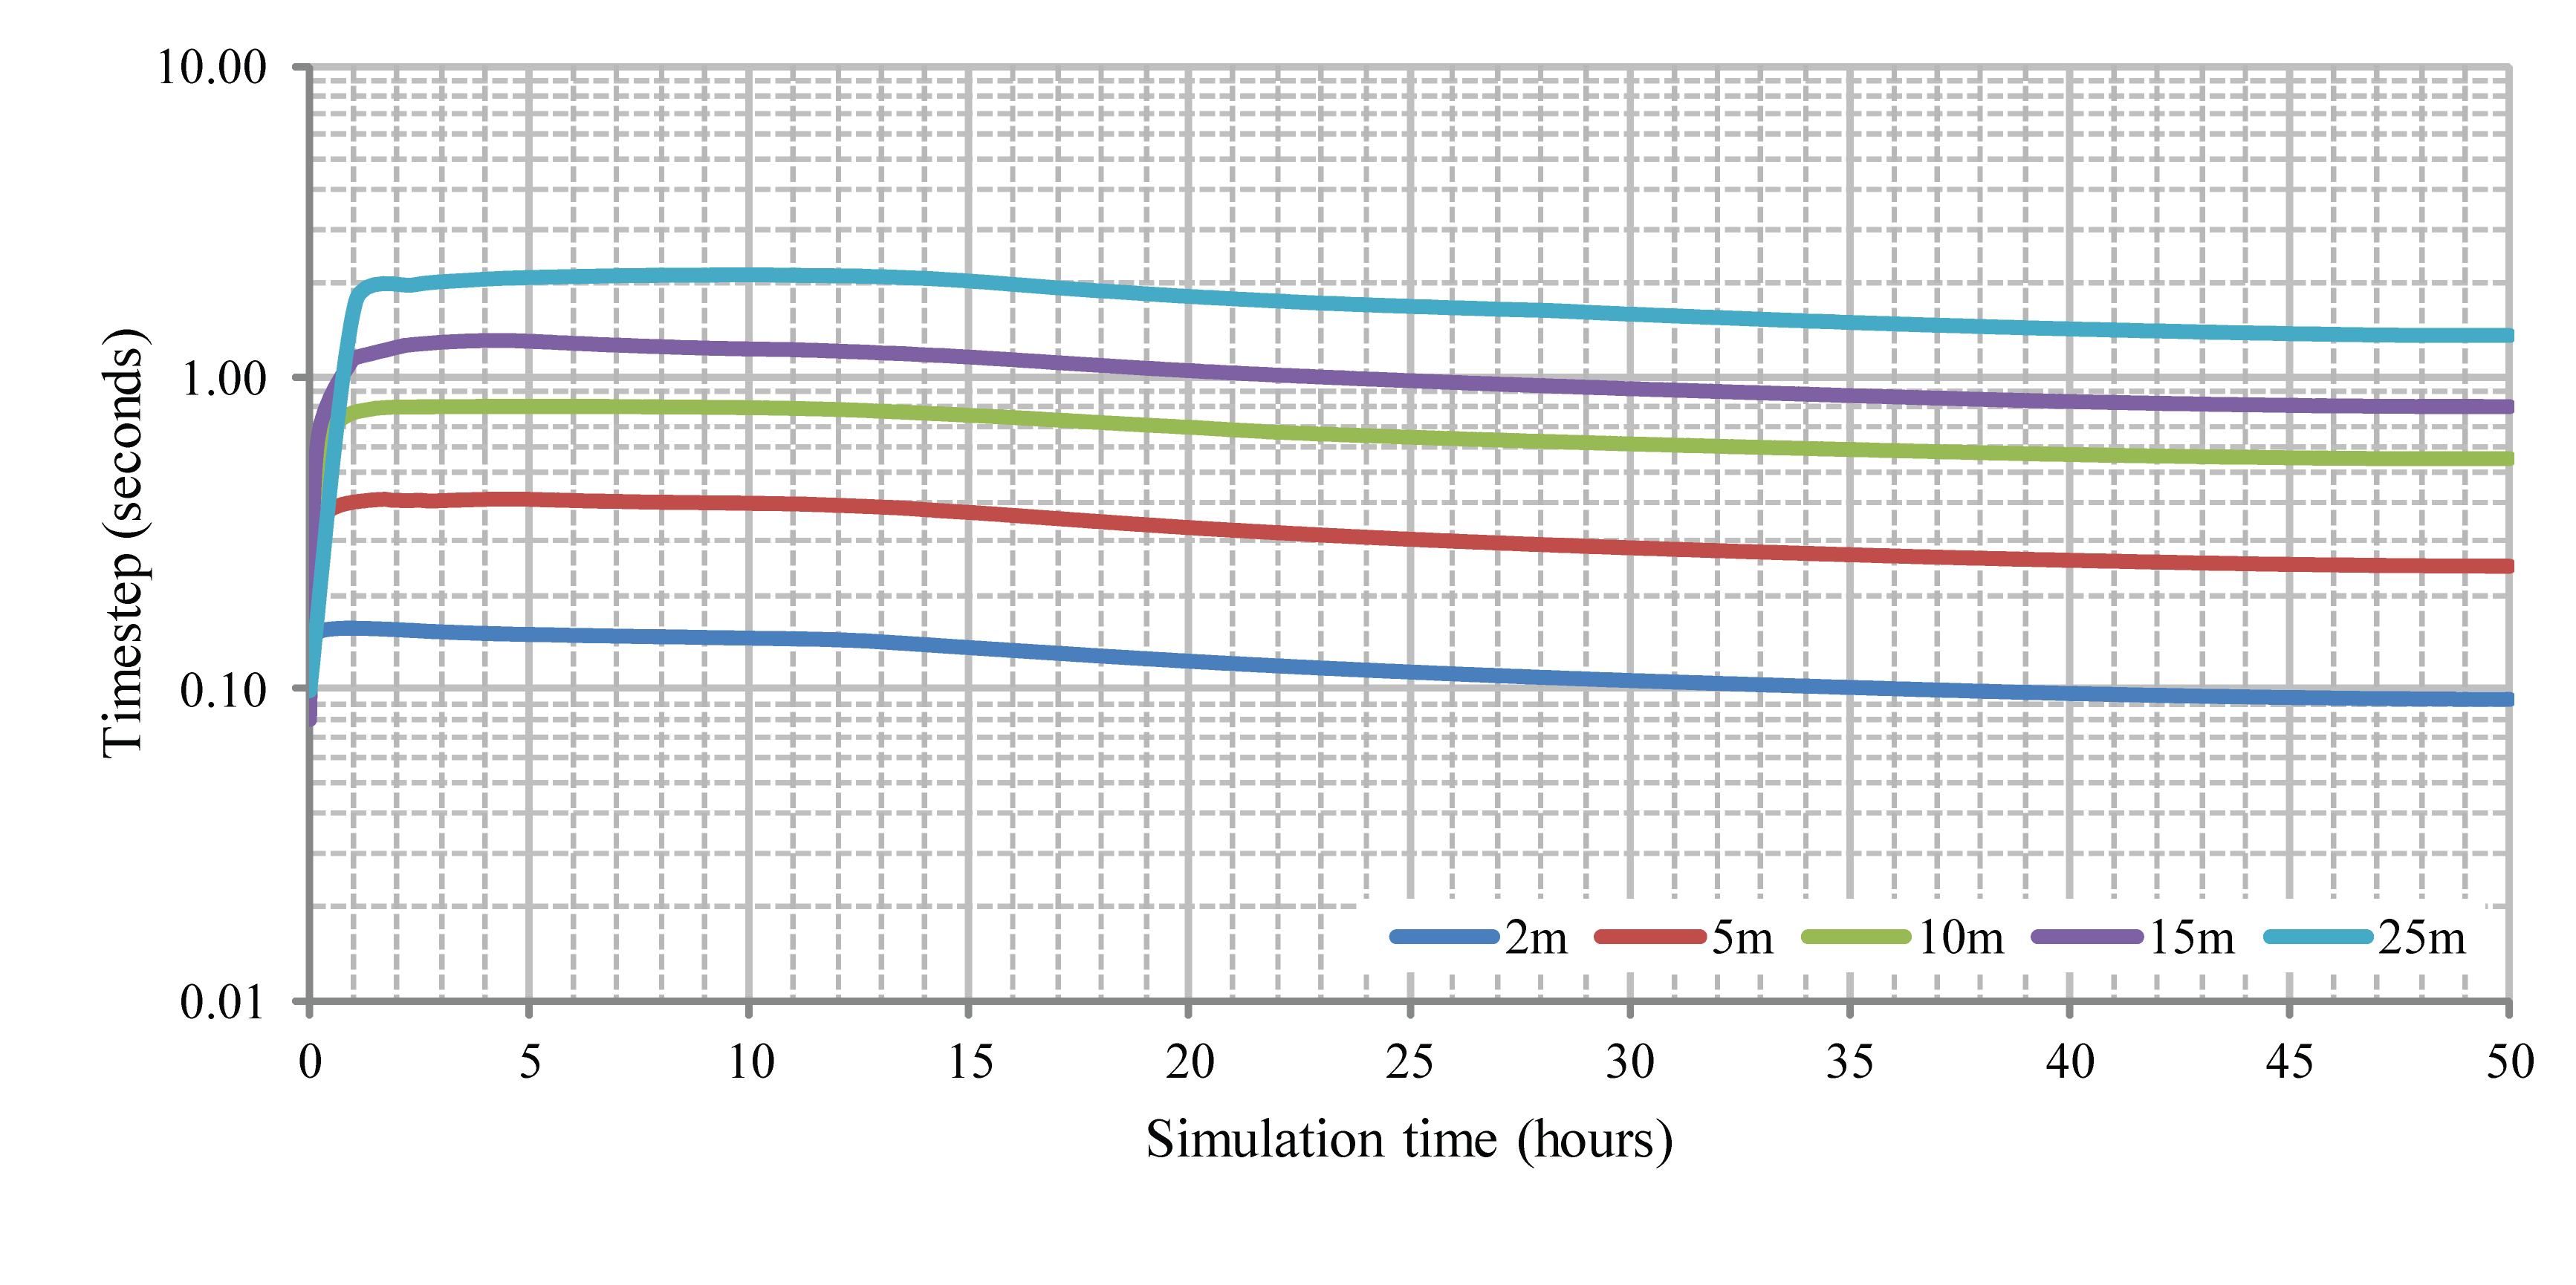
\includegraphics[width=1.0\textwidth]{carlisle-figures/Figure8.png}
	\caption{Model timesteps used throughout the 64-bit Carlisle simulations at different resolutions.}
	\label{Timesteps}
\end{figure*}

Closer examination of velocities at different intervals in the simulation shows that at coarse resolutions the flow is often circumventing the main channel due to the Cartesian grid and winding channel. Flow therefore enters the floodplain (especially in the meanders in the centre of Figure \ref{CarlisleMap} around point D) at a higher velocity, and the sensitivity to Manning's \(n\) is accordingly higher in these areas. If the low floodplain sensitivity were to hold more generally in the context of other flood events, there is clear potential for high-resolution hydrodynamic modelling with the full shallow water equations to improve accuracy in the simulation of hypothetical events, or statistically-derived scenarios. The combination of high grid resolutions and velocities in the main channel affect the timesteps shown in Figure \ref{Timesteps}, which can be as small as 0.093 seconds for the 2m simulation.

The reality however, is this event occurred close to the transitional zone of the River Eden, where slopes are minimal and the floodplain is relatively flat. Defence overtopping creates low velocities in such environments, where as water flows over the steep banks of the defences themselves, criticality is induced, and energy is lost soon after. It is essential therefore, to also consider sensitivity within the context of high flow velocities across the floodplain, such as in a catastrophic failure of the defences.

\subsection{Computational performance}

\begin{table*}[tpb]
\small
\centering
\caption{Simulation run-times for different devices, spatial resolutions and numerical precision (hh:mm:ss)}
\label{PerformanceResults}
\makebox[\linewidth]{
\begin{tabular}{llllllll}
\hline
			 		& 			& \multicolumn{2}{c}{NVIDIA Tesla M2075}			& \multicolumn{2}{c}{AMD FirePro V7800}			& \multicolumn{2}{c}{Intel Xeon E5-2609} 	\\
Resolution		 		& Cells		& 32-bit 		& 64-bit 		& 32-bit 		& 64-bit 		& 32-bit 		& 64-bit 	\\
\hline
25m					& 23,370		& 00:00:30	& 00:01:21	& 00:01:02	& 00:01:56	& 00:03:39	& 00:06:57 \\
15m					& 63,668		& 00:01:21	& 00:04:16	& 00:02:29	& 00:07:16	& 00:11:51	& 00:24:44 \\
10m					& 145,656		& 00:03:21	& 00:11:18	& 00:04:05	& 00:16:41	& 00:32:33	& 01:18:31 \\
5m					& 581,061		& 00:18:45	& 01:10:05	& 00:20:18	& 02:12:07	& 03:47:01	& 09:29:52 \\
2m					& 3,637,491	& 03:24:22	& 13:41:44	& 10:37:04	& \textit{\textgreater 40 hours}	& \textit{Not tested}	& \textit{Not tested} \\
\hline
\end{tabular}
}
\end{table*}

The time taken to simulate the first 50 hours of the event, long enough to obtain the maximum extent, is given in Table \ref{PerformanceResults}. By contrast, an NVIDIA Tesla M2075 intended for scientific computing reduces the run-time to less than 3.5 hours or 14 hours for 32- and 64-bit floating-point computation respectively. Free-surface levels and velocities are sufficiently small for this case to allow good numerical resolution and only minor differences in inundation extent when comparing 32-bit to 64-bit results. It must be emphasised that this is not true for the general case, and sensitivity analysis is always necessary before discarding 64-bit precision. It is suggested that the narrowing performance gap between NVIDIA and AMD devices with increasing resolution is a consequence of the overhead associated with launching a kernel, which becomes an increasingly small percentage of the total time. There are many factors influencing performance however. The AMD GPU is installed in a conventional workstation, and exhibits substantially reduced performance in simulations lasting more than an hour (i.e. 2m and 5m 64-bit), believed to result from hardware performance throttling because of high temperatures.

All simulations in Table \ref{PerformanceResults} were carried with using OpenCL, using all processing power and cores available for each device. Consequently even the processing time with the Intel Xeon E5-2609 CPU (quad-core with hyper-threading) represents a major reduction over many of the hydraulic modelling software packages currently used in industry, which offer no parallelisation or have been retrospectively parallelised in part using OpenMP \citep{Pender2010,Pender2013}. In such cases, where retrospective parallelisation is added, significant portions of code still execute serially and Amdahl's Law dictates that the serial portion of the program will govern the maximum reduction achievable in computation time; this limits performance increases. As expected for devices compliant with relevant IEEE standards for floating-point computation, there is no difference between the results obtained using the three different processing devices. 

As a purely indicative representation of the performance scaling achieved, the same numerical scheme programmed in FORTRAN95 and executed on a single core of the same CPU required 4.10 hours for the 10m 64-bit precision simulation. The software presented herein therefore reduces simulation times by approximately 3.1 times for the multi-core CPU and 21.8 times by using a high-end GPU for this simulation. This comparison with FORTRAN95 code should not be construed as precise; software performance on any processing device is a function of the programmer's skill, compiler used, degree of optimisation, memory access patterns, and numerous other factors. The magnitude of the speed-up with OpenCL for GPU devices is also seen to scale with increasing domain size, from 5.1 times at 25m to 8.1 times at 5m resolution, when comparing the Intel Xeon to the NVIDIA Tesla. Speed-up is dependent on a number of factors, but amongst the most significant is the proportion of dry cells; the overhead associated with launching a kernel and transferring data to registers for evaluation remains constant, but for dry cells kernels are permitted to exit early and this overhead is proportionally larger. Greater levels of speed-up relative to CPUs could be achieved for a larger domain with more immediate inundation (i.e. flash flooding), but likewise GPU computation may in fact be slower for very small domains at coarse resolutions.

\section{Hypothetical flooding in Thamesmead caused by defence failure}

The Thamesmead district of South London is located downstream of London's main flood defence, the Thames Barrier. The area is low lying but was heavily developed in the 1960s. Flood risk is posed by storm surges or a failure in the defence wall, with the area previously inundated in the North Sea Surge of 1953. A hypothetical breach in the defences is considered here, through which over 2,500,000m$^{3}$ of water enters the area with the hydrograph and entry point indicated in Figure \ref{Thamesmead_Conditions}. A 10-hour period is simulated, allowing the water to continue spreading through the computational domain.

\subsection{Model generation}

\begin{figure*}[p]
	\centering
	\begin{subfigure}[t]{0.5\textwidth}
		\centering
		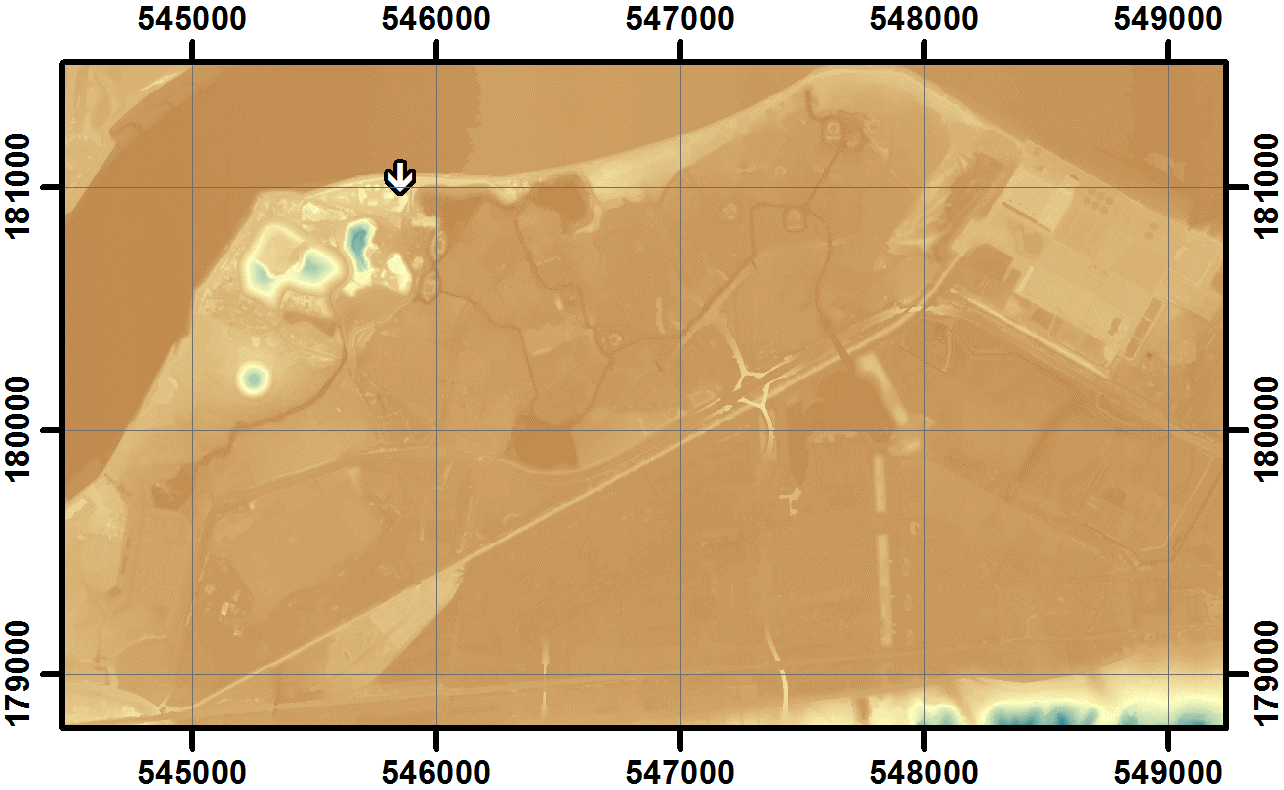
\includegraphics[width=1.0\textwidth]{heterogeneous-dev-figures/Thamesmead_DTM.png}
		\caption{Digital terrain model (DTM) and inflow location for Thamesmead}
	\end{subfigure}%
	~ 
	\begin{subfigure}[t]{0.5\textwidth}
		\centering
		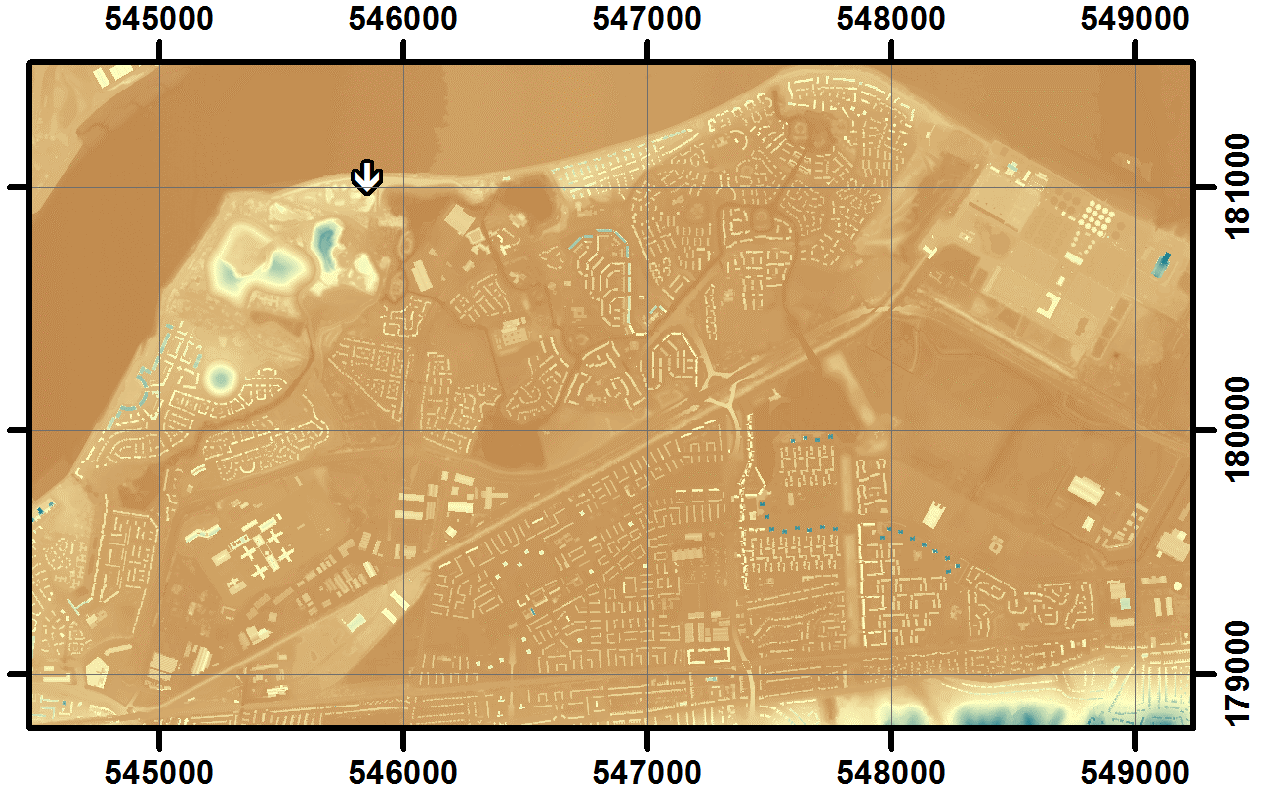
\includegraphics[width=1.0\textwidth]{heterogeneous-dev-figures/Thamesmead_DEM.png}
		\caption{Digital elevation model with buildings included (DEM) for Thamesmead.}
	\end{subfigure}
	
	\begin{subfigure}[t]{0.7\textwidth}
		\centering
		\includegraphics[width=1.0\textwidth]{heterogeneous-dev-figures/Thamesmead_Inflow.png}
		\caption{Volumetric discharge at the breach location.}
	\end{subfigure}
	\caption{Boundary conditions and topography used in Thamesmead simulations.}
	\label{Thamesmead_Conditions}
\end{figure*}
\begin{figure*}[p]
	\centering
	\includegraphics[width=1.0\textwidth]{heterogeneous-dev-figures/Thamesmead_10m_Comparison.png}
	\caption{Inundation results after a 10-hour period for the 10m resolution Thamesmead DTM used in \citet{Liang2010a}.}
	\label{Thamesmead_10m_Comparison}
\end{figure*}

The same hypothetical event is considered by \citet{Liang2008a}, \citet{Liang2010a}, and \citet{Vacondio2012}. These studies used a 10m resolution grid of 360,000 cells, whereby buildings and vegetation were removed from LiDAR altimetry data to create a digital terrain model (DTM). First, the simulation previously explored in literature with a 10m DTM is reproduced, in order to further validate the model. The inundation results are presented in Figure \ref{Thamesmead_10m_Comparison}, where only minimal disagreement can be identified against the results in \citet{Liang2010a}, which is effectively the same numerical scheme. This stems from differences in treatment of inflow boundary conditions for the new software, for which \citet{Liang2010a} applies imposes these on fluxes across cell boundaries, while the new software applies boundary conditions at the cell level.

The software presented herein allows us to go further. Updated datasets were created using a 2007 survey, and the resulting DTM and elevation model with buildings included (DEM) are shown in Figure \ref{Thamesmead_Conditions} at 2m resolution with 9,013,004 cells. As previously, a uniform Manning coefficient of 0.035 is applied across the domain. Cells within and north of the River Thames are excluded from computation. Transmissive boundary conditions are imposed at the domain edges. The final volume error is \textless0.1\% of the inflow volume. It can clearly be seen that a lesser flood extent is found with the new DTM in Figure \ref{Thamesmead_Inundation} for the same resolution. The updated terrain model depicts a deeper network of canals and lakes, offering increased storage.

Simulations were undertaken using both 32-bit and 64-bit floating-point arithmetic. Results presented are for 64-bit unless otherwise indicated. Whilst the average error in depth introduced by 32-bit arithmetic is small, the localised errors are in some cases unacceptably large. Errors were more pronounced at 10m resolution with the DEM; the average error exceeded 0.1m and the largest error was 0.98m. By contrast the average errors for all simulations at 5m and 2m resolution were \textless 0.01m. The magnitude of these errors is in part a function of the numerical scheme employed, where herein the free-surface level $\eta$ is used to represent cell states, to maintain depth positivity, while some numerical schemes achieve this through alternate means, potentially allowing greater precision when storing low depths. As an example, a depth of $0.001234$ is stored under IEEE 754 using 1 bit for sign, 8 bits for an exponent, and 23 bits for the integerial 'fraction' raised to the exponent to produce the actual value, i.e. $2^{-10} \times 1.2636159 \approx 0.001233999$; larger values such as the free-surface level limit the exponent, hence the fraction bits provide a lower numerical precision. Nonetheless, it would not be surprising if coarse resolutions are more sensitive to numerical resolution given the larger volume affected by the same change in depth. Further research is required.

\subsection{Effect of grid resolution and parameterisation}

\begin{figure*}[p]
	\centering
	\includegraphics[width=1.0\textwidth]{heterogeneous-dev-figures/Thamesmead_AllDepths.png}
	\caption{Inundation results after a 10-hour period using DEM and DTM at different spatial resolutions, and the minimum and maximum inundation extents with Manning values from 0.01 to 0.09.}
	\label{Thamesmead_Inundation}
\end{figure*}
\begin{figure*}[p]
	\centering
	\includegraphics[width=1.0\textwidth]{heterogeneous-dev-figures/Thamesmead_AllVelocities.png}
	\caption{Magnitude of velocities at 6 hours using DEM and DTM at different spatial resolutions. }
	\label{Thamesmead_Velocities}
\end{figure*}

The final extent and inundation depth for the three resolutions and two elevation models employed are shown in Figure \ref{Thamesmead_Inundation}. The building layout is unusual in Thamesmead, with numerous connected networks of buildings. Small tunnels and alleyways allow for pedestrian access, and the elevation models have been adjusted to ensure these are present as a flow pathway. These passages are small however, hence the buildings can be expected to reflect a large volume of the flow impacting them; this is confirmed by the results obtained. Inclusion of buildings results in an increased inundation in the west of the domain. Spatial resolution also has a substantial impact on the flood extent. Figure \ref{Thamesmead_Velocities} shows the magnitude of the velocities after six hours, with the highest velocities present at the highest resolutions where narrow gaps are clearly resolved, concentrating flow to alleyways and streets. As a consequence flood progression is more rapid at higher resolutions. In this case, coarse resolutions may result in underestimation of flood extent.

Additional simulations were run for each grid resolution with different Manning's $n$ values from 0.01 to 0.09 at 0.02 increments, giving 30 simulations in total. This allows the sensitivity to parameterisation to be assessed, representing an envelope of uncertainty which in the real-world may be street furniture, vegetation, and obstructions such as vehicles. The minimum and maximum extent of flooding after 10 hours across the calibration range is shown in Figure \ref{Thamesmead_Inundation}. As expected, a lower Manning's $n$ results in a larger area of inundation by the end of the simulation. Consistent with the findings of \citet{Yu2006}, coarser grid resolutions exhibit lower sensitivity to Manning's $n$, while there is a substantial range in final extent for both the DEM and DTM at 2m resolution. This is unsurprising given the higher localised velocities at fine grid resolutions. Low sensitivity to parameterisation at coarse grid resolutions is not a justification for using these resolutions however, as the difference in inundation from coarse to fine resolution grids far exceeds the scope of influence any parameterisation might have. Consequently there is a clear need for sub-grid scale representation of topographic features, dynamically adaptive grids, or use of high-resolution grids throughout. 

The high-velocity nature of this hypothetical event contributes to the higher sensitivity, in contrast to studies exploring slow fluvial floodplain inundation by overtopping of defences rather than breach. \citet{Fewtrell2011a} demonstrate that floodplain sensitivity is significant in both a LISFLOOD and ESTRY-TUFLOW simulations of the Carlisle 2005 flood, using a 25m grid. However a more detailed representation of the in-channel flow dynamics using a high resolution grid and shock-capturing scheme throughout is shown to decrease floodplain sensitivity to have very little effect with a 2m grid for the same event by \citet{Smith2015}, and as described previously in this chapter.  Evidently, high-resolution simulations alone are insufficient for flood risk analyses in defence breach situations, requiring comprehensive exploration of inundation with different parameterisations to fully assess the potential consequences for hypothetical and statistically-derived flood events. At its most extreme, the use of coarse grids and a single Manning's $n$ in broad-scale flood risk analysis could significantly underestimate the threat, as demonstrated by the marked differences in results obtained herein.

\subsection{Computational performance}

First, performance is considered for the 10m simulation, to allow comparison with other studies of the same scenario. \citet{Liang2008a} reports a run-time on a computer of that era, in excess of 4 hours, demonstrating the scale of the improvement in a relatively short period of time, even without leveraging GPU computing. The Thamesmead simulation involves approximately four times the number of cells, when compared to the Glasgow test case presented in Chapter \ref{chapter:NumericalValidation}, however the different nature of the event means many of the cells will be dry, thus calculation may shortcut in these cases. The performance results presented in Table \ref{ThamesmeadPerformance} again show a clear performance advantage for GPUs against CPUs, as expected. The inferior GPU is again faster in both 32- and 64-bit computation, suggesting the 360,000 cells remain insufficient to mask the GPU transfer and dispatch overheads. Despite the increased cell count, some simulations are faster for Thamesmead than Glasgow, suggesting the number of inundated cells is highly influential in performance results. Accordingly, pluvial flooding is expected to be among the most computationally demanding of scenarios.

\begin{table*}[tpb]
	\newcolumntype{R}[1]{>{\RaggedLeft\arraybackslash}p{#1}}
	\small
	\centering
	\caption{Simulation run-times for Thamesmead in minutes using three different processing devices at different resolutions and DEM or DTM.}
	\label{ThamesmeadPerformance}
	\begin{tabular}{p{0.1\textwidth}p{0.1\textwidth}p{0.15\textwidth}R{0.15\textwidth}R{0.15\textwidth}R{0.15\textwidth}}
		\toprule
		\raggedright{Cell elevations} & \raggedright{Spatial resolution (m)} & \raggedright{Floating-point arithmetic resolution} & CPU Intel Xeon E5-2609 & GPU AMD FirePro V7800 & GPU NVIDIA Tesla M2075 \\
		\midrule
		DTM		& 	10	&	32-bit 	&	10.53	&	0.73	&	0.83 \\
		&		&	64-bit 	&	23.50	&	1.88	&	2.40 \\
		& 	5	&	32-bit 	&	47.20		&	2.78	&	3.25 \\
		&		&	64-bit 	&	109.12	&	10.50	&	10.33 \\
		& 	2	&	32-bit 	&	636.72	&	40.43	&	40.20 \\
		&		&	64-bit 	&	\textgreater 1,800.00 	&	154.25	&	137.88 \\
		DEM		& 	10	&	32-bit 	&	10.57	&	0.77	&	0.85 \\
		&		&	64-bit 	&	10.87	&	1.92	&	2.35 \\
		& 	5	&	32-bit 	&	50.55	&	3.03	&	3.45 \\
		&		&	64-bit 	&	118.20	&	10.68	&	10.97 \\
		& 	2	&	32-bit 	&	675.18	&	40.73	&	40.20 \\
		&		&	64-bit 	&	\textgreater 1,800.00	&	147.62	&	137.70 \\
		\bottomrule
	\end{tabular}
\end{table*}

Total simulation times for a 10 hour period in Thamesmead with different processing devices are given in Table \ref{ThamesmeadPerformance}. The software presented herein takes advantage of all four CPU cores made available to it, giving a much more realistic comparison between the achievable performance of GPU and CPU devices than comparisons against single-threaded code which may not have been optimised. Multiple orders of magnitude speed-up should not be expected when comparing against optimised code, based on vendor-quoted performance figures \citep{Brodtkorb2012,Smith2013}; examination of device peak compute power in terms of floating point operations per second (FLOPS) reaffirms that such dramatic levels of performance boost are highly unlikely. The AMD device performs well in all of the simulations, at speeds which are comparable to NVIDIA, but retailing at a much lower price. For large domains with millions of cells it is possible to reduce simulation time to a fifteenth or less of the multi-core CPU equivalent for the software presented herein.

\section{Conclusion}

This chapter has presented a real-world application of the new computational techniques, providing accurate results consistent with observations taken after the event. However, when the same methods are applied to a defence failure event, in which high velocities are encountered on the floodplain instead of only the river channel, sensitivity becomes a far greater concern. There are a number of observations and limits to consider in future simulations.

\begin{itemize}
	\item Lowering the numerical precision to 32 bits provides a substantial performance benefit in this case, where velocities are low and flooding is gradual over a long period. However, in advance of a simulation one could not definitively say that 64-bit precision would not be required; even a gradual event may have short time periods where velocities are high, or the cumulative effect of the small errors could eventually create a much greater deviation; it is the author's opinion that the performance benefits of 32-bit processing cannot be leveraged without full sensitivity analysis conducted first.
	\item Parameterisation is not transferable between different grid resolutions, as might be expected. The Manning coefficient is used to factor energy loss not fully captured elsewhere in the model, most notably that of friction, but a more refined grid resolution should capture a greater proportion of the flow characterisations from the real world, hence the correction required should decrease for gradually-progressing floods. In reality, the extent of these losses is spatially-varying, thus the Manning's $n$ should be spatially distributed; an inaccurate simplification was used here to allow exploration without excessive numbers of parameters, where only the river channel and floodplain were differentiated for Carlisle.
	\item High-velocity flood events, such as those caused by defence failure, are extremely sensitive to both the grid resolution and parameterisation. Failure to use a high-resolution mesh could seriously underestimate flood risk, especially in urban environments where the built environment provides narrow flow corridors which can exacerbate flow velocities.
	\item Marked differences are observed by using a DTM versus a DEM with buildings included, whereas the reality probably lies somewhere in between (i.e. above a threshold height, windows and airbricks would be expected to convey water through a building).
	\item External factors such as hardware throttling (where performance is artificially reduced to manage temperature or power) are difficult to quantify, as they are controlled by proprietary systems and software.
	\item Clear benefits in the refinement of the flood event are seen when using high grid resolutions which capture the topographic complexity, however the simulation run-times even with high-performance GPUs are still long.
\end{itemize}

Considering the run-time at high resolutions, and the potential need to run multiple simulations across a range of parameterisations to fully capture a range of outcomes, further performance improvements are required. Increasing the number of processing devices used is considered next.

\chapter{Domain decomposition and multi-device computation}
\label{chapter:Decomposition}

Considering the city-scale application of a model for Carlisle in the previous chapter, city-scale simulation was achievable, but the time consumed remains too long for use in a real-time simulation or forecasting capacity. To derive further performance improvements, further capabilities are required, to leverage the processing power of multiple compute devices, instead of just one. This may take the form of a traditional supercomputer architecture, with high-speed low-latency network connections between powerful discrete computers with many cores, or ideally for flood simulation, with many GPU devices available. Consistent with the approach outlined previously, it is the intention here to create a computational method which could theoretically be applied to either of these systems.

Leveraging multiple processing devices for a single simulation is no simple task, when considering the complexities of managing multiple devices of mismatched computational power, focusing on different parts of the spatial domain, and potentially within a number of discrete computer systems, connected by a network. For this reason, very few software for flood simulation can provide this functionality, and to the author's knowledge, none of those commercially available for distribution, provide this capability. Acknowledgement should be given to JBA Consulting's JFlow-GPU, built upon the work of \citet{Crossley2009}, which offers some of this functionality, but is an internal tool, not available for general resale.

There are but a handful of existing studies in which multi-GPU simulations have been attempted, for flood simulation. The work described by \citet{Saetra2012} provides a starting point and was groundbreaking, presenting a similar approach to one described later in this chapter, where timesteps are exchanged between all processing devices, delivering major performance benefits for their examples with many millions of cells. In practice, many simulations do not contain that many cells, and the requirement is as much concerning high throughput in terms of overall duration, which is a more difficult problem. Similar findings are reported in \citet{Vinas2013} and \citet{Asuncion2016}, where large domains are required to improve the weak and strong scaling effects. Previous work by \citet{Sanders2010} is also similar to the approach adopted herein, but focused on hydrological modelling using CPU-based supercomputer architectures, rather than GPUs, although the principles are comparable. The intention here is to provide software capable of accelerating as broad a range of flood scenarios as possible, thereby providing a means of operation on traditional supercomputer architectures and smaller systems, by leveraging OpenCL and other open platforms.

It is also worthwhile acknowledging the extent to which future advances in technology might negate the need for complex domain decomposition implementations. Processor clock speeds have advanced negligibly throughout the last decade, as scale and temperature becomes a constraint. However, multicore processing is increasingly prevalent, including in mobile devices, and this has largely allowed background processing and foreground to be segregated through threading, for an improved user experience. The same trend can be expected in future years until a major advance in computer processor technology is achieved. Multicore processors typically have access to a single shared memory domain, and thus decomposition is not required in the manner described herein. It is likely nonetheless that high-resolution data will become ubiquitous, and detailed physically-based catchment-scale modelling should become increasingly prevalent; domain decomposition is likely to be necessary for catchment-scale modelling for many years to come.

\section{Principles of domain decomposition in explicit time-marching schemes}

The finite-volume scheme can be considered in the form of stencil operations, for which each cell is dependent on its neighbours for a first-order solution. This is ideally suited to the architecture of GPUs, as described in earlier chapters. Achieving expedient simulation is largely dependent on a small portion of the overall code, which undertakes the calculations for the time-marching scheme; this is essentially flux calculation and updating of the cell states, followed by a reduction algorithm to identify the maximum velocity in any cell across the domain, for the purposes of satisfying the earlier-described CFL condition. This dependency on neighbouring cells presents a problem, where a straight-forward splitting of the domain would move some of those neighbours to an entirely different device and therefore memory.

The timestep then presents a further problem. The CFL condition described in Equation \ref{CFL} governs the maximum timestep through which the simulation can be advanced for each iteration. In a domain decomposition situation therefore, there are two possibilities: coordinate the timestep using the maximum velocity encountered anywhere in the domain, including across all processing devices; or manage simulations in which each device progresses at a different pace, by predicting suitable synchronisation points for data exchange. The first of these cases is the simplest, but requires data be exchanged between device after each iteration completes.

\begin{figure*}[tpb]
	\centering
	\includegraphics[width=1.0\textwidth]{decomposition-test-figures/aob.png}
	\caption{Illustration of the available overlap buffer, showing a domain split in the middle, with four rows of cells duplicated into both domains, hence each time a full synchronisation occurs these rows may be substituted with data from the corresponding region of the other domain to correct any errors from the limited knowledge of neighbouring cells.}
	\label{AOB_Description}
\end{figure*}

Taking the simplest case, where it is possible to exchange data in each iteration, the CFL condition provides the useful advantage that a discontinuity or a wave may only progress the distance of one cell during one iteration, as this is the premise of CFL, and thus reason it provides stability. Where the domains for each processing device overlap, data may be exchanged along that border such that neighbour data is always available. A minor extension to this approach, would be to overlap the domain partitions by more than a single cell, so only timestep data is exchanged at every iteration, and cell data need only be exchanged at a point prior to when the availability of neighbours would be exhausted; this number of neighbours available between the area of interest and the end of the overlap zone, will be referred to as the available overlap buffer (AOB) hereafter. This concept is illustrated in Figure \ref{AOB_Description}, where four rows of cells represent the AOB. The lack of data on cell states outside the domain under consideration causes small errors to be introduced in each iteration, but the same row is simultaneously processed as part of the other domain, because of the overlap, allowing these errors to be corrected when cell state data is exchanged. The numbers in the figure illustrate the order in which the errors propagate, one row per iteration pursuant to the CFL condition. The blue region indicates cells regarded as free of these errors, hence authoritative data source.

For the second case, in which each decomposed fragment of the domain may run independently with its own timestep, any error arising in the solution at the extremities of the domain, because neighbour data lacks currency, will only propagate by one cell at a time. This allows these errors to be corrected, providing the AOB is not spent by the time data is exchanged between compute devices. In the event overlap is exhausted, a rollback to the last saved state is required. This is nonetheless dependent on the maximum time step being calculated after each iteration, making some host bus transfers inevitable but minimizing their size. The requirement for an overlap also means a model must consist many millions of cells before decomposition to multiple devices becomes a worthwhile pursuit, because the total number of cells is increased by the procedure.

\section{A multi-device multi-nodal implementation with decomposition}

The optimisations and techniques discussed so far, have focused on using the OpenCL programming framework, and therefore can take advantage of either CPUs or GPUs with a single codebase. This portion of the code is optimized in two ways. Firstly, the code is compiled just-in time before the simulation begins, allowing model-dependent constants (e.g. the grid resolution, constraints on time steps, and some parameterisations) to be incorporated within the model code directly. Secondly, the process is implemented as a simple sequential set of OpenCL kernels representing the stencil operation, with appropriate barriers incorporated where synchronization is required across the whole computational domain.

The underlying system drivers manage the vectorization for low-level optimization, and deployment of this code on the hardware available, which need not be limited to GPUs but could also include hybrid-style processors (APUs) and IBM cell processors. Data is transferred to the device's own DRAM memory (see Figure \ref{CPUGPUArchitecture}) before computation begins, and transferred back as infrequently as possible, allowing for status updates and file-based storage of results. Transferring both instructions and large volumes of data across the host bus is far from desirable, and would represent a major bottleneck in the process if undertaken too frequently. However, as the total domain size increases, the delay introduced by latency across the host bus, as a proportion of overall computation time, becomes a diminishing portion. This presents an opportunity for domain decomposition, but only for instances where the problem size is sufficient to justify frequent data transfer.

\begin{figure*}[tpb]
	\centering
	\includegraphics[width=1.0\textwidth]{mpi-figures/sync-levels.png}
	\caption{Representation of the synchronisation levels, from work groups, to device domains, servers, and the overall domain spread across several computational nodes.}
	\label{Software_Sync_Levels}
\end{figure*}

This code is further developed, to support simulations across multiple GPUs using a domain decomposition technique, and across multiple systems through an implementation of the Message Passing Interface (MPI) standard \citep{MPI2009}. A separate CPU thread is used to manage each compute device, accepting some idle resource for a short period of time, for example in a tidal inundation model an entire sub-domain could be dry before the wave arrives. The general form for the multiple levels of data synchronisation is shown in Figure \ref{Software_Sync_Levels}, where data is exchanged between discrete computer systems using MPI, and within a single computer system, a separate CPU thread is used to coordinate for each device, with each allocated its own memory space.

The message passing interface (MPI) is a software standard for communication between processes operating either on the same machine, or connected via a network. It is commonly applied in supercomputing, where Infiniband, a communication standard capable of achieving throughput $\gtrapprox120$ GBit/s and latency $\lessapprox0.5$ microseconds, or comparable network speeds allow these messages to be passed with great speed and minimal latency, and the algorithms associated with some operations can in some cases be processed and assisted by network hardware, such as a reduction to find the largest or smallest value from those held by each node. There are a number of implementations of the MPI standard, many of which are open-source; herein, MPICH (\url{https://www.mpich.org/}) is adopted. There are numerous similarities between the functionality afforded by MPI, and that which exists in the OpenCL 1.2 standard, such as the commands to send and receive from memory buffers, and initiate barriers where all concurrent programs must wait for all others to reach the same point, for synchronisation. In the case of MPI over networks or between processes, even though extremely high speeds may be available, for applications which exchange large volumes of data on a regular basis, there is likely a limit beyond which no further performance gain can be achieved, in part because of the overheads of dealing with each of these operations, as a proportion of the productive processing time.

Owing to the speed constraints of the PCI bus, the means of transferring data from the main system memory to peripheral devices such as GPUs, these exchanges are computationally expensive, and so to reduce the frequency required, it is not necessary to exchange data after every time step, provided there is a sizeable overlap between the two sub-domains. 

\section{A temporally-decoupled implementation for decomposition}

The unproductive period while a processing device is consuming less than its full capacity while waiting for other elements to complete, is known as blocking, and is largely unavoidable. The issue comes when scaling simulations to use hundreds of processing devices, where not only is blocking required on a regular basis, it becomes a major complexity for the whole system, albeit one which can largely be handled by the algorithms and routines provided by MPI. The greatest source of blocking in the implementation described thus far in this chapter, is the exchange and identification of an appropriate timestep, to guarantee numerical stability. It follows then, that if timesteps need not be synchronised globally across the whole system, there is an opportunity to reduce blocking operations. 

The reality is slightly more complicated however: decoupling the timesteps between fragments of the whole domain, could lead to large disparities between the timesteps used, which are primarily a function of the depth and velocity in the fragment. A tidal inundation simulation for example, could have swathes of the domain initially completely dry, therefore requiring a single iteration to advance the simulation by the same amount as a hundred iterations for the fragment containing the sea, constrained by the CFL condition. The method that follows therefore, does not seek to remove the blocking, but merely reduces the amount of unproductive processing. Hypothetically, with some clever management of the simulation, by removing these unproductive iterations from the process other operations could take place instead. More than one fragment of the total domain could be assigned to a single processing device, such as large areas with minimal inundation, which would benefit from the scheme exiting early when dry cells are detected; this is a step further than the implementation described herein goes, but may be an opportunity for the future.

\begin{figure*}[tpb]
	\centering
	\includegraphics[width=1.0\textwidth]{mpi-figures/mpi-flowchart.png}
	\caption{Simplified representation of the processes involved in a temporally decoupled implementation, in which domain states may need to be reverted if synchronisation is not possible.}
	\label{Software_MPI_Flow}
\end{figure*}

In order to decouple the timesteps, an appropriate point in the future needs to be identified, at which the data may be exchanged. At this point, all domain fragments must be at the same point in time for the simulation. Calculation of an appropriate synchronisation point in the future is no simple task, and must be an estimate.

The approach adopted for determining an appropriate synchronisation point is:

\begin{itemize}
\item if the overall simulation time has progressed by $< 10^{-5}$ seconds, or the last known batch did not deliver any successful iterations, then revert to running a single iteration as synchronisation or an error may be imminent; otherwise
\item subject to the caveat, that the proposed synchronisation point should not be less than one timestep (per the CFL constraint calculated during the previous run) in the future, unless this would exceed a required point (i.e. when output files should be written to disk, or the simulation should terminate); then the synchronisation point is the current simulation time, plus the average timestep for each iteration since the last synchronisation, multiplied by the number of cells in the buffer, and the user-configured percentage of the buffer to consume.
\end{itemize}
This should provide a point likely to leave some of the buffer free (per the configuration), but this is not guaranteed, as the previous batch may not be representative of future flow conditions.

The performance achievable is highly sensitive to the user-configured spare AOB, where setting this value too low will result in an excessive number of rollbacks for the entire domain state, every time shocks and major variations in flow conditions are encountered, but too high will fail to fully utilise the processing power available, with potentially redundant cycles depending on the method employed for queueing iterations on the processor. There is also a coordination overhead associated with these calculations, and pausing elements of the simulation while a proposal is calculated at each node, and the lowest of these identified from all of the domains in a simulation. The above method is considered na\"ive, and could likely be improved with further tuning options, or a degree of adaptivity to deal with varying flow conditions, such as in a defence failure, where volatility in wave speeds is concentrated immediately following the failure.

If the AOB is exceeded, a rollback is required. Following each successful batch, the cell state data is transferred in its entirety from the processing device to the host device, which is oftentimes unused (apart from when output files are required) but necessary in case of rollback. A rollback entails copying the host-side cell state data back to the processing device, overwriting the current simulation time, and scheduling a timestep calculation using these previous cell states, before further fluxes are calculated. The rollback is required on all processing devices, hence the procedure is treated as a blocking operation, where no device will schedule further flux calculation until all devices have reported they are ready. Consequently, rollbacks are extremely expensive operations, especially when the coordination is across network devices.

A final consideration with temporal decoupling, especially in progressive flood events or tidal scenarios, is one subdomain may require considerably more iterations than another. Each iteration contributes a degree of numerical dispersion, resulting from both the numerical scheme employed, and the rounding of floating-point values under the IEEE-754 standard methods \citep{InternationalOrganizationforStandardization2011}. This is often not a cause for concern, but in some simulations, such as the sloshing parabolic bowl considered in Chapter \ref{chapter:NumericalValidation}, the cumulative effects can be significant. The different magnitude of numerical dispersion could potentially induce shocks at the seam of each subdomain, hence judicious and conservative application is required when employing this method.

\section{Software structure}

Considering all aspects of the domain decomposition, numerical scheme, and heterogeneous processing, the implementation of this software in a manner sustainable for further development becomes of paramount importance. The software is implemented as object-oriented code, which is illustrated in Figure \ref{Software_Class_Final}. Full implementation details and additional information may be found within the code and associated comments  (\url{https://github.com/lukessmith/hipims-ocl}). In general terms, the software is structured:

\begin{figure*}[p]
	\centering
	\includegraphics[width=1.0\textwidth]{mpi-figures/class-diagram.png}
	\caption{Simplified representation of the software structure, showing classes and some of their relationships.}
	\label{Software_Class_Final}
\end{figure*}

\begin{itemize}
	\item A model class (\texttt{CModel}) which provides access to all domain data and configuration for a simulation, which may be associated with an executor (i.e. the OpenCL executor for the work herein) for mapping to processing devices, and the MPI manager for internodal communication.
	\item An MPI manager (\texttt{CMPIManager}), which holds information concerning all of the nodes involved in the simulation, such as its devices and hostname, for logging and coordination purposes, within \texttt{CMPINode} instances.
	\item An executor controller (\texttt{CExecutorControl}) which is only used for OpenCL herein, but could potentially be expanded for other high-performance computing frameworks (e.g. CUDA) with some work, although much of the underlying numerical scheme code is OpenCL-specific. The \texttt{CExecutorControlOpenCL} instance provides access to the processing devices on the machine, as \texttt{COCLDevice} instances. For any specific simulation, a bespoke program is created (with model-specific constants compiled in) and managed through \texttt{COCLProgram}, with the code elements accessed and scheduled by \texttt{COCLKernel}, and memory on the processing device marshalled by \texttt{COCLDevice}. These latter classes also interpret OpenCL errors raised, and help ensure resources are cleaned up when no longer required.
	\item A number of utility classes called upon elsewhere in the program (per the programming paradigm of composition over inheritance), used for reading the XML file format (\texttt{CXMLDataset}), comma-delimited files (\texttt{CCSVDataset}) used for timeseries data, raster datasets (\texttt{CRasterDataset}) which are then handled by the GDAL library, logging to the console and files (\texttt{CLog}) and OS-independent timing of operations (\texttt{CBenchmark}).
	\item A base class for all domains, which is used also for MPI simulations, where a domain may actually exist and be controlled by another node within the network, but all nodes require an awareness of domains across the network to be able to synchronise data. Domains which exist locally are addressed by \texttt{CDomain}, and the only Cartesian domain type, currently the sole implementation (\texttt{CDomainCartesian}). Where domain decomposition exists, links are automatically created, and managed using \texttt{CDomainLink}, which extracts data from the domain where the overlap exists, and broadcasts this information across MPI to the relevant target nodes.
	\item All local domains have a \texttt{CBoundaryMap} which manages all types of boundary condition (uniform, spatiotemporally varying, and cell-specific). Each type of boundary has its own management class, responsible for loading the timeseries and spatial data, and provisioning memory on the processing device for this to reside in. This detail is omitted from Figure \ref{Software_Class_Final}.
	\item A scheme implementation, which may be first- or second-order, is managed by the \texttt{CSchemeGodunov} and \texttt{CSchemeMUSCLHancock} class (which inherits the first-order elements as a base, then supplements the additional computational steps). The scheme class is responsible for managing the time-marching, determining when data should be exchanged and written to disk, and the scheduling of work to the relevant processing devices.
\end{itemize}

A final consideration within the software design, is to ensure each device is managed by its own thread, allowing concurrent execution of the management processes, and thereby avoiding any slowdown of the heterogeneous element of the simulation.

\section{Validation and testing of the domain decomposition algorithms}

\begin{figure*}[tbp]
	\centering
	\includegraphics[width=0.92\textwidth]{decomposition-test-figures/screenshot-remote.png}
	\caption{Screenshot of the console output during a simulation using MPI between two servers with four GPU devices each.}
	\label{TestResult_Screenshot_8Domain}
\end{figure*}

The software's ability to decompose domains and synchronise data correctly between them, at the appropriate time, has been tested repeatedly during use. However, for the purposes of software testing, a limited number of identical processing devices were available, hence performance figures reported herein will use a maximum of three processing devices, all of which have identical specifications. Simulations involving up to eight processing devices were tested successfully, as shown in Figure \ref{TestResult_Screenshot_8Domain}, where two servers with four GPU devices each are used for a single simulation.

\subsection{Lake at rest}

The same test and parameterisations as found in Chapter \ref{chapter:NumericalValidation} are used here, however with a variety of grid resolutions. Whilst this test should not produce any movement of the water levels, it nonetheless requires flux calculations in all cells except the island in the centre (which is dry). It is therefore a useful performance test.

\begin{figure*}[p]
	\centering
	\includegraphics[width=0.85\textwidth]{decomposition-test-figures/static-lake-topography.png}
	\caption{Bed topography used for the static lake test with three devices, in which a tint has been applied to each of the subdomains to show the zones of overlap.}
	\label{TestResult_WellBalanced_Decomposed_Domains}
\end{figure*}
\begin{figure*}[p]
	\centering
	\includegraphics[width=0.85\textwidth]{decomposition-test-figures/static-lake-depth.png}
	\caption{Bed topography and depth after 10 minutes resulting from the static lake test with three devices, in which a tint has been applied to each of the subdomains to show the zones of overlap.}
	\label{TestResult_WellBalanced_Decomposed_Depth}
\end{figure*}
\begin{table*}[p]
	\small
	\centering
	\caption{Simulation run-times with different numbers of NVIDIA Tesla K40 devices, for the well-balanced property test, using the first-order Godunov-type and second-order MUSCL-Hancock schemes (hh:mm:ss)}
	\label{PerformanceResults_MultiGPU_WellBalanced}
	\begin{tabular}{p{0.15\linewidth}p{0.3\linewidth}p{0.1\linewidth}p{0.15\linewidth}p{0.15\linewidth}}
		\hline
		\multicolumn{5}{c}{\textbf{Performance results for well-balanced test (hh:mm:ss)}} \\
		\hline
		Resolution		 	& Productive cells					& Devices	& First-order	& Second-order	\\
		\hline
		8.0m				& 15,625 ($125 \times 125$)			& 1			& 00:00:01		& 00:00:01	\\
		&									& 2			& 00:00:01		& 00:00:01	\\
		&									& 3			& 00:00:01		& 00:00:01 	\\
		\hline
		4.0m				& 62,500 ($250 \times 250$)			& 1			& 00:00:02		& 00:00:02	\\
		&									& 2			& 00:00:02		& 00:00:02	\\
		&									& 3			& 00:00:02		& 00:00:02	\\
		\hline
		2.0m				& 250,000 ($500 \times 500$)		& 1			& 00:00:07		& 00:00:09 	\\
		&									& 2			& 00:00:05		& 00:00:06	\\
		&									& 3			& 00:00:06		& 00:00:07  \\
		\hline
		1.0m				& 1,000,000 ($1000 \times 1000$)	& 1			& 00:00:43		& 00:01:01	\\
		&									& 2			& 00:00:27		& 00:00:36	\\
		&									& 3			& 00:00:22		& 00:00:29	\\
		\hline
		0.5m				& 4,000,000 ($2000 \times 2000$)	& 1			& 00:05:14		& 00:07:45	\\
		&									& 2			& 00:02:46		& 00:04:02	\\
		&									& 3			& 00:02:10		& 00:03:02	\\
		\hline
		0.25m				& 16,000,000 ($4000 \times 4000$)	& 1			& 00:41:02		& 01:01:21	\\
		&									& 2			& 00:20:55		& 00:31:12	\\
		&									& 3			& 00:16:02		& 00:23:08	\\
		\hline
	\end{tabular}
\end{table*}

When the domain is divided in two, the island is also divided, hence the processing load for each device should be identical. Division of the domain into three creates a central domain, in which the island resides, where fewer cells require flux calculation; accordingly, one device has a reduced workload, but the software should be capable of addressing this, and where timesteps are synchronised between domains, the slowest domain becomes the governing factor. Figure \ref{TestResult_WellBalanced_Decomposed_Domains} shows the domain divided into three.

No movement in the water level is expected, for any duration of time. This behaviour is confirmed in the results shown in Figure \ref{TestResult_WellBalanced_Decomposed_Depth}, which confirms the synchronisation procedures in the software are correctly mapping the overlapping cells during data transfer.

The domain is $1000 \times 1000m$, and ten rows of cells form the overlap between each fragment of the domain, meaning at least an additional five rows per device for each division introduced. Grid resolutions from $8.0m$ to $0.25m$ are evaluated, and timesteps are synchronised between domains for this test. Accordingly, each new device introduced increases the total number of cells requiring computation.

The total run-times are given in Table \ref{PerformanceResults_MultiGPU_WellBalanced}. With regard to strong scaling, for higher resolutions, a marked decrease in run-time is shown for an increasing number of processing devices. The scaling is not linear, with the run-time at $0.25m$ resolution approximately $2.56\times$ lower for first-order, and $2.65\times$ for second-order. This is expected: the domain sizes are not sufficiently large to alleviate the overhead associated with synchronisation, most notably the requirement to transfer the timestep information across the host bus following each iteration of the scheme. The slightly larger factor of improvement for second-order corresponds to the increased workload within the scheme itself, and thus the smaller proportion of time consumed by simulation coordination. This is consistent with the findings of \citet{Saetra2012}, where the total domain size exceeded $40M$ cells before near-linear scaling was observed. Using multiple GPUs only seemingly becomes worthwhile in this case for $16M$ cells and beyond, with very little benefit at lower numbers of cells. This poses a problem for many simulations which are applied today, for which the problem is often the duration of the simulation rather than the number of grid cells, for which multiple processing devices can offer little benefit.

\subsection{Moving wet-dry fronts}

The sloshing parabolic bowl test, previously used in Chapter \ref{chapter:NumericalValidation} provides a different problem for the software to address. In this simulation, the velocities are constantly changing, and when the domain is divided, different CFL constraints are likely to exist in each component. Considering the requirement for extremely large numbers of cells to fully leverage the processing power available, this simulation uses grid resolutions ranging from $20m$ to $1.25m$ for a $10,000 \times 10,000m$ domain, hence up to $64M$ cells.

Results at different times during the test simulation using the MUSCL-Hancock scheme, with two domains, are shown in Figure \ref{TestResult_ParabolicBowl_2O_Decomposed2}. These clearly correspond to the expected results previously shown for a single domain in Figure \ref{TestResult_ParabolicBowl_2O}. Results using both explicit timestep synchronisation, and the decoupled forecasted method produce near-identical results, with some minor differences in water level but no change to the overall behaviour. These results demonstrate the software's capacity to correctly simulate the complex condition of constantly moving wet-dry fronts, even when these conditions occur along the divide between two subdomains. Simulations were also conducted using a first-order scheme, for performance comparisons only, as the results are known to deviate significantly from the analytical solution due to numerical diffusion. 

\begin{figure*}[tpb]
	\centering
	\begin{tabular}{cc}
		\includegraphics[width=0.4\textwidth]{decomposition-test-figures/parabolic-bowl-2O-2D-depth-300s.png} &
		\includegraphics[width=0.4\textwidth]{decomposition-test-figures/parabolic-bowl-2O-2D-depth-600s.png} \\
		(a) 300s &
		(b) 600s \\[6pt]
		\includegraphics[width=0.4\textwidth]{decomposition-test-figures/parabolic-bowl-2O-2D-depth-900s.png} &
		\includegraphics[width=0.4\textwidth]{decomposition-test-figures/parabolic-bowl-2O-2D-depth-1800s.png} \\
		(c) 900s &
		(d) 1800s \\[6pt]
		\includegraphics[width=0.4\textwidth]{decomposition-test-figures/parabolic-bowl-2O-2D-depth-3600s.png} &
		\\
		(e) 3600s &
	\end{tabular}
	\caption{Representative times for the parabolic bowl results for comparison against Figure \ref{TestResult_ParabolicBowl_2O}, with the domain decomposed down the middle, and the depths and bed topography tinted to reflect the processing device responsible.}
	\label{TestResult_ParabolicBowl_2O_Decomposed2}
\end{figure*}
\begin{table*}[p]
	\small
	\centering
	\caption{Simulation run-times with different numbers of NVIDIA Tesla K40 devices, for the sloshing parabolic bowl test, using the first-order Godunov-type and second-order MUSCL-Hancock schemes (hh:mm:ss) with 64-bit floating point}
	\label{PerformanceResults_MultiGPU_SloshingBowl}
	\begin{tabular}{p{0.15\linewidth}p{0.3\linewidth}p{0.1\linewidth}p{0.15\linewidth}p{0.15\linewidth}}
		\hline
		\multicolumn{5}{c}{\textbf{Performance results for sloshing parabolic bowl (hh:mm:ss)}} \\
		\hline
		Resolution		 	& Productive cells						& Devices	& First-order	& Second-order	\\
		\hline
		20.0m				& 250,000 ($500 \times 500$)			& 1			& 00:00:01		& 00:00:18	\\
		&															& 2			& 00:00:01		& 00:00:15	\\
		&															& 3			& 00:00:01		& 00:00:13 	\\
		\hline
		10.0m				& 1,000,000 ($1000 \times 1000$)		& 1			& 00:01:05		& 00:01:54	\\
		&															& 2			& 00:00:42		& 00:01:09	\\
		&															& 3			& 00:00:39		& 00:00:57	\\
		\hline
		5.0m				& 4,000,000 ($2000 \times 2000$)		& 1			& 00:07:44		& 00:13:39 	\\
		&															& 2			& 00:04:14		& 00:07:18	\\
		&															& 3			& 00:03:43		& 00:05:45  \\
		\hline
		2.5m				& 16,000,000 ($4000 \times 4000$)		& 1			& 00:59:58		& 01:47:07	\\
		&															& 2			& 00:31:27		& 00:55:58	\\
		&															& 3			& 00:27:06		& 00:43:45	\\
		\hline
		1.25m				& 64,000,000 ($8000 \times 8000$)		& 1			& 07:56:11		& \textit{N/A}	\\
		&															& 2			& 04:05:55		& 07:14:53	\\
		&															& 3			& 03:27:58		& 05:36:40	\\
		\hline
	\end{tabular}
\end{table*}

It was not possible to simulate the $1.25m$ grid using the MUSCL-Hancock scheme on a single device, as the NVIDIA Tesla K40 has insufficient memory to hold the intermediate data. The ability to run simulations exceeding the capacity of a single device is nonetheless an additional benefit of the domain decomposition approach. There is evidence that at the tens of million cell scale, strong scaling is approaching linearity. The first-order run-time is reduced by $48.4\%$ using two devices instead of one. The scaling is less ideal for three devices, but an even larger domain would likely achieve scaling improvements. Consistent with the previous results in this chapter, decomposition is shown to only be worthwhile for extremely large domains.

\section{Performance of forecasted and coupled implementations}

The results presented thus far focus on simulations in which the timesteps are synchronised between all domains, which is the simplest and most reliable method of domain decomposition available in the software. It is also possible to temporally-decouple the simulations, so their timesteps are independent and data is synchronised at a forecasted point in the future. The aforementioned tests in this chapter all produced comparable (although not identical) results using both methods of synchronisation; the differences are derived from the different timesteps and number of iterations, and consequent minor difference in the numerical diffusion. 

\begin{table*}[p]
	\small
	\centering
	\caption{Simulation run-times with forecasted and coupled runs of first 10 minutes of the sloshing bowl test using the second-order scheme (hh:mm:ss)}
	\label{PerformanceResults_MultiGPU_ForecastMethods}
	\begin{tabular}{p{0.15\linewidth}p{0.1\linewidth}p{0.35\linewidth}p{0.15\linewidth}}
		\hline
		\multicolumn{4}{c}{\textbf{Performance comparison for methods of synchronisation (hh:mm:ss)}} \\
		\hline
		Resolution		 	& Devices	& Synchronisation				& Run-time \\
		\hline
		5.0m				& 2			& Coupled timesteps				& 00:01:14 	\\
							& 2			& Forecasted synchronisation	& 00:01:37	\\
		\hline
		2.5m				& 2			& Coupled timesteps				& 00:08:58	\\
							& 2			& Forecasted synchronisation	& 00:11:14	\\
		\hline
		1.25m				& 2			& Coupled timesteps				& 01:10:00	\\
							& 2			& Forecasted synchronisation	& 01:27:43	\\
		\hline
	\end{tabular}
\end{table*}

Simulation run-times for the first 600 seconds of the sloshing parabolic bowl simulation are given in Table \ref{PerformanceResults_MultiGPU_ForecastMethods}, in which the forecasted method is markedly slower than timestep synchronisation. There are a number of reasons for this: the forecasted synchronisation point means sometimes kernels are scheduled which cannot perform flux computation, but the overhead associated with running the kernel remains present; some of the simulation may be repeated because of a rollback, if the forecast was inaccurate; and the additional time taken to download an entire copy of the cell state data after each successful batch of scheme iterations. 

For simulations in which the workload is comparable in all domains (e.g. the tests used herein, or a pluvial rainfall event in which all cells are engaged in computation), then timestep synchronisation is recommended. The forecasted method potentially may provide performance benefits in select cases, such as balancing hardware resources which do not have equal computational power, or when the domain is decomposed such that one domain contains a far greater proportion of wet cells, or far higher depths, than the remaining domains.

\section{Conclusions}

This chapter presented the background and algorithms associated with domain decomposition in the new software, where a single domain may be split into a number of horizontal components, with each addressed by a different processing device. This allowed simulations exceeding the memory available on a single device, and reduced the run-time of simulations, in some cases achieving near-linear run-time reduction for the number of devices added.

\begin{itemize}
	\item Many of the simulations used in practical engineering applications at present, are too small to fully benefit from domain decomposition to multiple heterogeneous devices. In particular, long duration simulations as opposed to large spatial extents, cannot be accelerated using the decomposition methods herein.
	\item Decomposed elements of a domain may share a single timestep or be independent, by predicting a point in the future to synchronise data, however there are but a handful of circumstances in which the latter would be a more expedient option, as the additional complexity involved carries a performance cost.
	\item Results obtained through the decomposition methods are near-identical (to at least three significant figures) to those from a single processing device, and do not inhibit the capabilities of the numerical scheme discussed in Chapter \ref{chapter:NumericalMethods}.
	\item Simulations which require processing power exceeding that which may be provided by a single server, can use the new software to leverage multiple servers, using MPI for internodal communication.
\end{itemize}

This chapter only considered the methods, and validity of results obtained therewith, for domain decomposition. The approach must therefore be applied to a real-world case, which would not be feasible to simulate without the assistance of multiple heterogeneous processing devices.
\chapter{Application of multi-device computation to a detailed city-scale surface-water flood simulation}
\label{chapter:ScaleEffects}

The domain decomposition methods provided in the last chapter allow simulations to be accelerated considerably when compared to traditional single-core CPU-bound software. This capability allows the spatial extent and resolution of simulations to be pushed beyond the realms previously considered, and as such creates new research questions surrounding the limits of data presently available, predictive capability of the models, and future data requirements.

This chapter considers a real-world pluvial flood event, by leveraging all of the data which could be obtained, and processing power available to the author at the time of writing.

\section{Flooding in Newcastle during June and August 2012}

\begin{figure*}[tpb]
	\centering
	\includegraphics[width=1.0\textwidth]{newcastle-pluvial-figures/radar-rainfall-totals.png}
	\caption{Rainfall totals derived from rainfall radar for the flooding in Newcastle and the surrounding region, on 28 June 2012.}
	\label{Newcastle_Pluvial_RainTotal}
\end{figure*}

One of the most publicised floods in the UK during 2012 occurred in Tyne and Wear on 28th June 2012, during a month where many parts of the country were battered by short-duration heavy rainfall and thunderstorms over already saturated ground \citep{JBARiskManagement2012}. A supercell storm hit the city of Newcastle upon Tyne in North East England and the surrounding area at approximately 15:00, leaving the worst impacts to coincide with the peak evening commute. The effects of up to 50mm of rainfall during two hours were dramatic: Newcastle Central Station was flooded and the surrounding railway lines flooded or damaged by landslides; underground stations on the area's light rail network were flooded; grade-separated (i.e. overlapping infrastructure with different elevations) junctions connecting the city to all of the major arterial roads were flooded; and bus services were suspended in some areas. Many were stranded with no way to get home. More than 300 properties were flooded internally, and damage to highways alone in the Newcastle area was estimated at up to £8 million \citep{NewcastleCityCouncil2013}. Rainfall intensity varied greatly, both spatially and temporally across the city, but in some instances an intensity exceeding 200mm/hr was recorded for a short duration \citep{EnvironmentAgency2012a}.

The flooding manifested from a quasi-stationary convective storm, typified by thunder and a thick substantial layer of cloud, greatly reducing visibility and creating night-like conditions. The pattern was such that only a narrow band suffered the highest rainfall accumulations, whilst ten kilometres to the east or west received very little. The highest accumulations were believed to be slightly to the east of the city centre, as can be shown from the radar totals in Figure \ref{Newcastle_Pluvial_RainTotal}.

\section{Data sources and model generation}

Initially, two simulations have been carried out with a 2m resolution, one covering 36km$^{2}$ of Newcastle central area and another covering 400km$^{2}$ of Tyne and Wear, which respectively involve $~8$ million and $100$ million computational cells. The extent of the larger of these domains is shown in Figure \ref{Newcastle_Pluvial_DomainExtent}, along with the location of photos solicited from the public. Due to the flashy nature of the flood event, no organized field measurements are available for model validation, hence crowd-sourced data was relied upon; these were in the form of textual descriptions, photographs and videos submitted by the public.

\begin{figure*}[tpb]
	\centering
	\includegraphics[width=1.0\textwidth]{newcastle-pluvial-figures/20km-domain-extent.png}
	\caption{Model extent for the 20 $\times$ 20km area around Tyne and Wear used to simulate flooding on 28 June 2012.}
	\label{Newcastle_Pluvial_DomainExtent}
\end{figure*}
\begin{sidewaysfigure}
	\centering
	\includegraphics[width=1.0\textwidth]{newcastle-pluvial-figures/radar-rainfall-sequence.png}
	\caption{Rainfall radar timeseries centred on Newcastle upon Tyne, showing intensities for the 28 June 2012 event.}
	\label{Newcastle_Pluvial_Radar}
\end{sidewaysfigure}

Domain inputs used for all simulations were extracted from UK Met Office C-band rainfall radar (NIMROD) from 12:00 UTC to 18:00 on 28 June 2012, shown in Figure \ref{Newcastle_Pluvial_Radar}. Comparison of radar data against tipping bucket raingauges on the ground suggests good agreement. The Tyne and Wear model covers the full extent with highest rainfall totals, for the flood event considered as per rainfall radar. Specifically, this spans from $(415000, 555000)$ to $(435000, 575000)$ on the British National Grid (OSGB36). Bed elevations are in effect a digital elevation model, obtained by superimposing buildings from the first-pass return of an Environment Agency LiDAR survey atop a filtered terrain model, blended with OS Terrain 5 data where LiDAR coverage was lacking. This produces an elevation model where buildings are present, as important in determining the direction of flow, but vegetation which would provide minimal flow resistance (e.g. trees and bushes) are omitted. Buildings are not superimposed in the case of bridges and similar overhead structures, where a viable flow pathway is likely to exist beneath. Whilst imperfect insofar as there may be locations where flow could exist on two different levels within the same location, this is considered to be a practical compromise.

Generation of the elevation model was automated by processing OS MasterMap Topography Layer data to identify building outlines and overhead structures. A Manning coefficient of 0.2 is used across the whole domain; sensitivity testing suggested minimal effect on flood depths for this model. Cells which would ordinarily contain water, including ponds and rivers, were disabled from computation to allow the simulation to focus entirely on pluvial flooding processes. Domain decomposition is activated on the basis of synchronising timesteps.

The drainage network is not explicitly represented within the model, however as a substitute, a 12.5mm/hr drainage loss rate is applied to all cells, a figure which slightly exceeds the 10\% annual exceedance probability 2-hour duration event against which drainage infrastructure must be designed to withstand \citep{DMRB2016}, but is similar to the recommendations in Table 2 of BS EN 752:2008. This is also near-identical to the 12mm/hr "national average" rate adopted for England's surface water flood risk mapping \citep{EnvironmentAgency2013}.

Following the flood event, members of the public were invited to contribute photos and their respective locations for flooding through a dedicated website, which was advertised across the region using local television and radio. Social media activity from Twitter was also archived for analysis, which is examined in the next chapter. Areas worst affected were surveyed under instruction from the local council, with a questionnaire asking which areas of their property and the neighbouring infrastructure were affected. Briefing reports on the hydrology and its consequences were prepared by the Environment Agency and \citet{EnvironmentAgency2012a,NewcastleCityCouncil2013}.

\section{Results}

The software successfully provided results for the simulation, which are now considered against the evidence available for the actual extent of flooding, and discrepancies further analysed.

\subsection{Computational performance}

The simulations conducted were able to provide near real-time or faster prediction, for the six-hour period simulated, by leveraging multiple GPU devices. A sufficient number of identical processing devices was not available, hence two models of NVIDIA devices were mixed. These were four NVIDIA Tesla K40 and two K80 devices, where the latter is a single board which behaves as two discrete devices, so this manifests as eight devices in total. It is believed that further performance improvements could be achieved with the same software, if greater resources were made available, hence there is potential for these highly detailed simulations to be used in a predictive capacity in the future. The full performance details are given in Table \ref{PerformanceResults_MultiGPU_Newcastle}.

\begin{table*}[tbp]
	\small
	\centering
	\caption{Simulation run-times with different numbers of NVIDIA Tesla K40 and K80 devices, for the simulation of the Newcastle upon Tyne pluvial flood event on 28 June 2012, using different domain sizes}
	\label{PerformanceResults_MultiGPU_Newcastle}
	\begin{tabular}{p{0.15\linewidth}p{0.08\linewidth}p{0.15\linewidth}p{0.2\linewidth}p{0.15\linewidth}}
		\hline
		\multicolumn{5}{c}{\textbf{Performance results for simulations of the area surrounding Newcastle upon Tyne}} \\
		\hline
		Zone		 		& Area					& Resolution (cells)	& Devices						& Runtime (hh:mm:ss)	\\
		\hline
		Tyne and Wear		& $400 km^{2}$			& 2m (100,000,000)		& 4$\times$K40M 2$\times$K80	& 06:01:00				\\
		City centre			& $34 km^{2}$			& 2m (8,805,496)		& 4$\times$K40M 2$\times$K80	& 01:01:22				\\
		\hline
	\end{tabular}
\end{table*}

\subsection{Ability to reproduce large-scale flood features}

\begin{figure*}[tbp]
	\centering
	\includegraphics[width=1.0\textwidth]{newcastle-pluvial-figures/centre-depth-lettered.png}
	\caption{Extract of flood depths for a subsection of the simulation results, focusing on the centre of Newcastle upon Tyne.}
	\label{Newcastle_Centre_Depths}
\end{figure*}

The locations of a subset of photos received, alongside simulation results showing maximum depths, are shown in Figure \ref{Newcastle_Centre_Depths} for a small area of the city ($\approx$ 2 $\times$ 2km). It is clear there is strong agreement between the locations of the crowd-sourced photos and flooding. On the A167(M) Central Motorway, at points A and F it can be seen that dips in the road for intersections have suffered from serious flooding, which is an unfortunate consequence of the transport infrastructure design in Newcastle, and reinforces that some settlements are more exposed to the risk of pluvial flooding. Some of the longest overland flow pathways converge at point C on the Newcastle University campus, and G near The Gate entertainment complex, and these are clearly visible as some of the highest depths. Points E and D highlight some of the limitations of the approach, with the football pitch at E seeing exaggerated flooding because infiltration and drainage is inadequately represented, and a large pool appearing at D where in fact the railway line goes underground, but topographic data obtained did not reflect this. Point B represents a pedestrian passageway under a major road, which is accurately represented and was known to flood, however the road above is not represented and was also flooded. As a whole, the simulation results provide an accurate representation of the flooding which occurred in June 2012, albeit with scope for improvements by manual intervention in some places where the LiDAR does not fully capture the complex reality of topography.

\begin{figure*}[tbp]
	\centering
	\includegraphics[width=1.0\textwidth]{newcastle-pluvial-figures/focal-areas.png}
	\caption{Sample areas of interest from the model results, showing (a) checkerboard effect with coarse DTM source data, (b) exaggerated depths above a large drainage culvert, (c) flooding predicted around underpasses, (d) complex network of underpasses and road tunnels, (e) railway tunnel not represented properly, and (f) sacrificial land area.}
	\label{Newcastle_Focal_Areas}
\end{figure*}

Examining the results for the model domain as a whole, some specific areas of interest have been extracted and are shown in Figure \ref{Newcastle_Focal_Areas}. Whilst resampled 5m DTM data provides a basis for ensuring flow connectivity in areas where 2m LiDAR coverage was lacking, the results in the 5m areas are not satisfactory. The checkerboarding effect shown in (a) is a consequence of the inferior numerical resolution of the 5m DTM data and resampling algorithm. A blur-like filter would be necessary to smooth these features, but this could also reduce the severity of genuine gradients. Increased LiDAR coverage remains essential to improving our understanding of surface water flood risk. The flooding shown in (b) is exaggerated slightly; this area is underlain by a large culverted watercourse now used as a sewer, which is not represented by the drainage assumptions made uniformly across the domain. It is important to note that even with more information, accurately predicting the capacity of this long-culverted watercourse would prove difficult. Flooding in pedestrian underpasses is a known issue in Newcastle upon Tyne; while they are not necessarily captured by the single-level DEM used by the model, in many cases the entrances to the underpasses are sunk and therefore capture risk, such as shown in (c) but not as well represented for a more complex network of underpasses, tunnels and roads shown in (d). Accurate data for the railway network in the UK, including the alignment of tunnels, was not available and hence the backwater shown in (e) is an erroneous artefact of a railway tunnel under a number of buildings. The area shown in (f) did flood, but not to the extent shown; this is a basin used as sacrificial land (designed as flood storage during extreme conditions), with a children's playground for use during normal conditions. The uniform drainage assumptions have underestimated the capacity of the soil infiltration in this area.

There are further considerations not examined in detail here, such as the need for greater ubiquity of LiDAR coverage outside of urban areas, thereby encompassing their upstream catchments, and the issues surrounding our limited knowledge of long-culverted watercourses and ageing drainage network, or antecedent conditions affecting infiltration capacity. Nonetheless the model results are a good match against crowd-sourced information from an event on 28 June 2012, despite notable areas where improvements could be made.

\subsection{Ability to reproduce small-scale flood features, and sensitivity to grid resolution}

To fully consider the impacts of grid resolution, further simulations were prepared, focusing on small areas of interest, Kensington Terrace. The area of the university campus has been comprehensively surveyed, including the position of drainage infrastructure such as grates. Large puddles (more than 2m diameter) are known to form on this road during and following periods of prolonged rainfall. The building heights are explicitly represented by the topographic grid, hence water runs from the pitched roofs to the nearby cells on the ground. The same event is simulated, and the results obtained using 1m, 2m, and 4m grids are shown in Figure \ref{Newcastle_Pluvial_CampusContours}.

The 4m simulation is clearly inferior, because the detail of the road grading is not captured at this resolution. The 2m simulation correctly predicts a long slender puddle down the side of the road, which frequently occurs in practice, while the 1m simulation exaggerates the depth of a single puddle towards the south of the domain. While far from conclusive, analysis of this area suggests 1m LiDAR data may be failing to capture the broader topography, in which artefacts are not removed by the averaging process at coarser resolutions. The road infrastructure is graded to channel water towards drains, and only the 2m simulation is showing this effect, where the conglomeration of drains in the south of the domain is coincident with the majority of the water.

The theory is tested by selecting a larger area of the city, a suburban area encompassing parts of Byker, Walker and Walkergate. Simulations were conducted from 1m to 32m, increasing exponentially. The results were then compared at the property level, against individual addresses for which questionnaire results were obtained. It must be acknowledged that there are obvious discrepancies in the questionnaire results, such as properties which reported no flooding whilst every single neighbour did, potentially borne of concern over future ability to obtain insurance, absence from the property during the event, or property-level protection features. The gardens and yards are assumed to represent the area without buildings, within the land parcel. The questionnaire refers to areas of road or pavement outside the property, hence GIS tools were used to prepare polygons which aligned to the property boundary for this purpose. No specific topographic data is shown herein, to protect the privacy of those who responded. 

\begin{figure*}[tpb]
	\centering
	\includegraphics[width=0.8\textwidth]{newcastle-pluvial-figures/campus-contours-resolutions.png}
	\caption{Comparison of results on part of the Newcastle University campus at different grid resolutions.}
	\label{Newcastle_Pluvial_CampusContours}
\end{figure*}
\begin{figure*}[p]
	\centering
	\includegraphics[width=0.85\textwidth]{newcastle-pluvial-figures/survey-matches.png}
	\caption{Comparison of result positive and negative results against survey data from residents for a suburban area of Newcastle.}
	\label{Newcastle_Pluvial_ResidentSurveyStats}
\end{figure*}

Statistics were derived for each of the zones around a respondent's property, classifying each against the simulation results for maximum depth, as false or correct, and negative or positive. The results are shown in Figure \ref{Newcastle_Pluvial_ResidentSurveyStats}.

In all cases, the 2m simulation provides a higher number of correct results when compared to 1m. Simulations at resolutions coarser than 4m perform extremely poorly, especially for road flooding, presumed to be because the road camber and pavements are not captured, and the water is displaced incorrectly; surface water flood risk assessments thus require simulations of 4m or better, which is a concern for areas not yet covered by LiDAR, where coarser datasets are used at present.

Prediction of flooding in gardens and yards provides the highest degree of confidence. Roads and pavements exhibit a high number of false positive results, further suggesting that the microtopography of the infrastructure is not captured in the data. There is also a question surrounding whether people would consider moving water (even if relatively deep) along a road, to constitute flooding. As expected, determining whether the interior of a building will flood remains the most difficult, because many factors affect this (e.g. the presence of airbricks, the installation of flood prevention measures, the elevation of the entrance to the property).

\section{Conclusions}

This chapter presented a simulation for a city-scale urban flood event induced by intense rainfall, reproduced at a very high resolution using domain decomposition. The largest simulation conducted herein was performed in the same length of time as the event under simulation, and there is scope for further acceleration with greater hardware resources. This simulation would not be feasible without leveraging heterogeneous computing and domain decomposition.

\begin{itemize}
	\item Computational performance itself should not be considered a limiting factor in hydraulic modelling, as software capable of leveraging heterogeneous and large distributed computer systems becomes increasingly widespread. 
	\item There is evidence that coarse resolution data used for surface water flood risk assessments in areas without LiDAR coverage is insufficient, and may provide extremely poor predictions.
	\item Determining whether the interior of a property is likely to flood remains difficult, and should not be considered as simple as whether water is neighbouring the structure.
	\item Artefacts within high resolution LiDAR data are believed to cause erroneous results in some simulations, especially with a resolution of 1m; obtaining higher resolution LiDAR data will alleviate this to a large extent as the artefacts can be smoothed during spatial averaging to a lower resolution.
	\item Improved representation of flooding in dense urban areas will benefit from grade-separation of flow pathways, thereby addressing areas in which tunnels flood in addition to the road surface above.
	\item Failure to represent the drainage network detracts from the accuracy of results in some areas, and exaggerates flow depths, while neglecting potential surcharging of the system elsewhere.
\end{itemize}

Comparing this pluvial flood event to the fluvial event in Carlisle, the validation data available is of inferior quality. The flashy nature of convective storms means traditional methods of data collection, such as surveying water and wrack marks, are not practical. Convective storms are also more difficult to accurately simulate, as rainfall intensities are highly variable and may not be contiguous, hence accurate and high resolution rainfall data is preferable. In the next chapter, the potential of social media is considered as an additional data source, with the same event used to evaluate its potential.
\chapter{An assessment of the potential presented by soft data sources for pluvial flood simulation}
\label{chapter:SoftData}

This thesis has thus far focused on the implementation details for the new computational methods, and evaluating their performance in reproducing known events and standard tests. The previous chapter considered a real-world pluvial event in Newcastle, resulting from a convective storm on 28 June 2012. A limiting factor is the availability of data for such short duration intense events, hence the public were asked to retrospectively contribute photographic evidence, and complete questionnaires, to allow the event to be simulated.

An extensive network exists to monitor river levels and rainfall, consisting pressure transducers, raingauges, and the Met Office's network of C-band radar stations. During progressive fluvial events, this network is invaluable in establishing the relationship between weather and the catchment response, and hence flood consequences. Monitoring is less established in urban environments susceptible to surface water flooding.

Clear evidence also exists that social media is increasingly used as a tool for dissemination and communication during times of crisis and natural disasters, such as during the 2011 Queensland flood and Thai flood \citep{Starbird2010,Vieweg2010,Kongthon2012,Murthy2012}; the accuracy and validity of information provided by the public through social media such as Twitter however may be questionable. A further complication is that only a small portion (approximately 1.5\% but increasing) of Tweets are precisely geotagged \citep{Crampton2013}, which is crucial information for locating and evaluating the extent of flooding. Comparison of locations geocoded from the text within Tweets, against the actual location of the user from geotags, suggests even when Tweets are geotagged, this data can rarely be considered reliable for inferring flooded locations \citep{Leetaru2013}. Clearly, an alternative approach is required.

This chapter considers whether for pluvial flood events, there is scope to use reports from social media to establish flood consequences. A new software framework for integrating these data sources has been developed by the author, described herein. The merit of such an approach, would be capturing reports in near real-time, allowing authorities to prioritise and target their response on those worst affected and most vulnerable.

\section{Background}

\begin{figure*}[tpb]
	\centering
	\includegraphics[width=1.0\textwidth]{nowcasting-figures/nclsm-num-tweets.png}
	\caption{Total number of Tweets (including some Retweets) identified about flooding within Tyne and Wear, through hashtags such as \#toonflood and \#newcastleendofdays.}
	\label{NclSM-Num-Tweets}
\end{figure*}

The same flood event from Newcastle is considered. Large numbers of people took to social media to voice their concern, share photos, and find the best way home. Retrospective analysis of Twitter (\url{http://www.twitter.com}) on the day shows more than 1,800 Tweets which could be linked to flooding in the area, helpfully identified by the hashtags \textit{\#toonflood} and \textit{\#newcastleendofdays}. Local authorities and emergency responders both started and actively engaged with these hashtags as a way of disseminating information to the public. A further slightly smaller rainfall event occurred on 5th August 2012, in which 40mm of rainfall fell within 90 minutes \citep{NewcastleCityCouncil2013}. The Twitter activity for these two events is represented in Figure \ref{NclSM-Num-Tweets}, whereby the timing of the August event on a Sunday is believed to be the main reason for the relatively low number of Tweets. 

The same photographic collection used in Chapter \ref{chapter:ScaleEffects} is also considered for validation. Newcastle University asked members of the public to help reconstruct the event through crowd-sourcing, following the success of a similar system following fluvial inundation in nearby Morpeth on 6th September 2008. A simple website allowed photos and text to be uploaded and positioned on a map. The system was publicised through local radio and television, with members of the public encouraged to contribute. 194 submissions were received, almost all including a photo, and the approximate time and location.

\section{Modelling framework}

\begin{figure*}[tpb]
	\centering
	\includegraphics[width=1.0\textwidth]{nowcasting-figures/nclsm-conceptual-diag.png}
	\caption{Conceptual diagram of the integrated real-time modelling framework.}
	\label{NclSM-Conceptual-Diag}
\end{figure*}

The intention is to assess the utility of social networking data and feasibility of real-time high-resolution hydrodynamic modelling, neither of which have previously been explored. Applications of 2D hydraulic models in real-time for surface water flooding are not currently in use within any operational system in the UK \citep{Ghimire2013}. No meteorological data is used in this chapter, and the author is keen to stress that they do not suggest this is the most reliable method for real-time flood inundation modelling. Accordingly, in this framework, the data stream from Twitter is used to identify when a storm event occurs, invoke hydrodynamic model runs in the correct locations, and subsequently validate the quality of results.

The integrated modelling framework takes data from social media, presently only Twitter, and stores messages which may potentially contain valuable data about flooding. These messages are then processed in order to identify criteria against which model runs can be assessed, thereby finding a suitable hydrodynamic model of the flood event, and creating a simulation which closely represents the reported inundation within the city. The results of these simulations can then be fed back to the public and interested parties (e.g. local authorities, emergency responders). Crowd-sourced information including photos and textual descriptions, provide a basis through which future improvements may be made, and the existing system can be validated. The framework is visually represented in Figure \ref{NclSM-Conceptual-Diag}. 

The framework the author has created for this purpose is in effect a Python-based middleware layer, consisting of scripts designed to run as services in the background of a server, mostly remaining idle until a potential flood-causing storm event is identified. Data is stored in a PostgreSQL database with PostGIS extensions for spatial data.

\subsection{Social media harvesting and analysis}

\begin{figure*}[pb]
	\centering
	\includegraphics[width=0.8\textwidth]{nowcasting-figures/nclsm-example-tweet.png}
	\caption{An example Tweet (hypothetical) with some of the typical terms that might be identified.}
	\label{NclSM-Example-Tweet}
\end{figure*}

The framework uses a single stream through the Twitter Streaming API, which receives messages filtered both on keywords and spatial extent. The API adopts a broad approach to filtering messages, returning anything which matches any of the criteria; a second round of filtering is therefore carried out before messages are committed to the database. Keywords are matched against phrases or multiple criteria at this point, for example: a Tweet containing the word "flood" with a geotag or bounding box which overlaps with Newcastle; or a Tweet which must match a keyword and a phrase such as ‘flood’ and ‘Newcastle upon Tyne’. 

Criteria are regarded as a conditions against which a model can be assessed, which herein refers to either depth or velocity of flood water; in practice this means a minimum, maximum, or range of values which can be satisfied by the model. For example, `knee-deep' in Figure \ref{NclSM-Example-Tweet} could be satisfied by a depth ranging from 0.3m to 0.8m, acknowledging that people are different heights and the term is only an estimate of the depth. 

In order to comply with the Twitter API terms of service, Tweets including their geoinformation are committed in their entirety to the database, and only held temporarily until they can be analysed, the results of which are anonymous. The temporary storage allows a queue of messages to build pending analysis, which in some instances may take a few seconds for each message.

Analysis of messages focuses on two main areas: identification of terms with potential semantic value for a flood event, and identification of distinct geographic areas. Terms of semantic value are those which potentially indicate the intensity of rainfall, the occurrence of a major storm, the presence of flooding, depth of flooding, or the velocity of flow. Fifty-five terms were initially identified from inspection of messages during previous flood events; notable examples include `black skies', `thunder', `waist deep', and `closed'.  10,217 spatial entities were extracted from a mixture of data sources including Ordnance Survey vector mapping products, OpenStreetMap, and the Royal Mail postcode address file. All of the data used except postcode polygons are freely available in the UK, and no corrections or additions have been made. Accordingly, a similar database could easily be created for any other British urban area. The spatial entities include street names and a large number of building names, allowing messages which refer to flooding in and around markets, parks and shopping centres to be recognised. A hypothetical Tweet has typical terms of interest highlighted in Figure \ref{NclSM-Example-Tweet}.

Once a critical mass of Tweets referring to storm events or rainfall intensity is identified within the database, a storm event is considered to be in progress and the start time assumed to be the same as the first message. Five messages from different users within a fifteen minute period is considered to constitute a `critical mass' herein; however, flood modelling cannot commence until at least one message with a spatial extent and relevant semantic term is identified. A storm event once identified is monitored for a period of four hours, after which it is likely there will be intervention such as pumping in places of strategic importance, although this period can be reconfigured to be longer. It is assumed the intense rainfall will last for no longer than an hour for the purposes of simulations with a standardised event. These numbers are appropriate for the short duration heavy rainfall induced flooding which typically occurs in summer in the UK; the framework is not suitable for use with groundwater or fluvial inundation events.

\subsection{Real-time modelling}

\begin{figure*}[tpb]
	\centering
	\includegraphics[width=1.0\textwidth]{nowcasting-figures/nclsm-map-models.png}
	\caption{Map showing the nine different models for Newcastle upon Tyne used in the social media framework.}
	\floatfoot{Contains Ordnance Survey data \copyright{} Crown copyright and database right 2013.}
	\label{NclSM-Map-Models}
\end{figure*}

Airborne altimetric LiDAR data is used to represent the topography of the city for hydrodynamic modelling. A digital elevation model (DEM) was created by the extraction and superposition of walls and buildings from the raw LiDAR data to a post-processed terrain model resulting from the same dataset. Both the raw and post-processed data is readily and commercially available at low cost, and allows for a model of the city topography free of artefacts, without bridges and trees, but including barriers to flow (e.g. walls). A grid resolution of 2m was selected to ensure the timely completion of simulations, whilst still clearly representing the majority of smaller flow pathways (i.e. gaps between buildings, alleyways, etc.).

Simulations are constrained to the area shown in Figure \ref{NclSM-Map-Models}, which excludes the more rural areas to the north of the city. Analysis of the topography identified watersheds and allowed the city to be split to form nine different models, all with transmissive boundary conditions but no flow exchanged between them. Only the area under the remit of Newcastle City Council is modelled. The areas covered by each model are also shown in Figure \ref{NclSM-Map-Models}.

For clarity, this approach differs from the domain decomposition methods outlined in Chapter \ref{chapter:Decomposition}, because pluvial flooding may affect a small area of the city, given the spatial concentration of convective storms. A number of smaller discrete models is hence adopted. A potential future alternative would be dynamically generating a model from the extent of the social media records, and performing domain decomposition on this.

The drainage network and associated sewers are not explicitly considered within the model, owing partly to a lack of suitable data regarding the grates and gullies, and more crucially because its effects and quality of operation during an extreme rainfall are likely to be minimal. Nevertheless in the event of small amounts of rainfall, this would be adequately removed by the drainage network; accordingly, a very simple approximation is implemented, for losses at a rate of 12.5mm/hr in all cells, consistent with the previous chapter.

\begin{figure*}[tpb]
	\centering
	\includegraphics[width=0.4\textwidth]{nowcasting-figures/nclsm-example-supercritical.jpg}
	\caption{An example of the complex and dangerous hydrodynamics which can occur in urban flooding, showing water cascading at high speeds down steep steps in Newcastle upon Tyne.}
	\label{NclSM-Example-Supercritical}
\end{figure*}

A uniform Manning coefficient across the domain is assumed to be $0.045 s m^{-1/3}$ to partially compensate for street furniture which is neglected, and the mixture of surfaces which include long grass and woodland, paving stones, and asphalt. A basic sensitivity analysis suggested minimal effect for this simulation from variations in the Manning coefficient. Simulations are for a two-hour period, whilst rainfall is applied uniformly across the domain for one hour. This allows the rainfall to settle. The shape of the hyetograph for an actual event may of course be significant, perhaps concentrating the heaviest rainfall within a 5-minute window, but it is not feasible (or in the author's opinion, possible without a large volume of data) to establish this from social media. 

Evidence obtained from crowd-sourced images of the June flooding demonstrably confirmed expectations that high velocity and complex flow conditions would be present in parts of the city, such as where flow cascaded down steps, and hydraulic jumps forming on steep roads (e.g. Figure \ref{NclSM-Example-Supercritical}). Reproduction of these effects requires a shock-capturing model. Efficient and expedient simulation of a 48km$^2$ area with almost 12 million cells for real-time flood simulation is beyond the capabilities of most shock-capturing hydraulic models, which are extremely computationally intensive. The same software described in Chapter \ref{chapter:NumericalMethods} is applied here, without any decomposition. The 2m resolution selected herein nonetheless has limitations, such as the stairs shown in Figure \ref{NclSM-Example-Supercritical} which do not align with the Cartesian grid and are not captured at this resolution; furthermore, this would in effect be considered as a single steep slope within the model rather than individual steps, for which the hydrodynamic behaviour is different.

Chapters \ref{chapter:NumericalValidation} and \ref{chapter:Decomposition} demonstrate that a significant speed-up can be achieved for shock-capturing hydrodynamic simulations using modern GPUs designed for use in scientific computing. Four NVIDIA Tesla M2075 GPUs are used to execute simulations, with a simple database-driven system generating model configurations, monitoring performance, queuing, and dispatching further runs required. Typical simulation run-times are given in Table \ref{NclSM-Performance}, although minor variations can be expected for different rainfall intensities and Manning coefficients. Further experiments conducted confirm that using domain decomposition rather than individual models, it is possible to reduce the runtime for all of the areas given in Table \ref{NclSM-Performance} within a single model to an hour, although this required considerable computing resources (eight scientific-grade GPUs); with access to further resources these runtimes could be further reduced. This technique is not applied herein as some parts of the city had very little social media activity during the events, thus only a subset of models were required. Whilst it is possible to simulate the flooding at more than twice real-time speed, even these reduced runtimes would still be a limiting factor in applications for forecasting. This chapter therefore focuses on the utility of social media for nowcasting and incident management.

\begin{table*}[tpb]
	\newcolumntype{R}[1]{>{\RaggedLeft\arraybackslash}p{#1}}
	\small
	\centering
	\caption{Run-times and descriptions for the different models used to simulate flooding in Newcastle upon Tyne.}
	\label{NclSM-Performance}
	\begin{tabular}{p{0.1\textwidth}p{0.2\textwidth}R{0.15\textwidth}R{0.15\textwidth}R{0.15\textwidth}}
		\toprule
		\raggedright{Model ID} & \raggedright{Model description} & Area (km$^2$) & Cell count & Run-time (hh:mm:ss) \\
		\midrule
		1	&	Fenham		&	7.39	&	1,847,500	&	00:32:08	\\
		2	&	Elswick west	&	2.98	&	745,000	&	00:13:08	\\
		3	&	Elswick east	&	3.74	&	935,000	&	00:17:24	\\
		4	&	City centre		&	7.01	&	1,752,500	&	00:30:10	\\
		5	&	Ouseburn		&	9.29	&	2,322,500	&	00:43:56	\\
		6	&	Heaton		&	5.28	&	1,320,000	&	00:20:25	\\
		7	&	Walker		&	5.67	&	1,417,500	&	00:17:44	\\
		8	&	Gosforth		&	4.06	&	1,015,000	&	00:13:37	\\
		9	&	Westerhope	&	2.31	&	577,500	&	00:07:04	\\
		\bottomrule
	\end{tabular}
\end{table*}

Results from simulations are stored to raster files at 450 second intervals in the simulation. These include the current depth, maximum depth recorded in a cell, and the velocity in the $x-$ and $y-$ Cartesian directions. These result files are subsequently analysed to determine if a simulation is matching the criteria identified from social media. Each simulation runs only to the next 450 second interval while the event is in progress, and only models where suitable criteria were identified from social media are scheduled for execution; this means that even though multiple model runs are required to find an appropriate match, these can often be achieved in near real-time.

\subsection{Flood model result analysis}

Resultant raster files are analysed for each criterion identified using social media. These criteria stipulate that the depth or velocity in a geographic area should either exceed a value or fall within a defined range. A large number of messages identified, referred to a spatial location by describing a nearby landmark or intersection, such as a road being closed at the junction with another, or flooding occurring near to a named shopping centre. Spatial entities are therefore buffered to create an area to extract from the output raster files; the example in Figure \ref{NclSM-Example-Buffer} shows a leisure complex with a 75m buffer area around it, and the flooding referred to in numerous Tweets can clearly be seen approximately 50 to 100m away. The size of the buffer is configurable. The section of road missing from the buffered area in the figure also shows one of the minor issues with the approach adopted, whereby some spatial features lie close to or on the boundary between the nine different models; in such cases multiple result files must be consulted.

Each cell within the buffered area is used to generate a histogram for the variable under consideration, an example of which is given in Figure \ref{NclSM-Example-Histogram}, where a typical shape is exhibited with the majority of cells effectively dry. The larger depths are therefore of more interest in determining whether an area is flooded; however, taking the maximum value would potentially identify exceptional cells that are a consequence of deficiencies or artefacts in the terrain model. For the results presented herein, a range of 0.01 to 5.01m is used for depth histograms, and 0.01 to 1.01ms$^-1$ for velocity, in both cases with 500 bins. The approach adopted uses the histogram to obtain approximations (which are fairly accurate given the bin size) for the 70th and 95th percentile values, and considers a criterion to be satisfied if there is an overlap between the criterion and the range between these percentiles. The percentile range used is also configurable. In the event that multiple criteria arise from a single Tweet, for example if the words ‘flooded’ and ‘knee-deep’ were found, then only the most stringent criterion will be considered (i.e. knee-deep).

\begin{figure*}[tpb]
	\centering
	\includegraphics[width=1.0\textwidth]{nowcasting-figures/nclsm-example-buffer.png}
	\caption{An example 75m buffered area used to check whether a model has satisfied a depth criterion surrounding a leisure complex.}
	\label{NclSM-Example-Buffer}
\end{figure*}

\begin{figure*}[tpb]
	\centering
	\includegraphics[width=1.0\textwidth]{nowcasting-figures/nclsm-example-histogram.png}
	\caption{An example histogram produced from the depth in cells surrounding the feature in Figure \ref{NclSM-Example-Buffer}.}
	\label{NclSM-Example-Histogram}
\end{figure*}

The modelling framework is designed to use known or suspected data about flooding in one part of the city to infer areas elsewhere which might be flooded, as a consequence of the same rainfall event. It is therefore not crucial that the framework correctly identifies the amount of rainfall, especially given how spatially varied this could be, but instead identifies a single simulation which best matches social media data. Identification of the best result set is therefore taken to be the lowest amount of rainfall which satisfies the majority of criteria, where the improvement achieved by adding a further 5mm of rainfall is less than 5\% of the criteria. The gradient of criteria satisfied against total rainfall volume is the key determinant. Whilst ideally the number of criteria satisfied might be expected to eventually begin to decrease with excessive amounts of rainfall, this is often not the case, as the majority of criteria only stipulate a minimum depth (i.e. knowing somewhere has been closed or flooded, results in a criteria based only on minimum depth). 

\section{Results and discussion}

The integrated modelling framework was tested using retrospective data collected from Twitter following the two major flood events in Newcastle upon Tyne during 2012, the smaller of the two occurring on 5th August and the larger on 28th June. For the two events respectively, a total of 186 and 1,834 Tweets were collected; however, only 168 and 1,243 of these were within four hours of the framework identifying a potential event in progress.

The event on 28th June is believed to have spread 50mm of rainfall over some parts of the city, with peak rainfall rates approaching 200mm/hr. Analysis of UK Met Office NIMROD rainfall radar for the event suggests the average across the city was approximately 46mm. The 5th August event by contrast is thought to have totalled 30-40mm. The framework makes no accommodation for spatial variations in rainfall rate, the varying intensity, and uses only a simple assumption for drainage losses. For simulations hereafter, 10mm and 80mm events were completed in advance, providing a starting point for the framework to begin new model runs. 

\subsection{Geolocating Tweets and identifying binary assertions against which to assess model performance}

From the aforementioned Tweets with timestamps in the first four hours of each event, semantically relevant terms and spatial location names were matched. Those with both present, where the semantic term infers implications for either a depth or velocity, are considered to be useful. Only 43 such Tweets could be identified for 28th June, and 13 for 5th August, shown in Figure \ref{NclSM-Tweet-Breakdown}. On 28th June, the first Tweet about the weather was made at 15:57, whilst the first Tweet with enough detail to create a model criterion was at 16:12. On 5th August the first tweet was at 13:44, but a whole hour later before a Tweet containing enough data for a model criterion, which is a prohibitively long time in terms of incident management.

Manual inspection of Tweets will clearly identify further useful information; however, the framework is intended to be completely automated; consequently, some instances where typing errors were made or colloquial terms used to refer to areas resulted in no match. Implementation of the Levenshtein algorithm, Soundex, or vernacular geographies for geocoding could assist and may be explored in the future. Geotagged Tweets identified during both events were not found to be of practical use; in some instances the geotag identified a location different to where flooding was occurring, often in the case of Retweets. 

\begin{figure*}[tpb]
	\centering
	\includegraphics[width=1.0\textwidth]{nowcasting-figures/nclsm-tweet-breakdown.png}
	\caption{Number of useful Tweets identified and how many of these could be used as criteria to assess models against.}
	\label{NclSM-Tweet-Breakdown}
\end{figure*}

\begin{figure*}[tpb]
	\centering
	\includegraphics[width=1.0\textwidth]{nowcasting-figures/nclsm-identified-entities.png}
	\caption{Location of buffered spatial entities matched from Tweets.}
	\label{NclSM-Identified-Entities}
\end{figure*}

The majority of the locations matched were major roads in the city, as a consequence of these roads both being strategic routes affecting many people, and also the grade-separated junctions collecting water and quickly flooding, as shown in Figure \ref{NclSM-Identified-Entities}. Sometimes buildings were identified as flooding, which while useful information, the hydrodynamic model cannot reproduce flooding within the building as they are assumed to be solid. The models are likely to correctly reproduce internal flooding entering from the neighbouring streets through the depths in the buffered cells around a feature, but could not identify flooding as a result of leaking roofs. 

\subsection{Correlation of models against criteria from social media and known data}

Despite the low number of comparison criteria identified for the smaller 5th August event, a good match is easily identified, with the number of criteria satisfied reaching a plateau at approximately 30mm of rainfall, which is close to the actual amount, as shown in Figure \ref{NclSM-Percentage-Satisfied-5Aug}. No crowd-sourcing of photographic and textual data about the August event was undertaken, so there is little data to use for further validation.

\begin{figure*}[tpb]
	\centering
	\includegraphics[width=1.0\textwidth]{nowcasting-figures/nclsm-percentage-satisfied-5aug.png}
	\caption{Percentage of model criteria from social media satisfied by different total rainfall amounts for the 5th August event.}
	\label{NclSM-Percentage-Satisfied-5Aug}
\end{figure*}

A greater volume of validation data is available for 28th June. The change in criteria satisfied becomes less than 5\% at 45mm of rainfall; however, as can be seen in Figure \ref{NclSM-Percentage-Satisfied-28Jun} this is marginal, with the next increase (from 50 to 55mm) seen to increase by slightly over 5\%. This is not altogether surprising: the framework makes no allowance for the temporally varying intensity of rainfall, and it is known that on 28th June the heaviest rainfall was at the start of the event. Consequently, flood depths for areas that have small catchment areas, and flood first, were underestimated at least to begin with. The spatial variation in rainfall intensity is also difficult to assess, with only a handful of reliable rain gauges in the city, and inaccuracies in rainfall radar \citep{Wood2000}.

\begin{figure*}[tpb]
	\centering
	\includegraphics[width=1.0\textwidth]{nowcasting-figures/nclsm-percentage-satisfied-28jun.png}
	\caption{Percentage of model criteria from social media satisfied by different total rainfall amounts for the 28th June event.}
	\label{NclSM-Percentage-Satisfied-28Jun}
\end{figure*}

\begin{figure*}[tpb]
	\centering
	\includegraphics[width=1.0\textwidth]{nowcasting-figures/nclsm-depth-map.png}
	\caption{Flood depth map for 45mm of rainfall in the Heaton area of Newcastle upon Tyne, where circled areas correlate to areas known to have flooded from news reports and crowd-sourced photographs. Contains Ordnance Survey data \copyright{} Crown copyright and database right 2013.}
	\label{NclSM-Depth-Map}
\end{figure*}

Simulation results for 45mm to 60mm of rainfall all agree well with areas known to have flooded. A small area of the city is shown in Figure \ref{NclSM-Depth-Map} with areas known to have flooded highlighted. All of the circled areas except Debdon Gardens were identified as having flooded from Tweets, which in many cases included photos. The depths are a good approximate match against these photos. In the case of Debdon Gardens, crowd-sourced data from the public informed us that a small area of the road had flooded, with the water travelling through back gardens and collecting near the junction with Danby Gardens. Despite no social media data indicating the presence of flooding here, the simulation clearly shows a small area of flooding, with final depth approximately 0.25m. This clearly suggests that the framework is able to use areas with known flooding to automatically identify other areas likely to have flooded, in some cases at the level of individual properties. 

\section{Conclusions}

This chapter presented a framework for collecting and processing data about flooding in real-time during a storm event, which is used directly to instigate and evaluate computer simulations and extrapolate from the known extent to other areas likely to have flooded. The performance of the simulations when compared to data obtained through crowd-sourcing and from elsewhere, demonstrates that whilst the volume of rainfall cannot be determined exactly owing to other unknowns (e.g. the efficacy of the drainage network), the extent and depth of flooding is reproduced in most cases, even with small numbers of model criteria identified in social media. It is important to note that only two events are considered herein, and there is no guarantee of reproducibility, especially for areas with fewer social media users. With respect to the utility of social media in flood risk management, the evidence from Newcastle upon Tyne suggests that

\begin{enumerate}
	\item whilst there are data within Tweets regarding the location of flooding, indications of depth are often absent, and the associated timestamp may not be representative of the observation;
	\item initial activity on social media tends to focus on the intensity of the weather, whilst useful activity detailing areas explicitly affected can sometimes come much later;
	\item a considerable number of useful data identified was distributed by local authorities, emergency responders, and other public sector organisations, based on reports from the public made by other means and CCTV cameras; and
	\item photographs have value for retrospective analysis of an event, but social media sites generally strip embedded data including the date and time of capture, hence other means of collecting photographs which preserve this information may be required.
\end{enumerate}

Potential avenues for improving the framework have been identified, primarily focusing on improved interpretation of Tweets and matching ambiguous terms. The framework is clearly better suited to incident management applications than forecasting, but provides a basis through which the public can be informed of the best routes for travelling, and local authorities can identify the areas requiring the most immediate attention. 
\chapter{Conclusions and recommendations}
\label{chapter:Conclusions}

An overall aim and five objectives for this thesis were outlined in Chapter \ref{chapter:Introduction}. Findings, with respect to these, are summarised in this chapter. Whilst conducting the research, a number of recommendations arose, both for future professional practice, and for further exploration and research.

\section{Leveraging advances in computing power for expedited flood simulation}

A comprehensive description of methods for applying a finite-volume solution to the shallow water equations, as a series of stencil operations suitable for heterogeneous devices, was presented in Chapter \ref{chapter:NumericalMethods}. This is the basis on which the new simulation software is founded, which while not the first to provide these capabilities, represents one of the earliest open-source codebases capable of operating on CPU, GPU and hybrid-style devices. Whilst many advocates of heterogeneous computing reported their methods improved performance by several orders of magnitude, the approximate 6.7$\times$ improvement was consistent with the vendor-quoted peak performance figures. A number of methods for mapping and caching the data used in the simulation was presented, which in many cases made little overall difference to the performance achievable, strengthening the case as a generalised software.

Application of the new methods to real-world historic flood events such as in Carlisle, described in Chapter \ref{chapter:Fluvial}, demonstrates heterogeneous computing makes the simulation of relatively long events (approximately three days), at detailed grid resolutions, a feasible option. However, to achieve more than an order of magnitude performance improvement, it is necessary to divide processing across multiple discrete devices. Two methods for domain decomposition were presented in Chapter \ref{chapter:Decomposition}, synchronising the timesteps between each domain, and forecasting a synchronisation point. These methods both allowed performance improvements to continue with increasing numbers of processing devices. However, the complexity associated with decoupling the timesteps between two or more domains creates new problems; no simulation is presented herein which benefited more from this method of decomposition, however it is possible in some circumstances. The author wishes to further the method to variable grid resolutions in each domain, and more complex domain shapes and decomposition algorithms, through which it is believed the decoupled timestep method may prove beneficial in catchment-scale simulation.

Synchronisation of timesteps between all domains makes for a simpler simulation, and is the method employed by other studies using decomposition across heterogeneous devices. This proves beneficial, but only for large simulations involving $\gtrapprox10^8$ cells.

For event-based simulations, if `Moore's Law' continues as expected, then the approaches presented herein will soon reduce simulation times further. However, failure to adopt methods capable of capitalising on multithreading or single-instruction multiple-data architectures will likely limit software performance, as clock speeds will likely increase very little. During the last five years as this thesis developed, commercial simulation software has begun to adapt on this basis. This is the only way in which the increasing volume and ubiquity of data can be harnessed, and failure to leverage this will create inferior simulation results, with far-reaching implications for the population and industry.

Simulations must exceed the cell counts and resolutions achievable in a timely manner on CPU devices, before GPU processing or domain decomposition becomes worthwhile. Extremely small domain simulations may even be slower using GPU devices, as the latency associated with large data transfers over the computer's host bus will remain a bottleneck. Nonetheless, consuming increasingly abundant and ubiquitous data will necessitate these techniques.

\section{Ability to produce accurate results comparable to existing software}

It is essential that any new methods for simulation are thoroughly evaluated for agreement with analytical solutions, expected behaviour, and consistency or improvement when compared to more established methods. Chapter \ref{chapter:NumericalValidation} tested the software and computational methods, when reproducing the well-balanced behaviour, moving wet-dry fronts, laboratory-scale dam-breaks, flash flooding from intense rainfall, and a real-life historical dam failure.

There are limitations to the accuracy of the first-order method in some cases, such as reproducing constantly changing wet-dry fronts in a parabolic bowl, where the result diverges over time because of numerical diffusion. However, the second-order method provided behaves as expected in this case, stressing the importance of selecting an appropriate numerical method for the flood mechanisms under consideration. Recommendations based on the results herein and the author's experience are provided in Table \ref{MethodRecommendations}. There are of course also limitations to the assumptions of the shallow water equations, particular with respect to dam-break simulations, but not sufficiently concerning to justify full three-dimensional modelling in the vast majority of cases.

\begin{table*}[tpb]
	\small
	\centering
	\caption{Recommendations for the suitability of the different numerical schemes in application to real-world cases}
	\label{MethodRecommendations}
	\begin{tabular}{p{0.2\linewidth}p{0.18\linewidth}p{0.53\linewidth}}
		\hline
		Scenario 											& Method				& Justification \\
		\hline
		Pluvial flooding									& First-order			& Short flow pathways are likely to see minimal effects of diffusion when compared to uncertainty in the topographic data, and limitations of the shallow water assumptions, especially in dense urban environments. Second-order method may prove beneficial in some hillslope scenarios with much longer flow pathways, where timing of confluence is important. \\
		\raggedright{Fluvial flooding from overtopping}		& First-order			& Low velocities do not justify the need for second-order methods except where extreme gradients exist. \\
		\raggedright{Fluvial flooding from defence failure}	& First-order			& High velocities similar to a dam break may be encountered, but these will often be short-lived, and the parametric uncertainty and limited topographic data are likely to have far more influence on the flood extent than numerical method (e.g. Thamesmead). \\
		\raggedright{Estuarine or tidal flooding}			& Second-order			& Second-order method may be required to improve representation of bore waves, and wave patterns of decelerating flow, travelling upstream over an emerging bed. \\
		Dam failure											& Second-order			& High velocities mean first-order method diffusion could have a marked impact on the arrival time of the flood, which is often of interest (e.g. evacuation scenarios). \\
		\hline
	\end{tabular}
\end{table*}

Pluvial flooding represents a different set of challenges, in which the volume from rainfall is gradually added, leading to shallow depths which are beyond some numerical schemes. The Environment Agency has a standard set of benchmarks against which commercial flood simulation software is compared, and their Glasgow hypothetical pluvial event is an ideal example. The results generated herein are most similar to those of TUFLOW FV, but all software solving the full shallow water equations created similar results, and a second-order method was not required. 

In addition to the analytical and hypothetical test cases, some events considered by other authors were simulated. The Carlisle flooding was reproduced with remarkable accuracy by using a $2m$ grid resolution, and therefore millions of cells. The performance metrics with respect to the post-event survey in this case exceed other published studies, however such was the nature of the event, that shock-capturing numerical schemes were not necessary for accurate results. Simulation of a hypothetical defence failure event in Thamesmead provided results consistent with published research, but when examining sensitivity to topographic data and grid resolution, an enormous variation was found. This raises important questions about the validity of flood risk analyses for defence and dam failure, characterised by the instantaneous release of large volumes, if models do not capture the complexity of the urban environment, and therefore underestimate velocities and extent. The author believes this is worthy of further research, to also consider the sensitivity in steep-sided settlements higher up in valleys.

Previous advocates of heterogeneous computing have suggested 32-bit floating-point arithmetic provides acceptable results, despite the truncation of data during each iteration. The results presented herein do not support this, and found major discrepancies in areas with complex flow conditions during the flooding following the Malpasset dam failure. Using 64-bit floating point is always recommended.

\section{Limitations of data sources available}

There remain events in which data is scarce, such as the lack of definitive validation data to professional survey standards for pluvial flood events. It will not be feasible to collect data for these in the same manner as traditional wrack and debris surveys, thus alternatives must be sought for post-event reconstructions. The large response to a photograph crowd-sourcing campaign following the Newcastle flood was invaluable in facilitating simulation, but these submissions were received in the days and weeks that followed.

Two different types of post-event survey were considered herein, including a water mark and wrack survey following the Carlisle 2005 floods. These surveys, while extremely helpful, focus on the maximum depth of a flood rather than the risk created; small depths with high velocities are extremely dangerous but often overlooked in data collection. Videos received from the public following the Newcastle flood were helpful in this respect, showing members of the public unable to stand, and rights of way carrying torrents. The questionnaire completed by residents affected in Newcastle demonstrates the complexities of flood impacts, where simulations struggled to predict accurately whether internal flooding would occur, but fared better for gardens and roads.

This thesis has made no attempt to consider the varying contributions of the drainage network and infiltration during flood events, but future work should. Sewer network data varies in accuracy and completeness, but considering this network would alleviate some of the depth overestimations in Chapter \ref{chapter:ScaleEffects}, and underestimation in cases of downslope surcharging. Sewer simulation and infiltration in real-time simulation systems will require additional sensing to provide the greatest benefit, such as depth sensors in pipes, and soil moisture measurements in large undeveloped areas, all of which are achievable in the near future.

Airborne altimetric LiDAR is an invaluable topographic data source, capturing much of the urban environment at low expense. Supplementing this data with ground-surveyed topographic datasets, such as OS MasterMap, further improves simulations. However, there are omissions in both these cases, such as reliable data for grade-separated infrastructure (i.e. underpasses, railway bridges and tunnels, culverted watercourses, and cantilevered structures) which can, as in Newcastle, act as a conduit for large volumes of water. A greater emphasis by mapping agencies on capturing all topographic data, as opposed to the highest features appearing on conventional maps, would further assist flood risk analyses.

Reports of flooding on social media were sufficiently detailed to approximate the rainfall accumulation for a flood in Newcastle on 28 June 2012, but reports were less forthcoming for a comparable event on 5 August 2012. We must exercise caution when using data sources with limited reach, which may not be representative of the population or city as a whole. Social media reports on Twitter largely focused on commuters, and hence the arterial connections to the city, with data scarce in some of the worst affected areas.

During an event, social media, CCTV, and the multitude of other pervasive sensors all provide viable real-time data, but this requires the efforts and coordination of interested parties, to facilitate timely data access.

\section{Recommendations for professional practice}

The author strongly believes that professional practice must move towards consuming new data sources, in as great a detail as possible, when conducting flood simulation. The results in Chapters \ref{chapter:Fluvial} and \ref{chapter:ScaleEffects} clearly demonstrate, that results are improved by doing so, up to a point of diminishing returns, at approximately $2m$ grid resolutions.

Whilst in hydrological simulation, there are a great many variables which are difficult to quantify, justifying the use of conceptual modelling, in hydraulics our understanding of the physical processes and depiction by data of the land surface, is comparatively comprehensive. Data costs are minimal following greater emphasis globally on open data initiatives, and computing power as a commodity is extremely cheap, with cloud resources and consumer-grade GPUs readily available.

Parametric sensitivity on the floodplain decreased with increasingly refined grid resolutions in the simulations of Carlisle, a gradual flood inundation, because flow was correctly constrained to the meandering river channel rather than circumventing it. As an engineering community we should strive to create models which reflect the actual physics we know to be correct for flood events, and increase transparency around our levels of uncertainty by communicating limitations of our models. The Thamesmead simulation demonstrates these limitations, where the velocities create sensitivity to parameterisation, and it is essential that the worst case is presented, albeit of low probability; failure to use all of the data available would not have captured this worst-case.

Flood simulation software products which cannot leverage multiple CPU cores or heterogeneous devices, should be retired from use in the near future; they cannot keep pace with technological developments, hence cannot leverage new data sources.

\section{Potential for real-time high-resolution flood forecasting and nowcasting}

Computing power and technology is ready to facilitate faster-than-realtime simulation of fluvial and pluvial events, and with further effort could simulate at the catchment scale. In fluvial events, statistical and one-dimensional modelling is already applied for flood forecasting in downstream areas, then related to precomputed flood events for a library of return-period based events. This approach is inherently conservative however, and leads to flood alerts and warnings issued which never transpire in reality. Real-time modelling provides an opportunity to create event-specific bespoke flood forecasts, and could easily be extended to consider uncertainty by employing an ensemble approach encompassing hydrological, meteorological, and parametric variations. The author is keen to explore this further, and create a demonstration.

In all likelihood, the flood model employed in a real-time system is likely to provide a fraction of the uncertainty when compared to the hydrology and meteorology, which is far more difficult to quantify and forecast. When considering pluvial events, this is even more applicable. Convective storms pose the greatest risk for dramatic flooding from intense rainfall, within short timeframes, and yet these processes occur on a small scale and are difficult to predict. Nowcasting is a more viable option for pluvial flooding, in which national networks of rainfall radar, rain gauges, and river level gauges provide sufficient information to reproduce the situation on the ground, potentially further improved by leveraging data sources such as image-processed CCTV and social media. These results could prove valuable in delivering an effective emergency response with limited resources.

There is a disconnect between the forecasting methods for different flood mechanisms in the UK, which remains unchanged despite its acknowledgement in \citet{Pitt2007}, compounded by the different authorities responsible for each. A comprehensive unified real-time flood simulation system capturing the multitude of data available would be achievable, and could even consider the combinatorial effects of fluvial, pluvial, groundwater, and tidal mechanisms. It is hoped the regulatory responsibilities are changed in the near future, and such a system considered.


%now enable appendix numbering format and include any appendices
% \appendix
% \chapter{First-order FV with Glasgow and Thamesmead}

\section{Introduction}

The past year of 2012 has seen the UK and numerous regions around the world subjected to an unusually wet summer, causing severe flash flooding. In July, August and September, many places in the UK, including Wales, Cornwall, Devon, North Somerset, North and West Yorkshire, Newcastle and the Scottish Borders, suffered flash flooding that caused substantial damage to property and major disruption to transport networks. Outside of the UK, a devastating flood killed 144 people in the Krasnodar region of Russia in July; Beijing in China, Uttarakhard in India and Manilla in the Phillipines have also been struck since. Most commonly associated with torrential rainfall, these flash floods are characterised by a sudden rise in river and subsequent floodplain inundation, and high-velocity overland flow following a rapid catchment response to the intense rainfall. Numerous processes related to the catchment response including bore formation (so-called 'walls of water') remain poorly understood but numerical modelling provides a means through which these events may be reproduced. Reliable simulation of these violent and unpredictable natural events demands a shock-capturing hydrodynamic model, generally beyond the capabilities of hydrological and simplified hydraulic modelling. However, the high computational burden associated with full hydrodynamic models has restricted their wider application to small spatial extents and short duration events. Most of the existing shock-capturing hydrodynamic models are not able to provide efficient and high-resolution simulations for large-scale flash flood events. Particularly, most of the aforementioned flash floods occur in urban areas, where high-resolution simulation is essential in order to resolve the complex urban topographic features consisting of buildings, streets and embankments in order to provide reliable numerical predictions. This poses a great challenge to existing two-dimensional hydrodynamic flood modelling tools, which are generally computationally demanding. This work therefore presents a new High-Performance Integrated hydrodynamic Modelling System (Hi-PIMS) for efficient high-resolution urban flood modelling.

-- SNIP --

By creating a refined mesh only in those areas of interests, dynamic grid adaption provides an effective means to relax the high computational burden inherent in the full dynamic inundation models. While retaining the robustness and complexity of the numerical approach, dynamic grid adaptation however presents new problems if mass conservation is to be achieved. It is unlikely to increase the timestep for cases where the highest level of refinement is concentrated on the most complex flow dynamics and highest velocities or free-surface gradients \citep[see descriptions of refinement criteria in][]{Liang2008a,Kubatko2009}.

Rather than creating high-resolution mesh to directly capture small-scale topographic or flow features as used in the adaptive mesh methods, different sub-grid parameterisation techniques have also been proposed to integrate high-resolution topographic features into flood models to enable more accurate and efficient coarse-resolution simulations \citep[e.g.][]{Soares-Frazao2008,Guinot2012,Schubert2012,Chen2012}. Most of these models are essentially based on rigorous reformulation of full dynamic shallow water equations to effectively reproduce complex urban topography \citep[e.g.][]{Soares-Frazao2008,Guinot2012,Schubert2012}. \citet{Soares-Frazao2008} introduced a new shallow flow model with porosity to account for the reduction in storage due to sub-grid topographic features. The performance of the porosity model was compared with that of a refined mesh model explicitly reflecting sub-grid scale urban structures and a more classical approach of raising local bed roughness. While able to reproduce the mean characteristics of the urban flood waves at a much lower computational cost than the refined mesh simulations, the porosity model was unable to accurately predict the formulation and propagation of certain localised wave features, e.g. reflected bores. In another study, \citet{Schubert2012} investigated various approaches of representing sub-grid topographic features in simulating a dam-break flood in an urban area and concluded that only those methods taking into account of building geometries can capture building-scale variability in the velocity field. They also indicated the benefit of using high-resolution simulation to explicitly represent buildings and road structures if run-time execution costs were not a major concern \citep[see also][]{Gallegos2009}. The issue of high-computational cost may be resolved by exploring recent developments in computational hardware.

-- SNIP --

This work aims to present a high-performance hydrodynamic model for simulating different types of urban inundation processes including those induced flash floods, which generally involves rapidly-varying transcritical flows that should be reliably resolved by a robust shock-capturing shallow water model. The new computational power provided by recent developments in GPU computing is explored by adopting the model framework as introduced in \citet{Smith2013}, which solves the 2D shallow water equations using a 2nd-order accurate shock-capturing finite-volume Godunov-type scheme. The model can take advantage of either CPUs or GPUs with a single codebase by leveraging OpenCL. To further improve the computational efficiency of the modelling framework, a 1st-order accurate scheme is implemented, due to the fact that a 2nd-order accurate numerical scheme may not always be superior in real-world applications \citep{Zhang2013}. Extra source and sink terms are also included in the new implementation to better describe the urban rainfall-runoff processes. With Hi-PIMS, the focus of this work is to demonstrate that high-resolution large-scale urban inundation modelling can be realised at an affordable computational cost. Application to a standard benchmark test in Glasgow and a hypothetical case at Thamesmead reaffirms its efficiency and suitability. Results are presented for different vendors' devices.

\section{Finite-volume Godunov-type shallow flow solver}

Snipped.

\section{GPU-accelerated framework}

Snipped.

\section{Results and discussion}

The aforementioned software has been applied to inundation simulations in Glasgow and Thamesmead, both in the United Kingdom. The first represents a standard test-case to allow comparison with commercially-available hydraulic modelling packages. The latter represents a much larger-scale test that would be burdensomely slow without GPU acceleration. The Courant number is 0.5 for both cases. Both cases are simulated using an Intel Xeon E5-2609 CPU device \citep{Intel_12}, AMD FirePro V7800 GPU \citep{AdvancedMicroDevicesInc2010a}, and NVIDIA Tesla M2075 GPU \citep{NVIDIACorporation2011}.

\subsection{Glasgow}

Snipped.

\subsection{Thamesmead}

Snipped.

\section{Conclusions}

We have presented a GPU-accelerated shallow flow model for urban flood modelling. Benefiting from a shock-capturing capability as a result of implementing a first-order accurate finite-volume Godunov-type scheme, the model is able to reproduce a wide range of complex flow hydrodynamics including hydraulic jump-like transcritical flow with discontinuities. It is therefore well-suited to urban flood modelling where local complex flow hydrodynamics may occur due to flood waves interacting with complex structures and topographic features. The model also ensures non-negative water depth through a reconstruction technique, thereby allowing robust simulation of realistic flood events with wetting and drying without causing numerical instability. 

In the past, due to high computational expense, it has been challenging to apply such a sophisticated fully-2D model for high-resolution simulations across large spatial extents. With the assistance of OpenCL and increased support for the standard by mainstream vendors, the presented modelling package enables simulations on a range of devices including multi-core CPUs and GPUs, which allows us to leverage the benefits of heterogeneous computing. It has been observed from the simulation results that significant speed-up is achievable even with inexpensive desktop GPUs not designed for scientific use. 

With this new GPU-accelerated modelling package, high-resolution flood modelling with shock-capturing finite-volume schemes becomes feasible. The results for Thamesmead reveal that high-resolution flood modelling predicts markedly different results to coarse resolutions, justifying the need to comprehensively depict complex urban topographies. Preliminary work has also been conducted to compare the use of 32- and 64-bit floating-point arithmetic. Using 32-bit arithmetic, significant errors in mass conservation occur and computational efficiency is hindered by small time steps in the Glasgow test, occurring due to the extremely small water depths following rainfall and domain wetting and drying. Therefore further research is required to conclude whether 32-bit arithmetic is sufficiently accurate for flood simulations.

% \chapter{Second-order FV with Malpasset}

\section{Introduction}

Free-surface shallow-flow models can be applied across a wide range of scenarios to simulate flood events, tsunami, and the consequences of dam collapse. Amongst the most advanced models are Godunov-type schemes, allowing accurate simulation even where complex flow dynamics exist (e.g. hydraulic jumps), and utilising high-resolution datasets available at low expense with LiDAR data. Auspicious engineering design and risk analysis increasingly demands these high levels of detail and accuracy \citep{French2003,Haile2005,Marks2000}. To capture highly transient complex hydrodynamic processes, e.g. those induced by dam breaks, a Godunov-type scheme is normally developed using an explicit scheme in time integration, which imposes a strict constraint on the timestep. However, these explicit time-marching schemes are computationally expensive, thus high-resolution simulations across large catchment or city scales are often unfeasible in practice without super-computers, despite recent substantial developments in CPU power. This deficiency is especially pertinent for natural flood management techniques, whereby small runoff storage and attenuation features are distributed throughout a catchment, as shown to be effective in pilot projects in small catchments such as Belford, Northumberland \citep{EnvironmentAgency2012,Wilkinson2010}. Computational models do not yet exist with sufficient physical basis to scientifically elucidate the practice and establish how to upscale the approach to much larger catchments. New approaches are required which can expedite simulations without compromising the numerical representation of the underlying physical processes, if we are to provide the necessary scientific basis, understanding, and guidance for applying this cost-effective approach elsewhere. 

To overcome computational constraints, numerous types of acceleration have been explored previously. Simplification of the numerical representation often provides inaccurate velocities, therefore compromising the temporal accuracy of the solution \citep{Pender2010,Singh1996,Neelz2009}, and may neglect important phenomena such as backwater effects; dynamic grid adaptation delivers limited benefits (2-3x faster) for complex flow characteristics and introduces challenges for managing mass and momentum conservation during refinement \citep{Liang2004}; many high-performance computing (HPC) techniques such as distributed computing (e.g. Condor) are constrained by communication because of the interdependency of the solution between cells and their neighbours, making scalable implementations difficult to accomplish \citep{Pau2006,Delis2009}. 

-- SNIP --

GPUs provide an excellent ratio of computing power to cost, making them a potential future tool for engineering consultancies, but commercially viable software must be resilient to hardware differences in capacities and architectures. An appropriate scheme for application across a wide range of scenarios must also be able to preserve depth positivity, capture shocks (flow discontinuities), appropriately manage wet-dry interfaces, and handle complex domain topography or exhibit the so-called well-balanced property \citep{Xing2010,Murillo2010}. 

Few generalised modelling tools with all these qualities currently exist. Herein we develop software that does boast all of the aforementioned qualities to provide a next-generation shallow-flow modelling tool that can readily be applied for different purposes (i.e. different flood simulations and catchment modelling) and can easily be optimised for a wide range of different GPUs and CPUs without compromising on accuracy, functionality or the robustness of the solution. Through application to a real-world dam-break event, one of the most difficult types of flood scenario to accurately simulate, we demonstrate that high levels of performance are achievable even with a complex Godunov-type scheme and an HLLC Riemann solver. 

\section{Review of a finite-volume Godunov-type scheme}

The conservative form of the shallow water equations (SWEs) can be obtained by depth-integration of the Reynolds-averaged Navier-Stokes equation, to give a hyperbolic conservation law defined as
\begin{equation}
	\label{SWE}
	\frac{\partial\textbf{U}}{\partial t} +
	\frac{\partial\textbf{F}}{\partial x} +
	\frac{\partial\textbf{G}}{\partial y} =
	\textbf{S} ,
\end{equation}
where \(\textbf{U}\) is a vector of conserved variables, \(\textbf{F}\) and \(\textbf{G}\) are vectors of fluxes in \(x\)- and \(y\)-directions, and \(\textbf{S}\) is a vector of source terms. The values of \(t\), \(x\), and \(y\) represent time and the two Cartesian coordinates respectively. Herein we neglect the viscous fluxes, surface stresses and Coriolis effects to give vectors
\renewcommand{\arraystretch}{1.5}
\begin{equation}
	\label{SWETerms}
	\begin{alignedat}{2}
		&\textbf U && = \left[ \begin{array}{c}
			\eta \\
			uh \\
			vh
		\end{array} \right] ,\\
		&\textbf F &&  = \left[ \begin{array}{c}
			hu \\
			hu^2 + \frac{1}{2}(g\eta^2 - 2\eta z_b) \\
			huv
		\end{array} \right] ,\\
		&\textbf G && = \left[ \begin{array}{c}
			hv \\
			hvu \\
			hv^2 + \frac{1}{2}(g\eta^2 - 2\eta z_b) \\
		\end{array} \right] ,\\
		&\textbf S && = \left[ \begin{array}{c}
			0 \\
			-\frac{\tau_bx}{\rho} - g\eta \frac{\partial z_b}{\partial x} \\
			-\frac{\tau_by}{\rho} - g\eta \frac{\partial z_b}{\partial y} \\
		\end{array} \right] .
	\end{alignedat}
\end{equation}
Here, \(\eta\) is the free-surface level above datum; \(u\) and \(v\) are depth-averaged velocities in the \(x\)- and \(y\)-directions respectively; \(h\) is the water depth; \(uh (=q_x)\) and \(vh (=q_y)\) are unit-width discharges; \(g\) is the acceleration due to gravity; \(\rho\) is the water density; \(\tau_{bx}\) and \(\tau_{by}\) are bed stresses in the two directions; and \(z_b\) is the bed elevation above datum. The deviatory vector forms displayed here ensure the equations exhibit the well-balanced property and thereby provide the correct behaviour for a lake-at-rest case with uneven bed topography \citep{Liang2009c}.

\subsection{Finite-volume Godunov-type scheme}

A Godunov-type scheme \citep{Godunov1959} is used to solve \eqref{SWE} by computing fluxes through local Riemann solutions at each cell interface. Flux differences along each axis are then used to update flow variables in each cell with the time-marching formula, 
\begin{equation}
	\label{GodunovUpdate}
	\begin{alignedat}{2}
	\textbf{U}^{t+\Delta t} = \textbf{U}^t & - \frac{\Delta t}{\Delta x}(\textbf{F}^+ - \textbf{F}^-) \\
					     &  - \frac{\Delta t}{\Delta y}(\textbf{G}^+ - \textbf{G}^-) + \Delta t \textbf{S} , 
	\end{alignedat}
\end{equation}
where \(\textbf{F}^-\), \(\textbf{F}^+\), \(\textbf{G}^-\), \(\textbf{G}^+\)  are fluxes through a cell's western, eastern, southern and northern interfaces respectively; and \(\Delta x\) and \(\Delta y\) are cell dimensions in each respective direction. The HLLC (i.e. Harten, Lax, van Leer, contact-restoration) solver \citep{Toro1994} is used for approximate Riemann solutions, with less computational burden than an exact solution but an appropriate degree of accuracy for most shallow flow simulations \citep{Erduran2002,Zoppou2003}.

Snipped.

\subsection{Depth positivity preservation}

Non-negative reconstruction is required before computing Riemann solutions to ensure depth positivity is preserved. The approach adopted herein is appropriate for flood modelling \citep{Liang2010a}. In the context of a finite-volume Godunov-type scheme, after linear reconstruction of flow variables and the bed elevation for the cell interface under consideration, an intermediary bed elevation is obtained, where \(\tilde{ }\) denotes a variable before non-negative reconstruction and subscript \(L\) or \(R\) denote sides of the interface,
\begin{equation}
	\label{NonNegRec1}
	\hat{z}_b = max(\tilde{z}_{b,L}, \tilde{z}_{b,R}) ,
\end{equation}
from which the final reconstructed variables can be computed at both sides of the interface. Velocities are unchanged and used to compute new unit-width discharge with the reconstructed depth and free-surface level,
\begin{equation}
	\label{NonNegRec2}
	\begin{alignedat}{2}
		&h && = max(0, \tilde{\eta} - \hat{z}_b) ,\\
		&\hat{\eta} && = h + \hat{z}_b .
	\end{alignedat}
\end{equation}
Finally, a local bed modification is applied to datum-dependent variables to ensure the free-surface level is not below the bed elevation \citep{Liang2010},
\begin{equation}
	\label{NonNegRec3}
	\begin{alignedat}{2}
		&\Delta z && = max(0, \hat{z}_b - \tilde{\eta}_L) ,\\
		&z_b      && = \hat{z}_b - \Delta z               ,\\
		&\eta     && = \hat{\eta} - \Delta z              .
	\end{alignedat}
\end{equation}
The reconstructed flow variables resulting from \eqref{NonNegRec2} and \eqref{NonNegRec3} together with the unit-width discharges become the states defining the local Riemann problem across the cell interface, which is subsequently solved using an HLLC approximate Riemann solver to give the interface fluxes for updating the flow variables to a new time step using \eqref{GodunovUpdate}.

\subsection{Stability criterion}

Snipped. The Courant number is set to 0.5 for simulations herein. 

\subsection{Implicit friction solution}

Snipped.

\section{GPU-based implementation}

Snipped.

\subsection{Memory management}

Snipped.

Snipped.

\subsection{Timestep reduction}

A single timestep is used for all cells, identified from the smallest permissible timestep in the domain. A kernel that iterates through every cell serially is highly inefficient (Amdahl's Law), hence a two-stage reduction is used here to capitalise on the parallel nature and power of the processing units. A fixed global work size is selected and used as the stride through the global array of cell data, with each work-item identifying the smallest timestep from those cells it examines. Each work-item commits this data to an array in local memory and binary comparison is carried out within each work-group, starting at the middle, progressing towards the first element, with work-items successively retired. The first work-item in a work-group commits the lowest timestep identified in the group to a much smaller global array, which is examined by the single instance of the kernel for advancing the overall simulation time. This process is represented in Fig. \ref{ReductionProcess}. The global work size provides a method of controlling the workload assigned to each work-item.

\begin{figure*}[tpb]
\centering
\includegraphics[width=1.0\textwidth]{heterogeneous-dev-figures/Figure_6_Greyscale.pdf}
\caption{Simplified representation of the two-stage timestep reduction process, with only the first two work-groups indicated.}
\label{ReductionProcess}
\end{figure*}

\subsection{Kernel scheduling and reduction control}

Snipped.

\begin{figure*}[tpb]
\centering
\includegraphics[width=1.0\textwidth]{heterogeneous-dev-figures/Figure_7_Greyscale.pdf}
\caption{Flowchart of main operations on the host computer and compute device.}
\label{ComputerDeviceInteraction}
\end{figure*}

\section{Results and discussion}

Snipped.

\section{Conclusions}

In this paper, we have presented how the shallow water equations can be efficiently solved with second-order accuracy using a finite-volume Godunov-type scheme and GPUs. Factors affecting GPU performance are considered and a range of corresponding configuration parameters devised to allow the software to be used and optimised with a wide range of modern processors. Simulations of a real-world dam collapse event with the new framework were shown to exhibit good agreement with a post-event survey, without compromising accuracy but still providing significant performance improvements against a CPU. The results demonstrate that the software developed herein is appropriate for simulating some of the most challenging flood events, where shock-like flow discontinuities are present. The new approach will facilitate simulations at resolutions previously unfeasible across whole cities and large catchments. As further work, we propose to extend the software to take advantage of multiple GPUs in a single host computer to facilitate further performance improvements and greater numbers of cells.

32-bit floating-point simulations are shown to introduce significant but localised errors to results; 64-bit is therefore recommended for flood modelling. Caching cell data to local memory provided no direct performance benefit for any of the devices used. Where local memory is used, reducing bank conflicts with array padding is shown to reduce simulation times slightly.

% \chapter{First-order model with application to Carlisle}

\section{Introduction}

The United Kingdom was subjected to numerous storms and severe floods throughout 2012, the wettest year for a century, resulting in lives lost and millions of pounds worth of damage. The UK was not alone, with similarly unusual weather events reported across the globe. As an example, in June 2013 an extreme flood event affected a substantial area of central Europe, resulting in 25 deaths and more than \euro{12bn} losses. This is not a new problem; the UK Environment Agency attributed two thirds of flooding during 2007 when a similarly wet season caused widespread disruption, to surface water and inadequacies in drainage \citep{Pitt2007}. In England alone over 5.2 million properties are known to be at risk of flooding, and annual investment must increase to more than a billion pounds per year just to maintain current levels of protection under the threat of climate change \citep{EnvironmentAgency2009a}. 

Attenuation of rainwater to reduce hydrograph peaks and alleviate surface water flooding is best achieved by sustainable drainage systems (SuDS) in urban areas. Comprehensive guidance is provided in the UK for the design and management of these by \citet{Woods-Ballard2007}. This stipulates that designs should consider and protect against overland flow originating off-site, and that the consequences of drainage blockage should be simulated. Such simulations are difficult to accomplish in practice, requiring high-resolution modelling of runoff source areas and all potential pathways to the site. Assessing the likely impacts of the proposed SuDS requires similarly high resolutions to represent the complex flow dynamics which might occur in wet ponds and infiltration basins, and to consider rates of sedimentation and maintenance requirements. Further complications are introduced by simulating hypothetical events affecting developments which have not and hopefully never will flood, meaning there is scarce data against which a parametric calibration might be performed. Where SuDS are in place, the residual risk remaining if the design storm is exceeded must be quantified to meet the recommendations of \citet{Pitt2007}.

Whilst the required high-resolution topographic data is increasingly available from airborne altimetric LiDAR, its wider application across large urban extents has largely been constrained by limitations in computational power and the performance of hydraulic modelling software. Research has understandably focussed in recent years on establishing how software models might be accelerated. Different techniques have been applied, such as dynamically adaptive grids, spatially-varying timesteps, and simplified approximations for the physics, with a particular emphasis on the latter. Dynamically adaptive grids retain the physical complexity but introduce new challenges in strictly maintaining both mass and momentum conservation, and will rarely increase the timestep if the most complex flow dynamics are represented at the highest resolutions \citep[e.g.][]{Liang2008,Kubatko2009}. A spatially-varying timestep complicates evaluation of inter-cell fluxes where cells have differing simulation times \citep{Sanders2011,Trahan2012}; furthermore, the efficiency gain does not always balance the workload associated with implementing a considerably more complex software structure. 

Elimination of terms from the shallow water equations (SWEs) gives rise to kinematic and diffusive wave approximations. These may allow faster computation at the expense of losing physical complexity, but compromise the predictive capabilities for flow velocity and by extension the time of inundation. Diffusive approximations are hindered at high resolutions by a strict timestep constraint, and kinematic approximations neglect potentially significant aspects of flow such as backwater effects \citep{Bates2000,Tsai2003,Hunter2005}. The topographic features of urban environments are characterised by narrow gaps between buildings and steep gradients; such conditions all have the potential to create transient flows, increase velocities, induce shocks, and cause backwater effects \citep{Testa2007,ElKadiAbderrezzak2011,Xia2011}. Comprehensive analysis of simplified approaches and the errors therein from numerical and pragmatic perspectives is given by \citet{Singh1996}, \citet{Hunter2007}, and \citet{Pender2010,Pender2013}. Simplified models are known to produce good results when calibrated against observed inundation data \citep[e.g.][]{Neal2009,Horritt2010} but parametric uncertainty and sensitivity is problematic for simulating hypothetical events \citep{Horritt2002,Yu2006,Fewtrell2008a}, as required for SuDS design.

Whilst transistor counts on central processing units (CPUs) continue to rise at rates comparable to Gordon Moore's observations, clock speed increases have stalled. Software developers must increasingly look to multi-core processing if they are to fully leverage the power of modern computers. Despite this a large number of commercial hydraulic modelling packages provide no such functionality, even though good weak and strong scaling can be accomplished \citep{Sanders2010,Kalyanapu2011,Saetra2012}. Heterogeneous computing and the advent of new methods (i.e. CUDA, OpenCL, DirectCompute) of interfacing with graphics processing units (GPUs) are even more promising: these devices are well-suited to performing the same calculation across large datasets, and are ideal for computational fluid dynamics (CFD). Much of the literature focuses on CUDA implementations which are constrained to operating on NVIDIA hardware \citep[e.g.][]{Kuo2011,Saetra2012}. Commercial software options for hydraulic modelling on GPU architectures are now available; a comparison can be found in \citet{Pender2013}, albeit limited to small domains which cannot fully capitalise on the parallel processing benefits \citep{Saetra2012}. The majority have yet to be released to the public, and all those the authors are aware of utilise CUDA and are hence limited to operating on NVIDIA hardware. Herein we describe how OpenCL allows a single codebase to be used for parallel computation with either CPU or GPU devices available any of the mainstream vendors. 

The work of \citet{Ozdemir2013} explicitly considers the benefits of high-resolution modelling for SuDS design, emphasising that increased topographic detail improves results beyond the range of parametric calibration. Simulation run-times and instabilities are recognised therein as barriers to wider application, but nonetheless best practice guidance encourages the use of detailed hydraulic modelling for long-term storage design \citep{Woods-Ballard2007}. Herein, we contribute towards resolving both of these problems. We describe how a robust finite-volume Godunov-type scheme is implemented for new software, and applied to simulate flow dynamics during a flood at the whole-city scale with a high-resolution grid. 

\section{Methodology}

We first consider a numerical scheme appropriate for use in urban flood modelling. As a minimum the scheme must appropriately address complex flow dynamics for transient flow conditions where shocks may be present. It must also be able to handle cell wetting and drying, depict a lake at rest even with uneven bed topography, and preserve depth positivity. We then transpose the approach to a computational framework suitable for parallel execution with various types of processing device. 

\subsection{Finite-volume Godunov-type scheme}

It is generally true that the vertical scale of the fluid flows is much smaller than the horizontal for flood events. It is therefore appropriate to approximate the flood wave dynamics with the SWEs derived by depth integrating the Reynolds-averaged Navier-Stokes equation. This hyperbolic system of conservation laws accounts for both mass and momentum conservation, and is presented in vector notation as

\begin{equation}
	\label{SWE}
	\frac{\partial\textbf{U}}{\partial t} +
	\frac{\partial\textbf{F}}{\partial x} +
	\frac{\partial\textbf{G}}{\partial y} =
	\textbf{S} ,
\end{equation}

where t is the simulation time, \(x\) and \(y\) refer to the Cartesian coordinate space, \(\textbf{U}\) is the vector of flow variables, \(\textbf{F}\) and \(\textbf{G}\) are fluxes in the two respective Cartesian dimensions, and \(\textbf{S}\) is a source term vector through which inflow and losses may be accounted for. The equation is solved within a regular two-dimensional Cartesian domain, for which the vector terms of equation \eqref{SWETerms} are as described in \citet{Liang2009b}, 
 
\begin{equation}
	\label{SWETerms}
	\begin{alignedat}{4}
		&\textbf U && = \left[ \begin{array}{c}
			\eta \\
			uh \\
			vh
		\end{array} \right] , ~ &&
		\textbf F &&  = \left[ \begin{array}{c}
			hu \\
			hu^2 + \frac{1}{2}(g\eta^2 - 2\eta z_b) \\
			huv
		\end{array} \right] ,\\
		&\textbf G && = \left[ \begin{array}{c}
			hv \\
			hvu \\
			hv^2 + \frac{1}{2}(g\eta^2 - 2\eta z_b) \\
		\end{array} \right] , ~ &&
		\textbf S && = \left[ \begin{array}{c}
			0 \\
			-\frac{\tau_bx}{\rho} - g\eta \frac{\partial z_b}{\partial x} \\
			-\frac{\tau_by}{\rho} - g\eta \frac{\partial z_b}{\partial y} \\
		\end{array} \right] .
	\end{alignedat}
\end{equation}

Here, \(\eta\) and \(z_{b}\) are the free surface level and bed elevation for the underlying topography respectively; \(h = \eta - z_{b}\) gives the total water depth; for the two Cartesian directions, \(u\) and \(v\) are depth-averaged velocities, \(qx (=uh)\) and \(qy (=vh)\) are volumetric discharge per unit width, \(\tau_{bx}\) and \(\tau_{by}\) are bed shear stresses, \(\partial{z_{b}} / \partial{x}\) and \(\partial{z_{b}} / \partial{y}\) define the bed slopes; \(g\) is acceleration due to gravity, \(\rho\) is the water density; and \(q_{0}\) denotes a source or sink for mass (e.g. rainfall, drainage outfall, etc.).

A Godunov-type scheme is used to solve equation \eqref{SWE} and ensure complex flow dynamics are represented (e.g. hydraulic jump transitions). Local solutions to the Riemann problem across each cell interface are hence used to update each cell state with the time-marching formula,

\begin{equation}
	\label{GodunovUpdate}
	\begin{alignedat}{2}
	\textbf{U}^{t+\Delta t} = \textbf{U}^t & - \frac{\Delta t}{\Delta x}(\textbf{F}^+ - \textbf{F}^-) 
					     &  - \frac{\Delta t}{\Delta y}(\textbf{G}^+ - \textbf{G}^-) + \Delta t \textbf{S} , 
	\end{alignedat}
\end{equation}

where \(\textbf{F}^-\), \(\textbf{F}^+\), \(\textbf{G}^-\), \(\textbf{G}^+\) are fluxes through a cell's western, eastern, southern and northern interfaces respectively. As a result of the explicit numerical scheme, the timestep \(\Delta{t}\) is constrained as per the conditions described by \citet{Courant1967},

--SNIP--

where \(0 < C \le 1\). Depth positivity is preserved through reconstruction of the interface state pair before computing fluxes \citep{Liang2010a}, for which a piecewise distribution of flow information is assumed, allowing a single bed elevation and current conditions to be identified as

\begin{equation}
	\label{Reconstruction1}
		\hat{h}^L = \hat{\eta}^{L} - \hat{z_{b}}^{L}, \hfill
		\hat{u}^L = \hat{q_x}^{L} / \hat{h}^{L}, \hfill
		\hat{v}^L = \hat{q_y}^{L} / \hat{h}^{L}, \hfill and \hfill
		z_b = max( \hat{z_b}^{L} , \hat{z_{b}}^{R} ) , \hfill
\end{equation}

where superscript \(L\) and \(R\) indicate sides of the interface, and \(\hat{}\) indicates the values before reconstruction. From here the new discharge per unit width and free-surface levels are deduced,

\begin{equation}
	\label{Reconstruction2}
		h^L = max( 0, \hat{\eta}^{L} - z_{b} ), \hfill
		\eta^L = h^L + z_b, \hfill
		q_x^L = \hat{u}^L\hat{h}^L, \hfill and \hfill
		q_y^L = \hat{v}^L\hat{h}^L . \hfill
\end{equation}

Finally, a local bed modification is applied to ensure the free-surface level does not fall below the bed elevation, a condition which would otherwise give rise to spurious fluxes,

\begin{equation}
	\label{Reconstruction3}
		\Delta{z} = max( 0, z_{b} - \hat{\eta}^{L} ), \hfill
		z_b \gets z_b - \Delta{z}, \hfill and \hfill
		\eta^L \gets \eta^L - \Delta{z} . \hfill
\end{equation}

The process is similarly repeated for the right side of the cell interface. These reconstructed state values for both sides of a cell interface define local Riemann problems, solved by the HLLC approximate solver to obtain fluxes, thereby accounting for physical features of discontinuities including contact and shear waves \citep{Toro1994} and shown to perform well with differing flow conditions \citep{Erduran2002}. The bed slope component of the source term vector in \eqref{SWETerms} is approximated through a central differencing approach. 

The friction source terms are solved independently of the main scheme using a point-implicit approach obtained through Taylor expansion, as proposed by \citet{Liang2010a}. 

\subsection{Software framework for CPU and GPU computation}

\begin{figure*}[tpb]
\centering
\includegraphics[width=1.0\textwidth]{carlisle-figures/Figure1.png}
\caption{Graphical representation of the software structure and main processes.}
\label{SoftwareProcesses}
\end{figure*}

Achieving high levels of performance for GPU devices requires careful consideration of the program structure and resource consumption in order to fully harness different processor architectures. Optimal levels of performance are achieved if a processing device is consistently occupied with work, allowing data transfers from global device memory (RAM) to processing unit specific registers to occur asynchronously in the background and the significant latency associated therewith to be masked. The underlying hardware manages the synchronisation of work across the resources available through the similar concepts of warps (NVIDIA) and wavefronts (AMD). Processing devices may only access data held within their own respective memories, thus duplicate copies of the domain data are required to reside in both GPU and CPU memory. Transferring data over the main system bus is an expensive operation, which should be as infrequent as possible.

The domain is considered as a single Cartesian grid with data stored in linear memory structures. 64-bit floating-point computation requires 48 bytes per cell including friction coefficients, which allowing for further constraints imposed by the device, permits up to 50 million cells per domain with GPU devices currently available before the maximum OpenCL buffer size is likely to be exceeded. Computation of larger domains within a single device would remain possible if cell data was split across multiple memory buffers. The numerical scheme is mapped to a series of small discrete programs (i.e. kernels in OpenCL terminology) which may run sequentially for multiple iterations before any data needs to be transferred back to the CPU. This allows efficient execution, with data transferred approximately every second to update the user on simulation progress, and write output files to disk if required. As a whole the software is structured as three discrete application elements of differing programming languages; a graphical representation of this model is shown in Figure \ref{SoftwareProcesses}: the graphical user interface is responsible only for allowing the user to configure a model, and providing status updates; the engine component is responsible for loading the required data, identifying suitable devices to be used in computation, coordinating the work required for the simulation, and writing output files at a user-defined interval. The calculation component is wholly parallelised, but to alleviate potential inefficiency resulting from the latency associated with host-bus transfers to GPU devices, several iterations of the numerical scheme can be scheduled to run independently before the engine component becomes aware of progress. This loop in the calculation component typically runs for approximately one second after the blocking command is issued in the engine component, after which it is assumed the user should be updated on simulation progress; the number of iterations is therefore a function of the size of the domain.

The scheme is effectively programmed as a stencil operation, for which the kernel is executed across every cell in the domain, but each requires data from its four immediate neighbours. Two memory buffers hold transient cell data as four-element vectors (consisting free-surface level, maximum level, and unit-width discharge in the x- and y-directions). The buffers are swapped each time the scheme kernels are queued (i.e. the target memory becomes the source memory for the next iteration). The outer-most layer of cells is exempt from the full-timestep evolution kernel, allowing these cells to provide reflective or transmissive boundary conditions. Only a first-order solution is used herein; a GPU implementation of the second-order accurate MUSCL-Hancock scheme within the same framework, and more in-depth discussion of the challenges for achieving computational efficiency can be found in \citet{Smith2013}. Boundary conditions are imposed directly at ghost cells exempt from processing at the edge of the computational domain, as in \citet{Liang2010a}.

\begin{figure*}[tpb]
\centering
\includegraphics[width=0.8\textwidth]{carlisle-figures/Figure2.png}
\caption{Illustration of the reduction two-stage reduction process used to identify the timestep.}
\label{ReductionDiagram}
\end{figure*}

Implementation of the timestep constraint given in equation (4) requires identification of the greatest velocity present in the domain after each iteration of the numerical scheme, to create a variable timestep thus ensuring the stability of the numerical scheme. A two-stage reduction (i.e. identifying the minimum permissible timestep from a large number of cells) process adopted herein allows a large enough quantity of work per compute unit to mask memory latency through smaller but more intensive work dimensions. Domain cells are sampled with a regular stride until the end of the cell array is reached, then successive binary comparisons are carried out in multiple iterations until other threads within the group have been retired and a single value remains. This is carried forward to a new much smaller array of potential timesteps, which is examined finally when the simulation time is advanced. The process is illustrated in Figure \ref{ReductionDiagram}. The timestep is constrained to 0.1 seconds for the first minute of the simulation while the first water enters the domain. 

A perhaps unusual approach is adopted with OpenCL, allowing the code for the numerical scheme to be dynamically generated and complied at the point of use by the underlying system drivers with an instruction set specific to the hardware available. This allows code which is not required or disabled (e.g. second-order accuracy, friction effects) to be omitted altogether, and constants such as the domain dimensions to be stored within the program binary. The compiler is instructed to adhere to all of the appropriate IEEE standards for floating-point computation, hence standards-compliant CPUs and GPUs alike should produce identical results.

\section{Results and discussion}

Snipped.

\section{Conclusions}

The software presented herein is successfully applied to reproduce the flooding which occurred in Carlisle during 2005. The same approach can easily be used to model surface water flooding, and to assess the impact of potential SuDS designs. Further improvement in the accuracy of the simulations would be difficult to assess given the error inherently present in the validation datasets. GPUs have allowed high-resolution simulations to be carried out with a robust and physically accurate numerical approach for hydrodynamic modelling in a matter of hours rather than days. The techniques adopted capitalise on parallel processing with the flexibility to operate across a wide range of devices currently available from mainstream hardware vendors; software developers for hydrodynamic models must respond to the stagnation of processor clock speeds and harness parallelism to take advantage of the most recent increases in computing power. 

High-resolution modelling has accurately represented and constrained the complex flow dynamics to within the river channel, and as a consequence we have observed decreasing sensitivity for the floodplain with higher resolutions, resulting in extremely low sensitivity at 2m resolution. This demonstrates the importance of accurately representing the topography within hydrodynamic models, but overland flow velocities might be higher during surface water flooding. Further work is required to corroborate and explore parametric sensitivity. Different types of urban flood events should be simulated with high spatial resolutions and parametric sensitivity examined. The authors also intend to extend the software to use multiple GPUs for a single simulation, and will provide details in a forthcoming publication.


% \chapter{iTURF simulations for Newcastle upon Tyne}

\section{Introduction}

The United Kingdom was subjected to a series of intense storms throughout 2012, bringing severe flooding and damage totalling millions of pounds. In some cases, lives were lost. Such events are not unique to the UK, with a similar situation reported across Europe. The UK Environment Agency has invested heavily in a monitoring network for major rivers, which are used as data sources in real-time hydrodynamic models. Accurate real-time observations are essential for forecasting and nowcasting during incidents, and to provide validation data for model development. However, no formalised monitoring network presently exists for surface water flooding (i.e. pluvial), which tends to be short-lived and result from convective storms which are difficult to accurately forecast. Surface water flooding from intense rainfall poses a risk to a substantial number of properties, estimated at 2.8 million \citep{Pitt2007,EnvironmentAgency2009a}. At present, a system exists to issue alerts for potential extreme rainfall; however, there is a recognised need to extrapolate from this data the specific areas at risk of flooding, which are often highly localised, sometimes to the level of individual properties \citep{Pitt2007,Golding2009}. Development of such warning systems is hampered by a lack of data, and the varied nature of different rainfall events which might ultimately result in flooding.

Flood modelling at the city scale is rarely considered feasible. The complex nature of urban environments is problematic, characterised by gradients, narrow gaps between buildings, culverted watercourses, and drainage networks of varying quality and age. Steep slopes and narrow gaps can induce supercritical flow conditions, resulting in such phenomena as hydraulic jumps, and thus requiring shock-capturing but computationally intensive models if they are to be accurately reproduced \citep{Mignot2006}. Allowing water to pass through the narrow gaps then requires high grid resolutions, typically 2m or better \citep{Schubert2012}, demanding millions of grid cells. These two factors combined mean even for the relatively short duration events typical for summer storms (i.e. 2 hours or less), model run-times are likely to be slower by an order of magnitude or more than real time. 
Improved data collection and real-time modelling of flood events allows emergency services and relevant authorities to make more-informed decisions about where they direct their attention. In some instances the areas where explicit reports of flooding are received are not those requiring the most urgent attention. Dissemination of real-time flood extent data to the public allows them to make safer choices when selecting routes for travel. Retrospectively, flood extent data has applications in determining the best location for defences, drainage upgrades, and ‘soft engineering’ strategies (i.e. warning systems, sandbags, insurance, planning constraints). 

Further development, validation and implementation of viable and accurate surface water flood warning systems requires a step change in the volume of data collected during and after flood events, and in the efficiency and capabilities of hydrodynamic modelling frameworks. Clear evidence exists that social media is increasingly used as a tool for dissemination and communication during times of crisis and natural disasters, such as during the 2011 Queensland flood and Thai flood \citep{Starbird2010,Vieweg2010,Kongthon2012,Murthy2012}; the accuracy and validity of information provided by the public through social media such as Twitter however may be questionable. A further complication is that only a small portion (approximately 1.5\% but increasing) of Tweets are precisely geotagged \citep{Crampton2013}, which is crucial information for locating and evaluating the extent of flooding. Comparison of locations geocoded from the text within Tweets against the actual location of the user from geotags suggests even when Tweets are geotagged, this data can rarely be considered reliable for inferring flooded locations \citep{Leetaru2013}. Clearly, an alternative approach is required.

This paper makes a contribution to both understanding the geographic components of Twitter data, and integration thereof with real-time flood modelling. We contribute to on-going discussions regarding the possibilities and challenges of actively engaging with the public through social media for hazard and risk management.  The framework demonstrates that social media provides an excellent source of data, and that its utility may be further enhanced when coupled with efficient graphics processing unit (GPU) accelerated real-time high-resolution hydrodynamic modelling. Some limitations are also identified, insofar as capturing the spatial and temporal variations in rainfall intensity, and correctly interpreting the meaning of social media messages. 

Snipped.

Snipped.

\section*{Acknowledgements}
The authors are grateful for the support of the Engineering and Physical Sciences Research Council (EPSRC) in funding this work through the Sustainable Society Network+ (EP/K003593/1) and the GPU devices used (EP/K031678/1). Gratitude is also expressed to Darren Cummings for the photograph in \ref{NclSM-Example-Supercritical}.

\section{Fluvial flooding in the Eden}

Some text.


% Add bibliography to the contents page
\addcontentsline{toc}{chapter}{References}
\renewcommand{\bibname}{References}
\bibliographystyle{agsm}  % As above
\bibliography{../bibliography/library}           % Plain(ish) styles

\end{document}

